% The following is necessary to satisfy BU grad school guidleines.
%\documentclass{ms}     % comment out if a PhD dissertation
\documentclass{phd}     % comment out if a MS thesis

\voffset=-.6875in
\setlength{\textheight}{9.65in}

% Put your specific packages here.
\usepackage{amssymb, amsmath, amsfonts, graphicx}

% Define your theoremstyles, numbering here.
\theoremstyle{plain}
\newtheorem{theorem}{Theorem}
\newtheorem{corollary}{Corollary}
\newtheorem{lemma}{Lemma}
\newtheorem{prop}{Proposition}
\newtheorem{result}{Result}

\theoremstyle{definition}
\newtheorem{definition}{Definition}
\newtheorem{remark}{Remark}
\newtheorem{example}{Example}
\newtheorem*{ack}{Acknowledgment}

\numberwithin{equation}{chapter}
\numberwithin{theorem}{chapter}
\numberwithin{definition}{chapter}
\numberwithin{lemma}{chapter}
\numberwithin{corollary}{chapter}
\numberwithin{prop}{chapter}
\numberwithin{remark}{chapter}
\numberwithin{example}{chapter}
\numberwithin{table}{chapter}

% Put your definitions, symbols, abbreviations here.

\def\hs{\hspace{4 pt}}
\def\vs{\vspace*{6 pt}}


%% Permit the use of postscript figures within the document.
%\usepackage{epsfig}

\usepackage{geometry} % see geometry.pdf on how to lay out the page. There's lots.
% \geometry{landscape} % rotated page geometry
\usepackage{xspace}
\usepackage{rotating}
%\usepackage{epsfig}
%get font color11s
\usepackage{color}
\usepackage{graphicx}
%\usepackage{feynmp}    % for Feynman diagrams
\usepackage{lineno}    % to get line number for proof reading
\usepackage{subfigure} %to include more than 1 figure side-by-side
\usepackage{multirow}
\usepackage{textcomp}  %needed this to get this prime sign in electroweak covariant matrix


\usepackage{ifthen}   %to use
\newboolean{bREMEXTRAFORMATTING}
\setboolean{bREMEXTRAFORMATTING}{true}
%comment the first line for BU formatting without the table column heading without bold face. Enable the other to keep it nice for FNAL submission.
%\newcommand{\BUbf}[1]{{#1}}
\newcommand{\BUbf}[1]{{\bf #1}\xspace}


% \usepackage{hyperref} %does not work with amsthm which phd.cls is based on. see http://newsgroups.derkeiler.com/Archive/Comp/comp.text.tex/2010-12/msg00760.html
% \usepackage{backrefx}


%insert line number for proof reading. comment out these when making the final pdf
%\linenumbers
%\leftlinenumbers*

%widow/orphan control
\widowpenalty=10000
\clubpenalty=10000
%to single space enumerated lists
%\usepackage{mdwlist} %did not work
% \usepackage{enumitem}
%  \setlist{nolistsep,leftmargin=*}
\setlength{\itemsep}{4ex}
%%%%%%%%%%%% TO MAKE INDEX
% \usepackage{makeidx}

%%%%%%%%%%% TO CENTER TABLE CAPTION
%\usepackage[options]{caption}
\usepackage{caption}
\captionsetup[table]{justification=centering}

%new command name guides
%try to be specific about the type of the command
%if it is a unit, subscript like, mydegUnit
%text mods ->  \pythiaText
%particles -> \zParticle

%tried these to get better figure plancement. did not seem
%have any effect! 1-6-2011
% \renewcommand{\topfraction}{0.85}
% \renewcommand{\textfraction}{0.1}
% \renewcommand{\floatpagefraction}{0.75}

%includes Jay's suggestions/corrections till 02-08-2011


%%%update these when more data is included
\newcommand{\cdfTotCurrLum}{10~fb$^{-1}$\xspace} %total lum collected by CDF
\newcommand{\runperiods}{1--25\xspace}  %lum/datasets/trig stuff for this analysis
\newcommand{\runrange}{190851 to 277511\xspace}
\newcommand{\datalumAfterGoodRun}{4.8~fb$^{-1}$\xspace}
\newcommand{\photonDatasets}{\texttt{cph10d}, \texttt{cph10h}, \texttt{cph10i}, and \texttt{cph10j}\xspace}
\newcommand{\goodrunfile}{\texttt{goodrun\_v31\_pho\_00}\xspace}
\newcommand{\resultsHistScale}{0.365}
\newcommand{\phoCutsDemoHistScale}{0.365}
\newcommand{\resultsMassFitScale}{0.8}

\newcommand{\firstphotrig}{\mbox{\texttt{PHOTON\_ISO\_25}\xspace}}
\newcommand{\secondphotrig}{\mbox{\texttt{PHOTON\_50}\xspace}}
\newcommand{\thirdphotrig}{\mbox{\texttt{PHOTON\_70}\xspace}}
%%%%%%%%%%%%%%%%%%%%%%%%%%%%%%%%%%%%%%%%%%%%%%%%%%%%%%
%%%%%%%%%%%%%%%%%%%%%%%%%%%%%%%%%%%%%%%%%%%%%%%%%%%%%%



\newcommand{\w}{\mbox{$W$}\xspace}
\newcommand{\Z}{\mbox{$Z$}\xspace}
%\newcommand{\Z0}{\mbox{$Z^{0}$}\xspace}  % do not use the numbers with a previously defined name (Z , Z0) they somehow mess it things
\newcommand{\zee}{\mbox{$Z\to e^+e^-$}\xspace}
\newcommand{\zmm}{\mbox{$Z\to \mu^+\mu^-$}\xspace}
\newcommand{\ztt}{\mbox{$Z\to \tau^+\tau^-$}\xspace}
\newcommand{\wen}{\mbox{$W\to e+\nu$}\xspace}
\newcommand{\wmn}{\mbox{$W\to \mu+\nu$}\xspace}
\newcommand{\wtn}{\mbox{$W\to \tau+\nu$}\xspace}

\newcommand{\zgee}{\mbox{$Z/\gamma^*\to e^+e^-$}\xspace}
\newcommand{\W}{\mbox{$W^\pm$}\xspace}
\newcommand{\Wenu}{\mbox{$W^\pm\to e^\pm\nu$}\xspace}
\newcommand{\wenu}{\mbox{$W\to e\nu$}\xspace}
\newcommand{\wmnu}{\mbox{$W\to \mu\nu$}\xspace}
\newcommand{\wtnu}{\mbox{$W\to \tau\nu$}\xspace}

\newcommand{\pt}{\mbox{$p_T$}\xspace}
\newcommand{\et}{\mbox{$E_T$}\xspace}
\newcommand{\Ht}{\mbox{$H_T$}\xspace}
\newcommand{\etcorr}{\mbox{$E_T^{\mathrm{corr}}$}\xspace}
\newcommand{\ecorr}{\mbox{$E^{\mathrm{corr}}$}\xspace}

%%%the last MET definition works better in subscripts and super scripts.
\def\sla#1{\rlap{\kern .15em /}#1}
\newcommand{\met}{\mbox{$\sla{E}_T$}\xspace}
\def\metnew{\ensuremath{\not\!\!{E_{T}}}}
%can use with
%{\Huge \met}, {\large \met}, {\small \met}  and $\met$.


\newcommand{\eoverp}{\mbox{$E/p$}\xspace}
\newcommand{\isoetcorr}{\mbox {$ E_ {T}^\mathrm{Iso(corr)}$\xspace }}
%\newcommand{\gammajets}{\mbox{$\gamma$  + $\gt\eq$1~jets + $\met$}}
%text formatting
\newcommand{\superscript}[1]{\ensuremath{^\textrm{#1}}}
\newcommand{\subscript}[1]{\ensuremath{_\textrm{#1}}}
%\newcommand{\th}[0]{\superscript{th}}
%\newcommand{\st}[0]{\superscript{st}}
%\newcommand{\nd}[0]{\superscript{nd}}
%\newcommand{\rd}[0]{\superscript{rd}}
%\newcommand{\halojets}{\mbox{{$\gammma^{Halo}~+~jets$}\xspace}}
\newcommand{\phojets}{\mbox{$\gamma$ + jets}\xspace}
\newcommand{\phoJets}{\mbox{$\gamma$ + Jets}\xspace}
\newcommand{\phoonejet}{\mbox{$\gamma~+\geq $1 jet}\xspace}
\newcommand{\photwojet}{\mbox{$\gamma~+\geq $2 jets}\xspace}
\newcommand{\phojetsmet}{\mbox{\phojets + \met}\xspace}
\newcommand{\phoJetsmet}{\mbox{\phoJets + \met}\xspace}
\newcommand{\elejets}{\mbox{$\gamma^{e\rightarrow\gamma}$ + jets}\xspace}
\newcommand{\cosmicjets}{\mbox{$\gamma^{cosmic}$ + jets}\xspace}
\newcommand{\halojets}{\mbox{$\gamma^{halo}$ + jets}\xspace}
\newcommand{\wjets}{\mbox{$W$+~jets}\xspace}
\newcommand{\zjets}{\mbox{$Z$~+~jets}\xspace}

\newcommand{\pho}{\mbox{$\gamma$}\xspace}
\newcommand{\intimewindow}{$|\Delta t|<4.8$~ns\xspace}
\newcommand{\cosmictimewindow}{+30~$<t<$ +90~ns\xspace}
\newcommand{\etg}[1]{\mbox{$\et>$~#1~GeV}\xspace}
\newcommand{\etgte}[1]{\mbox{$\et\geq~$#1~GeV}\xspace}
\newcommand{\etl}[1]{\mbox{$\et<$~#1~GeV}\xspace}
\newcommand{\ptg}[1]{\mbox{$\pt>$~#1~GeV/$c$}\xspace}
\newcommand{\ptl}[1]{\mbox{$\pt<$~#1~GeV/$c$}\xspace}
\newcommand{\timewindow}[2]{\mbox{$#1$~ns$~< t <#2$~ns}\xspace}
\newcommand{\dquote}[1]{``#1''\xspace}
\newcommand{\squote}[1]{`#1'\xspace}
\newcommand{\etaregion}[2]{\mbox{$#1<\eta<#2$}\xspace}
\newcommand{\etaabsregion}[2]{\mbox{$#1<|\eta|<#2$}\xspace}
\newcommand{\etalessthan}[1]{\mbox{$|\eta|\leq#1$}\xspace}

%\newcommand{\metg}[1]{\mbox{$\sla{E}_T$}$>$#1~GeV\xspace}
%\newcommand{\metCorr}{$\sla{E}_T^{corr}$\xspace}
%\newcommand{\metRaw}{$\sla{E}_T^{raw}$\xspace}

\newcommand{\metg}[1]{\mbox{\metnew~$>$~#1~GeV\xspace}}
\newcommand{\metCorr}{$\ensuremath{\not\!\!{E^{\mathrm{corr}}_{T}}}$\xspace}
\newcommand{\metRaw}{$\ensuremath{\not\!\!{E^{raw}_{T}}}$\xspace}
\newcommand{\metCorrg}[1]{\mbox{\metCorr$>$#1~GeV}\xspace}
\newcommand{\metVec}{$\ensuremath{\not\!\!{\vec{E}_{T}}}$\xspace}
\newcommand{\metCorrVec}{$\ensuremath{\not\!\!{\vec{E}^{\mathrm{corr}}_{T}}}$\xspace}


\newcommand{\sumpt}{$\sum \pt$\xspace}
\newcommand{\sumet}{$\sum \et$\xspace}
\newcommand{\lumiSymbol}{$\cal L$\xspace}

%Jay said to make variables like this 10-25-2010
\newcommand{\cutVar}[1]{\texttt{#1}}
%this is for any new terms, use this instead of quotes
\newcommand{\newterm}[1]{\textsl{#1}}
%Figure, Table has to be Capitalized
\newcommand{\reffig}[1]{Fig.~\ref{#1}\xspace}
\newcommand{\reftab}[1]{Table~\ref{#1}\xspace}
\newcommand{\refsec}[1]{Section~\ref{#1}\xspace}
\newcommand{\refeq}[1]{Eq.~\ref{#1}\xspace}


\newcommand{\pbar}{\ensuremath{\bar{p}}\xspace}
\newcommand{\ppbar}{\ensuremath{p\pbar}\xspace}
\newcommand{\alphas}{$\alpha_{s}$\xspace}
%\newcommand{\bold}[1]{\textbf{#1}}
\newcommand{\MC}{Monte Carlo\xspace}
\newcommand{\MCtext}{Monte Carlo\xspace}
\newcommand{\SM}{Standard Model\xspace}
\newcommand{\SMtext}{Standard Model\xspace}
\newcommand{\GMSBtext}{Gauge Mediated Supersymmetry Breaking\xspace}
\newcommand{\pythiaText}{{\textsc{pythia}}\xspace}
\newcommand{\cdfsimText}{{\textsc{cdfsim}}\xspace}
\newcommand{\geantText}{{\textsc{GEANT}}\xspace}
\newcommand{\gflashText}{{\textsc{GFLASH}}\xspace}

%%%%%%%%%%%%%%% list of particles
\newcommand{\particle}[1]{$#1$\xspace}
\newcommand{\pizero}{{$\pi^{0}$}\xspace}


%%%%%%%%%%% SHORT CUTS TO MEASURING UNITS
\newcommand{\epUnits}{GeV/$c$\xspace}
\newcommand{\etUnits}{GeV\xspace}
\newcommand{\massunits}{GeV/$c^{2}$\xspace}
\newcommand{\pbi}{\mbox{pb$^{-1}$}\xspace}
\newcommand{\fbi}{\mbox{fb$^{-1}$}\xspace}
\newcommand{\instLumUnits}{cm$^{-2}$s$^{-1}$}
\newcommand{\degree}{\ensuremath{^\circ}\xspace}  % to get the superscript circle in degrees
  % this is where all my commands are defined

%%%%%%%%%%%%%%%%%%%%%%%%%%%%% END OF MY STUFF




%%%%%%%%%%%%%%%%%%%%%%%%%%%%%%%%%%%%%%%%%%%%%%%%%%%%%%%%%%%%%%%%%%%
% Front matter
%%%%%%%%%%%%%%%%%%%%%%%%%%%%%%%%%%%%%%%%%%%%%%%%%%%%%%%%%%%%%%%%%%%

\title{Search for Anomalous Production of Photon + Jets + Missing Transverse Energy in \ppbar Collisions at $\sqrt{s}=1.96$~TeV Using the CDF II Detector}
\author{Samantha K. Hewamanage}
\degrees{M.S.} % degrees held before this Ph.D.

\mentor{Jay R. Dittmann, Ph.D.} % your Ph.D. advisor and degree
\reader{Gregory A. Benesh, Ph.D.} % your committee members and degree in alphabetical order
\readerThree{Kenichi Hatakeyama, Ph.D.}
\readerFour{Wickramasinghe Ariyasinghe, Ph.D.}
\readerFive{David Ryden, Ph.D.}

\confDate{May 2011} % month and year of actual graduation

\makeCopyrightPage

%% You may have to change these but probably not.
\graduateDean{J. Larry Lyon, Ph.D.}
\deptChair{Gregory A. Benesh, Ph.D.}

% Uncomment to tell LaTeX that there is no list of tables or list of figs.
%\emptyLoT
%\emptyLoF


%%%%%%%%%%%%%%%%%%%%%%%%%%%%%%%%%%%%%%%%%%%%%%%%%%%%%%%%%%%
% ABSTRACT   make this fit on ONE page for best results
%%%%%%%%%%%%%%%%%%%%%%%%%%%%%%%%%%%%%%%%%%%%%%%%%%%%%%%%%%%
\abstract
{
A model-independent signature-based search for physics beyond the Standard Model is performed in the photon~+ jets~+ missing transverse energy channel in \ppbar collisions at a center of mass energy of 1.96 TeV using the CDF II detector. Events with a photon + jets are predicted by the Standard Model and also by many theoretical models beyond the Standard Model. In the Standard Model, the main mechanisms for photon~+ jets production include quark-antiquark annihilation and quark-gluon scattering. No intrinsic missing transverse energy is present in any of these Standard Model processes. In this search, photon~+ $\geq$1 jet and photon~+ $\geq$2 jet events are analyzed with and without a minimum requirement on the missing transverse energy. Numerous mass distributions and kinematic distributions are studied and no significant excess over the background prediction is found. All results indicate good agreement with expectations of the Standard Model.
}

%%%%%%%%%%%%%%%%%%%%%%%%%%%%%%%%%%%%%%%%%%%%%%%%%%%%%%%%%%%
% ACKNOWLEDGEMENTS
%%%%%%%%%%%%%%%%%%%%%%%%%%%%%%%%%%%%%%%%%%%%%%%%%%%%%%%%%%%
\acknowledgements{
I would like to start by expressing my sincere gratitude to my advisor Dr. Jay Dittmann for his continuous support of my Ph.D. study and research, and for his patience, advice, motivation, sharing his knowledge and supporting me during difficult times.

I am ever in debt to Dr. Raymond Culberston and Dr. Sasha Pronko at Fermilab for their continuous support and advice without which this analysis would have been impossible. I am very thankful for their time spent joining regular meetings and numerous private discussions. I also want to thank Dr. Nils Krumnack who guided me when I was starting this study at the Femilab. I am grateful for Dr. Azeddine Kasmi for his invaluable support and encouragement.

I would like to thank the members of my thesis committee: Prof. Gregory Benesh, Prof. Wickramasinghe Ariyasinghe, Prof. Kenichi Hatakeyama, and Prof. David Ryden, for their invaluable comments and suggestions.

I am very grateful to Prof. Benesh, the faculty and staff of the Physics Department for giving me the oppertunity to excel and for their continuous support. I want to express my sincere gratitude to Dr. Ariyasinghe for getting me through tough times and being there for me and my family. Many thanks to Prasanga and Dr. Robert Flowers for their invaluable friendship and help. I would like thank all my friends Martin, Karen, and Zhenbin for their company and help.

Last but not least, I thank my family for their support and encouragement. I thank my parents without whom this journey would have not started. Much thanks to my wife who waited patiently throughout and supported me at every step. Many thanks to my daughters and son for their love and keeping me sane through the hard times.
}

\dedication{
\begin{center} \textit{To my parents and to my wife Vajira, daughters Amaya and Senithi, and my new born son, Hiruka}
\end{center}
}
%%%%%%%%%%%%%%%%%%%%%%%%%%%%%%%%%%%%%%%%%%%%%%%%%%%%%%%%%%%%%%%%%%%
% DOCUMENT BODY
%%%%%%%%%%%%%%%%%%%%%%%%%%%%%%%%%%%%%%%%%%%%%%%%%%%%%%%%%%%%%%%%%%%

\begin{document}

\pagenumbering{arabic}
%%%%%%%%%%%%%%%%%%%%%%%%%%%%%%%%
\chapter{Introduction}
%\bold{The idea of model independent search. pros and cons.}
%\input{Introduction.tex}
\vspace{0.015\textheight}
Physics has been the ultimate driving force behind all of the technological advances mankind has accomplished. There have always been unanswered questions that force physicists to search for answers. One example of these questions has to do with \newterm{mass}: what is mass, and via what mechanism is it generated? In order to answer these questions, one needs to understand the fundamental constituents of the universe and their interactions.

The nature of matter began as a philosophical concept in ancient Greece. Elementary particle physics has roots dating back to 450 BC when Empedocles imagined the fundamental elements to be fire, earth, air, and water. The forces of attraction and repulsion allowed these elements to interact. Modern particle physics started to evolve in the early 19\textsuperscript{th} century with the discovery of pure chemical elements, and this led to the resurgence of the concept of the \newterm{atom}. The concept of the atom was first proposed by early Greeks and Indian philosophers as the smallest indivisible particle. In the late 19\textsuperscript{th} and early 20\textsuperscript{th} centuries, the discoveries of radioactivity by Henri Becquerel and the nucleus in Rutherford's famous gold foil experiment showed that actual atoms have substructure and are more complex than initially anticipated. Experimental evidence suggested that the atom is made out of simpler particles: electrons ($e^{-}$), protons ($p^{+}$), and neutrons ($n^{0}$), where protons and neutrons form the nucleus and the electrons hover around it.

Over time, more questions started to arise like ``What is the mechanism of radioactivity?''  and ``How do positively charged protons stay so closely packed inside the nucleus?''  In 1932, Carl Anderson discovered the first \newterm{antiparticle} of the electron, the positron ($e^{+}$), proposed by Paul Dirac in 1927. Several years later, while studying cosmic rays, a much heavier version of the electron, the muon ($\mu$), was discovered by Anderson together with Seth Neddermeyer. These discoveries, which were so incongruous and surprising at that time, laid the foundation for a new category of fundamental particles called \newterm{leptons}.

In the middle of the 20\textsuperscript{th} century, another flurry of tiny particles called \newterm{hadrons} were discovered in experimental laboratories. These particles were explained by Murray Gell-Mann and Kazuhiko Nishijima by the introduction of a new set of fundamental particles called \newterm{quarks}. Their quark model suggested that quarks have fractional charges and that there are many types of quarks with different electric charges and different quantum numbers. The quark model was able to categorize and explain this ``zoo'' of hadrons, but was not able to explain the more fundamental questions such as what gives particles their mass.

The present theory of particle physics is known as the Standard Model (SM). At the heart of the SM are the matter particles: six quarks and six leptons. For each of these particles there is an antiparticle with an identical mass but with opposite quantum numbers such as electric charge. The quarks and leptons make up all the visible matter. In addition, there are four force-mediating particles that govern the interactions of the aforementioned particles and antiparticles (see Fig.~\ref{fig_SMparticlesComplete}).

\begin{figure}[htb!]
\centering
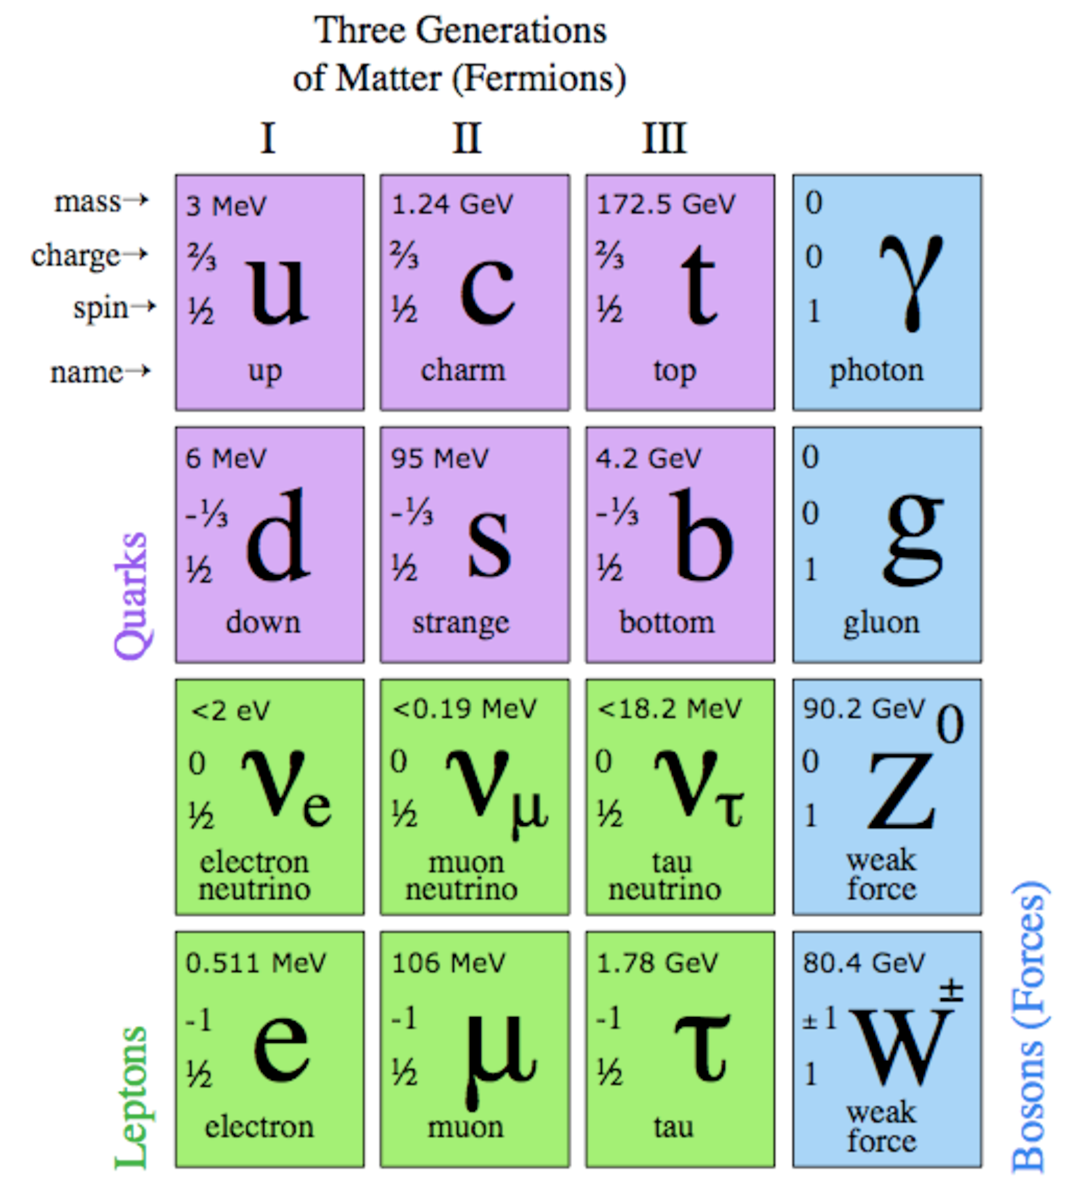
\includegraphics[scale=0.5]{SM_particlesComplete.pdf}
\caption[Summary of Standard Model particles and forces.]{The building blocks of the Standard Model: six types of quarks, six types of leptons, and four force-mediating bosons. Each quark and lepton has an antiparticle with identical mass but opposite electric charge. The final piece of the puzzle, the Higgs particle, has yet to be seen.
\label{fig_SMparticlesComplete}}
\end{figure}

The quarks are arranged in three generations. The 2\textsuperscript{nd} and 3\textsuperscript{rd} generations are heavier copies of the 1\textsuperscript{st} generation. The same is true with the leptons.

\vspace{-0.015\textheight}
\begin{singlespace}
\begin{itemize}
\item {1\textsuperscript{st} generation --- The up quark ($u$) and down quark ($d$) form the first generation. Almost all visible and stable matter is composed of these two light quarks. Their antiparticles are the $\bar{u}$ ($u$-bar) and $\bar{d}$ ($d$-bar).}
\item {2\textsuperscript{nd} generation --- The charmed quark ($c$) and strange ($s$) quark and their antiparticles, $\bar{c}$ and $\bar{s}$, form the 2\textsuperscript{nd} generation.}
\item {3\textsuperscript{rd} generation --- The top ($t$) and bottom ($b$) quarks and their antiparticles, $\bar{t}$ and $\bar{b}$, form the 3\textsuperscript{rd} generation. The top quark is the heaviest of all quarks with a mass of 173.3~$\pm$~1.1~\massunits according to the latest measurements~\cite{pap:TopMass}.}
\end{itemize}
 \end{singlespace}

The six types of quarks are called \newterm{flavors}. Each flavor of quark has one of three values of \newterm{color} charge. The color charge can be red, blue, and green for particles, and antired, antiblue, and antigreen for antiparticles.

There are six leptons: three charged and three neutral (see Fig.~\ref{fig_SMparticlesComplete}). The leptons are assumed to be point-like particles and so far there is no evidence of any internal structure. The muon ($\mu^{-}$) and tau ($\tau^{-}$) are heavier replicas of the lightest lepton, the electron ($e^{-}$). Electrons are the most abundant of the three and are found in ordinary matter. There are three corresponding neutrinos ($\nu$): the electron neutrino ($\nu_{e}$), muon neutrino ($\nu_{\mu}$), and tau neutrino ($\nu_{\tau}$). Neutrinos are assumed to be massless point-like particles in the SM. However, recent experimental evidence suggests they may have tiny mass \cite{pap:PDG}. The SM assumes quarks and leptons to be spin-1/2 particles. Particles with half-integer spin are termed \newterm{fermions}, which follow Fermi--Dirac statistics. Fermions obey the Pauli Exclusion Principle, which states that no two identical fermions may occupy the same quantum state simultaneously. Particles with integer spin are termed \newterm{bosons} and follow Bose--Einstein statistics. Bosons, unlike fermions, are not required to obey the Pauli Exclusion Principle. As mentioned earlier, hadrons are formed by combining quarks and antiquarks. In forming such combinations, one has to conserve quantum numbers such as baryon number, lepton number, color charge, and electric charge.

%%%%%%%%%%%%%%%%%%%%%%%%%
Interactions among fundamental particles can be classified in many ways. Historically this was done on the basis of their strengths. This leads to four types of interactions: \newterm{strong}, \newterm{electromagnetic}, \newterm{weak}, and \newterm{gravitational}.

The Standard Model has proposed four force-mediating particles. The photon ($\gamma$), a massless particle with no electric charge, mediates electromagnetic interactions as described by Quantum Electrodynamics (QED). The \newterm{gluon} is a massless particle that engages in strong interactions between color-carrying particles. Lastly, the \W and \Z bosons are believed to facilitate the weak interactions.  These are massive particles that can change the flavor of quarks and thereby the quark composition of particles.  Figure~\ref{fig:SMinteractions} illustrates these interactions. Finally, the gravitational force is assumed to be mediated by the \newterm{graviton}, but the SM does not account for gravity in its formulation, as it is very weak. The details of these interactions will be discussed in the next chapter. Table~\ref{tab:summary_of_four_forces} summarizes these forces and their behavior.

\begin{figure}[htb!]
\centering
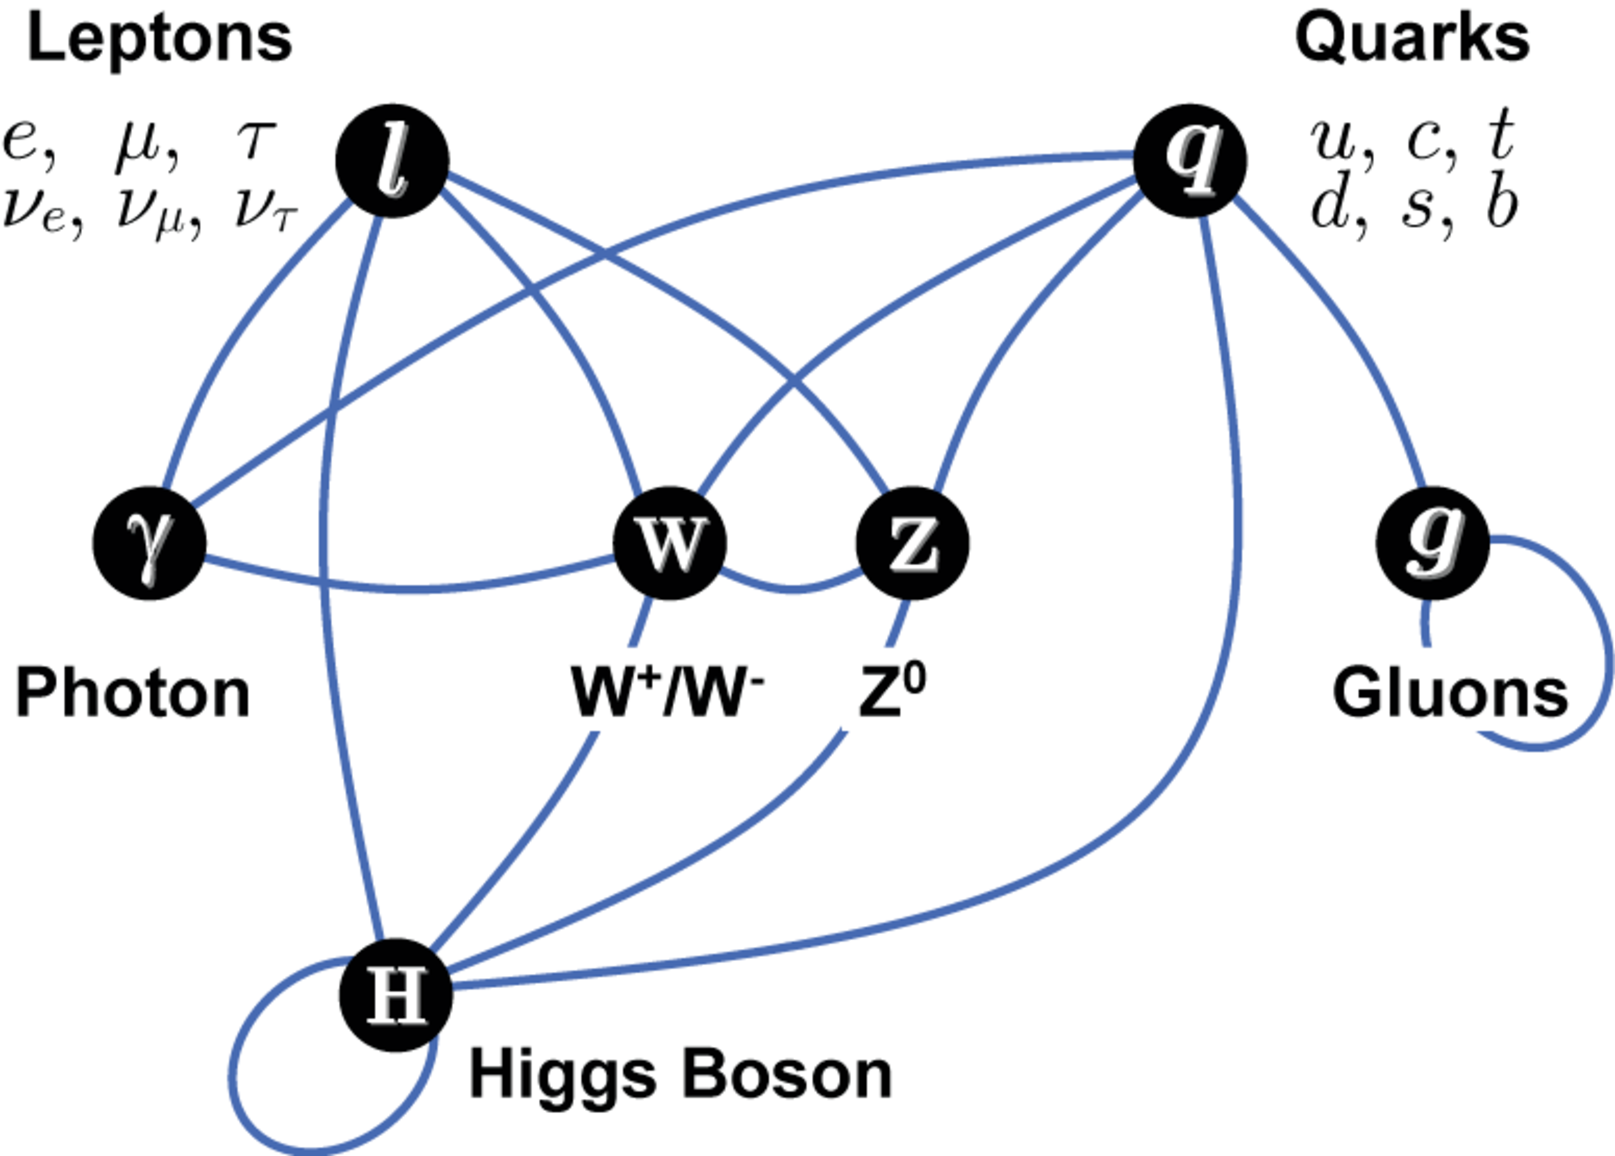
\includegraphics[scale=0.35]{Interactions.pdf}
\caption[Standard Model particles and force interactions.]{Diagram illustrating the possible interactions between elementary particles in the Standard Model. Vertices (darkened circles) represent types of particles, and the blue arcs connecting them represent possible interactions. The top row of vertices (leptons and quarks) are the matter particles; the second row of vertices (photon, $W$, $Z$, and gluon) are the force-mediating particles; the bottom row is the Higgs boson \cite{img_Interactions}.
\label{fig:SMinteractions}}
\end{figure}

\begin{table}[fhbt!]
\caption{Summary of the four fundamental forces with their relative strengths and range. The relative strength is given with respect to the strength of the graviton. This table should only be used to understand the concepts involved, as the exact numbers are under constant scrutiny.}
\label{tab:summary_of_four_forces}
\centering
\begin{tabular}{lccccc}
\hline
\BUbf{Interaction} & \BUbf{Strong} & \BUbf{Electromagnetic} & \BUbf{Weak} & \BUbf{Gravitation}\\
\hline
\multirow{2}{*}{\BUbf{Theory}} & \multirow{2}{*}{QCD} & \multirow{2}{*}{QED} & Electroweak & General \\
& & & Theory & Relativity \\[1ex]
\BUbf{Mediators} & gluon ($g$) & photon ($\gamma$) & \W and \Z bosons & graviton \\[1ex]
\BUbf{Relative} & \multirow{2}{*}{$10^{38}$} & \multirow{2}{*}{$10^{36}$} & \multirow{2}{*}{$10^{25}$} & \multirow{2}{*}{1} \\
\BUbf{Strength} & & & &\\[1ex]
\BUbf{Long Distance} & \multirow{2}{*}{1} & \multirow{2}{*}{$\frac{1}{r^2}$} & \multirow{2}{*}{$\frac{1}{r} e^{-m_{W,Z} r}$} & \multirow{2}{*}{$\frac{1}{r^{2}}$} \\
\BUbf{Behavior} & & & & \\[1ex]
\BUbf{Range} & $10^{-15}$ & $\infty$ & $10^{-18}$ & $\infty$ \\
\hline
\end{tabular}
\end{table}

The electromagnetic and gravitational interactions have been known for a long time, as they are a part of our daily life in the macroscopic world. This is because they are long range interactions (compared to the size of the nucleus, which is $\sim$10$^{-12}$~cm). This long range behavior was explained by the introduction of the concept of a field, which is assumed to have an independent existence and most importantly, contains energy. It was James Maxwell in 1864 who took this idea and explained light as a propagating electromagnetic field. With the development of quantum mechanics, the field concept became more profound and explicit. In quantum mechanics, particles may have a dual particle-like and wave-like behavior as explained by Schr\"{o}dinger in 1926. Furthermore, this wave-like behavior implied that a particle's behavior cannot be predicted definitely; one can only determine probabilities of possible outcomes.

A charged object is assumed to constantly emit and absorb photons. For example, an electron passing by a proton might intercept such a photon, absorbing its momentum and thus changing course. The existence of these photons about a charged particle is possible due to Heisenberg's uncertainty principle, which says that position and momenta cannot be simultaneously measured to arbitrarily high precision. This led to the energy-time uncertainty $\Delta E \Delta t\gtrsim h$, where $h=4.1\times10^{-15}$~eV$\cdot$s is the Planck constant, which allows particles to exist for extremely short times without being required to abide by the law of conservation of energy. They are known as \newterm{virtual particles}. Essentially, virtual particles are an artifact of quantum field theory (QFT), in which the interactions between real particles are formulated by the exchange of virtual particles.

The Standard Model has no clear answers to some of the questions like why there are two extra families of leptons and quarks or why there are only three families altogether, why gravity is so weak, and why there is no prediction of the masses of quarks and leptons. Hence, a further understanding of these fundamental particles and their interactions is needed. But this is no easy task, as these particles do not exist in normal circumstances. In order to study them, they need to be produced artificially. In 1905, Einstein pointed out the mass-energy equivalence, $E=mc^{2}$, where $E$ is the energy, $m$ is the mass, and $c$ is the speed of light in a vacuum. This relationship implies that in order to create a particle at rest with a mass $m$, one needs an equivalent amount of energy given by $E=mc^{2}$. This brought the era of collider experiments. In collider experiments, two beams of particles are collided at high energies to produce these fundamental particles for closer observation. These collisions are studied using state-of-the-art detectors like the Collider Detector at Fermilab (CDF).

In order to answer some of the questions mentioned so far, an emerging technique known as a signature-based search is used to find new physics beyond what is predicted by the SM. This thesis is arranged as described below.

In the next chapter, the SM is further discussed to provide an overview of the present understanding of particle physics. It also explains the shortcomings of the SM. Then, a competing theory that extends the \SMtext, \GMSBtext (GSMB), is explained. This chapter also describe the underlying concepts of signature-based searches. Furthermore, it explains the photon + jets signature in both the SM and GSMB.

In Chapter 3, the experimental apparatus, the CDF detector, is explained in detail. The ``Monte Carlo Event Simulation'' chapter (Chapter 4) describes how a hard collision between two hadrons is understood and how such collisions are simulated. Chapter 5, titled ``Object Reconstruction and Identification,'' explains how final-state particles or ``objects'' such as electrons, positrons, photons, and jets are reconstructed in the detector. It also describes how additional physics quantities like missing transverse energy are derived from the reconstructed particles. In the ``Datasets and Event Selection'' chapter (Chapter 6), the data used in this analysis, including when and how they were collected, are described. Furthermore, it explains the selection criteria of photon + jets events for this analysis. The ``Background Modeling'' chapter (Chapter 7) explains processes in which a photon and jets are produced. The processes that produce real photons and fake photons in association with jets are elaborated upon. It also explains two methods of background modeling. The following chapter (Chapter~8) lists and explains possible systematic uncertainties and how they are quantified.

In the ``Results'' chapter (Chapter 9), the findings of this analysis and the implications of the results are discussed in detail. All measured physics quantities are shown with associated systematic uncertainties. In the last chapter (Chapter~10), the conclusion of this search for new physics is presented.
\label{chp:Intro}

%%%%%%%%%%%%%%%%%%%%%%%%%%%%%%%%
\chapter{Theory}\label{chp:Theory}
%\glossary{name=Standard Model, description=Standard Model}
\vspace{0.015\textheight}
In this chapter, the benchmark theory of elementary particle physics, the Standard Model (SM), is further described with the focus on different interactions. Then, some limitations of the SM are described. A prominent theory model, Supersymmetry (SUSY), which attempts to supersede the SM, is introduced as a motivation for this study. Next, the philosophy of signature-based searches and their advantages are described, and this leads to a motivation for the study of the photon + jets signature. Finally, photon + jets production under the SM and SUSY is explained.

\section{Fundamental Interactions}
\vspace{0.03\textheight}
\subsection{Electromagnetic Interaction}
It should be evident now that the electromagnetic (EM) interaction occurs via the exchange of photons. Particles with charge, positive or negative, may interact with other charged particles by exchanging photons. Particles with the same charge tend to repel each other, whereas particles with opposite charge tend to attract. The photon is massless and travels at the speed of light. Quantum Electrodynamics (QED), an abelian gauge theory with the symmetry group U(1), successfully describes all phenomena involving charged particle interactions via the exchange of photons. The electromagnetic \newterm{coupling}, or the strength of the interaction, is given by $\alpha_{em} = \frac{e^{2}}{4\pi\epsilon_{0}\hbar c} = \frac{1}{137}$, where $e$ is the electric charge of the electron, $\epsilon_{0}$ is the permitivity of free space, $\hbar$ is the reduced Planck constant, and $c$ is the speed of light. Figure~\ref{fig:LeptonInteraction} shows the interaction of an electron with a photon, where the photon is absorbed or emitted and the electron's momentum is changed. QED is one of the few complete and most accurate theories to date.

\begin{figure}[htb!]
 \centering
 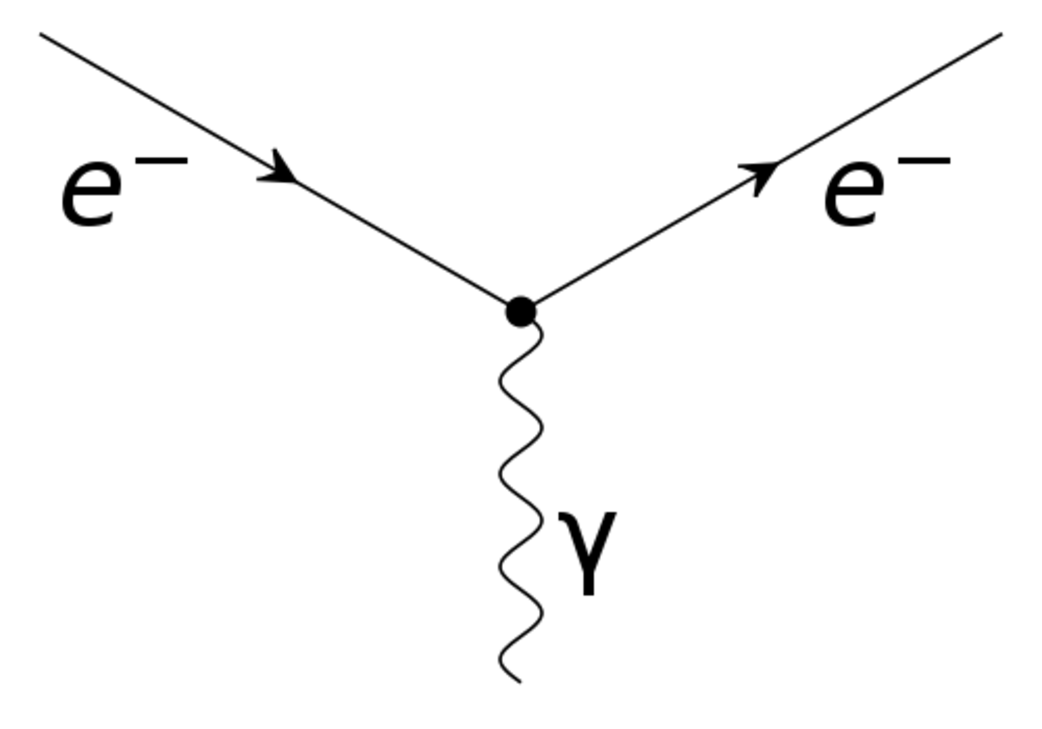
\includegraphics[scale=.25,keepaspectratio=true]{./LeptonInteraction.pdf}
 % LeptonInteraction.png: 500x350 pixel, 72dpi, 17.64x12.35 cm, bb=0 0 500 350
 \caption{Electron-photon interaction.}
 \label{fig:LeptonInteraction}
\end{figure}

\subsection{Strong Interaction}\label{sec:StrongInteraction}
As mentioned in the previous chapter, a fundamental question of the early explorers of the nucleus was how nuclei can stay stable with so many positively charged protons packed within a distance of a few femtometers (1 fm = $10^{-15}$ m). The answer was a force much stronger than the electromagnetic interaction, but with a very short range confined to the nuclear scale. This force is called the \newterm{strong} force. The strong force carriers, gluons, mediate the interactions between the quarks. The color charge of quarks, in addition to their electric charge, allow them to participate in strong interactions. Both gluons and quarks carry the color charge. Gluons are the quanta of the color field that bind quarks in nucleons and also nucleons into nuclei. Strong interactions preserve the color charge and are mathematically explained by the non-abelian SU(3) gauge symmetry under Quantum Chromodynamics (QCD). At the strong interaction scale of $\Lambda \sim$~200~MeV, the hadrons are composed of quarks and gluons. The \newterm{strong coupling}, which defines the strength of the strong interaction, is energy scale dependent, i.e. at higher energies the coupling decreases as in Eq.~\ref{eqa:QCDasymptoticFreedom}. This is termed \newterm{asymptotic freedom} (see Fig.~\ref{fig:RunStrongCoupling}).

\begin{figure}[p]
 \centering
 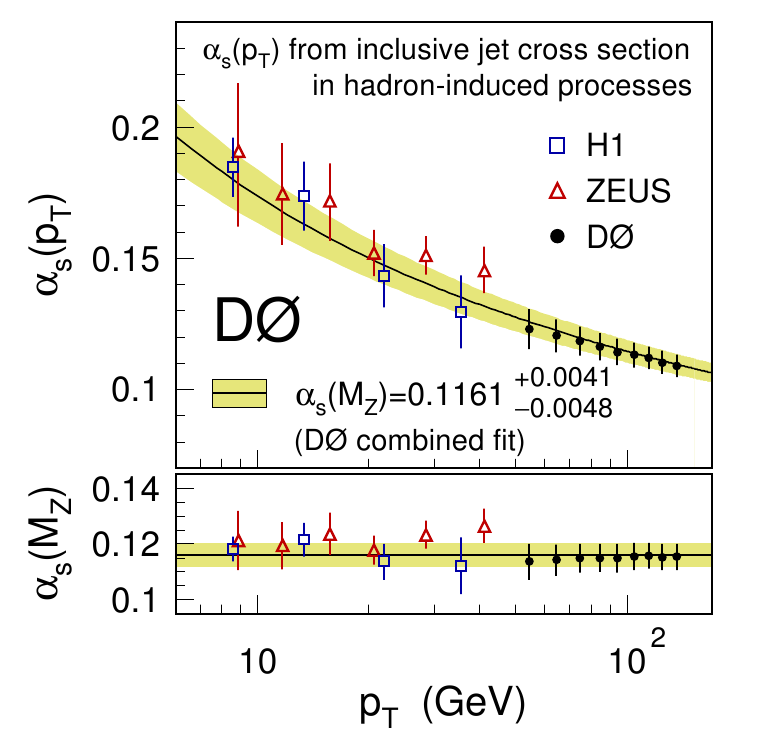
\includegraphics[scale=0.75]{./RunningStrongCoupling.png}
 % RunningStrongCoupling.png: 770x739 pixel, 96dpi, 20.37x19.55 cm, bb=0 0 577 554
 \caption{A recent D\O~measurement of the strong coupling constant, $\alpha_{s}$, as a function of \pt (top) and at the mass of the $Z$ boson, $M_Z$ (bottom). Measurements from the HERA experiment are overlaid for comparison. The error bars indicate combined statistical + systematic uncertainties~\cite{pap:D0_StrongCoupling}.}
 \label{fig:RunStrongCoupling}
\end{figure}

Asymptotic freedom allows the study of QCD processes using perturbation theory at high energies (see Section~\ref{sec:pQCD}). The coupling parameter of QCD interactions (\alphas) is a \newterm{running} constant (energy dependent) and to lowest order is described by Eq.~\ref{eqa:QCDasymptoticFreedom}. Here, $N_{f}$ is the number of quark flavors, $\Lambda$ is the QCD scale parameter, and $Q^{2}$ is the momentum transfer (energy) scale.

\begin{equation}
 \alpha_{s} (Q^{2}) =\frac{12\pi}{(33 - 2 N_{f})\log(Q^{2}/\Lambda^{2})}
 \label{eqa:QCDasymptoticFreedom}
\end{equation}

Quarks are not observed individually, but are always bound with other quarks or antiquarks in composite particles. If one attempts to separate quarks that are close to each other, they form color-neutral particles: mesons or baryons. This property of quarks and antiquarks to combine to form color-neutral particles is known as \newterm{color confinement}.

\begin{figure}[htb!]
 \centering
\subfigure[]{
 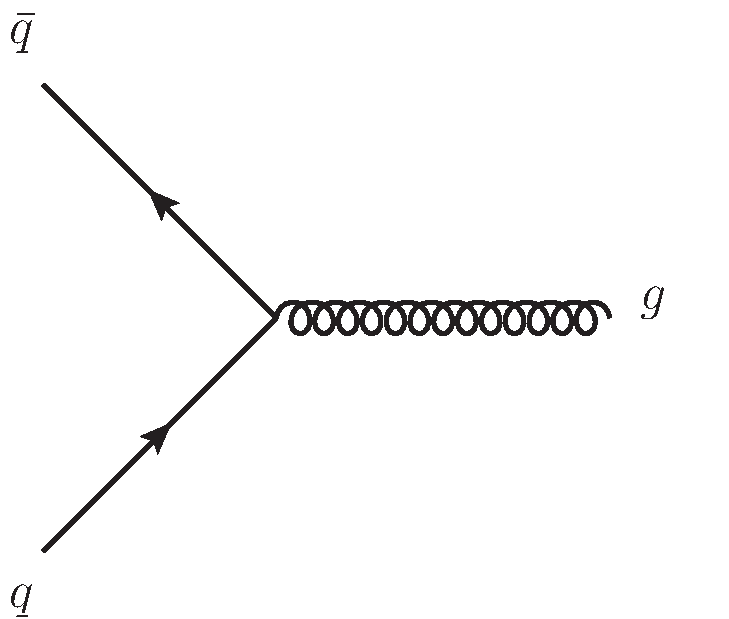
\includegraphics[scale=0.3,keepaspectratio=true]{images/QCD_vertices_1.pdf}
}
\subfigure[]{
 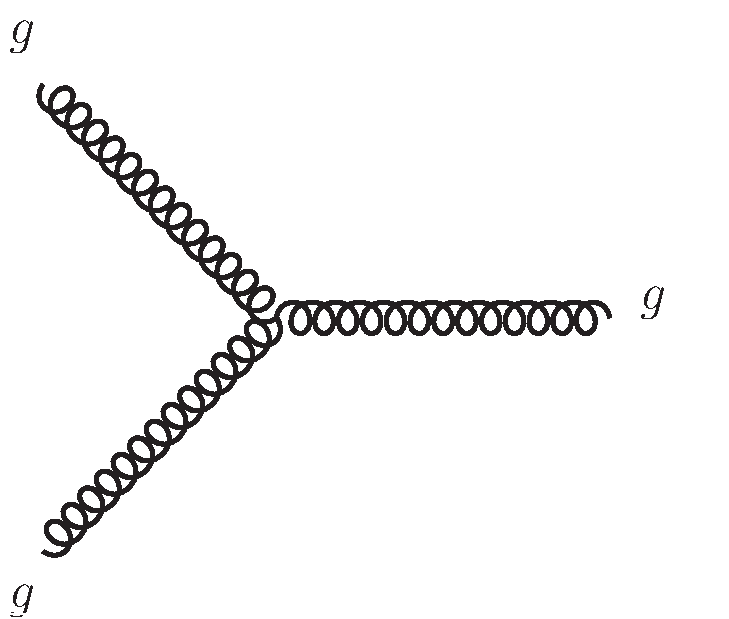
\includegraphics[scale=0.3,keepaspectratio=true]{images/QCD_vertices_2.pdf}
}
\subfigure[]{
 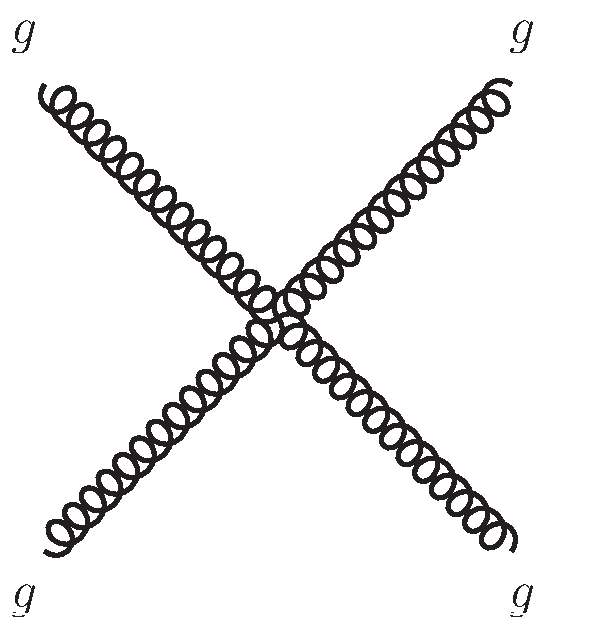
\includegraphics[scale=0.3,keepaspectratio=true]{images/QCD_vertices_3.pdf}
}
\caption{Quark and gluon interaction vertices under QCD.}
\label{fig:FeynQCDGluonCoupling}
\end{figure}

As shown in Fig.~\ref{fig:FeynQCDGluonCoupling}, the gluons (\particle{g}) can couple only to quarks or other gluons. The QCD Lagrangian is defined by
\begin{equation}
 {\cal L}_{QCD} = -\frac{1}{4} F_{a}^{\mu\nu} F_{a\mu\nu}+\bar{\Psi_{j}}(i\gamma_{\mu}D^{\mu}_{jk}-M_{j}\delta_{jk})\Psi_{k}
%X_i^{\phantom{i}j}\\\%this is a much better tech to get the superscript and subscript gets the same size
%X^j_{\phantom{j}i}\\
\end{equation}
where $D^{\mu}_{jk}$ is the covariant derivative given by
\begin{equation}
 D^{\mu}_{jk} = \delta_{jk}\partial^{\mu}+ig(T_{a})_{jk}G_{a}^{\mu}
\end{equation}
and $F_{a}^{\mu\nu}$ is the gluon field tensor, $\Psi_{k}$ represents the quark fields, $M$ represents the quark mass matrices, $g$ is the strong coupling constant, $G_{a}^{\mu}$ represents the gluon fields, and the $T$ are SU(3) generators. They follow the commutation relationship
\begin{equation}
 [T_{i},T_{j}]=if_{ijk}T_{k}.
\end{equation}
Here, the $f_{ijk}$ are the QCD structure constants. The \newterm{gamma matrices} ($\gamma$) are defined in the Dirac representation as:

\begin{equation*}
 \gamma^{0}=\left(
\begin{array}{ccc}
I & 0\\
0 & -I
\end{array}
\right),\quad
\gamma^{i}=\left(
\begin{array}{ccc}
0 & \sigma_{i}\\
-\sigma_{i} & 0
\end{array}
\right),\quad
\gamma^{5}=\left(
\begin{array}{ccc}
0 & I\\
I & 0
\end{array}
\right),
\end{equation*}
where $I$ is the $2\times2$ identity matrix and $\sigma_{i}$ are the Pauli matrices,
\begin{equation*}
 \sigma_{1}=\left(
\begin{array}{ccc}
0 & 1\\
1 & 0
\end{array}
\right),\quad
\sigma_{2}=\left(
\begin{array}{ccc}
0 & -i\\
i & 0
\end{array}
\right),\quad
\sigma_{3}=\left(
\begin{array}{ccc}
1 & 0\\
0 & -1
\end{array}
\right).
\end{equation*}

\subsection{Electroweak Interaction}
The electromagnetic and strong forces were enough to understand and explain many aspects of nature. However, the proposal of the \newterm{weak force} by Enrico Fermi solved the mystery of \newterm{beta decay},\footnote{Spontaneous emission of an electron or a positron by a nucleon in the atomic nucleus} which baffled scientists for a long time. The weak force allows a quark to change its flavor by exchanging a virtual boson (a $W$ or a \Z boson). The weak interactions of the first generation of leptons are shown in Fig.~\ref{fig:WeakInteractionVertices}. One of the major achievements of the SM is that the electromagnetic and the weak interaction are described by a single theory, the electroweak theory. The discovery of the \W and \Z intermediate vector bosons at CERN gave tremendous support to the theory. The \newterm{electroweak interaction} is implemented by a gauge theory based on the SU(2)$_\mathrm{L}$~$\times$ U(1)$_\mathrm{Y}$ group (where the \textit{L} indicates that the weak force couples only to the \newterm{left-handed} particles). A particle is \newterm{right-handed} if the direction of its spin is the same as the direction of its motion (see Fig.~\ref{fig:Helicity}). It is left-handed if the directions of spin and motion are opposite. %This group symmetry is spontaneously broken via the Higgs mechanism.

\begin{figure}[h]
 \centering
\subfigure[]{
 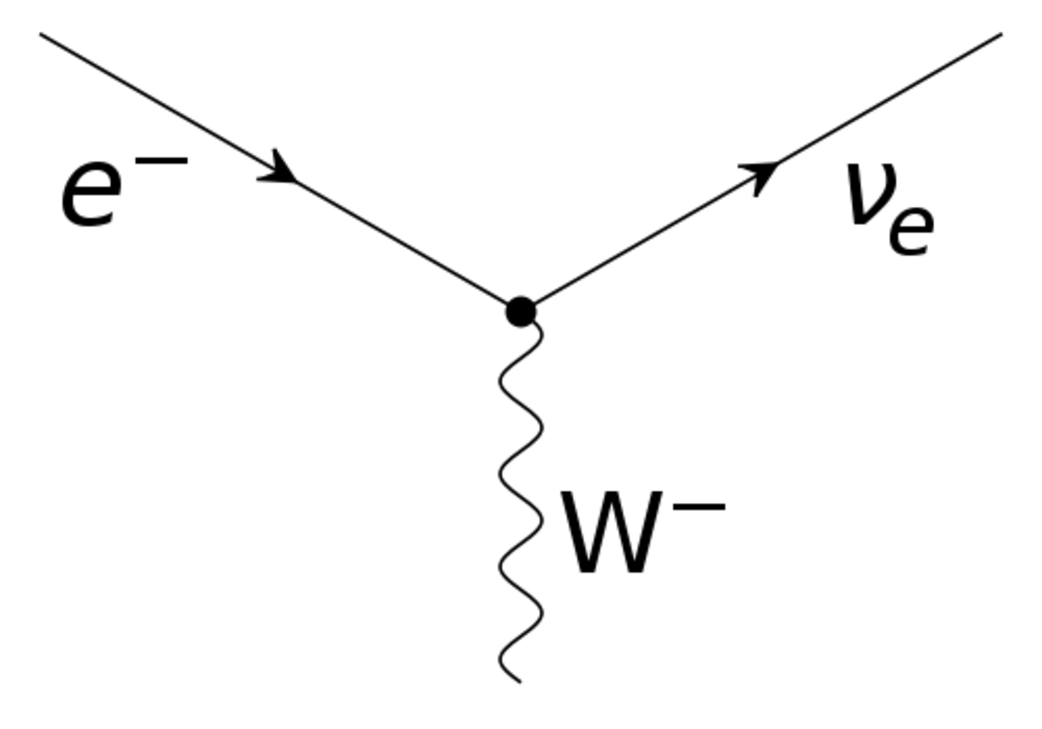
\includegraphics[scale=0.25,keepaspectratio=true]{./WeakInteractionVertex1.pdf}
}
\subfigure[]{
 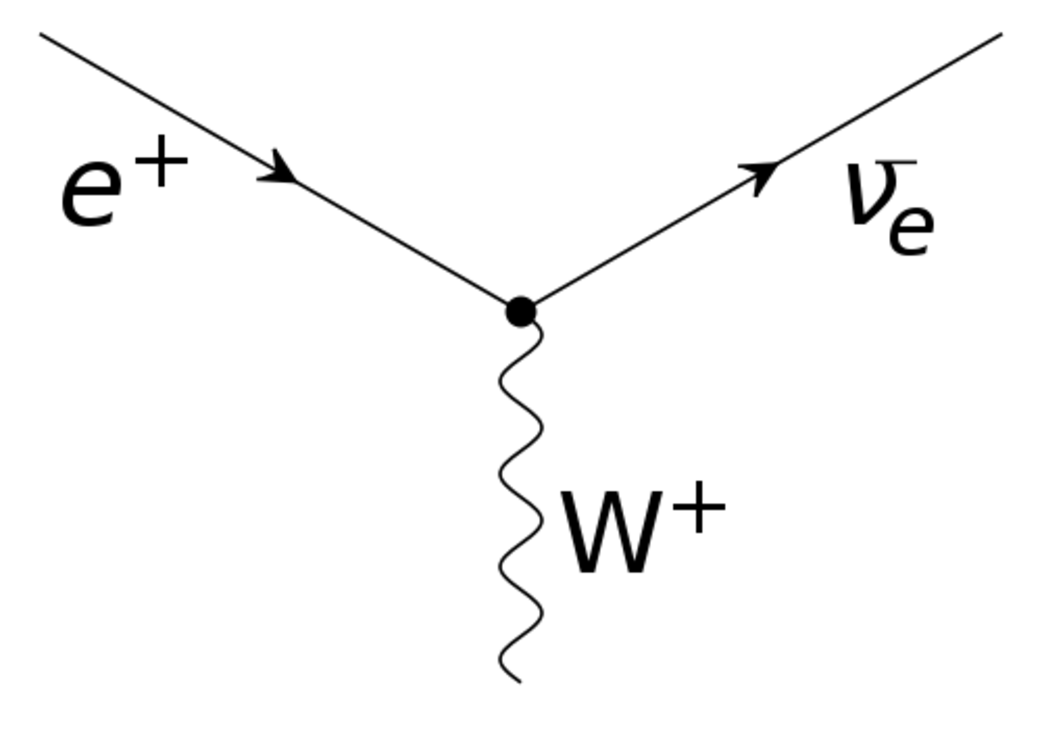
\includegraphics[scale=0.25,keepaspectratio=true]{./WeakInteractionVertex2.pdf}
}
\subfigure[]{
 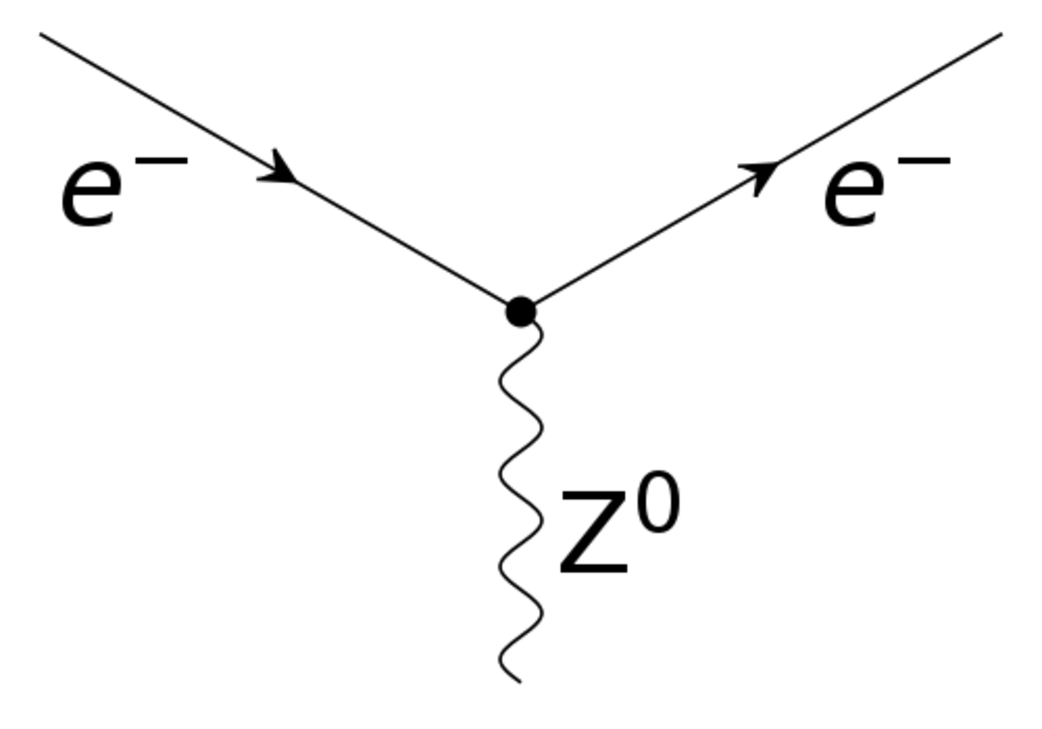
\includegraphics[scale=0.25,keepaspectratio=true]{./WeakInteractionVertex3.pdf}
}
 \caption{Weak interaction vertices of the first generation leptons.}
 \label{fig:WeakInteractionVertices}
\end{figure}

\begin{figure}[h!]
\vspace{3ex}
 \centering
 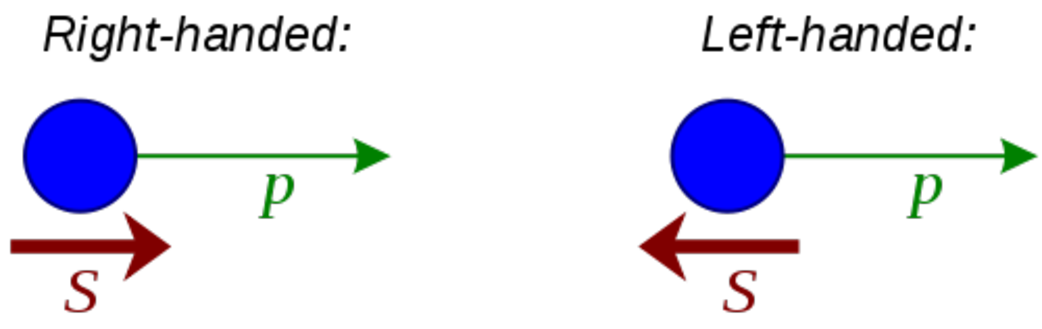
\includegraphics[scale=0.8,keepaspectratio=true]{./Helicity.pdf}
 % Helicity.png: 500x158 pixel, 72dpi, 17.64x5.57 cm, bb=0 0 500 158
 \caption{A particle is left-handed or right-handed based on the alignment of its spin ($S$) and momentum ($p$).}
 \label{fig:Helicity}
\end{figure}

The \newterm{weak interaction} is due to the exchange of the heavy \W and \Z bosons. For example, beta decay is possible only via the weak interaction. In reality, a down quark in a neutron ($udd$) decays into an up quark, converting it to a proton ($uud$) via an exchange of $W^{-}$ boson. The $W^{-}$ boson subsequently decays into a electron ($e^{-}$) and an electron antineutrino ($\bar\nu_{e}$). The weak interaction allows a quark to change its flavor by emission or absorption of a vector boson (\W). A lepton or a quark can readily absorb or emit a \Z boson without changing its flavor.

\subsection{Gravity}
Gravity is described here only for the completeness of the discussion. Gravity is by far the weakest of all the forces (see Table~\ref{tab:summary_of_four_forces}). As a result, it has no measurable effect on a subatomic scale. So far, the SM has not been able to extend its Lagrangian to incorporate gravity. In addition, the force-mediating particle of gravity, the graviton, has yet to be discovered.

\subsection{Unification of Forces}
Similar to the unification of the electromagnetic and weak interactions into the electroweak theory, \newterm{Grand Unification Theories} (GUTs)~\cite{pap:GUTtheory} predict that the SM fundamental interactions (electromagnetic, weak, and strong) unite at an extremely high energy scale (see Fig.~\ref{fig:TOE_ForceUnified}). Unifying gravity with the other three interactions forms a \newterm{Theory of Everything} (TOE) \cite{pap:TOE}.

\begin{figure}[p]
 \centering
 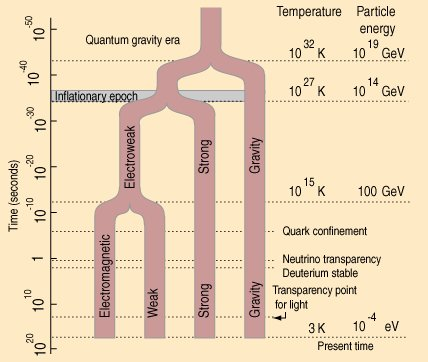
\includegraphics[scale=0.99 ,keepaspectratio=true]{./guts_forceUnification2.jpg}
 % guts_forceUnification.png: 540x476 pixel, 72dpi, 19.05x16.79 cm, bb=0 0 540 476
 \caption[Unification of the fundamental forces at extremely high energies.]{A theoretical prediction of the unification of the fundamental forces at extremely high energies. The energy limit of current particle accelerators is about 10$^{12}$~eV, making it impossible to test such theories.}
 \label{fig:TOE_ForceUnified}
\end{figure}

\subsection{Higgs Mechanism}\label{sec:EWKSymmetryBreaking}
The SM proposes that the mass of the observed particles arises from the interaction (coupling) of particles with the \newterm{Higgs field}, which has a non-zero \newterm{vacuum expectation value} (VEV). A naive picture is that the Higgs field exerts some amount of resistance as the particles traverse the field, and hence the field gives rise to the inertial mass that is observed. The resistance is different for different particles. Of course, other kinds of interactions like the strong interaction can contribute to the resulting measured mass.

The Higgs mechanism was incorporated into the SM to generate masses for the heavy vector bosons and eventually the lighter fermions. This was achieved by breaking the electroweak symmetry via Higgs mechanism. As a result a new scalar particle (spin-0) called the Higgs boson is predicted.

The Higgs boson (\particle{H}) is the only particle predicted by the SM that has yet to be observed experimentally. Like all other particles, the Higgs boson acquires its mass by interacting with the Higgs field. Direct searches at the Tevatron and LEP (Large Electron-Positron Collider at CERN) have shown the mass of the \particle{H} to be greater than 114~\massunits. Recent Tevatron data have excluded a Higgs mass between 158~$<M_{H}<175$~\massunits at the 95\% confidence level \cite{pap:HiggsLimits}.

\section{Limitations of the \SMtext}
The SM has been tested extensively by experimental data. So far, no evidence contradicting SM predictions has been observed. Yet, there are many questions that are not addressed or verified by the SM. If one compares the strength of the four fundamental forces (see Table~\ref{tab:summary_of_four_forces}), it is evident there are two widely separated scales. The gravitational force is proportional to the inverse of the distance squared, yet its interaction is associated with a huge mass scale called the \newterm{Planck scale} ($\sim$10$^{19}$~GeV), which makes the interactions very weak. On the other hand, the \newterm{electroweak scale} (\mbox{$\sim$246 GeV}) sets the masses for $W$ and $Z$ bosons to be $\sim$80~\massunits and $\sim$91~\massunits, respectively. This, in its simplest manifestation, is known as the \newterm{hierarchy problem}.

\begin{figure}[htb!]
 \centering
\subfigure[]{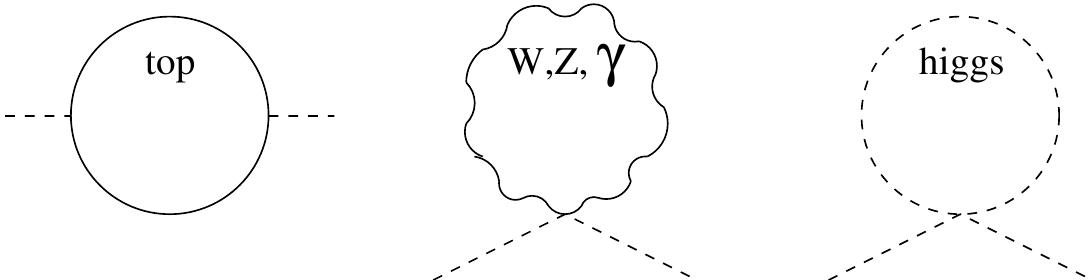
\includegraphics[keepaspectratio=true,scale=0.5]{./SMHiggsDivergentContributions.png}}\\[1ex]
\subfigure[]{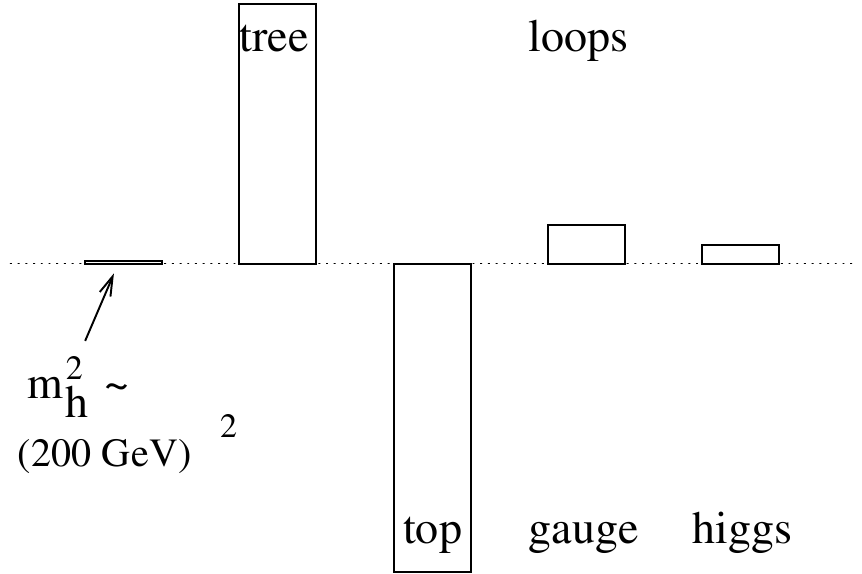
\includegraphics[keepaspectratio=true,scale=0.4]{./CorrectionsToHiggsMass2.png}}
\caption{(a) The most significant quadratically divergent contributions to the Higgs mass in the Standard Model and (b) the fine tuning required to obtain an acceptable Higgs mass in the Standard Model with cut-off 10~TeV.}
\label{fig:SMHiggsDivergentContributions}
\end{figure}

Another manifestation of the hierarchy problem is the undesirable large loop corrections to the Higgs mass as shown in Fig.~\ref{fig:SMHiggsDivergentContributions}. Furthermore, although there is plenty of evidence for electroweak symmetry breaking, the exact mechanism is not confirmed and the Higgs boson's existence has not been verified. In addition to these, there are other questions that need to be answered. Below are some of those questions.
\vspace{-0.01\textheight}
\begin{singlespace}
\begin{enumerate}
 \item It provides no prediction of the masses of the fundamental particles: the quarks and leptons.
 \item It does not explain the existence of two extra families of leptons and quarks, nor why there are only three families.
 \item It does not explain why gravity is so weak, and it is not able to describe its effects at the quantum level.
 \item The neutrinos were assumed to be massless. Yet recent experimental results show evidence of neutrino oscillations, which indicate that neutrinos may have a tiny but non-zero mass.
 \item There is no natural candidate for \newterm{dark matter}. Cosmology and astronomy suggests that 70\% of the universe is \newterm{dark energy} and another 25\% is made of \newterm{dark matter}, meaning only 5\% of visible matter is explained by the SM.
\end{enumerate}
\end{singlespace}

There are numerous new theory models attempting to address these shortcomings, like \newterm{Supersymmetry} (SUSY) and \newterm{Technicolor} \cite{pap:TechnicolorModel}. Since the production of a photon in association with jets is so fundamental, it is present in almost all such theory models. Among those theory models, SUSY has become a leading candidate and is being extensively studied by physicists.

\section{Supersymmetry (SUSY)}\index{SUSY}
Supersymmetry is one of the promising theory models attempting to supersede the SM. It is described in detail in the literature \cite{pap:SUSY_SMartin, pap:SUSY_IJRAitchison}. It assumes there is another physical symmetry beyond those included in the SM. By the introduction of heavier partners for all SM particles, SUSY is able to cancel the unphysical large loop corrections to the Higgs mass. It also provides an answer for why the weak force is far stronger than gravity (the hierarchy problem) (see Table~\ref{tab:summary_of_four_forces}). Furthermore, by unifying three of the SM gauge interactions (the weak interaction, strong interaction, and electromagnetic interaction) and having natural candidates for the dark matter, it is appealing to study.

\subsection{SUSY Particles}
The theory proposes the existence of supersymmetric particles (superpartners) for all the \SM particles. For each type of \SM boson, there is a fermionic superpartner and vice versa as shown in Fig.~\ref{fig:SM_SUSY_Particles}. The bosonic counterparts to the SM fermions get an ``s'' prefix (lepton~$\to$``slepton'', ``quark''~$\to$ ``squark'') and the fermionic counterparts to SM gauge bosons get an ``ino'' suffix (``gauge boson'' $\to$ ``gaugino'').

\begin{figure}[htbm]
 \centering
 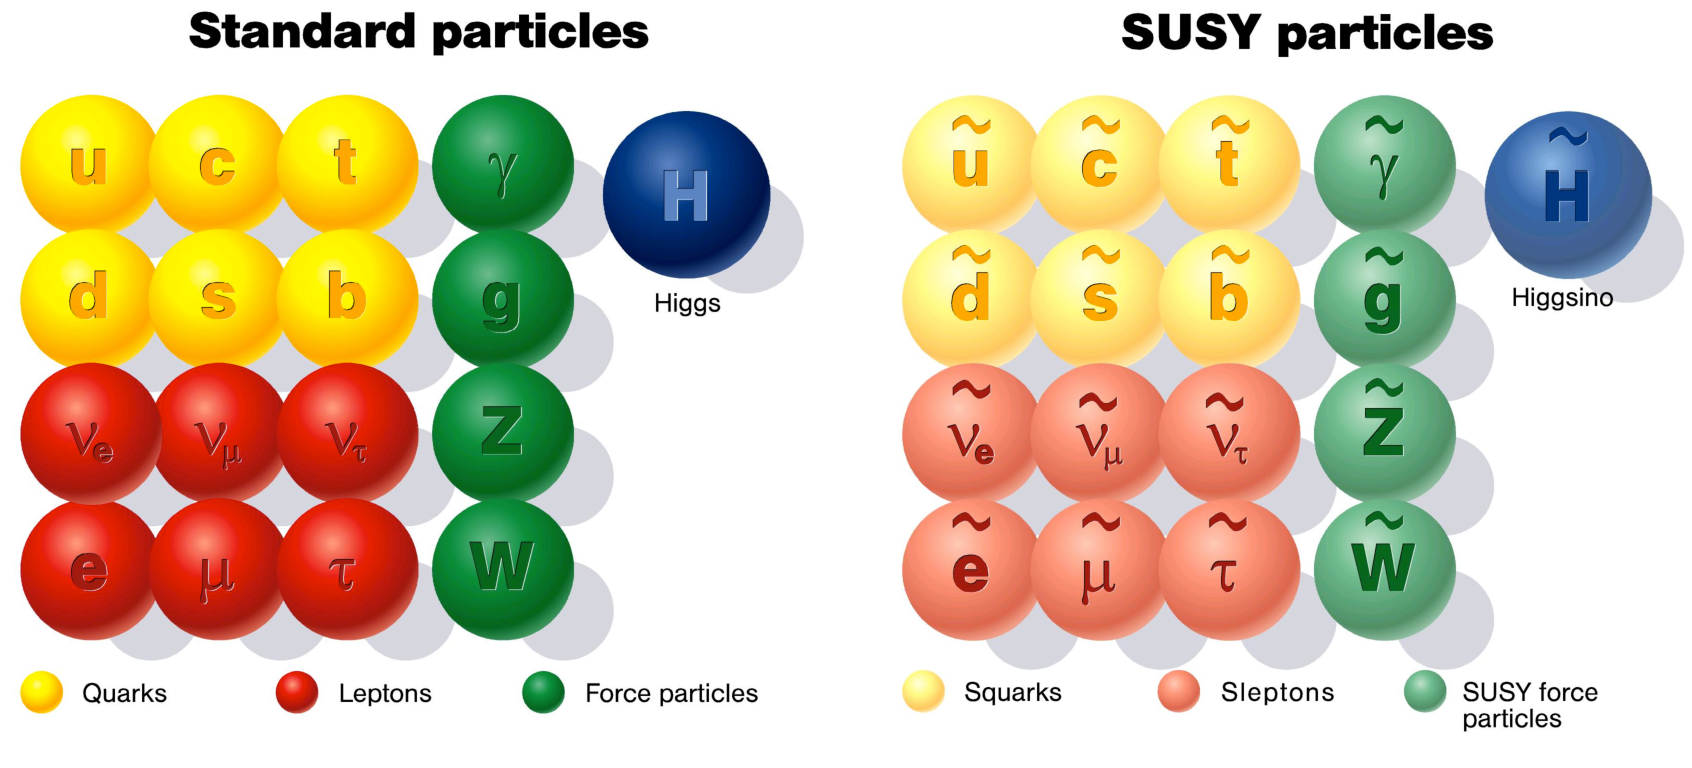
\includegraphics[keepaspectratio=true, scale=0.5]{./SM_SUSY_particles.pdf}
 % SM_SUSY_particles.jpg: 3478x1596 pixel, 300dpi, 29.45x13.51 cm, bb=0 0 835 383
 \caption[Supersymmetry particles.]{Supersymmetry partners (right) of the Standard Model particles (left).}
 \label{fig:SM_SUSY_Particles}
\end{figure}
\vspace{-0.01\textheight}

In the minimal supersymmetric extension of the \SM (MSSM) there can only be one such supermultiplet, but it has 105 unknown parameters (mass, angle, and phase parameters). The MSSM Lagrangian includes all possible supersymmetric interaction terms that satisfy SU(3)~$\times$ SU(2)~$\times$ U(1) gauge invariance and $B-L$ conservation, where $B$ is the baryon number and $L$ is the lepton number. The electric charge is defined by $Q=T_{3}+\frac{1}{2}Y$ where $T_{3}$ is the third component of the weak isospin and $Y$ is the hypercharge. The gauge supermultiplets consist of the gluons and their gluino fermionic superpartners and the gauge bosons and their gaugino fermionic superpartners. The extended Higgs sector of the MSSM is needed to guarantee cancellation of anomalies and to generate the desired quark masses. The corresponding field content of the MSSM and gauge quantum numbers are shown in Table~\ref{tab:SUSY_MSSM_Fields}.

\begin{table}
\caption{The particles (fields) in the MSSM and their quantum numbers. Only one generation of quarks and leptons are shown. For each lepton, quark, and Higgs supermultiplet, there is a corresponding antiparticle multiplet of charge-conjugated fermions and their associated scalar partners \cite{pap:PDG}.}
\label{tab:SUSY_MSSM_Fields}
\centering
\begin{tabular}{cccccc}
\hline
%\multicolumn{6}{c}{Field Content of the MSSM}\\
%\hline
\BUbf{Super-} & \BUbf{Boson} & \BUbf{Fermionic} & & & \\
\BUbf{Multiplets} & \BUbf{Fields} & \BUbf{Partners} & \BUbf{SU(3)} & \BUbf{SU(2)} & \BUbf{U(1)}\\
\hline
gluon/gluino & $g$ & $\widetilde{g}$ & 8 & 1 & 0\\[1ex]
gauge boson/ & $W^{\pm}$, $W^{0}$ & $\widetilde{W}^{\pm}$, $\widetilde{W}^{0}$ & 1 & 3 & 0\\
gaugino & $B$ & $\widetilde{B}$ & 1 & 1 & 0\\[1ex]
slepton/ & $(\widetilde{\nu},\widetilde{e}^{-})_{L}$ & $(\nu,e^{-})_{L}$ & 1 & 2 & --1\\
lepton & $\widetilde{e}^{-}_{R}$ & $e^{-}_{R}$ & 1 & 1 & --2\\[1ex]
squark/ & $(\widetilde{u}_{L},\widetilde{d}_{L})$ & $(u,d)_{L}$ & 3 & 2 & 1/3\\
quark & $\widetilde{u}_{R}$ & $u_{R}$ & 3 & 1 & 4/3\\
& $\widetilde{d}_{R}$ & $d_{R}$ & 3 & 1 & --2/3\\[1ex]
Higgs/ & $(H_{d}^{0}, H_{d}^{-})$ & $(\widetilde{H}_{d}^{0}, \widetilde{H}_{d}^{-})$ & 1 & 2 & --1\\
higgsino & $(H_{u}^{+}, H_{u}^{0})$ & $(\widetilde{H}_{u}^{+}, \widetilde{H}_{u}^{0})$ & 1 & 2 & 1\\[1ex]
\hline
\end{tabular}
\end{table}

\subsection{$R$-Parity}
Every SUSY particle is assigned a new quantum number called \newterm{R-parity}:
\begin{equation}
 R = (-1)^{3(B-L)+2S}
 \label{eqa:SUSY_Rparity}
\end{equation}
where $B$ ($L$) is its baryon (lepton) number and $S$ is the spin. The SM and the SUSY particles differ by this quantum number and all SM particles have $R=1$ while SUSY particles have $R=-1$. There are many extensions to SUSY based on conservation of or violation of $R$-parity. It is generally believed that $R$-parity is conserved as otherwise it can lead to an unacceptable fast proton decay. As a consequence, SUSY particles are produced in pairs, and a SUSY particle decays into SM particles accompanied by the lightest SUSY particle (LSP), which is proposed to be stable. Furthermore, cosmological constraints require that the LSP be neutral and colorless.

\subsection{Charginos and Neutralinos}
The mixing of the charged gauginos ($\widetilde{W}^{\pm}$) and the charged higgsinos ($H_{u}^{+}$ and $H_{d}^{-}$) is described by a complex $2\times2$ mass matrix (at tree-level) \cite{pap:SUSYCharginoMasses1, pap:SUSYCharginoMasses2}. This gives rise to non-negative chargino masses denoted by $\widetilde{\chi}^{\pm}_{1}$ and $\widetilde{\chi}^{\pm}_{2}$. These are linear combinations of the charged gaugino and higgsino states.

The mixing of the neutral gauginos ($\widetilde{B}$ and $\widetilde{W}^{0}$) and neutral higgsinos $\widetilde{H}_{u}^{0}$ and $\widetilde{H}_{d}^{0}$ is described by a complex symmetric $4\times4$ mass matrix (at tree level) \cite{pap:SUSYCharginoMasses1, pap:SUSYGauginoMasses1, pap:SUSYGauginoMasses2}. This gives rise to four physical neutralino states denoted by $\widetilde\chi_{i}^{0}$ ($i=1,..., 4$), where the states are ordered by increasing mass, $M_{\widetilde\chi_{1}^{0}} \leq M_{\widetilde\chi_{2}^{0}} \leq M_{\widetilde\chi_{3}^{0}} \leq M_{\widetilde\chi_{4}^{0}}$. The $\widetilde\chi_{i}^{0}$ are the linear combinations of the neutral gaugino and higgsino states.

\subsection{Breaking of SUSY}
There are many theory models that attempt to explain how the supersymmetry is broken so the expected masses and the interactions of the superpartners are acceptable. One of the leading candidates is the \newterm{Gauge Mediated Supersymmetry Breaking} (GMSB) method \cite{ pap:SUSY_SMartin, pap:SUSY_MDine1993}. In GMSB, SUSY is broken at very high energies, in a \newterm{hidden sector} that introduces SUSY-breaking interactions to the \newterm{visible} gauginos and scalars. Then, all SUSY counterparts are either heavier than their SM counterparts or are too weakly interacting.
In GMSB, the LSP is fixed to be the gravitino ($\widetilde{G}$). The $\widetilde{G}$ mass is typically in the eV range. The $\widetilde{G}$ is also considered as a potential dark matter candidate in the recent literature \cite{pap:DarkMatterCandidates}.

So far there has been no experimental evidence of superpartners. This could possibly be due to the inaccessibility of high masses with current particle accelerators. The Large Hadron Collider (LHC) at CERN has the potential of such discoveries as it reaches the design center of mass energy of 14~TeV over the next few years.

%%%%%%%%%%%%%%%%%%%%%%%%%%%%%%%%%%%%%%%%%%%%%%%%
% IDEA OF SIGNATURE BASED SEARCH
%%%%%%%%%%%%%%%%%%%%%%%%%%%%%%%%%%%%%%%%%%%%%%%%
\section{The Signature-Based Search}
Given the large number of theoretical models proposed with many free parameters, it is virtually impossible to test all of them explicitly. A \textit{signature-based} search is one way to search for new physics beyond the present theoretical understanding, which is currently described by the Standard Model. A signature is defined by the final-state particles --- those particles that we can measure in the detector. In a signature-based search, a certain decay process and decay products are studied by measuring the final-state particles. Starting with a certain level of understanding of the kinematics of the process, one examines kinematic distributions of the final-state particles for an anomalous behavior of observed data.

The selection of a signature has strong theoretical motivations. Incompleteness of the SM provides a tremendous motivation for a search like this. The selection of a signature is based on several factors. One deciding factor is the amount of data available with the required final-state particles. This will directly affect the precision of the final measurements and also the sensitivity. The detector's ability to identify and reconstruct particular particles will contribute. Another motivation for studying a particular signature might be inconclusive results of a previous study. For example, the recent inclusive photon + jet + $X$ (anything) cross section measurement has shown differences between data and theory \cite{pap:PhoJetCrosssection_D0}. Authors were unable to explain the dependence of the cross section on $p_{T}^{\gamma}$ over the whole measurement range.

There are many advantages to doing a signature-based search. Instead of optimizing the data analysis for a particular theoretical model and searching only a narrow region of phase space, one instead searches the entire phase space accessible via the data. By doing so, a global sensitivity to any anomaly, not just an anomaly associated with a particular theoretical model, can be achieved. Because the final measurement presents the behavior of the data as it is, the measurement never becomes obsolete and future models can even be tested using the data (provided there is complete information such as the efficiency and acceptance for measured objects). An added bonus of a signature-based search is that it can easily spawn new searches. A search can be easily expanded by requiring additional final-state objects. For example, a search for photon + jets can be extended to photon + electron + jet or photon + \particle{b}-quark jet.

There are some downsides to a signature-based search. Not optimizing for any particular model could mean less sensitivity to observing evidence for it. There is no measure of efficiency or the acceptance for objects associated with a decay mode. Hence, the final results may be less precise and less valuable to theorists.

\section{Photon + Jets Signature}
This thesis studies the physics of \ppbar collisions that produce a photon and jets as final-state particles. Section \ref{sec:gjetProdInSM} describes the production of a photon in the SM, which can lead to a photon + jets signature in the detector. During the initial parton interaction, a photon is radiated by the incoming or outgoing quark (antiquark). A photon produced directly from the incoming or outgoing quark (antiquark) is known as a \newterm{prompt photon}. The outgoing partons (quarks or gluons) will be observed as jets in the detector. Furthermore, it is possible for the incoming or outgoing partons to radiate extra gluons or photons, and those will be measured as additional jets and photons in the detector. However, such emissions are suppressed by the coupling strengths.

In the leading-order $2\to2$ SM process, the photon and jet are produced back-to-back in the center of mass frame of the incoming partons, as seen in Fig. \ref{fig:gjet_topology}. Because the incoming partons only have momentum along the $z$ axis, the momenta of the photon and jet must be balanced in the transverse plane.\footnote{The transverse plane is chosen for convenience of measurements. This eliminates the difficulty of measuring the longitudinal momentum of the incoming partons.} The presence of extra jets or photons will change this back-to-back topology. Also, it should be noted that SM $\gamma$ + jet processes show no undetectable particles that can produce an energy imbalance in the transverse plane.

\begin{figure}[htbm]
 \centering
\subfigure[]{\label{fig:gjet_toplogy_cm}
 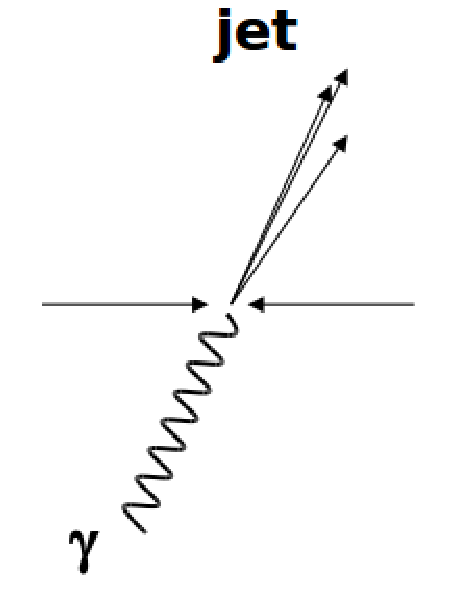
\includegraphics[scale=.6,keepaspectratio=true]{images/backtoback_gjet_cm_demo.pdf}
}
\subfigure[]{\label{fig:gjet_toplogy_lab}
 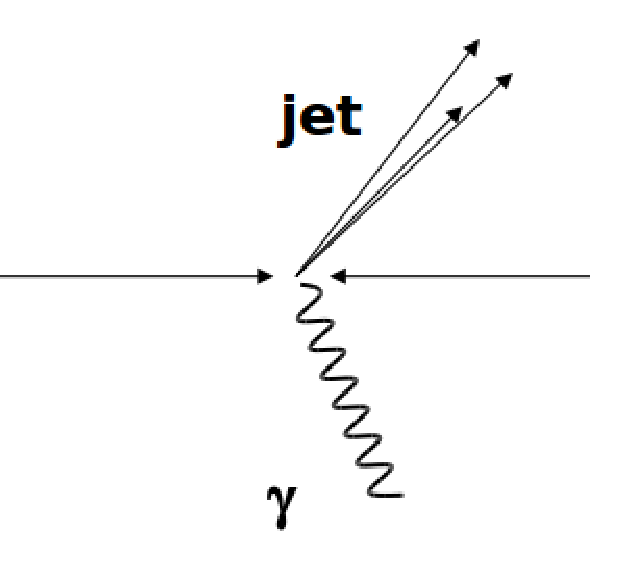
\includegraphics[scale=.6,keepaspectratio=true]{images/backtoback_gjet_lab_demo.pdf}
}
\caption{Topology of a $\gamma$ + jet event. (a) The $\gamma$ and jet are produced back-to-back in the center of mass frame of the incoming partons. (b) The $\gamma$ and jet are boosted (along the $z$ axis into lab frame).}
 \label{fig:gjet_topology}
\end{figure}
\vspace{-0.02\textheight}

The study of prompt photons has several advantages. Prompt photons emerge directly from the hard scattering process without undergoing fragmentation. Hence, by studying these photons, it is possible to extract parent parton information. Since the photon is a well understood elementary particle that interacts via the electromagnetic force, its energy can be measured with high accuracy to avoid a large systematic uncertainty associated with jet identification. Furthermore, photons are easier to identify using the detector's trigger system, and photon reconstruction is relatively simple.

By studying data events with a photon and jets, the presence of a new decay process or a new heavy particle may become evident by a sudden increase in the number of observed events in a narrow region of a distribution or distributions. A weakly interacting particle, like the hypothesized $\widetilde{G}$ in the decay of $\widetilde{\chi}^{0}_{1}\to\gamma \widetilde{G}$ in GMSB, is likely to produce an excess of data events with a large energy imbalance in the transverse plane.

\subsection{Photon + Jets Production in the SM}\label{sec:gjetProdInSM}

\begin{figure}[p]
\begin{center}
\subfigure[Annihilation]{
\label{fig:SM_pj_annihilation}
\begin{tabular}{cc}
\raisebox{0\height}{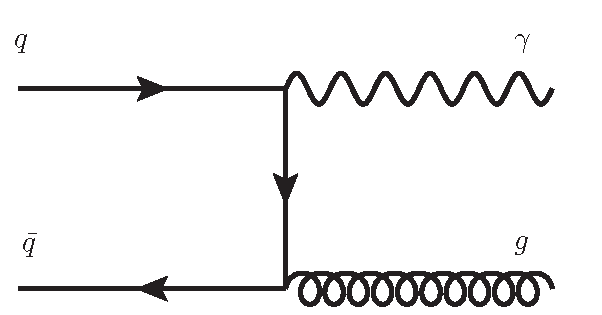
\includegraphics[scale=0.5]{images/Feyn_gjet_annihilation.pdf}} &
\raisebox{0\height}{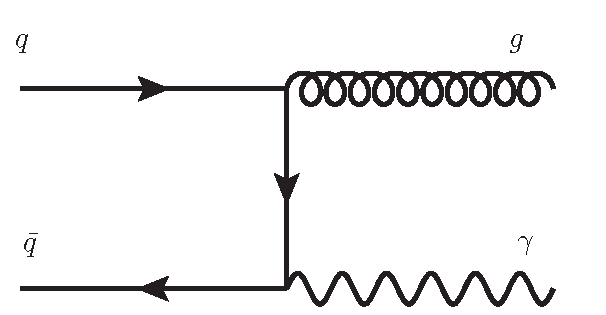
\includegraphics[scale=0.5]{images/gjets_qq2gpho_annihilation3.pdf}}\\
\multicolumn{2}{c}{\raisebox{0\height}{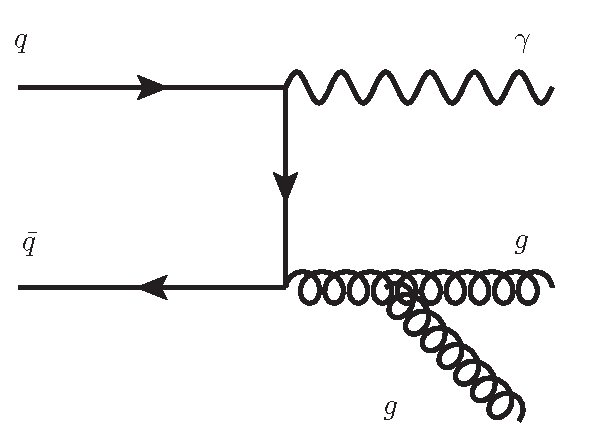
\includegraphics[scale=0.5]{images/Feyn_gjets_annihilation.pdf}}}
\end{tabular}
}
\subfigure[Compton Scattering]{
\label{fig:SM_pj_compton}
\begin{tabular}{cc}
\raisebox{0.1\height}{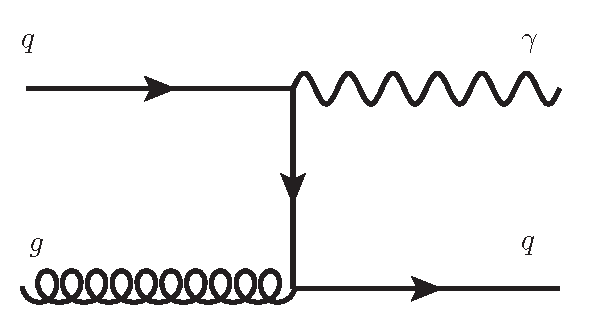
\includegraphics[scale=0.5]{images/Feyn_gjet_compton.pdf}} &
\raisebox{0.0\height}{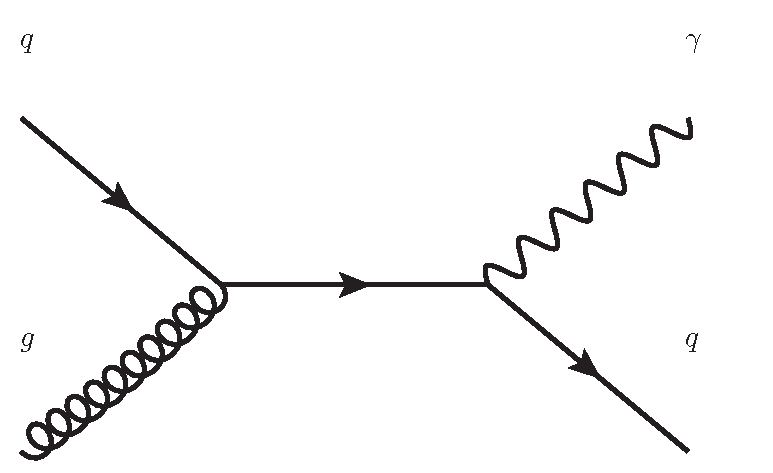
\includegraphics[scale=0.4]{images/gjets_qg2phoq_compton2.pdf}}\\
\raisebox{0.0\height}{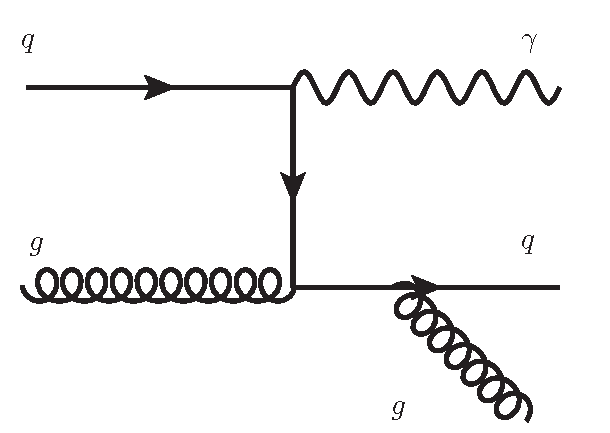
\includegraphics[scale=0.5]{images/Feyn_gjets_compton.pdf}}&
\raisebox{0.0\height}{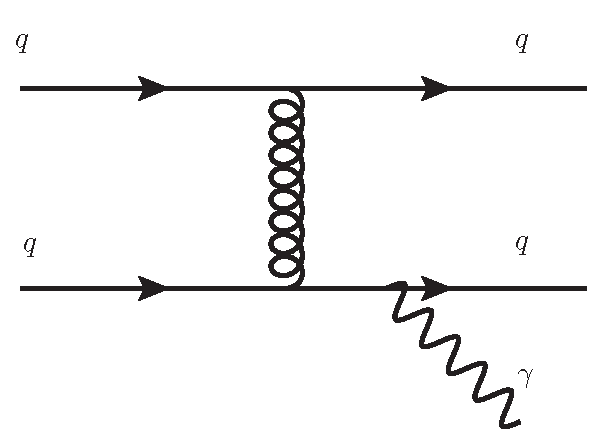
\includegraphics[scale=0.5]{images/gjets_qq2qq_compton.pdf}}
\end{tabular}
}
\subfigure[Bremsstrahlung Radiation]{
\label{fig:SM_pj_brem}
\begin{tabular}{cc}
\raisebox{0.3\height}{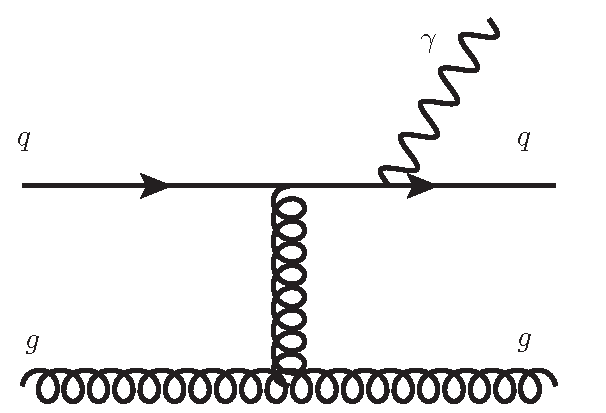
\includegraphics[scale=0.5]{images/Feyn_gjet_brem.pdf}} &
\raisebox{0.0\height}{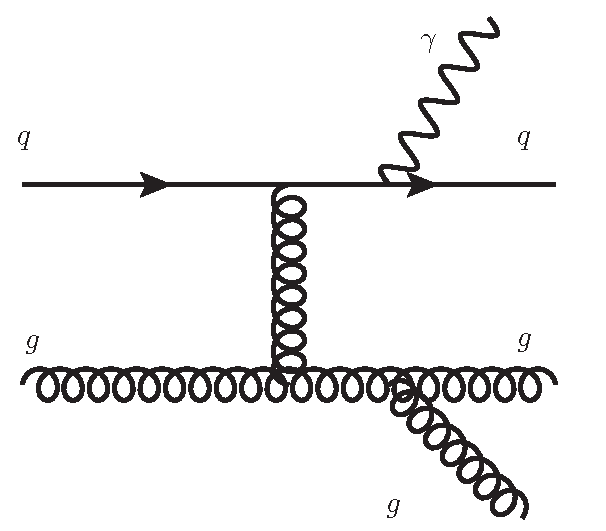
\includegraphics[scale=0.5,keepaspectratio=true]{images/Feyn_gjets_brem.pdf}}
\end{tabular}
}
\end{center}
\caption{Leading-order and next-to-leading-order Feynman diagrams for Standard Model prompt photon production. Next-to-leading-order production will have extra gluon radiation and/or gluon exchanges.}
\label{fig:SM_pj_Feynmans}
\end{figure}

The SM production of photons ($\gamma$) is a radiative process in which a photon is emitted either from an initial-state parton or from a final-state parton. This can happen only through a quark, which is electrically charged and can couple to a photon via the electromagnetic interaction (QED). The partons (quarks and/or gluons) will proceed to interact via the strong force. This prompt photon production can be divided into two components, a direct component (Fig.~\ref{fig:SM_pj_annihilation} and Fig.~\ref{fig:SM_pj_compton}) and bremsstrahlung (Fig.~\ref{fig:SM_pj_brem}). To lowest order, at large photon momentum, the inclusive cross section is dominated by the following two subprocesses:
\begin{eqnarray}
\mathrm{Compton:} && q(\bar{q}) + g \to \gamma + q(\bar{q})\\
\mathrm{Annihilation:} && q + \bar{q} \to \gamma + g
\label{eqa:gjets_ComptAnnihilation}
\end{eqnarray}
To lowest order, the invariant cross section for the subprocess
\begin{equation}
 a+b\to c+\gamma
\end{equation}
can be written as
\begin{equation}
 E_{\gamma}\frac{d\hat{\sigma}}{d^{3}p_{\gamma}} = \frac{\hat{s}}{\pi}\frac{d\sigma}{d\hat{t}}\delta(\hat{s}+\hat{t}+\hat{u})
\end{equation}
where $\hat{s}$, $\hat{t}$, and $\hat{u}$ are the Mandelstam variables \cite{pap:JFOwens_RevModPhy59465_1987} for the subprocess. The elementary cross sections for the leading-order processes (${\cal O}(\alpha_{s})$) are
\begin{eqnarray}
 \frac{d\sigma}{d\hat{t}} (q + g \to \gamma + q) &=& -\frac{\pi\alpha\alpha_{s}}{3{\hat s}^{2}} e^{2}_{q} \frac{{\hat u}^{2}+{\hat s}^2}{{\hat u}{\hat s}}\\
 \frac{d\sigma}{d\hat{t}}(q + \bar{q} \to \gamma + g) &=& -\frac{8\pi\alpha\alpha_{s}}{9{\hat s}^{2}} e^{2}_{q} \frac{{\hat u}^{2}+{\hat t}^2}{{\hat u}{\hat t}}
\end{eqnarray}
where $e_{q}$ is the charge of the interacting quark. Although the two components are topologically distinct, interference effects make them inseparable. Still, one can gain insight into these processes by measuring the separation between the objects and the softness of their energies.

Isolated photons from photon + jets production come largely unaltered from the hard scattering process. Hence, they can be used to directly probe the hard scattering dynamics. At low transverse momentum of the photon, the Compton scattering process $qg\to q\gamma$ dominates. This process probes the gluon density of the colliding hadrons at low momenta where gluons carry the bulk of the momentum. At higher transverse momenta, quark and antiquark annihilation $q{\bar q}\to g\gamma$ becomes the dominant process.

Final-state quarks and gluons will hadronize to form stable particles, and will be observed as a collimated spray of particles called a jet. At the detector level, these events would be reconstructed as a photon plus one or more jets. The initial-state and final-state partons can radiate additional gluons to produce more jets.

The emission of a $\gamma$ is due to a point-like QED coupling that provides a unique opportunity to study the partons more closely, specifically the gluon content of the protons and antiprotons.

It is important to note that there is no intrinsic missing energy present in these processes. Any measured missing energy would be most likely due to mismeasurements. But a significant number of events with large missing energy could also indicate new physics.

\begin{figure}[htbm]
 \centering
 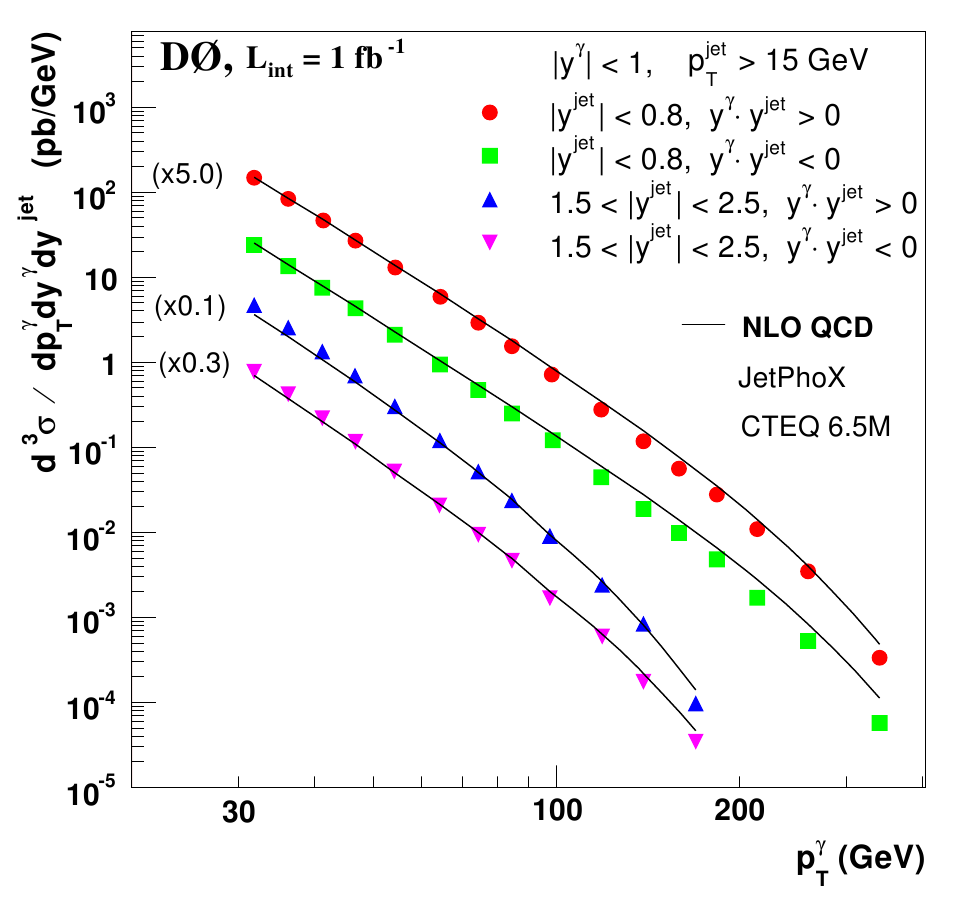
\includegraphics[scale=0.45,keepaspectratio=true]{./PhoJets_Crosssection.png}
 % PhoJets_Crosssection.png: 646x612 pixel, 96dpi, 17.09x16.19 cm, bb=0 0 484 459
 \caption{Differential cross section of $\ppbar\to\gamma+\mathrm{jet}+X$ measured as a function of the transverse energy of the photon $p_{T}^{\gamma}$. $X$ represents any other physics object(s) not identified in the event. The photon is required to have \ptg{30.0} and \etalessthan{1.0}, and the jet is required to have \ptg{15.0} and \etalessthan{2.5}. Cross sections are measured in four regions of rapidity $y$. For presentation purposes, some distributions are scaled by the factors shown along the side of each curve. The black lines correspond to the theoretical predictions
 \cite{pap:PhoJetCrosssection_D0}.}
 \label{fig:PhoJetCrosssection}
\end{figure}
\vspace{-0.02\textheight}

Figure~\ref{fig:PhoJetCrosssection} describes a recent measurement of the photon + jets cross section as a function of the transverse energy of the photon. It is worth comparing the scale of the photon + jets cross section to the cross section for jet production shown in Fig.~\ref{fig:ProductionCrosssections}. Figure~\ref{fig:ProductionCrosssections} shows the cross sections of some of the physics processes at different center of mass energies. These probabilities depend on the luminosity as demarcated on the right hand axis. This example shows the overwhelmingly large number of physics processes and the difficulty of isolating rare processes.

\begin{figure}[htmb]
 \centering
 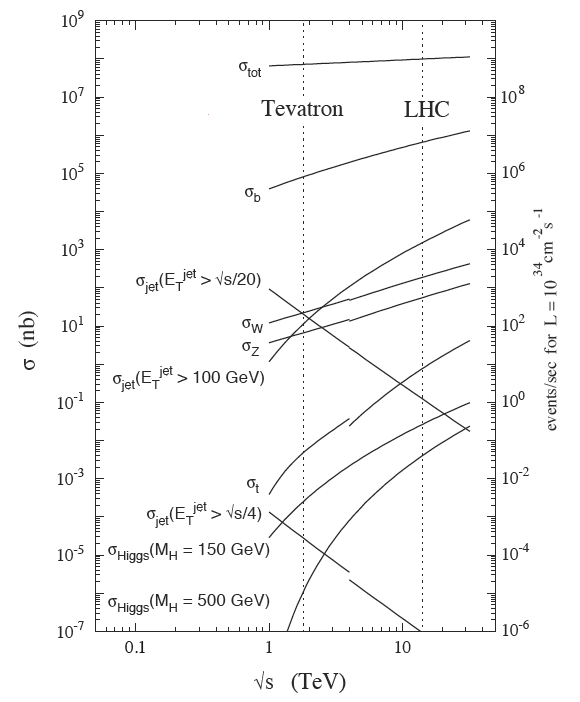
\includegraphics[scale=0.55,keepaspectratio=true]{./ParticleCrossSections.png}
 % ParticleCrossSections.pdf: 408x518 pixel, 72dpi, 14.39x18.27 cm, bb=0 0 408 518
 \caption{Cross sections for some physics processes at the Large Hadron Collider (LHC) at CERN \cite{www:LHCPublic} and the Tevatron at Fermilab \cite{www:FNALpublic}. The dotted lines show the energies of the two hadron colliders: 14~TeV at the LHC at 14~TeV and 1.96~TeV at the Tevatron \cite{www:ParticleProductionCrosssections}. Discontinuities seen for certain processes are due to the difference in colliding beams. At the LHC proton-proton beams are collided, whereas at the Tevatron proton-antiproton beams are collided. Processes dominated by gluon interactions are not changed, but the processes dominated by quarks do change, as seen by the discontinuities.}
 \label{fig:ProductionCrosssections}
\end{figure}


\subsection{Photon + Jets Production in \GMSBtext}
The Feynman diagrams shown in Fig.~\ref{fig:GMSBSUSY} show GMSB processes in which a photon and a jet(s) are produced in the final state. The SUSY particles decay into SM particles via a cascade decay. This decay will be observed as follows. A photon will be produced by $\widetilde{\chi}^{0}_{1}\to \gamma\widetilde{G}$ and the $\widetilde{G}$ will escape detection, producing a large energy imbalance. One or more of the other decay products ($\tau$) will be identified as jet(s). Using these decay products it is possible to measure the mass of the SUSY particles.

\begin{figure}[hbt!]
 \centering

\subfigure[]{
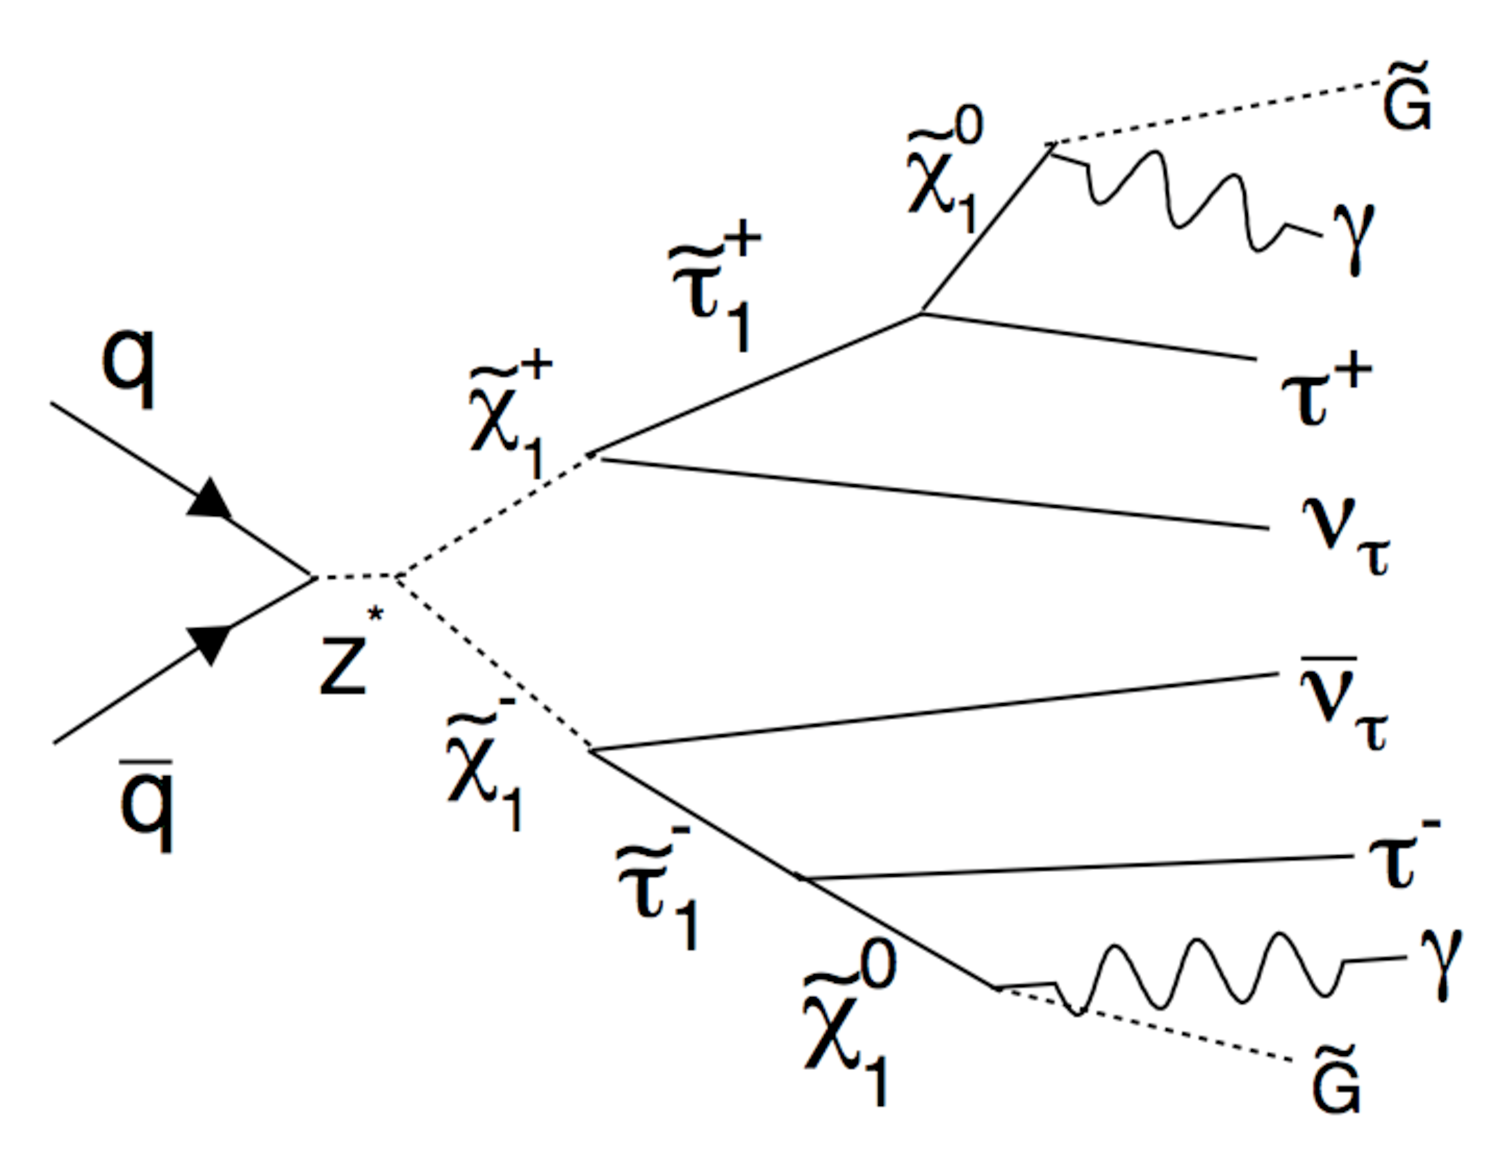
\includegraphics[scale=0.25]{images/SUSY_1.pdf}
\label{fig:SUSY_1}
}
\subfigure[]{
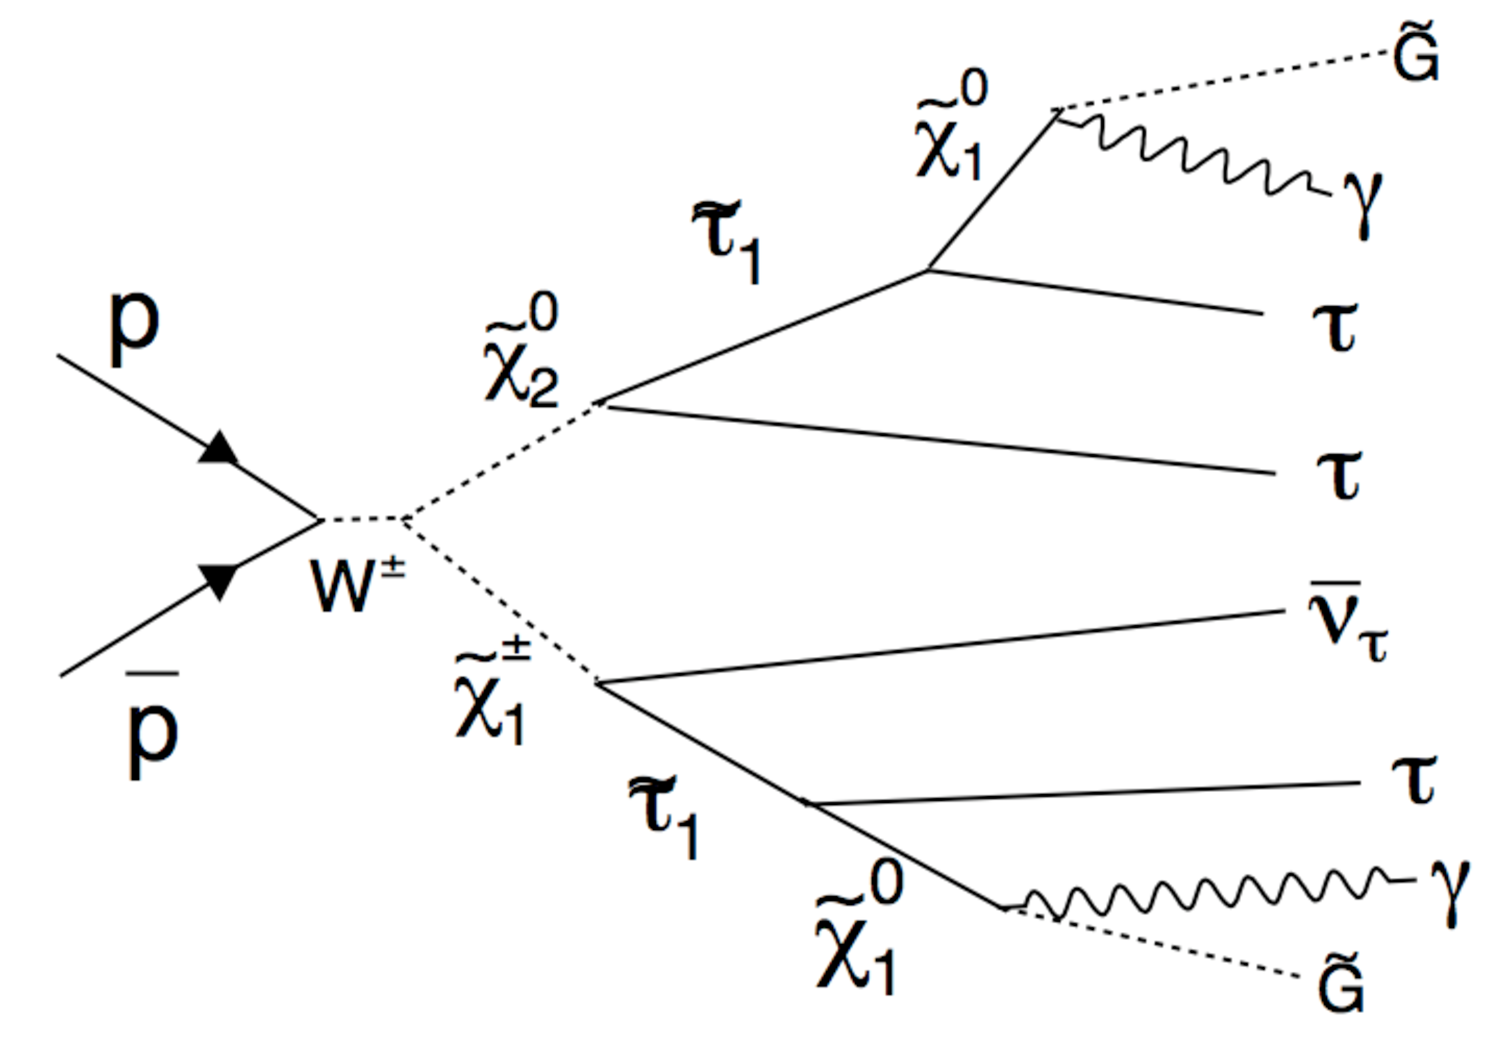
\includegraphics[scale=0.26]{images/SUSY_2.pdf}
\label{fig:SUSY_2}
}

 \caption{Predicted tree-level production mechanisms of GMSB theory.}
 \label{fig:GMSBSUSY}
\end{figure}


\chapter{The Experiment}\label{chp:Experiment}
\vspace{0.015\textheight}
This study is performed at the world's highest energy proton-antiproton collider, the Tevatron, which operates at the Fermi National Accelerator Laboratory (Fermilab) located just west of the city of Chicago. The 4-mile-long accelerator ring accelerates protons and antiprotons close to the speed of light and collides them in order to unravel mysteries of the subatomic world. An overview of the Tevatron accelerator and the Collider Detector at Fermilab (CDF) experiment, where the data are collected, is described in this chapter. Different subdetectors of the CDF detector are described together with their purpose for this analysis. In addition, some of the contributions of the author to the operation of the CDF detector subsystems is described. Finally, the method of extracting interesting physics events from hadron collisions is explained.

\section{The Tevatron}

\begin{figure}[htb!]
\begin{centering}
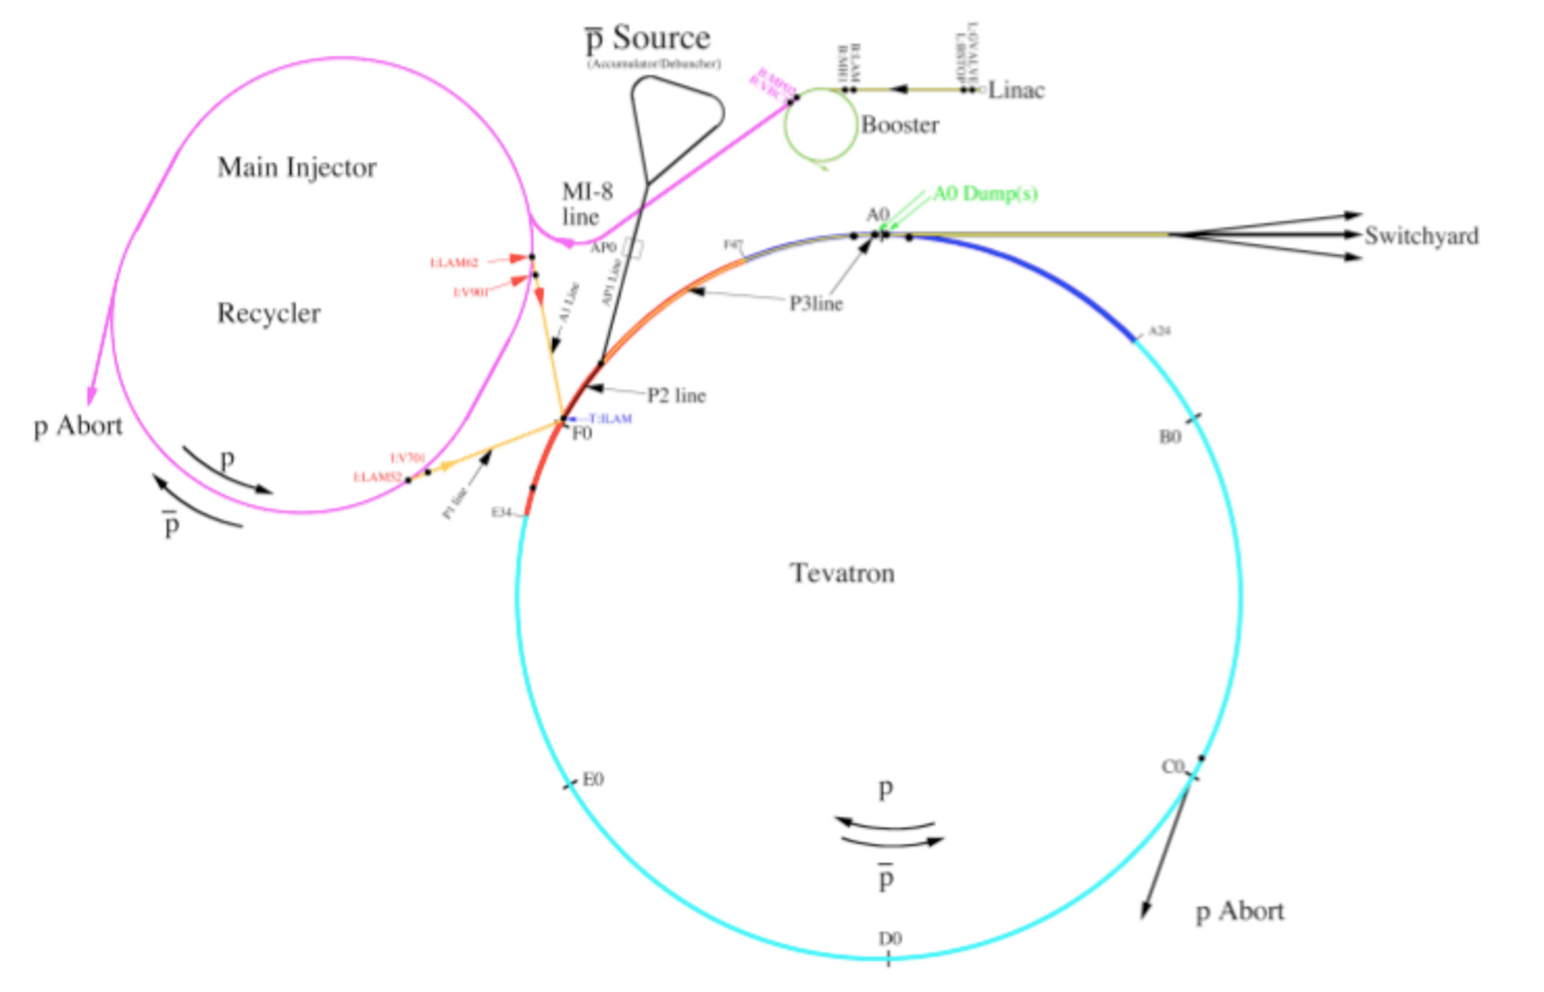
\includegraphics[scale=0.6]{AcceleratorOverview.pdf}
\caption{Overview of the accelerator complex.}
\label{fig_AcceleratorOverview}
\end{centering}
\end{figure}

The Tevatron is the largest of the Fermilab accelerators (see Fig.~\ref{fig_AcceleratorOverview}). It is a synchrotron (circular accelerator) where two particle beams, protons ($p$) and antiprotons ($\bar{p}$), circulate in opposite directions. With its eight accelerating cavities, it can accelerate protons and antiprotons up to \mbox{980 GeV}, yielding a center of mass energy ($\sqrt{s}$) of \mbox{1.96 TeV}. A large number of superconducting magnets placed along the beam pipe steer the beam around the ring. An extensive cryogenic cooling system keeps these superconducting magnets at subzero temperatures (\mbox{$\sim$4 K}). Because the magnets are superconducting, a large magnetic field can be achieved with only one-third of the power of regular magnet. The accelerated beams are collided at two points located around the the ring, at the center of the CDF and D\O~detectors.

\subsection{Pre-accelerator}
The acceleration process starts when protons are extracted from hydrogen gas in the pre-accelerator or Preacc. The Preacc houses a proton source that converts hydrogen gas to ionized hydrogen gas ($H^{-}$) that is accelerated to an energy of \mbox{750 keV} using an electrostatic potential difference. At this initial stage the Preacc accelerates the beam every \mbox{66 ms}, or at a rate of \mbox{15 Hz}. Then the beam is transfered to the next level of acceleration, the Linac.

\subsection{Linac}
The Linac is a linear accelerator that accelerates the hydrogen ions to \mbox{400 MeV} using a combination of drift tubes and radio frequency (RF) cavities. The Linac operates at the same frequency as the Preacc. Several quadrupole magnets placed inside the drift tubes, along the accelerating modules, focus the beam before handing it over to the Booster.

\subsection{Booster}
The Booster, with a \mbox{75 m} radius, is the first synchrotron in the chain of accelerators. A series of magnets are arranged around the ring, intermixed with 18 RF cavities. The Booster first strips off the electrons from the 400~MeV hydrogen ions to make protons and then it accelerates the protons to \mbox{8 GeV} of energy. The Booster operates at \mbox{15 Hz} and can accelerate the beam once every 66 milliseconds. From the Booster, the beam goes to the Main Injector.

\subsection{Main Injector}
The Main Injector (MI) is the second synchrotron in the chain with a size just over half the circumference of the Tevatron. In addition to accepting protons from the Booster, the MI also accepts antiprotons from the antiproton source. Using its 18 acceleration cavities, the MI accelerates protons from the Booster up to \mbox{150 GeV}. If it is used to accumulate antiprotons, it will accelerate them to \mbox{120 GeV}. When used to inject proton and anitprotons beams into the Tevatron, it will accelerate the beams to \mbox{150 GeV}. The MI also delivers particle beams with different energies to other experiments on site.

\subsection{Antiproton Generation}
Antiprotons are produced by firing protons into a fixed target. One batch of protons from the Booster is injected into the Main Injector and accelerated to \mbox{120 GeV}. This proton beam is fired into a fixed nickel target. Upon impact, these high-energy protons produce a whole collection of secondary particles. Magnets are tuned to collect 8~GeV antiprotons from this spray as illustrated in Fig.~\ref{fig:AntiProtonProduction}. It takes less than a day to produce enough antiprotons for collisions in the Tevatron.

\begin{figure}[htbm]
 \centering
 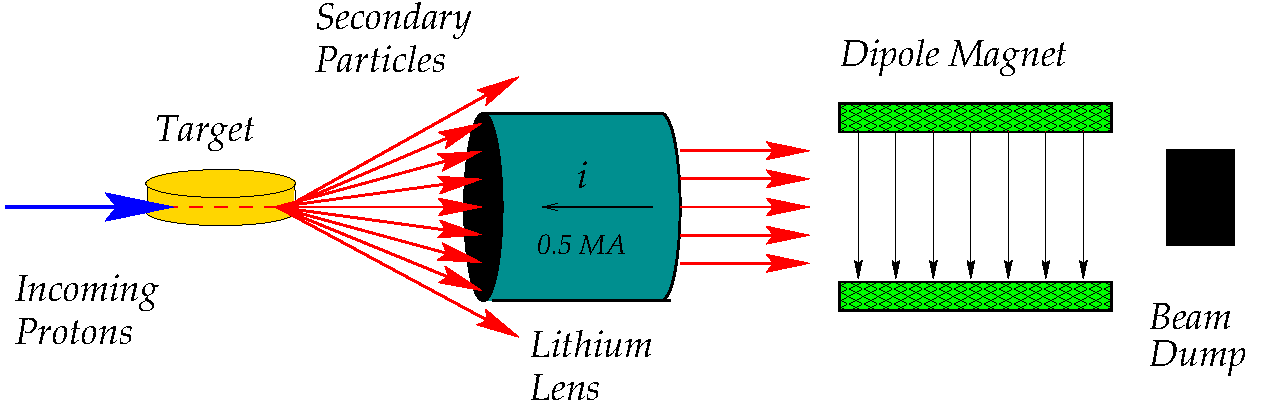
\includegraphics[scale=0.7,keepaspectratio=true,angle=0]{./Antiproton_production.pdf}
 % Antiproton_production.pdf: 255x779 pixel, 72dpi, 9.00x27.48 cm, bb=0 0 255 779
 \caption{Illustration of antiproton production. The dipole magnet directs the antiprotons to the Debuncher and other particles are sent to the beam dump.}
 \label{fig:AntiProtonProduction}
\end{figure}
\vspace{-0.03\textheight}

\subsection{Debuncher}
The Debuncher is a rounded-triangular synchrotron, and its primary purpose is to efficiently capture the antiprotons coming off the target, which have a very high momentum spread. The Debuncher does not accelerate the beam, but instead it helps to reduce the momentum spread. To accomplish this goal, it is equipped with a stochastic cooling system. In stochastic cooling, a signal is picked up from the circulating antiprotons at one side of the ring. That signal is amplified and sent directly across the ring. There, it is used to affect the trajectories of the antiprotons when they arrive. The Debuncher transfers the beam to the Accumulator, which holds the cooled antiprotons at 8~GeV until needed.

\subsection{Structure of Colliding Beams}
The Tevatron collides beams of protons and antiprotons with a center of mass energy of $\sqrt{s}=1.96$~TeV. The beam structure is the same for both protons and antiprotons. The Tevatron is operated with a radio frequency (RF) of 53.1~MHz which provides 18.8~ns long RF buckets. The nominal operation mode of the Tevatron in Run II has 36 bunches of protons and 36 bunches of antiprotons (36~$\times$ 36 mode). Each set of 36 bunches is distributed in three trains of 12 bunches each. The bunches in a train are separated by 21 RF buckets (or 396~ns). The trains are separated by a 139-bucket gap (2617~ns) called the abort gap. The 36~$\times$ 36 beam configuration is shown in Fig.~\ref{fig:BeamStructure}.

\begin{figure}[htbm]
 \centering
 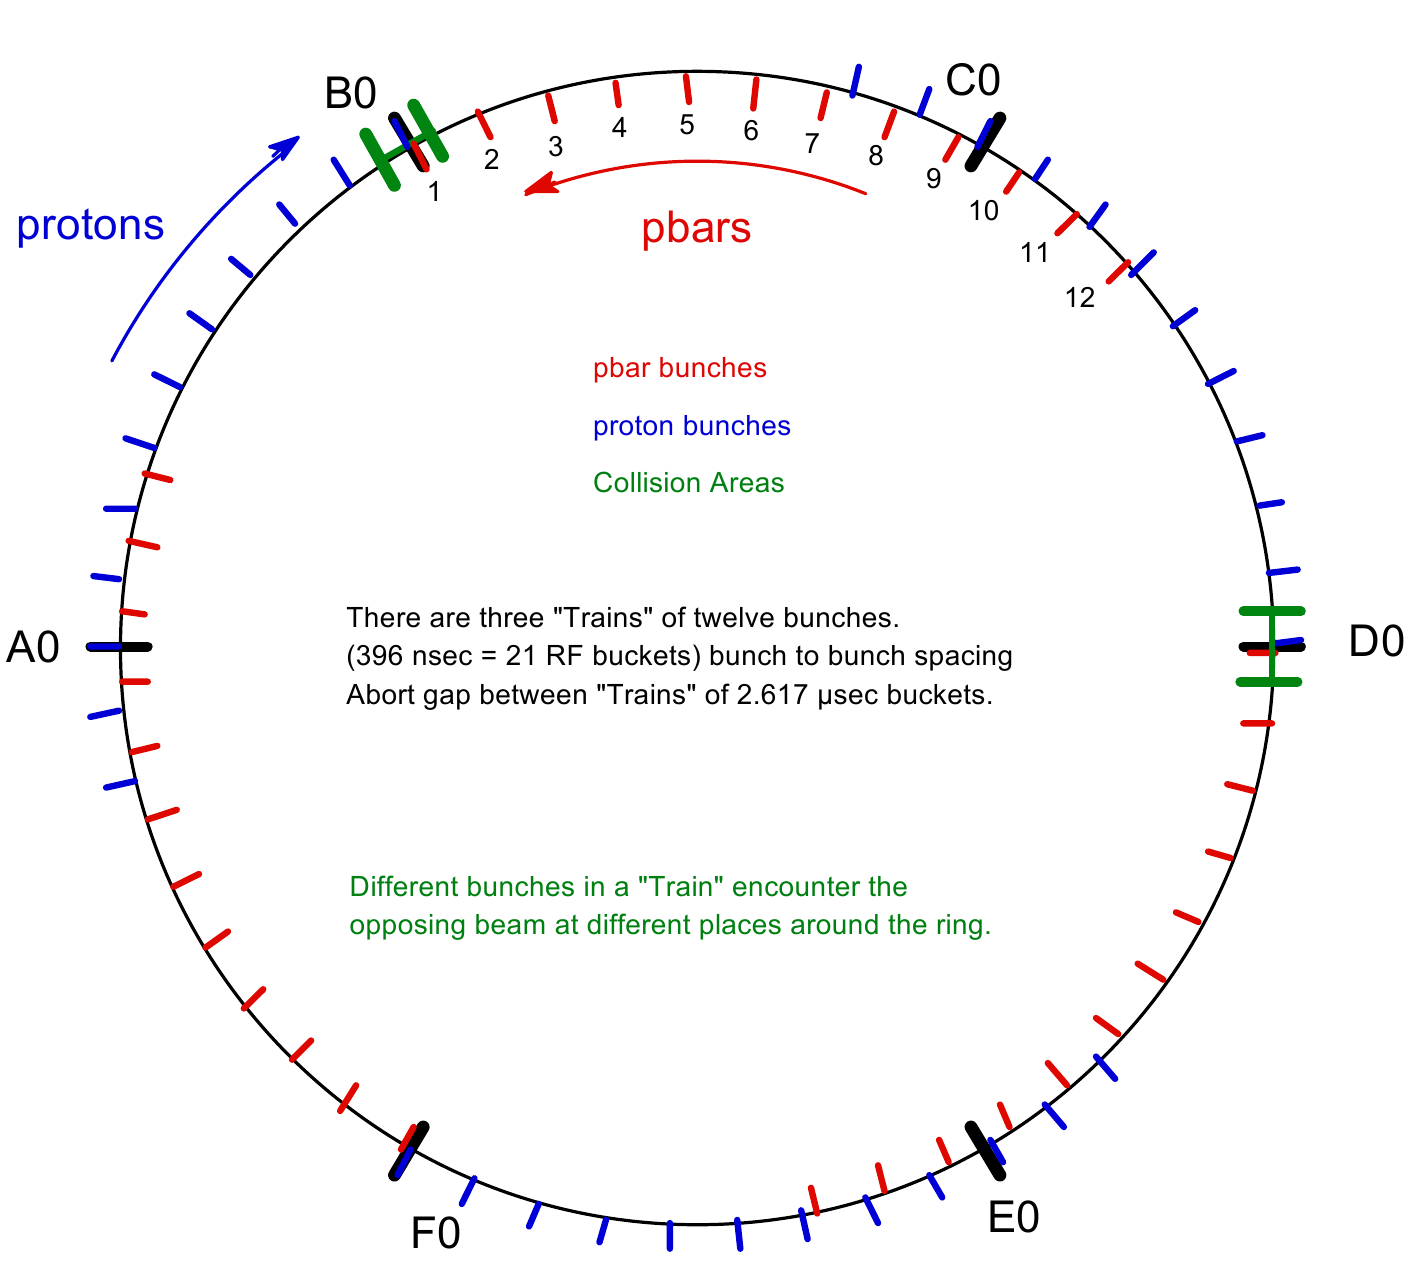
\includegraphics[scale=0.4,keepaspectratio=true]{./BunchStructure.png}
 % BunchStructure.png: 673x571 pixel, 96dpi, 17.80x15.11 cm, bb=0 0 505 428
\caption{Beam structure in 36~$\times$ 36 mode. Proton bunches go clockwise and are shown as blue marks outside the ring. Antiprotons go counterclockwise and are shown as red marks inside the ring. Detectors are located at B0 (CDF) and D0 (D\O).}
 \label{fig:BeamStructure}
\end{figure}
\vspace{-0.015\textheight}
If protons and antiprotons were orbiting in a central orbit as in Fig.~\ref{fig:BeamStructure}, the B0, D0 and F0 points would have the maximum number of collisions (12) per turn. However the present configuration is set to collide the beam at the two detectors (CDF and D\O) located at points B0 and D0. So any collisions produced at other points along the ring would be wasted. Any inefficiency is overcome by arranging the two beams into non-intersecting helical closed orbits. After the Tevatron ramps the beam energies to 980~GeV, the two beams are set in a collision helix. Several quadrupole magnets on either side of the CDF and D\O\ detectors squeeze and focus the beams to collide in the middle of the detectors.

\subsection{Instantaneous Luminosity ($\cal L$)}
Instantaneous luminosity (or simply luminosity) is a measure of the potential number of particle interactions for colliding beams. It depends on the intensity and phase space density of the interacting beams. The proton beam has about 10$^{13}$ particles and the antiproton beam has about 2$\times10^{12}$ particles. The two beams counterrotate in the accelerator ring.
%and have a Gaussian shape.
Each proton has a probability of interacting with an antiproton traveling in the opposite direction. The production rate for a specific type of interaction is defined by integrated luminosity (${\cal L}_{int}$) $\times$ cross section ($\sigma$), where the cross section is the measure of the probability for a specific type of interaction to occur in a proton-antiproton collision. Equation~\ref{eqa:LumDef1} shows the quantities used to calculate the luminosity.
\begin{equation}
{\cal L} = f \frac{N_{p}N_{\bar p}}{4\pi A}
\label{eqa:LumDef1}
\end{equation}
where $\cal L$ is the luminosity, $f$ is the frequency of bunch crossings, $N_{p}$ and $N_{\bar p}$ are the number of protons and antiprotons in each beam, and $A$ is the average size (area) of the transverse beam.

A high luminosity will yield a large interaction rate. From the above relationship, it is evident that the luminosity increases as the intensity per bunch increases and the cross sectional area of the bunch decreases. The performance of a collider is determined by integrating the luminosity over time ($\int{\cal L}~dt$). Since 2001, the Tevatron has delivered an integrated luminosity of about \cdfTotCurrLum with an ever-increasing rate (see Fig.~\ref{fig_CDFLumi}).

\section{The CDF Detector}
The Collider Detector at Fermilab (CDF) is a 5,000-ton general purpose detector with roughly 500,000 channels of information from various tracking and calorimeter components. The CDF detector is explained in detail elsewhere \cite{pap:CDFTDR, pap:CDFdetectorOverview}.

\begin{figure}[p!]
\begin{centering}
\subfigure[Integrated luminosity as function of the store number.]
{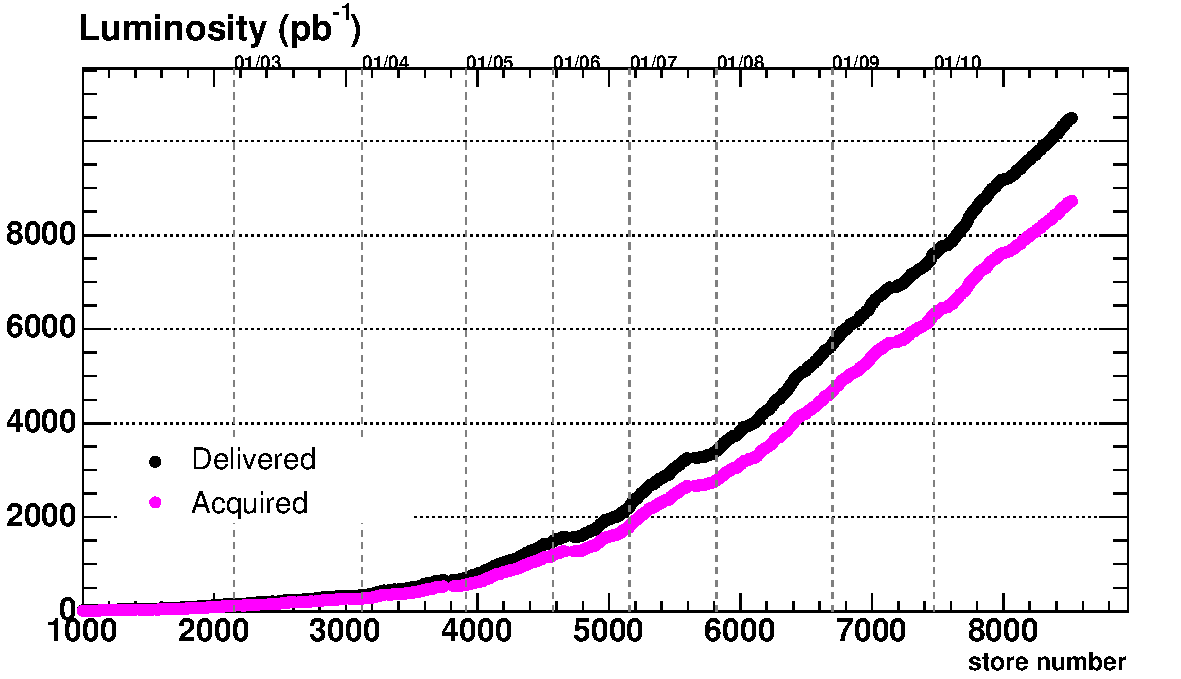
\includegraphics[scale=0.6]{CDFIntegratedLumi.pdf}
\label{subfig_lumInt}}

\subfigure[Peak instantaneous luminosity as a function of the store number.]
{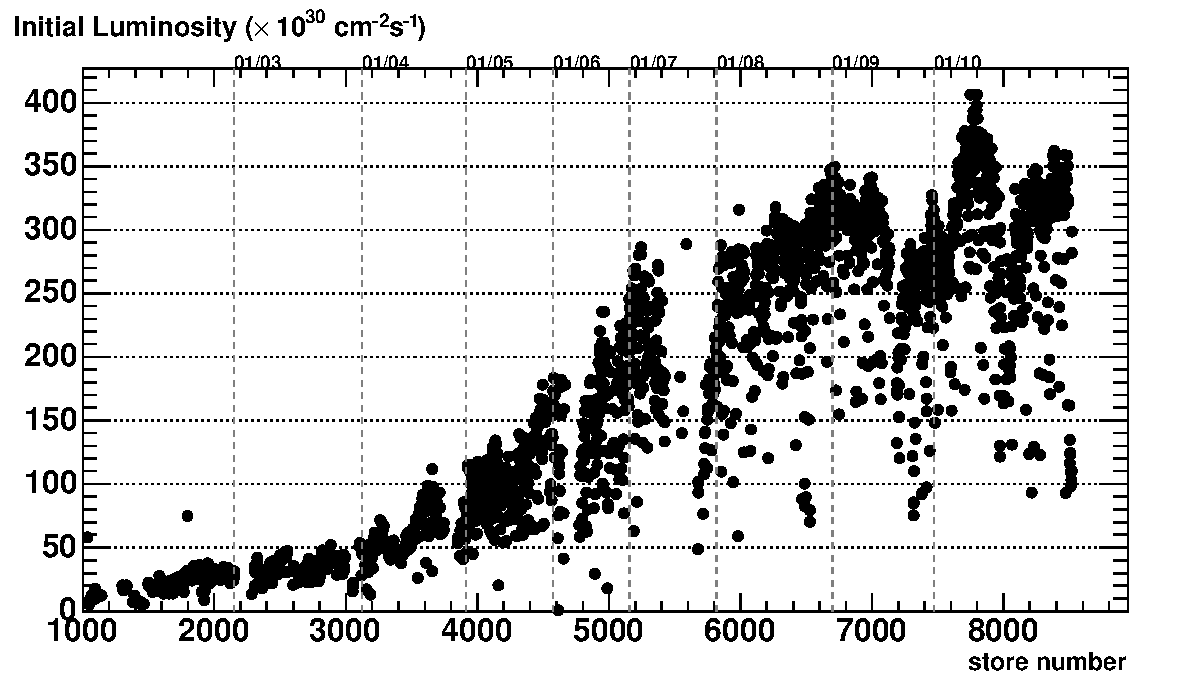
\includegraphics[scale=0.6]{CDFInitLum.pdf}
\label{subfig_lumInit}}

\caption{CDF luminosity measurements. (a) Integrated luminosity over time from 2002 to 2010 as a function of the store number, including both delivered luminosity and acquired luminosity (the amount that CDF was able to collect). This is a direct indication of the data-taking efficiency at CDF. (b) Peak instantaneous luminosity for each store over the same time period.}
\label{fig_CDFLumi}
\end{centering}
\end{figure}

At the time of writing this thesis, CDF has collected \cdfTotCurrLum~of data with a peak luminosity of around \mbox{300~$\times$ 10$^{32}$~\instLumUnits} (see Fig.~\ref{fig_CDFLumi}). A cutaway view of the CDF detector is shown in Fig.~\ref{fig_CDFdetCutAway}. The tracking system, comprised of a silicon pixel detector and open cell drift chamber, lies next to the beam pipe and is immersed in a superconducting solenoidal magnet. The amount and the direction of a deflected charged particle is used to infer its momentum and charge. Outside of the solenoid are the calorimeters, which measure the energy of particles produced in the collision. The muon detectors form the outermost layer of the CDF detector. Muons pass through the calorimeters and leave a signal in the muon chambers.

\begin{figure}[hbtm]
\begin{centering}
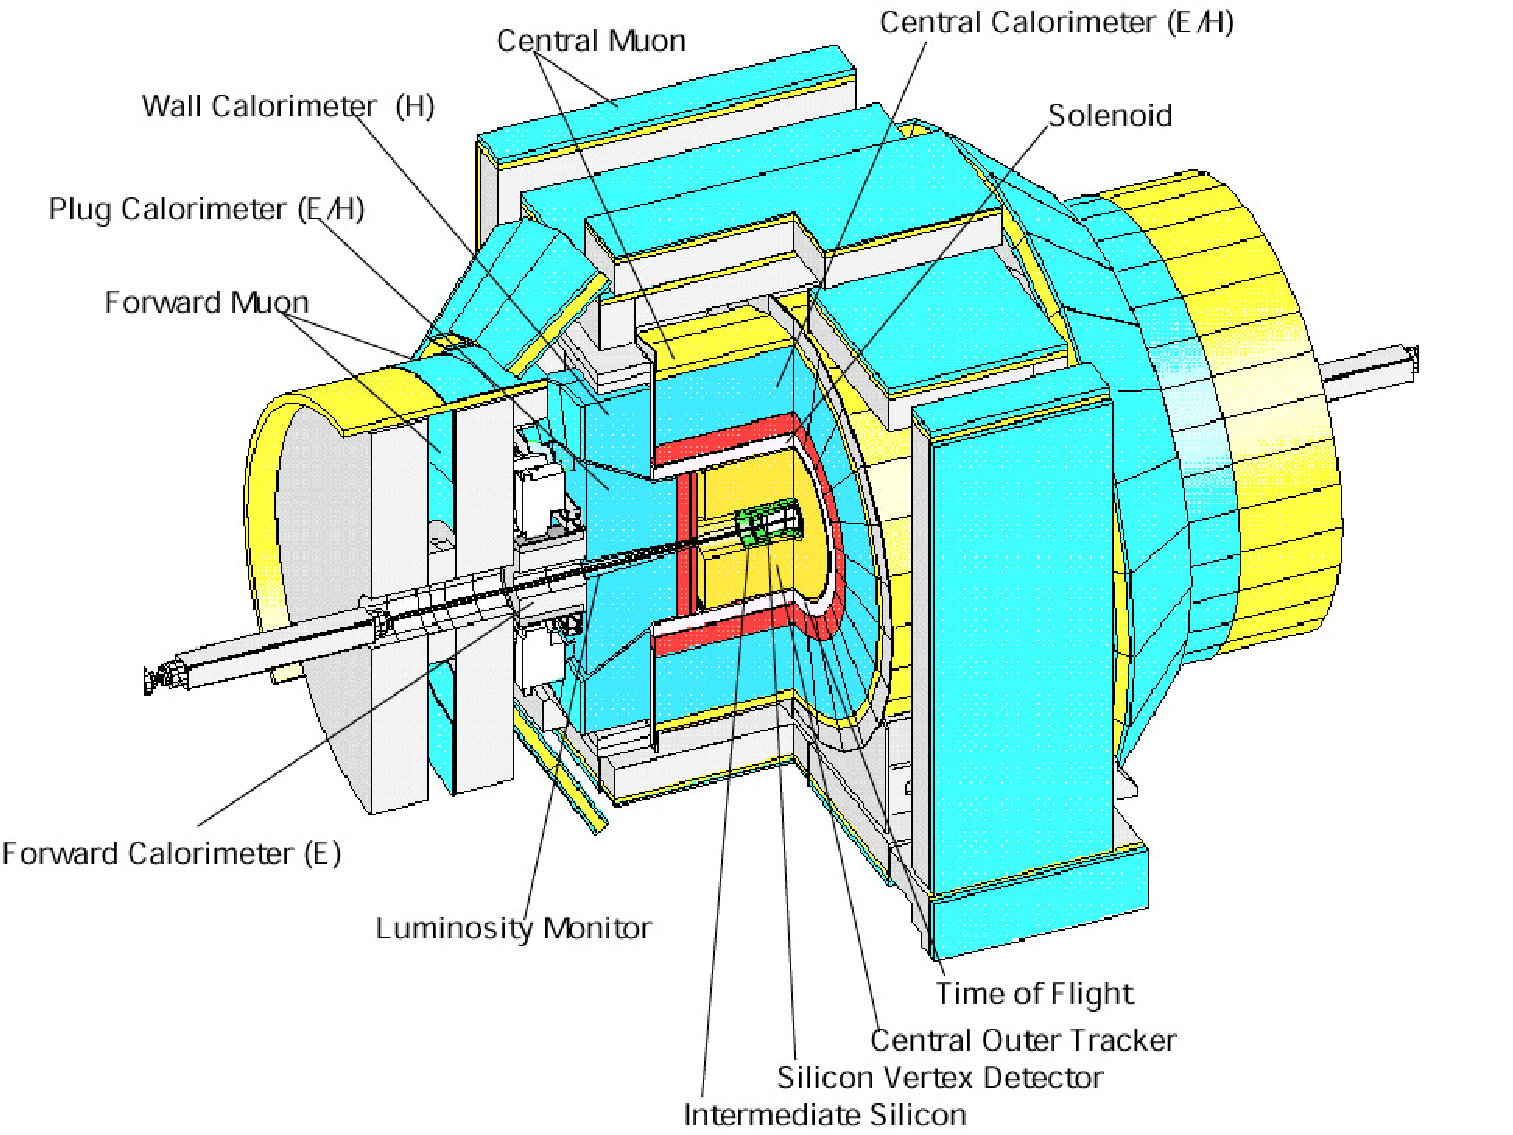
\includegraphics[scale=0.6]{CDFdetector_cutAwayView.pdf}
\caption{Cutaway view of the CDF detector.}
\label{fig_CDFdetCutAway}
\end{centering}
\end{figure}

The CDF detector is a combination of many subdetectors designed to detect certain properties of different particles and to completely reconstruct the collision event. Fig.~\ref{fig:particledecay} is a sketch of typical particle interactions in different subdetectors. The tracking chamber is the closest to the interaction point and the muon chamber is the furthest. All electrically-charged particles will leave trails in the tracking chamber. A photon, which has no electric charge, will not leave any mark in the tracking chamber but will deposit energy in the electromagnetic calorimeter. An electron is similar to a photon in the detector except that it will have an associated track. A muon, which is weakly interacting, has a longer mean lifetime than other leptons and escapes the detector leaving only a trail of hits along its path. A hadron, like the proton, will have a track and deposit the bulk of its energy in the hadron calorimeter. A neutral hadron like the neutron (\particle{n}), will show no tracks but deposit energy in the hadron calorimeter. The CDF detector exploits these simple distinctions to identify different particles and their properties.

\begin{figure}[htbm]
\begin{centering}
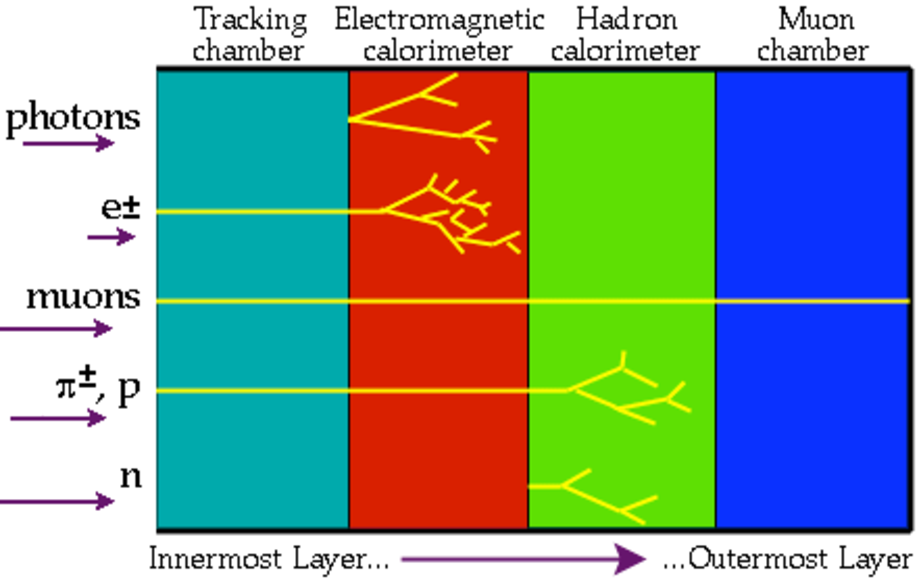
\includegraphics[scale=0.7]{decay_chart.pdf}
\caption{Diagram depicting particle interactions with different detectors. These differences help
to identify and distinguish particles generated in a hard scattering process.}
\label{fig:particledecay}
\end{centering}
\end{figure}

\subsection{Coordinate System}
The coordinate system used to describe the location of different components in the CDF detector is illustrated in Fig.~\ref{fig:cdfCDTsystem} and described below.

\begin{figure}[htbm]
 \centering
 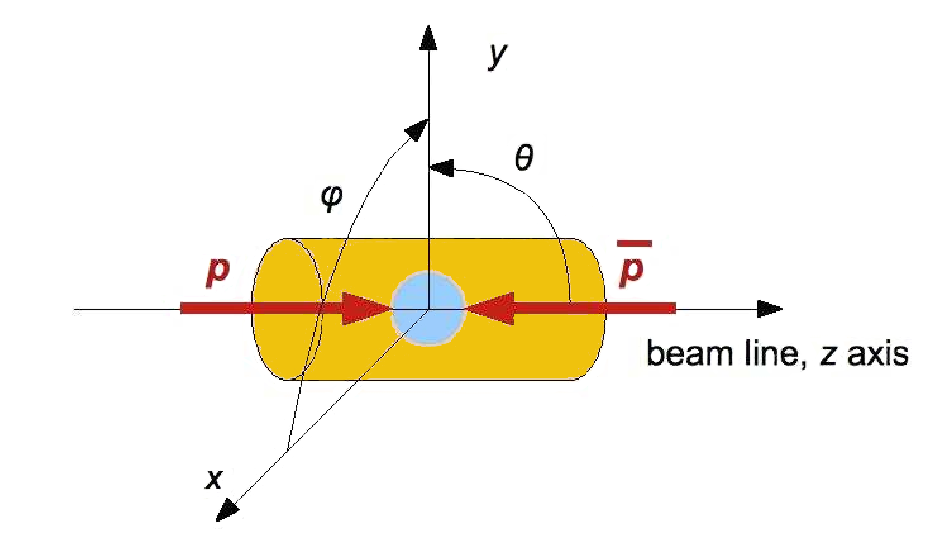
\includegraphics[scale=.5]{./cdfCoordinateSystem.png}
 % cdfCoordinateSystem.png: 937x550 pixel, 96dpi, 24.79x14.55 cm, bb=0 0 703 412
 \caption{CDF coordinate system.}
 \label{fig:cdfCDTsystem}
\end{figure}

\vspace{-0.015\textheight}
\begin{singlespace}
\begin{itemize}{}{}
\item{$z$ = Distance along the beamline. Protons travel in the $+z$ direction (east) and antiprotons travel in the $-z$ direction (west). $z=0$ is the interaction point (IP).}
\item{$r$ = Radial distance from the beamline.}
\item{$\theta$ = Polar angle from the beamline. \mbox{$\theta$ = 0\degree} is the $+z$ direction, \mbox{$\theta$ = 90\degree} is straight up, and \mbox{$\theta$ = 180\degree} is the $-z$ direction. Typically $\eta$, as described below, is used instead of $\theta$.}
\item{$\eta$ = Pseudorapidity, which is defined as $-\ln(\tan(\theta/2))$, so particles perpendicular to the beamline have $\eta = 0$. The beamline itself has an $\eta$ of $+\infty$ in the $+z$ direction and $-\infty$ in the $-z$ direction. \mbox{$\theta$ = $\pm$45\degree} corresponds to \mbox{$\eta=\pm$0.88}.}
\item{$\phi$ = Azimuthal angle around the beamline. North is \mbox{$\phi$ = 0}, up is \mbox{$\phi$ = 90\degree}, south is \mbox{$\phi$ = 180\degree}, and down is \mbox{$\phi$ = 270\degree}.}
\end{itemize}
\end{singlespace}

The CDF detector is left-right and cylindrically symmetric with few exceptions. Many components in the CDF detector are segmented into \mbox{15-degree} wedges in $\phi$. These wedges are numbered with 0 at \mbox{$\phi$=0}, proceeding in the \mbox{+$\phi$} direction. Usually, a wedge refers to a given $\phi$ segment on a given east/west side of the detector; for example, wedge 0E refers to the wedge from \mbox{0--15} degrees $\phi$ on the east side of the detector, and wedge 0W refers to the wedge from \mbox{0--15} degrees $\phi$ on the west side of the detector. The CDF detector is further classified into three regions of pseudorapidity, \newterm{central} (\etalessthan{1.1}), \newterm{plug} (\etaabsregion{1.1}{3.6}), and \newterm{forward} ($|\eta|>3.6$). Figure \ref{fig:EtaRegionsTowerGeometry} shows a schematic view of a quarter of the CDF detector. It shows the projective tower geometry and the relative location of the subdetectors.

\begin{figure}[htb!]
 \centering
 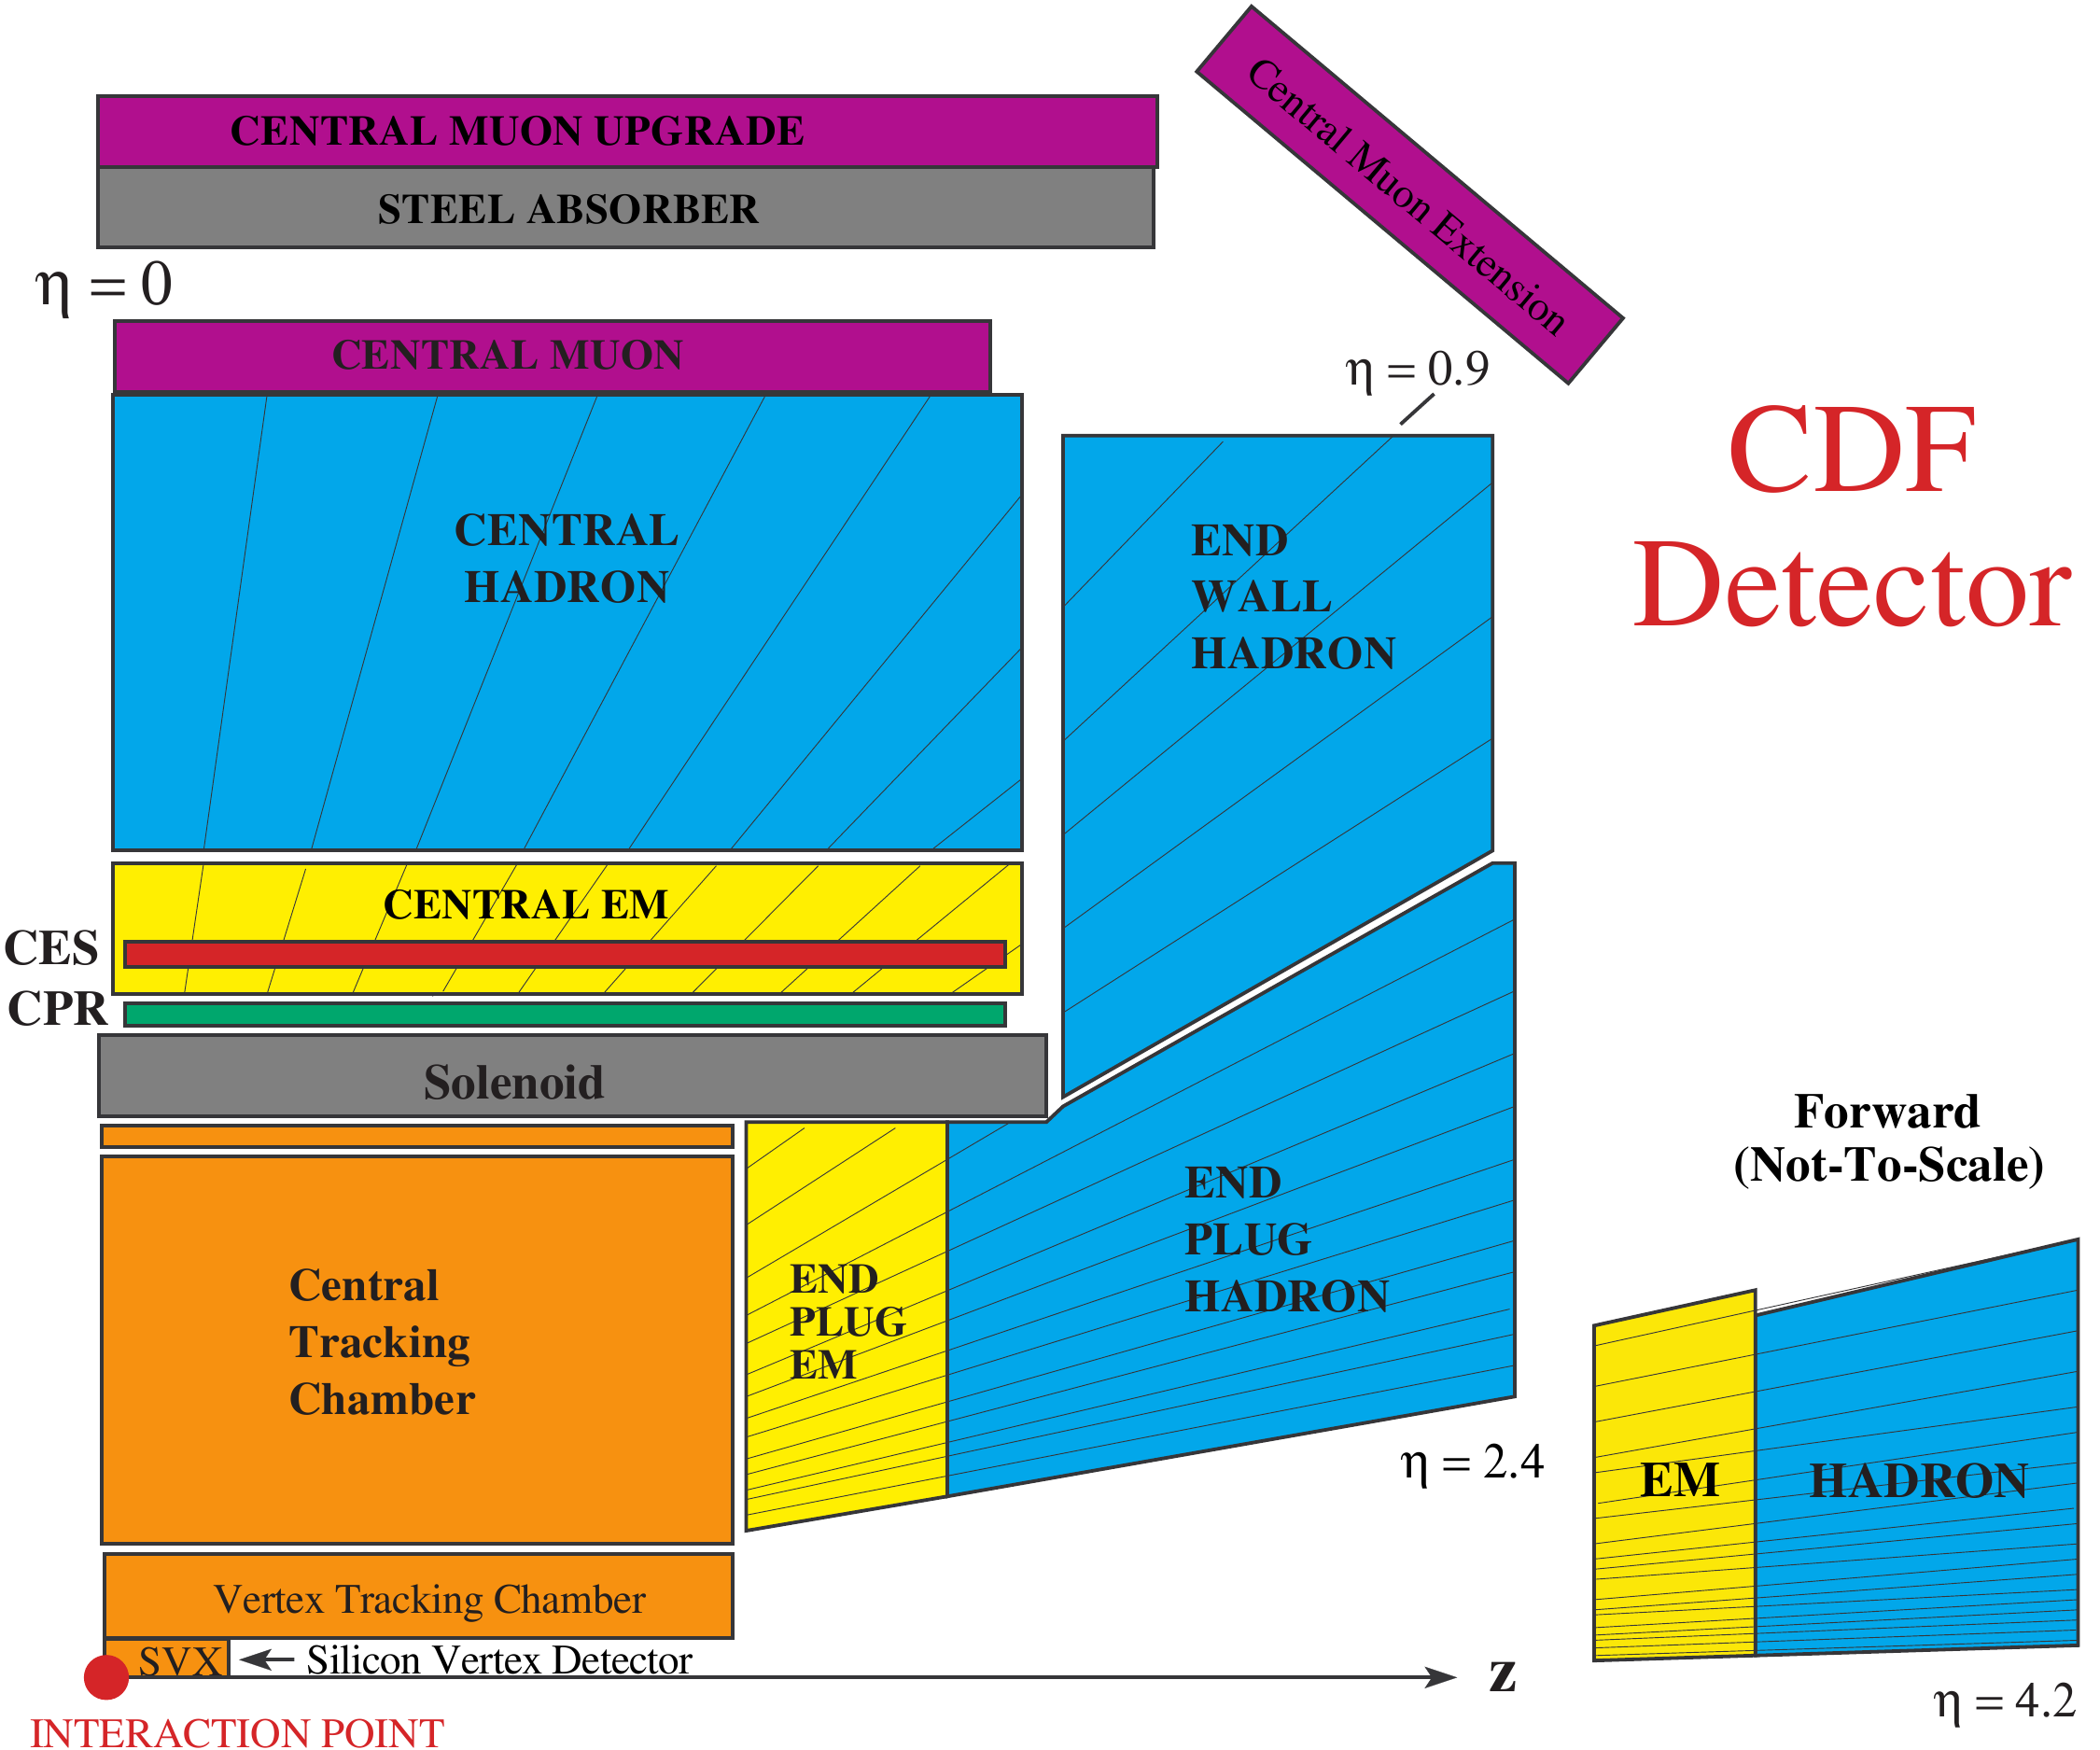
\includegraphics[scale=0.24]{./CDF_ColorQuarter_TowerGeometry.png}
 % CDF_ColorQuarter_TowerGeometry.png: 2250x1875 pixel, 96dpi, 59.52x49.60 cm, bb=0 0 1687 1406
 \caption{A quarter view of the CDF detector indicating the location of different subdetectors with respect to the nominal collision (interaction) point. $\eta$-regions and the projective tower geometry are indicated by lines extending from the interaction point.}
 \label{fig:EtaRegionsTowerGeometry}
\end{figure}


\subsection{Luminosity Counter}
The CDF detector is equipped with high-yield gaseous Cherenkov counters for precise measurement of the luminosity. Located close to the beamline (\etaabsregion{3.7}{4.7}), it measures the Cherenkov radiation (light) from the inelastic collisions (see Fig.~\ref{fig_CLC_Assembly}). The light measured is proportional to the number of inelastic collisions \cite{pap:CLCperformance}. The luminosity can be calculated using
\begin{equation}
%\lum \mathrm{= \frac{\mu \times f_{BC}} {\sigma _{in}} }
{\cal L} = \frac{\mu \cdot f_\mathrm{BC}}{\sigma_{\mathrm{in}}},
\label{eqa:LumDef2}
\end{equation}
where $\cal L$ is the instantaneous luminosity, $f_\mathrm{BC}$ is the rate of bunch crossings (1.7~MHz), $\mu$ is the average number of \ppbar interactions per bunch crossing, and $\sigma_\mathrm{in}$ is the inelastic cross section (=~60~mb).


\begin{figure}[htb!]
\begin{centering}
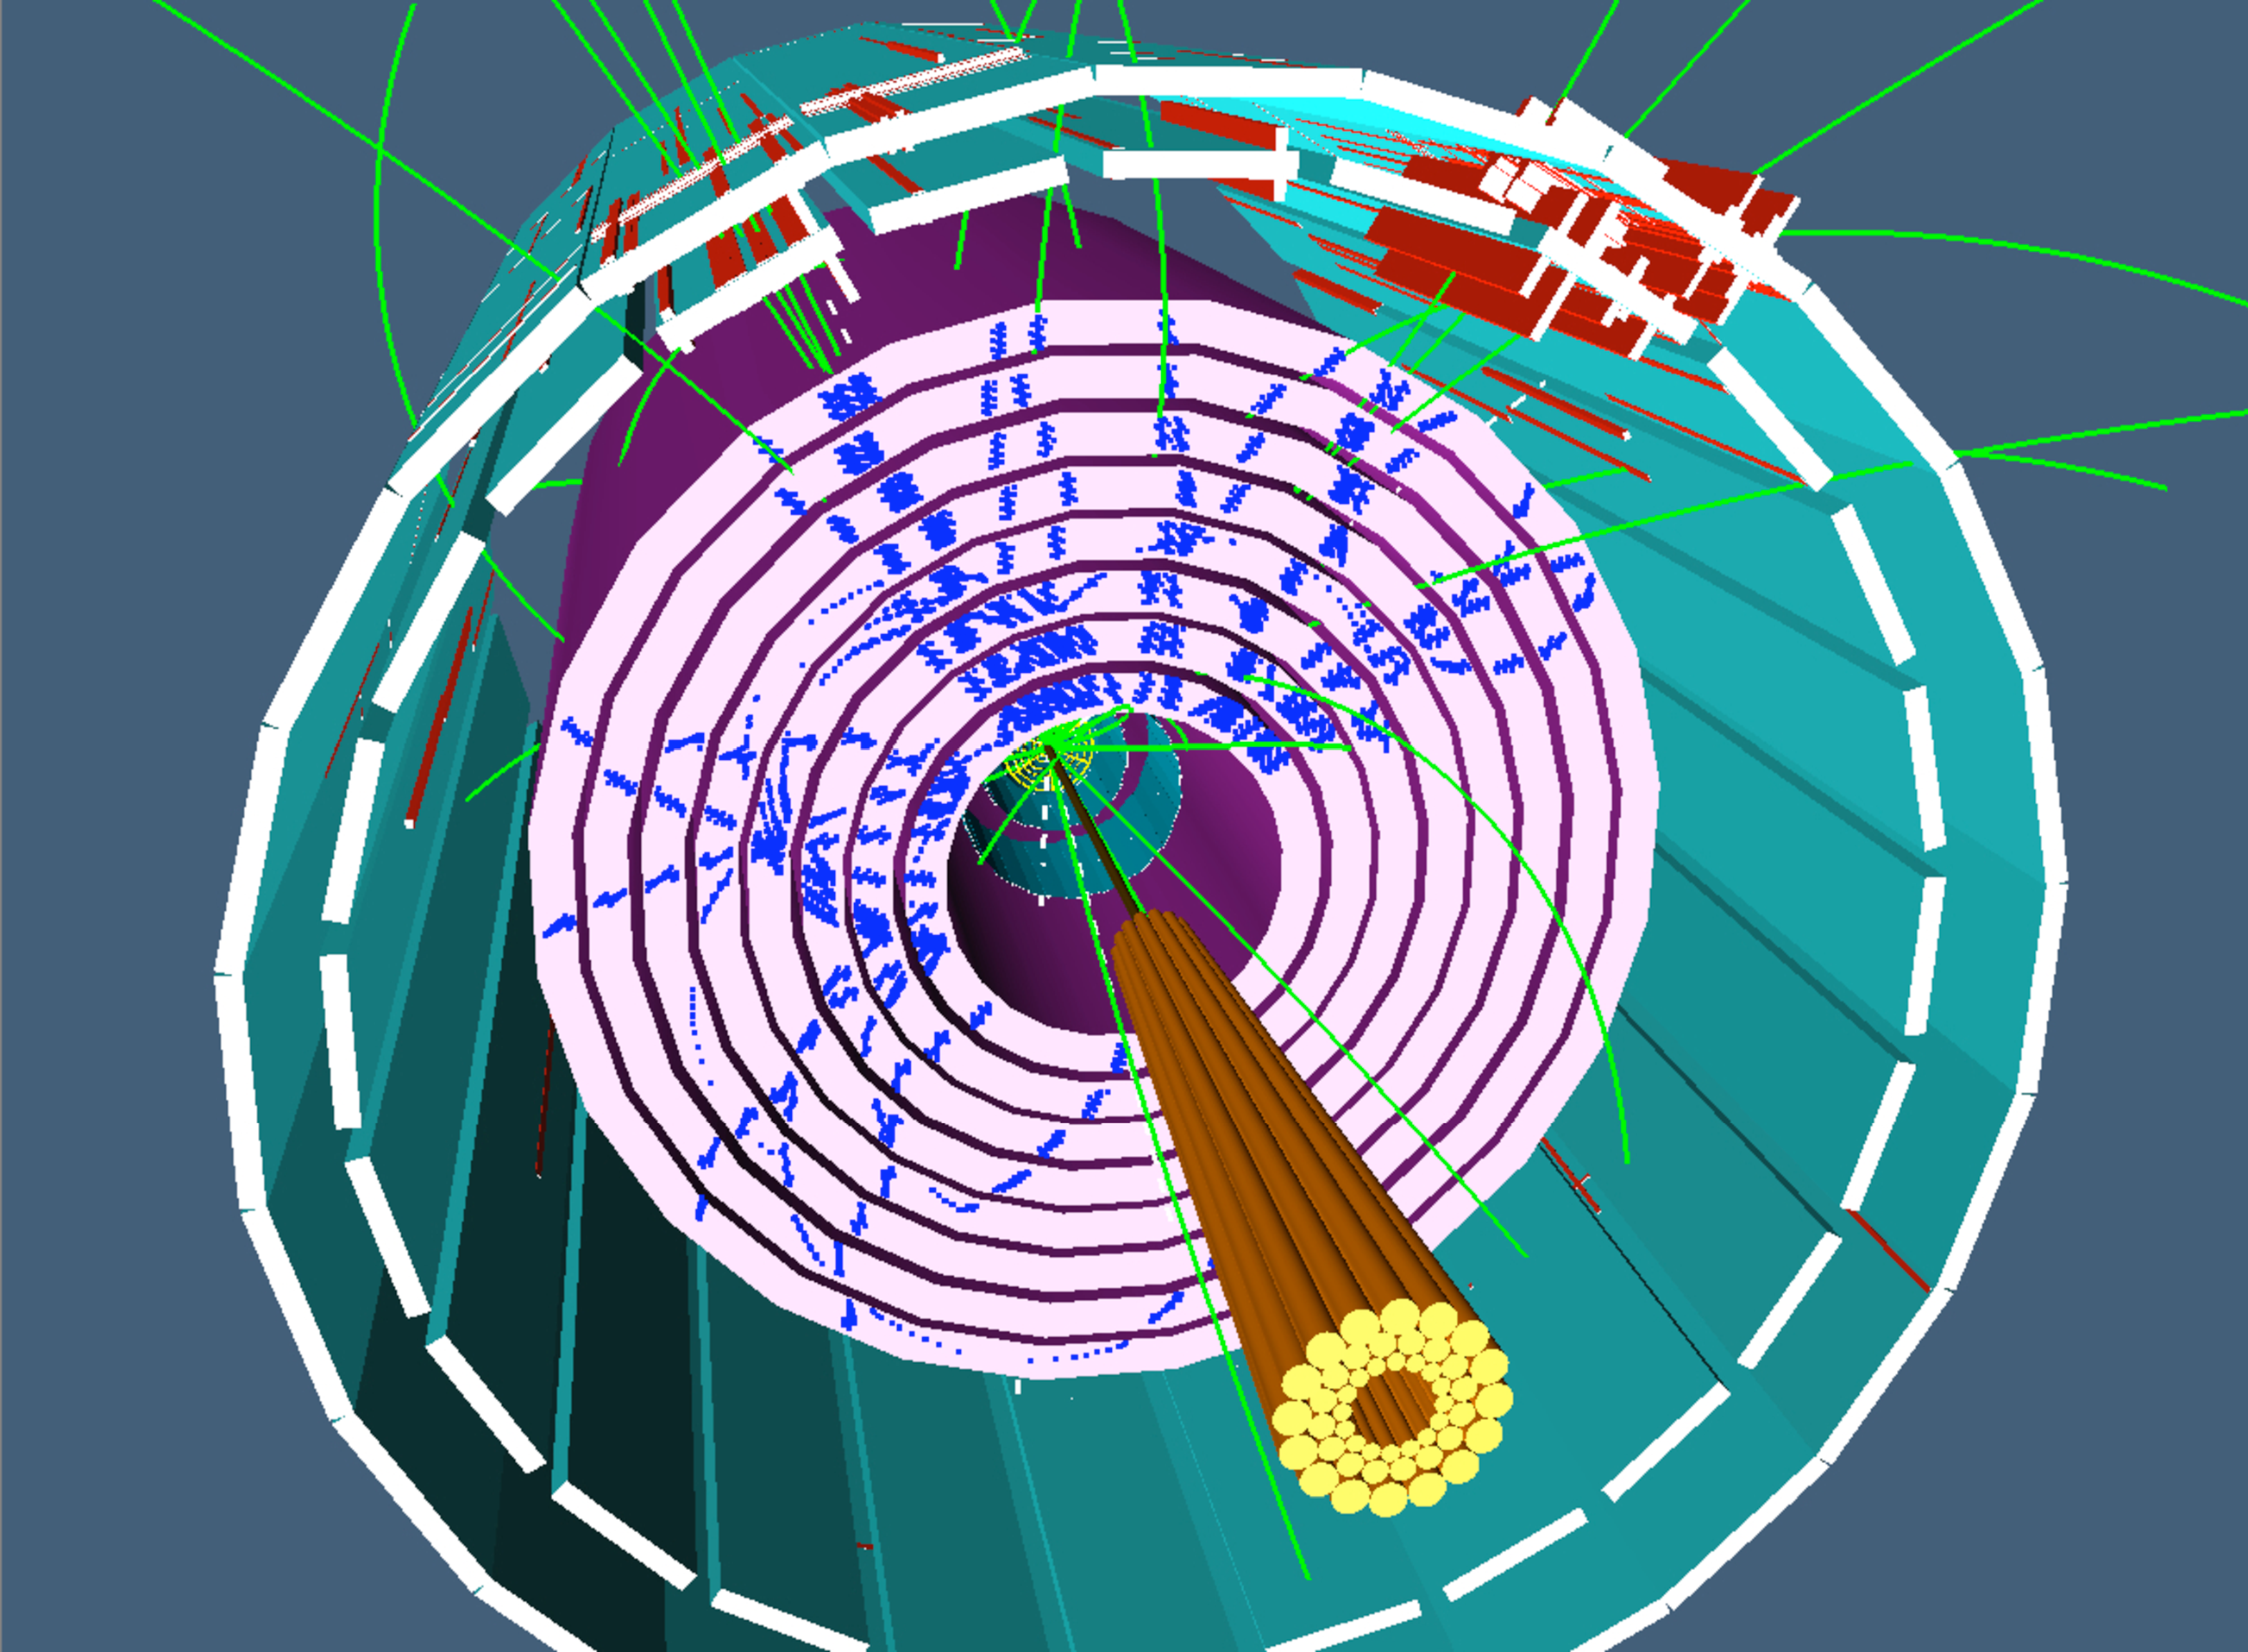
\includegraphics[scale=0.3]{CLC_withTracks.pdf}
\caption{Graphic depicting the CLC detector (in brown).}
\label{fig_CLC_Assembly}
\end{centering}
\end{figure}


\subsection{Solenoid}
The CDF tracking volume is immersed in a 1.4~T magnetic field generated by a 5~m long Nb-Ti superconducting solenoid. The magnetic field is aligned along the direction of the beam pipe so it does not deflect the protons or antiprotons circling in the Tevatron. Secondary particles from the collisions traveling perpendicular to the beam pipe are deflected by the magnetic field according to the Lorentz force law, $\vec{F}=q\vec{v}\times \vec{B}$. This allows the tracking detectors to measure the momenta of particles and the sign of their charge.

\subsection{Tracking System}\label{sec:TrackingSystem}
A well equipped high-precision charged-particle tracking system is used at CDF. It is comprised of an open cell drift chamber, the Central Outer Tracker (COT), and a set of silicon layers laid inside the COT close to the beam pipe (see Fig.~\ref{fig:TrackingCoverage}). A micro-vertex detector close to the beam pipe measures the impact parameter resolution. A set of intermediate silicon strips enhances the vertex and track reconstruction. The silicon strips, when combined with the COT tracks, increase the \pt resolution and are used for $b$-tagging in the forward region. When used alone, the silicon detector provides tracking over the full region of \mbox{$|\eta|\leq2.0$}. This state-of-the-art tracking system is at the heart of many analyses performed at CDF.

\begin{figure}[htb!]
\begin{centering}
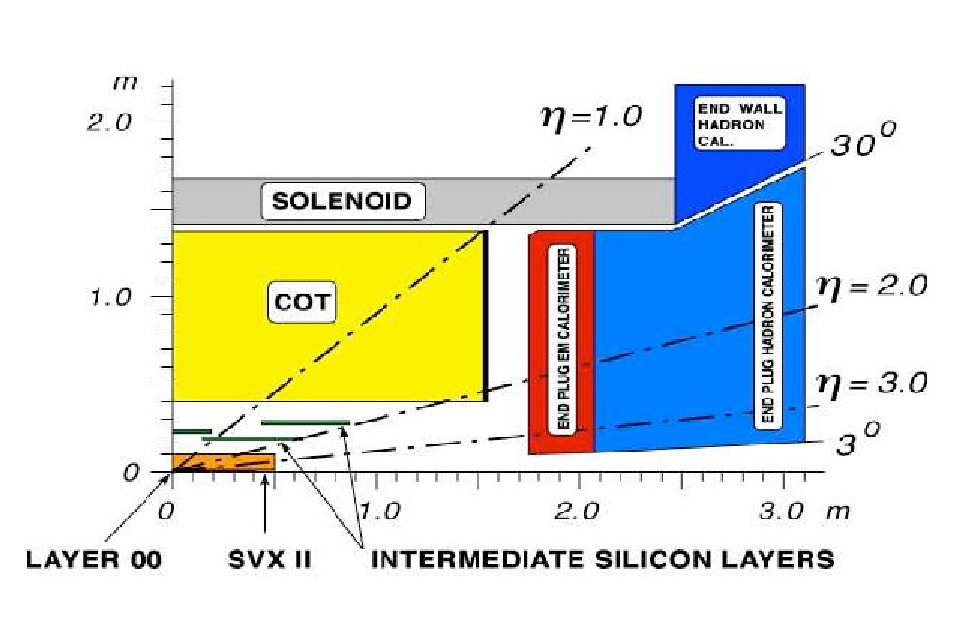
\includegraphics[scale=0.95]{CDF_TrackingCoverage.pdf}
\caption{Tracking coverage of the CDF detector. The figure only shows 1/4 of the detector. The nominal collision point is at coordinate (0,0).
}
\label{fig:TrackingCoverage}
\end{centering}
\end{figure}

\subsubsection{Silicon Tracking}\label{sec:SiliconTracking}
Nine layers of silicon micro strips measure the $x$, $y$ and $z$ positions of the charged particles produced in a collision \cite{pap:SiliconDetector}. They lie next to the beam pipe and comprise 3 detector subsystems. The first silicon layer, Layer 00 (L00), is mounted on the beampipe. The next five silicon layers make up the Silicon Vertex Detector (SVX-II) (Fig.~\ref{fig_SvxEndView}). And the last three make up the Intermediate Silicon Layers (ISL) which cover the region \etalessthan{2}. The L00 detector enhances the vertex and tracking capabilities and has a 11~micron hit resolution. The main purpose of the SVX-II is high-precision tracking and secondary vertex detection. The SVX-II has a position resolution of $\sim$9 microns for 2-strip clusters. The SVX-II and ISL together provide stand-alone silicon tracking and are vital for $b$-tagging. The single hit resolution is \mbox{$\leq16~\mu m$} on the axial side and $\leq$~23~$\mu$m on the stereo side. The silicon system's impact parameter resolution is approximately 40~$\mu$m.

\begin{figure}[htb!]
\begin{centering}
\raisebox{0.25\height}{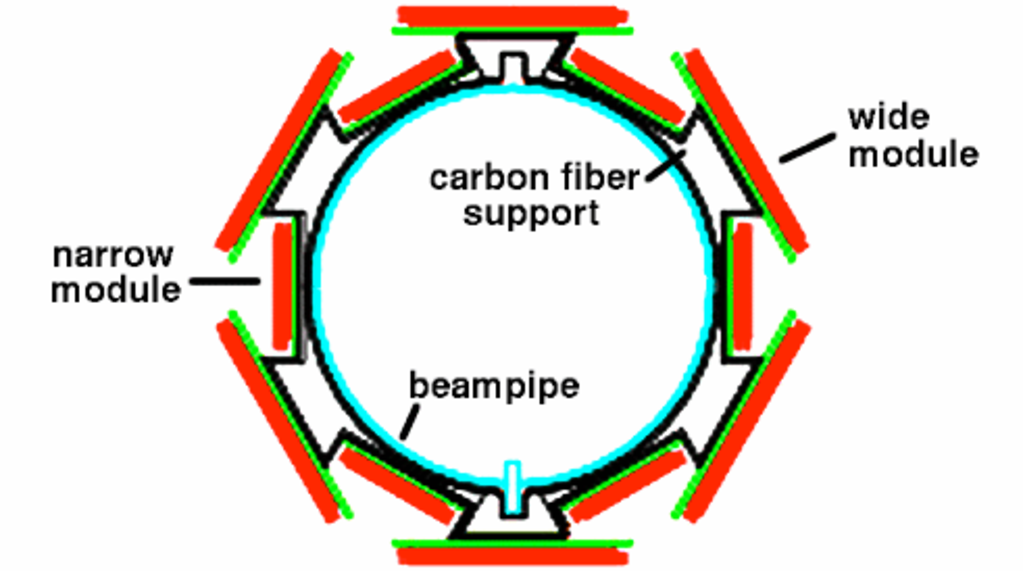
\includegraphics[scale=0.4]{L00EndView.pdf}}
\hspace*{.2in}
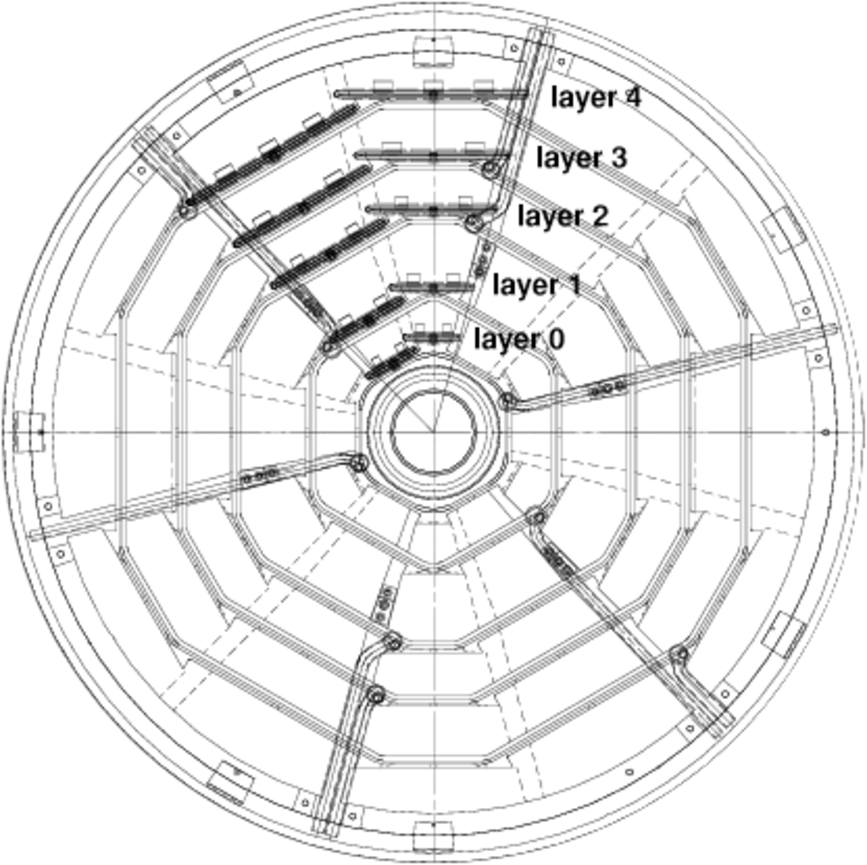
\includegraphics[scale=0.4]{SvxBulkHeadEndView.pdf}
\caption{End view of the Layer 00 silicon detector (left), and end view of the SVX-II silicon vertex detector (right).}
\label{fig_SvxEndView}
\end{centering}
\end{figure}

\subsubsection{Central Outer Tracker (COT)}\label{sec:COT}
The COT \cite{pap:COT} is an open cell drift chamber providing complete charge particle tracking coverage over the region \mbox{$|\eta|\leq1.0$} and partial coverage up to \etalessthan{2}. It has a inner radius of \mbox{44 cm}, a outer radius of \mbox{132 cm}, and spans about 3~m in length along the beamline ($z$). The complete chamber is roughly 1.3\% of a radiation length at normal incidence. A total of 2520 cells called \newterm{supercells} are arranged to form 8 layers called \newterm{superlayers} (SL) to reconstruct tracks with high precision and purity. Cells across layers are designed to have approximately the same maximum drift distance, and the number of cells increases with radius as seen in Fig.~\ref{fig:COT_endview}. Cells are filled with fast-response ionizing gas which limits drift times to less than 100~ns. A drift cell has a line of 12 sense wires and 12 shaper wires placed alternatively in the middle of the cell (Fig.~\ref{fig:COT_cells}). The superlayers are arranged in alternating \newterm{axial} and \newterm{stereo} layers. Axial super layers have the wires in the cells running parallel to the $z$ axis. Wires in the stereo layers are shifted by a 3\degree angle with respect to the $z$ axis. This provides an apparent shift in the charge particle track to give a 3-dimensional view of the tracks. The combination of axial and stereo layer information provides the $z$ and $r-\phi$ positions.

\begin{figure}[htb!]
 \centering
 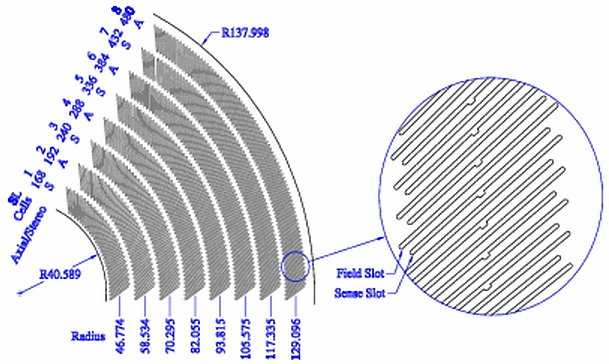
\includegraphics[keepaspectratio=true,scale=0.6]{./cot_end.png}
 % cot_end.png: 609x364 pixel, 72dpi, 21.48x12.84 cm, bb=0 0 609 364
 \caption{A section of 1/6 of the COT end plate. The information given for each superlayer is the total number of supercells, the wire orientation (axial or stereo), and the average radius in centimeters. The enlargement shows the sense and field slot geometry in detail.}
 \label{fig:COT_endview}
\end{figure}

\begin{figure}[htb!]
 \centering
 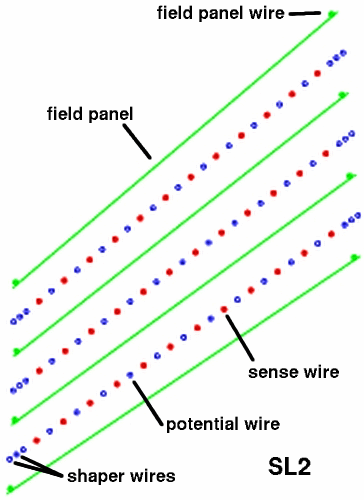
\includegraphics[keepaspectratio=true,scale=0.8]{./cot_cells.png}
 % cot_cells.png: 364x500 pixel, 72dpi, 12.84x17.64 cm, bb=0 0 364 500
 \caption{Three COT cells in superlayer 2 looking down along the beamline, $z$. Note that some details are not to drawn to correct scale.}
 \label{fig:COT_cells}
\end{figure}

% Table not complete ##############################
% SEE Nucl. Inst. Meth A 42586
% \begin{table}
% \centering
% \begin{tabular}{cc}
% \hline
% {\bf } & {\bf Momentum Resolution $\sigma(p_{T})/p_{T})$}\\
% \hline
% COT alone & 0.15\% |\\
% \end{tabular}
% \caption{Momentum resolution when COT and Silicon tracking systems are combined.}
% \label{tab:COTMomentumResolution}
% \end{table}

\subsection{Preshower Detector}\label{sec:CPR}
The preshower detector is used to sample the particles before they reach the calorimeter. As there is lot of material (the COT, the magnet) in between the calorimeter and the interaction point, particles such as photons can convert in material (for example, $\gamma\to e^{+}+e^{-}$). The preshower detector acts as a redundant measurement for particle identification. In Run II, the gas-filled preshower detector was replaced with a fast-response low-noise scintillator tile detector (see Fig.~\ref{fig:CPRtile}). Unlike the old detector, the new detector has no dead regions. A continuous array of 3~$\times$ 18 tiles (12.5~$\times$~12.5~cm$^2$ each) spans the face of one calorimeter wedge. It samples the early particle shower in front of the central calorimeter (see Fig.~\ref{fig_cprlocation}). The preshower detector can be used to efficiently identify single photons from light meson decays (\textit{e.g.} $\pi^{0}\rightarrow\gamma\gamma$) to improve photon measurements \cite{pap:CPRdetector}. Above 35~GeV, photons from light meson decays cannot be resolved using only the shower maximum detector (see Section~\ref{sec:CES}) because the angular separation of the two photons is too small. This new scintillator detector is designed to measure single particles and requires more then 5 photo electrons per minimum ionization particle (MIP).

\begin{figure}[htb!]
 \centering
 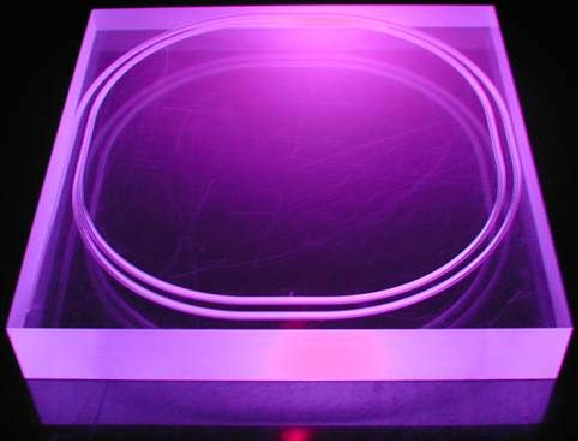
\includegraphics[scale=.5]{./CPRtile.png}
 % CPRtile.png: 578x441 pixel, 96dpi, 15.29x11.67 cm, bb=0 0 433 331
 \caption{A scintillator tile used in the new preshower detector. The tile is carved with a two-loop spiral groove in which a wavelength-shifting (WLS) fiber is embedded. The fiber carries out the light produced by the tile.}
 \label{fig:CPRtile}
\end{figure}


\begin{figure}[htb!]
\begin{centering}
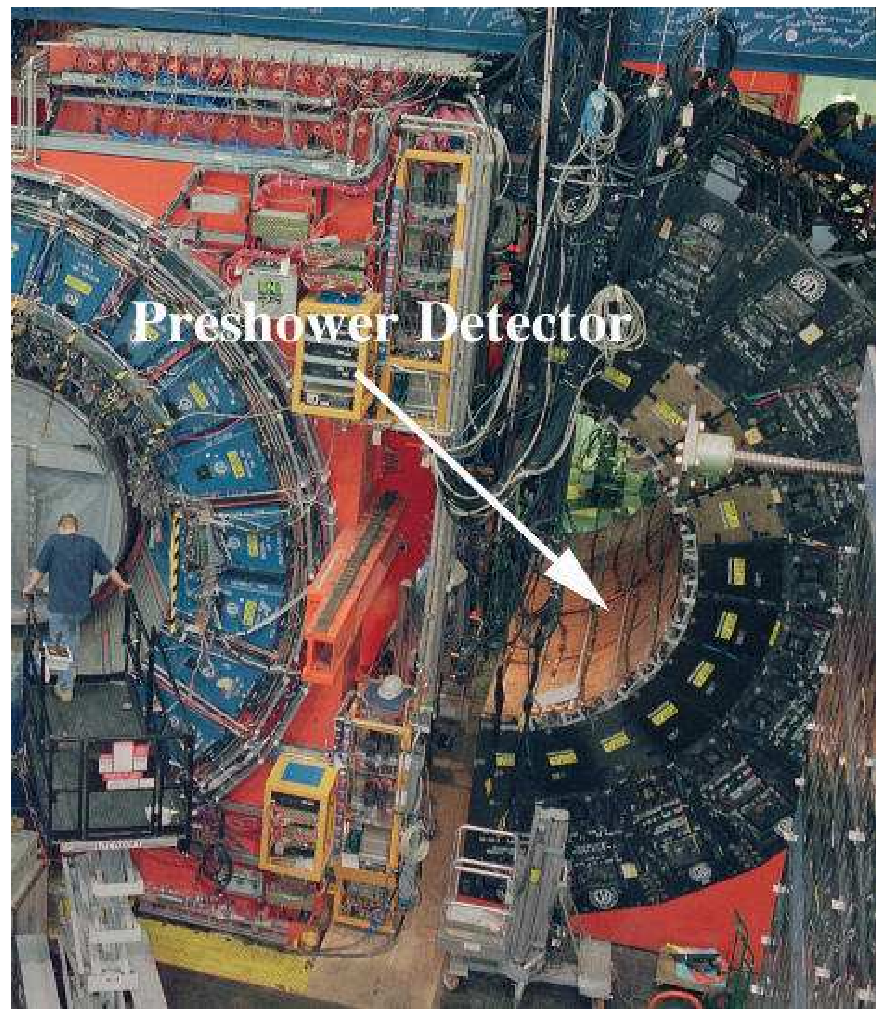
\includegraphics[scale=0.35]{CPR_Location2.png}
\caption{Photo of a section of the CDF detector before the new preshower detector installation. One of the calorimeter arches is open for maintenance, and twelve calorimeter wedges are visible. On the inner surface of each of the calorimeter wedge lies an array of scintillator tiles for the preshower detector.}
\label{fig_cprlocation}
\end{centering}
\end{figure}

\begin{figure}[htb!]
 \centering
 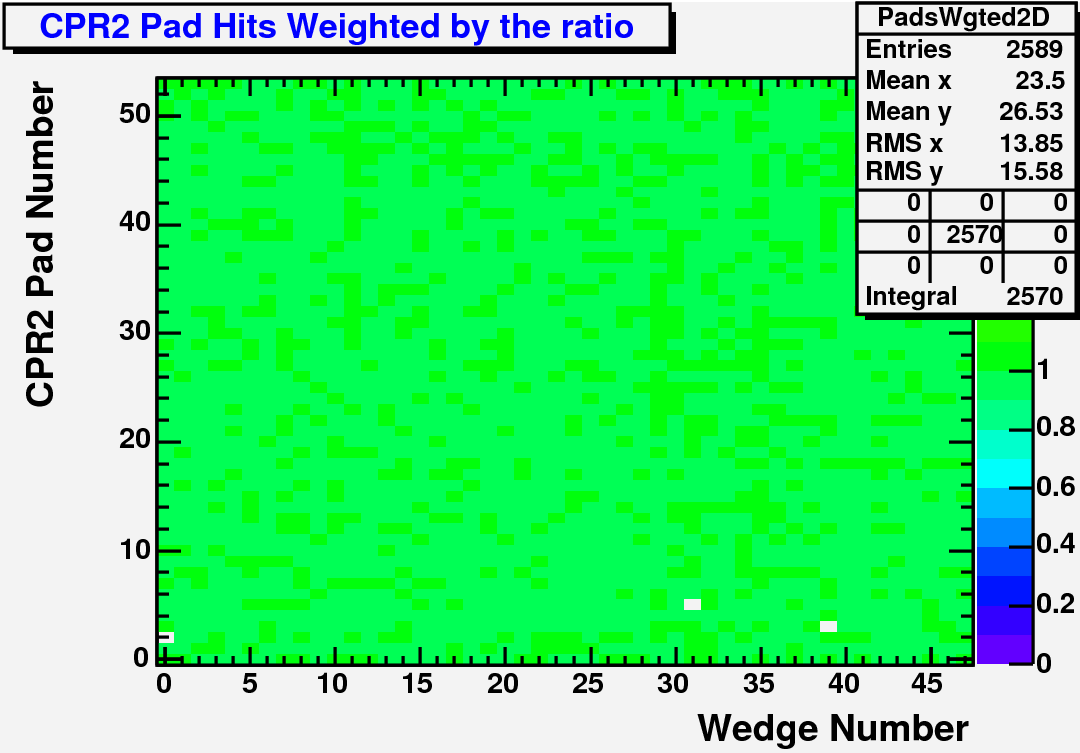
\includegraphics[scale=0.35,keepaspectratio=true]{./CPRcalibration1.png}
 % CPRcalibration1.png: 1080x753 pixel, 96dpi, 28.57x19.92 cm, bb=0 0 810 565
 \caption{A histogram used in the calibration process to check the energy gain of CPR tiles. The \newterm{dead} channels show up in white. Each tile's gain is compared to the global response, and tiles with low gain will show up in warm colors.}
 \label{fig:CPRcalibration}
\end{figure}

The author was part of the offline calibration group that provided calibration information on the CPR detector. Due to radiation damage and aging of the scintillator tiles, their photoproduction diminishes over time and the response to MIPs needs to reevaluated. For this, every CPR channel's gain is adjusted for each run period. A sample calibration plot of the CPR detector is shown in Fig.~\ref{fig:CPRcalibration}. Furthermore, the CPR detector status (whether it was on and functioning properly during data-taking) was determined by measuring the occupancy and reported to the Data Quality Monitoring (DQM) group. This information is used to determine whether certain data is useful for physics analysis (see Section~\ref{sec:GoodRun}).

\subsection{Calorimeter System}\label{sec:Calorimeter}
The calorimeter system is located outside of the solenoid and it is a tower-segmented scintillator sampling calorimeter. The calorimeter has a projective tower geometry (see Fig.~\ref{fig:EtaRegionsTowerGeometry}) where each tower is 15\degree in azimuth by about 0.11 in pseudorapidity. Each wedge consists of a lead-scintillator electromagnetic calorimeter section backed by a steel-scintillator hadron calorimeter \cite{pap:CDFTDR}. The central calorimeter system extends to \etaregion{-1.1}{1.1} and the plug calorimeter to \etaabsregion{1.1}{3.6}. Calorimeter information is read out via mounted fast PMTs. The central calorimeters are read out with two photo-multipliers, located on either side of tower, whereas the plug calorimeter towers are equipped with one PMT. It will be explained later that the two PMT readouts are vital in the central calorimeter for identifying fake photons that arise due to random energy fluctuations in the PMTs.

The calorimeter is designed to sample and measure particle energies. It can also provide a very coarse direction measurement of the particles and aid in particle identification. When a particle enters the calorimeter, it interacts with calorimeter material, losing its energy by producing a cascade of electrons and photons which is termed a \newterm{shower}. A simulation of an electron-induced cascade is shown in Fig.~\ref{fig:ElecCascadeInIron}. The progress of the shower is measured by scintillator material embedded in between the absorbers. The shower shape and size is different for different particles, and the calorimeter response will also vary for different particles.

\begin{figure}[hbtm]
 \centering
 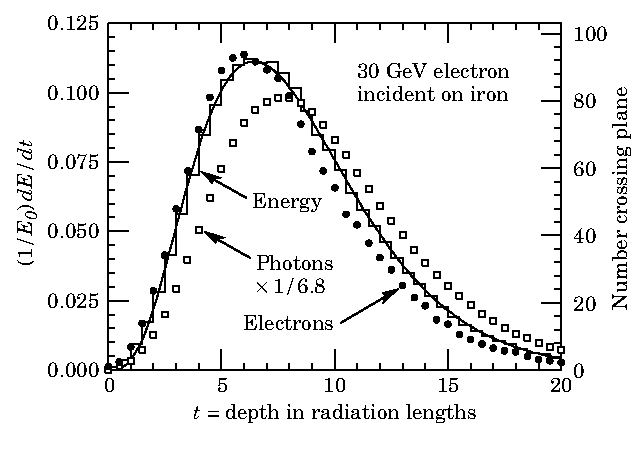
\includegraphics[scale=1.4,keepaspectratio=true]{./ElecCascadeInIron.pdf}
 % ElecCascadeInIron.pdf: 308x219 pixel, 72dpi, 10.87x7.73 cm, bb=0 0 308 219
 \caption{A simulation of a 30~GeV electron inducing a cascade in iron. The histogram shows the fractional energy deposition per radiation length, and the curve uses a gamma function fit to the distribution. Circles indicate the number of electrons with total energy greater than 15~MeV crossing planes at radiation length $X_{0}/2$ intervals and the squares indicate the number of photons with $E\geq 1.5$~MeV crossing planes (scaled down to have the same area as the electron distribution) \cite{pap:PDG}.}
%got this from PDG book: Fig.27.18
 \label{fig:ElecCascadeInIron}
\end{figure}


\begin{figure}[p]
 \centering
 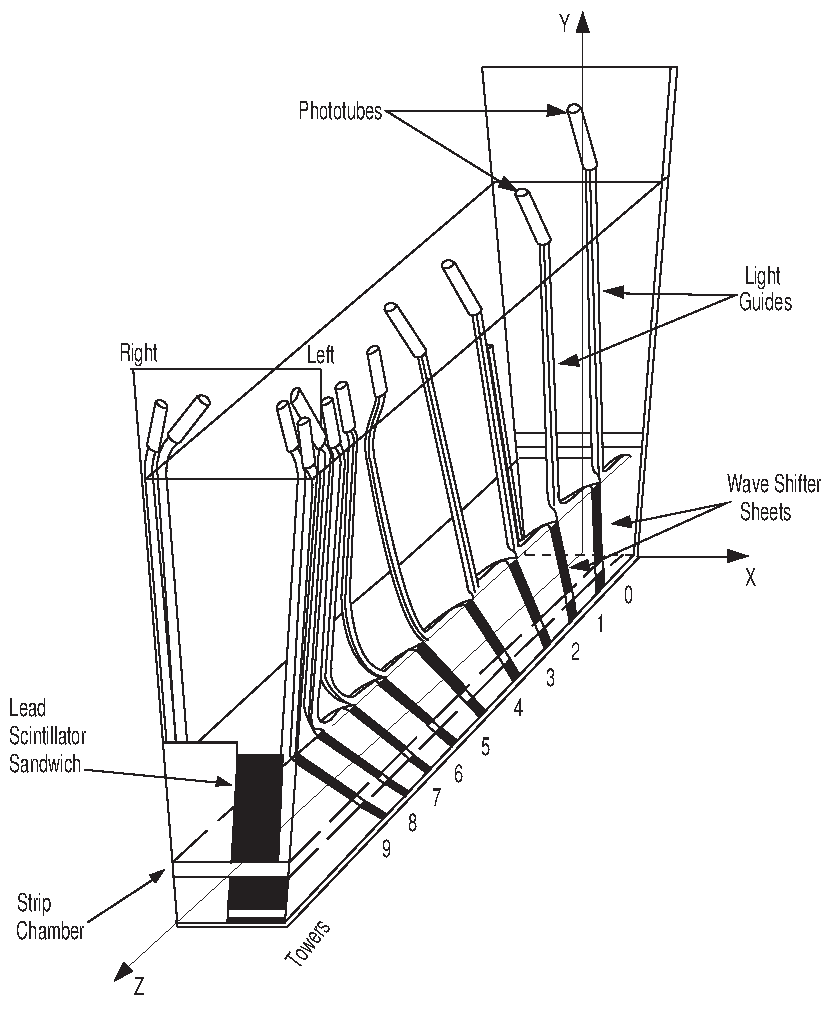
\includegraphics[scale=0.6,keepaspectratio=true]{./cdf_cem_wedge.pdf}
 % cdf_cem_wedge.pdf: 396x486 pixel, 72dpi, 13.97x17.15 cm, bb=0 0 396 486
 \caption{Schematic drawing of a single central calorimeter wedge.}
 \label{fig:CEMwedge}
\end{figure}


\begin{figure}[p]
 \centering
 \includegraphics[scale=0.5,keepaspectratio=true]{./plugCalSchem.pdf}
 % plugCalSchem.pdf: 689x567 pixel, 72dpi, 24.31x20.00 cm, bb=0 0 689 567
 \caption{Diagram of a plug calorimeter wedge.}
 \label{fig:PlugCalWedge}
\end{figure}

\vspace{-0.015\textheight}
The central electromagnetic calorimeter (CEM) (Fig.~\ref{fig:CEMwedge}) has an energy resolution of $\sigma(\et)/\et = 13.5\%/\sqrt{\et} \pm 2\%$ and the plug electromagnetic calorimeter (PEM) (Fig.~\ref{fig:PlugCalWedge}) has an energy resolution of $\sigma(\et)/\et = 16.0\%/\sqrt{\et} \pm 2\%$ for an electron. The central hadron calorimeter (CHA) and plug hadron calorimeter (PHA) energy resolution, as measured with pions, is $50\%\sqrt{E} \pm 3\%$ and $80\%\sqrt{E} \pm 5\%$, respectively \cite{pap:PlugCal}. A summary of the detector parameters is shown in Table~\ref{tab:Calo_parameters}.

\begin{table}[p]
\caption{Calorimeter parameters, thicknesses of active and passive materials, and energy resolutions.}
\label{tab:Calo_parameters}
\centering
\begin{tabular}{ccccc}
\hline
 & \BUbf{CEM} & \BUbf{PEM} & \BUbf{CHA} & \BUbf{PHA}\\
\hline
Thickness & 19~$X_{0}$, 1$\lambda$ & 21~$X_{0}$, 1$\lambda$ & 4.5$\lambda$ & 7$\lambda$ \\
Absorber & 0.6~$X_{0}$ & 0.8~$X_{0}$ & 25-50~mm & 50~mm \\
Scintillator & 5~mm & 4.5~mm & 10~mm & 6~mm \\
Resolution & $\frac{13.5\%}{\sqrt{E_{T}}} \pm 2\%$ & $\frac{16.0\%}{\sqrt{E_{T}}} \pm 2\%$ & $\frac{50\%}{\sqrt{E}} \pm 3\%$ & $\frac{80\%}{\sqrt{E}} \pm 5\%$\\
\hline
\end{tabular}
\end{table}

\subsection{Shower Maximum Detector}\label{sec:CES}
The Central Shower Maximum (CES)\glossary{name={CES}, description={Shower Maximum Detector}} detector is located at 7 radiation lengths inside the CEM (Fig.~\ref{fig:CEMwedge}) and provides measurements to determine the position and development of the transverse shower. A simulation of the shower development is shown in Fig.~\ref{fig:ElecCascadeInIron}. By measuring the charge deposition on the set of copper \newterm{strips} lying in the $z$-direction and \newterm{wires} lying orthogonal to strips (Fig.~\ref{fig:CESchamber}), it measures the azimuthal angle and $z$ position of the cluster. The position resolution for a 50~GeV electron is about 2~mm in each direction. The profile of the particle's shower measured by the CES and Plug Shower Maximum (PES) is used to discriminate photons from $\pi^{0}\to\gamma\gamma$ and from electrons. The detector parameters are shown in Table~\ref{tab:CESParamerters}.

\begin{figure}[hbtm]
 \centering
 \includegraphics[scale=0.89, keepaspectratio=true]{./ces_chamber.pdf}
 % ces_chamber.pdf: 492x246 pixel, 72dpi, 17.36x8.68 cm, bb=0 0 492 246
 \caption{CES wire and strip chamber.}
 \label{fig:CESchamber}
\end{figure}

\begin{table}[p]
\caption{Shower maximum detector parameters~\cite{pap:CDFCemCalorimeter}.}
\label{tab:CESParamerters}
\centering
\begin{tabular} {cc}
\hline
\BUbf{Parameter} & \BUbf{Value}\\
\hline
Radius from the beam line & 183.9 cm\\[1ex]
\textsc{Wire Channels (64)} & \\
Section 1 & 121.2 cm from the 90\degree edge\\
Wires & 32 $\times$ 1.45484 cm\\
Section 2 & 121.2--239.6 cm from the 90\degree edge\\
Wires & 32 $\times$ 1.45484 cm\\[1ex]
\textsc{Strip Channels (128)} & \\
Section 1 & 6.2--121.2 cm from the 90\degree edge\\
Strips & 69 $\times$ 1.67 cm\\
Section 2 & 121.2--239.6 cm from the 90\degree edge\\
Strips & 59 $\times$ 2.01 cm\\[2ex]
\multirow{3}{*}{\textsc{Total Thickness}} & 0.75 in.\\
& 0.069 radiation lengths\\
& 0.022 absorption lengths\\[2ex]
\textsc{Gas} 	& 95\%/5\% Ar/CO$_{2}$\\
\hline
\end{tabular}
\end{table}

\subsection{Muon Systems}\label{muon_system}
Often the energetic muons produced in collisions escape the CDF detector due to their high penetration power, leaving very little or no energy in the calorimeter. They do not generate a shower when they pass through the detector. The CDF muon detectors are stacked gaseous drift chambers. They form the outermost layer of subdetectors. They are designed to identify the ionization energy signature, and hits in chambers are combined to identify a track that indicates the presence of a muon in the event.

\subsection{Calorimeter Timing System}\label{EMTiming}
The timing readout for the electromagnetic calorimeters was installed as part of an upgrade for Run II. The system, known as \newterm{EM Timing}, has a resolution of less than a nanosecond and covers the central ($|\eta| < 1.1$) and plug ($1.1 < |\eta| < 2.1$) portions of the calorimeter \cite{pap:EMtiming}. A schematic diagram of the electronics of the system is shown in Fig.~\ref{fig:EMtimingSchematic}. The design of the EM Timing system is optimized for high-energy photons. It records the time of arrival of the particles that deposit large amounts of energy in the electromagnetic calorimeter. With this information it is possible to verify that all photons (or other energy) are from the primary collision, and also to reject or estimate the rate of cosmic-ray and beam-related backgrounds (see Section \ref{noncollision_backgrounds}). An overview of the EM Timing system parameters is listed in Table~\ref{tab:EMTimingPerformance}.

\begin{figure}[htb!]
 \centering
 \includegraphics[scale=0.5,keepaspectratio=true]{./EMtimingSchematic.png}
 % EMtimingSchematic.png: 785x574 pixel, 96dpi, 20.77x15.19 cm, bb=0 0 589 430
 \caption{A schematic diagram of the EM Timing system hardware on the CDF detector.}
 \label{fig:EMtimingSchematic}
\end{figure}

\begin{table}
\caption{Overview of the EM Timing system hardware and performance.}
\label{tab:EMTimingPerformance}
\centering
\begin{tabular}{lcc}
\hline
& \BUbf{CEM} & \BUbf{PEM}\\
\hline
Coverage & $|\eta|<1.1$ & $1.1<|\eta|<2.1$\\
Physical tower segmentation & $\Delta\phi=15\degree$, & $\Delta\phi=7.5\degree$,\\
& $\Delta \eta \approx 0.1 $ & $\Delta \eta \approx 0.1$\\[1ex]
Energy threshold & $3.8\pm0.3$~GeV & $1.9\pm0.1$~GeV\\
Timing resolution & $600\pm10$~ps & $610\pm10$~ps\\
\hline
\end{tabular}
\end{table}


\subsection{Extremely Fast Tracker (XFT)}
The eXtremely Fast Tracker (XFT) \cite{pap:XFT} is a vital part of the CDF trigger system. It is a trigger track processor that identifies charged tracks in the COT. This track information is made available to both Level 1 and Level 2 trigger decisions. The XFT is fully pipelined and provides track information for every event. The tracks are not fitted, but compared to predetermined patterns (or \newterm{roads}) derived using Monte Carlo methods. It is designed to measure tracks with momenta as low as \ptg{1.5}, to have high momentum and position resolution, and to minimize the fraction of tracks that are not associated with a real charged particle (\newterm{fake tracks}).

The XFT algorithm uses the hit information from the 4 axial superlayers of the COT. A charged track passing through an axial layer will generate a characteristic hit pattern in a 12-wire COT cell and will have a characteristic timing. The hit information in a superlayer is used by the Finders to search for track segments in the axial layers. Then the Linker will search and match track segments in the 4 superlayers to a track originated from the primary collision point. The Linker is able to search for tracks in 4/4 as well as 3/4 matches among the segments in the 4 layers.

As seen in Fig.~\ref{fig:XFTStructure}, the COT wire signals (pulses) are digitized by the Time-to-Digital Converters (TDC). The TDCs output the arrival time of the pulses (or time indices). The XTC mezzanine cards, mounted on the TDCs, use these time indices to categorize the hits on the COT wires into \newterm{prompt} ($<44$~ns) or \newterm{delayed} ($>44$~ns). The XTC sends the information to the Finder for processing.

\begin{figure}[htbm!]
 \centering
 \includegraphics[scale=0.14,keepaspectratio=true]{./XFTStructure.png}
 % XFTStructure.png: 774x470 pixel, 96dpi, 20.48x12.43 cm, bb=0 0 580 352
 \caption{Design of the XFT system. The upgrade added the stereo superlayer information to the existing axial system to enhance the track purity. The new fiber optic data path via XTC2$\to$Stereo Finder is merged with the axial system by the Stereo Linker Association Module, which associates the axial track segments with stereo track segments. The track information is then passed onto Level 2 decision-making and to the vertex detector.}
 \label{fig:XFTStructure}
\end{figure}
\vspace{-0.01\textheight}

The XFT was upgraded in summer of 2006 to handle the increased instantaneous luminosity. This was necessary as the higher luminosity increases the COT occupancy and produces many more fake tracks, which leads to a higher trigger rate. To handle this, the existing axial system was kept intact and the Stereo Finder system was added. The hit information from the 4 stereo superlayers is used by the Stereo Finder system to find track segments and confirm the association of those segments with the axial track segments. This also allows the measurement of the track's $z$ direction to match with the calorimeter or muon chambers.

The boxes colored in orange and blue in Fig.~\ref{fig:XFTStructure} indicate the new components. The new XTCs (called XTC-2) are able to classify hits into 6 programmable time windows. The Stereo Finder uses this information to identify track segments in the stereo layers. The Stereo Linker Association Module (SLAM) associates stereo track segments with the axial tracks. The performance of the XFT system is summarized in Table~\ref{tab:XFTperformance}.

\begin{table}
\caption{Performance of the XFT system as measured by data.}
\label{tab:XFTperformance}
\centering
\begin{tabular}{lc}
\hline
\BUbf{Parameter} & \BUbf{Value}\\
\hline
Efficiency & 96\% \\
Percentage Fakes & 3\% \\
Momentum Threshold & 1.5~\epUnits \\
Momentum Resolution & 1.7\%/\epUnits \\
Angular Resolution & 5.5~mR\\
\hline
\end{tabular}

\end{table}

The XTC and Finder electronics are designed with Field Programmable Gate Arrays (FPGA), which allow one to program custom logic designs into the electronics. The author performed preliminary testing of the XTC-2 cards and Finder boards and has implemented software packages to reprogram the XTC-2s and Finders. The conventional Finder FPGA reprogramming was sequential. Given that the Axial Finder boards require the loading of 4 logic designs, and each design requires about 20~s to download, reprogramming 48 of them took a considerable amount of time.

\begin{sidewaysfigure}[p]
 \includegraphics[scale=0.5,keepaspectratio=true]{./FlashRAMprogram.png}
 % FlashRAMprogram.png: 1215x737 pixel, 72dpi, 42.86x26.00 cm, bb=0 0 1215 737
 \caption{Graphical interface of the Finder Flash RAM program.}
 \label{fig:FlashRAMprogramming}
\end{sidewaysfigure}

This shortcoming was overcome by introducing a novel parallel programming technique known as \newterm{multithreading}. In general, multithreading forks a computer program into two or more concurrently running tasks or processes with the aid of techniques like time-division multiplexing to share the CPU time effectively among tasks. With this technique, all 48 of the Finder boards can be loaded with a specific design at once. The program is capable of job queuing to further reduce the downtime and speed up the Finder reprogramming. The interface of the program is shown in Fig.~\ref{fig:FlashRAMprogramming}. In addition, it can program a single Finder board with a specific software design and it can check the download status and the loaded software version on the boards.

Furthermore, the author developed software to reprogram XTC-2 cards from the unix command line. This is especially useful when working remotely with slower network connections. Also, the old \newterm{cratemap} program was updated to suit the upgrade system. The cratemap program scans crates holding the TDCs, Finders, etc. and provides information about the boards loaded into crates and their software versions and other information for diagnostics.

\subsection{Track Extrapolation Module (XTRP)}
The Track Extrapolation Module, XTRP for short, is part of the L1 trigger system driven by the information from the XFT. The XTRP distributes information derived from the tracks to make Level 1 and Level 2 trigger decisions. It performs three main tasks as shown it Fig.~\ref{fig:XTRPdataflow}. It extrapolates tracks to the central muon system and sends the information to the Level 1 MUON trigger. Similarly, information about tracks extrapolated to the central calorimeter is sent to L1 CAL trigger. Also, it selects tracks above a given \pt threshold and uses \pt and $\phi$ information to define the Level 1 TRACK trigger. Finally, the track information is passed on to Level 2 processing and the SVX upon a Level 1 accept.

\begin{figure}[htb!]
 \centering
 \includegraphics[scale=0.6]{./XTRP_dataflow.png}
 % XTRP_dataflow.gif: 720x540 pixel, 72dpi, 25.40x19.05 cm, bb=0 0 720 540
 \caption{Dataflow of the XTRP system.}
 \label{fig:XTRPdataflow}
\end{figure}


\subsection{Triggering}\label{triggering}
The Tevatron physics objective is to produce and study rare events. With a beam crossing interval of 396~ns, about a million events are generated every second. With the total inelastic cross section of about 60~mb, extracting signals of interest in an efficient way is an enormous challenge. Also, system limitations allow the recording of only a relatively small number of events per second. The solution is a \newterm{trigger} which will flag an event that satisfies a certain set of predefined kinematic thresholds (\textit{e.g.} transverse track momentum, calorimeter energy) and objects (\textit{e.g.} electron, muon, jet). A trigger is designed with a specific physics motivation and implemented after an extensive study. A collection of such individual triggers form a \newterm{trigger table}. The CDF trigger rejection is about 25000.

An efficient trigger requires fast object reconstruction and matching of tracks with the objects. The trigger matches COT tracks with EM calorimeter showers, muon chamber stubs, and silicon detector data in making a decision to save an event for physics analysis.

The CDF has a three-tier trigger system that is fully pipelined and hence deadtimeless (See Figs.~\ref{fig:TriggerSystemDetParts} and ~\ref{fig:TriggerSystemSchematic}). It is capable of dynamically limiting the acceptance of certain high rate processes as the luminosity changes. The \newterm{Level~1} trigger system is entirely hardware based, optimized for a quick decision. It forms trigger primitives by reading out a subset of detector components (like the tracking systems and calorimeters) and makes the initial decision to process the event further. Level~1 makes its decision to further process the event based on the information from the XFT, calorimeter, and muon data as seen in Fig.~\ref{fig:TriggerSystemDetParts}.

\begin{figure}[p]
\begin{centering}
\includegraphics[scale=0.7]{CDFTriggerSystem_DetParts.pdf}
\caption{Block diagram of the CDF three-level trigger system. This shows the detector information available at each decision level.}%Some detector components readout time is significantly large and is not used in initial decision making.}
\label{fig:TriggerSystemDetParts}
\end{centering}
\end{figure}

\begin{figure}[p]
\begin{centering}
\includegraphics[scale=0.8]{CDFTriggerSystem_Scehmatic.pdf}
\caption{Dataflow of CDF \newterm{deadtimeless} trigger system. Optimized by fully pipelining the system to match the physics event rate to the data acquisition rate.}
\label{fig:TriggerSystemSchematic}
\end{centering}
\end{figure}


The \newterm{Level 2} trigger is a combination of hardware and software and the output rate is lower. It also has more information available to make a more accurate decision. \newterm{Level 3} is entirely software-based and makes its final decision by completely reconstructing the event. The final output rate to tape is about 100~Hz. Overall, the trigger system rejects 99.99\% of events produced.


%Acceptance is defined as the probability that the generated (Monte Carlo) particles pass transverse energy (\et) , detector $\eta$ and other geometric cuts such as the azimuthal separation between objects. The efficiency is probability to survive all other sources of event losses.The distinction is that the acceptance can be calculated by anyone with access to a MC generator such as PYTHIA. The efficiency requires a detailed simulation of the detector with additional corrections and cross checks from data samples.


\subsection{Run Number, Run Section, and Run Period}
Each continuous data collection period is identified by a integer called a \newterm{run number}. To prevent data loss during a \newterm{run}, data are subdivided into about 15~sec periods called \newterm{run sections}. The importance of this is, for example, if a certain detector component is recognized to be at fault during a run, but not necessarily throughout the whole run, by identifying the time the fault occurred, data collected until that point can be recovered. A run period is about 2--3 months worth of data-taking time and depends on many factors like the amount of data collected and the detector operation status.

\subsection{Good Run List}\label{sec:GoodRun}
For some analyses, not all the information from the whole detector is needed. Information from certain subdetector components may not be crucial and may be omitted. An analysis expert will make a list of run numbers that had the required detector components running while the data of interest was collected. This list of run numbers is called a \newterm{good run list}. For photon analyses, it is necessary for COT, CES/PES, and calorimeters to be marked good. This study uses the good run list labeled by \goodrunfile.




\chapter{Monte Carlo Event Simulation}\label{chp:MCSimulation}
\vspace{0.015\textheight}
This chapter gives an overview of the simulation of events from \ppbar collisions. First, a simplified view of a \ppbar collision is presented and concepts related to different aspects of \ppbar collisions are introduced. Next, a more formal introduction to a \ppbar collision is given. Then, the \pythiaText event generator is described together with the scheme used to model the evolution of partons to stable, observable particles. Finally, a brief description of the CDF detector simulation is provided.

\section{The Proton-Antiproton (\ppbar) Collision}
The colliding protons and antiprotons are in the relativistic regime and so are their constituents, the partons. As the two beams pass through one another (in a beam crossing), a parton within a proton from one beam will collide with a parton within an antiproton from the other beam, traveling in the opposite direction. Often, these collisions are inelastic and produce ``soft'' (low momentum) particles. An occasional elastic collision (a hard scatter) may produce new and heavy particles. %This is an overly simplified descriptions of a hard scattering event. Next few paragraphs will explains the intermediate steps in a purely pedagogical manner. The actual understanding of the details in a hard scatter process is limited.

Figure~\ref{fig:ppbar_collision} is an illustration of a typical 2-to-2 parton hard scattering process in a proton-antiproton collision. In a 2-to-2 process, two incoming partons interact and produce two outgoing partons. As the two incoming partons approach each other, they can exchange virtual particles and radiate real particles (for example, gluons and photons). This radiation is termed \newterm{initial state radiation} (ISR). Similarly, outgoing partons can radiate particles and this is termed \newterm{final state radiation} (FSR). The partons from the broken proton and antiproton that did not take part in the hard scatter are called \newterm{spectator partons} and are also referred to as \newterm{beam remnants}. These spectator partons may interact by exchanging gluons and radiating particles to form stable particles. However, these stable particles tend to be softer, which means they have smaller momenta on average. These interactions form the \newterm{underlying event}, which overlaps with the hard scatter process. The underlying event generates particles that are detected in the tracking system and calorimeters. Often, the energy deposited in the calorimeters from the underlying event is indistinguishable from the energy of particles produced in the primary hard scatter.

\begin{figure}[htbm]
 \centering
 \includegraphics[scale=0.4,keepaspectratio=true]{./ppbar_collision.png}
 % ppbar_collision.png: 1047x528 pixel, 96dpi, 27.70x13.97 cm, bb=0 0 785 396
 \caption{A simulation of a hard 2-to-2 parton scattering process in a \ppbar collision. The \newterm{hard scatter} component consists of the interaction between an incoming parton in the proton and an incoming parton in the antiproton. The interaction produces two outgoing partons (detected as \newterm{jets}), plus ISR and FSR. The \newterm{underlying event} originates from interactions between the remnants of the proton and antiproton.}
 \label{fig:ppbar_collision}
\end{figure}
\vspace{-0.01\textheight}
%Such a event contains particles that originate from the two outgoing partons plus ISR/FSR, and particles from the broken $p$ and $\bar{p}$ (beam remnants).

It is also possible for more than one pair of partons to interact in the same proton-antiproton collision. If two such scattering processes occur, it is \newterm{double-parton scattering}. In this case, it is likely that the second interaction will be quite soft compared to the hard scatter.

Because of the large number of protons and antiprotons circulating in bunches, it is very common to have multiple protons collide with antiprotons in a given bunch crossing. These are known as \newterm{multiple interactions} (MI), and in principle each collision could have a hard scatter. However, in practice, a hard scatter is rare, and multiple interactions usually result in the production of soft particles. Just like the underlying event, particles associated with multiple interactions are difficult to distinguish from the primary hard scatter.

\subsection{Formalism of Hadron Collisions and Perturbative QCD (pQCD)}
\label{sec:pQCD}

The heart of perturbative QCD (pQCD) is the fundamental assumption of asymptotic freedom of the strong coupling constant. Assuming that the strong coupling constant \alphas is small at high-energy (short-distance) interactions, one can approximate such processes by perturbation theory.

QCD provides the formalism to calculate cross sections in high-energy hadron interactions. The cross section for a $2\to2$ hard scattering process (see Fig. \ref{fig:HadHadScattering}) where, for example, a hadron $h$ is produced by $pp \to hX$, can be expressed as:
\begin{eqnarray}
 \frac{d\sigma^{pp\to hX}}{dP} = \sum_{f_{1},f_{2},f} \int dx_{1} dx_{2} dz f_{1}^{p}(x_{1},\mu^{2}_{F}) f_{2}^{p}(x_{2},\mu^{2}_{F}) \nonumber\\*[1.5ex]
 \times \frac{d\hat{\sigma}^{f_{1}f_{2}\to fX^{\prime}}}{dP}(x_{1}p_{1},x_{2}p_{2},p_{h},\mu_{R})\times D_{f}^{h}(z,\mu^{2}_{f})
\end{eqnarray}
where $P$ is any appropriate kinematic variable of the interaction. The quantities $p_{1}$ and $p_{2}$ are the momenta of the initial partons, and $f_{i}^{p}(x_{i},\mu)$ is the probability density function for a parton type $f_{i}$ in the proton to have a momentum fraction $x_{i}$ at a given factorization scale $\mu_{F}$. This is also known as a Parton Distribution Function (PDF). The parameter $\mu_{F}$ is an arbitrary parameter used to avoid singularities in the formulation. There are many different PDF parameterizations, for example CTEQ \cite{pap:CTEQPDF} and MRST \cite{pap:MRSTPDF}. In this analysis, all of the MC samples were generated using the CTEQ5L (leading-order) PDFs. Furthermore, the CTEQ5L PDFs have been compared to MRST PDFs as a way to measure the uncertainty in the CTEQ5L PDFs. Distributions of the PDFs at two different energy scales are shown in Fig.~\ref{fig:PDFsDistributions}.

\begin{figure}[htbm!]
 \centering
 \includegraphics[scale=0.4,keepaspectratio=true]{./hh_collision.pdf}
 % hh_collision.pdf: 711x382 pixel, 72dpi, 25.08x13.48 cm, bb=0 0 711 382
 \caption[Schematic of a $2\to2$ hadron interaction.]{Schematic of a $2\to2$ hadron interaction. The overall interaction is a combination of three parts: the PDFs of the interacting partons, the partonic cross section $\hat{\sigma}$, and the fragmentation of the outgoing partons.}
 \label{fig:HadHadScattering}
\end{figure}

\begin{figure}[p!]
 \centering
 \subfigure[CTEQ5L PDFs]{
 \includegraphics[scale=0.35,keepaspectratio=true]{./CTEQ5PDFs_Distributions.png}
}
\subfigure[CTEQ6M PDFs]{
\includegraphics[scale=0.3,keepaspectratio=true]{./PDFs_Distributions.png}
 % PDFs_Distributions.png: 1774x857 pixel, 96dpi, 46.93x22.67 cm, bb=0 0 1330 643
}
 \caption{Overview of parton distributions functions: (a) the CTEQ5L PDFs (leading-order) at $Q^{2}=500$~GeV$^{2}$ \cite{pap:CTEQ5LPDFs} and (b) the CTEQ6M PDFs (next-to-leading order) at $Q=2$ and $Q=100$~GeV \cite{pap:CTEQ6MPDFs}. Several MRST PDFs are overlaid for comparison.}
 \label{fig:PDFsDistributions}
\end{figure}

The quantity $\hat{\sigma}^{f_{1}f_{2}\to fX^{\prime}}$ is the parton cross section calculated at a given order in pQCD and at a renormalization scale $\mu_{R}$. This is the cross section for initial partons with $f_1$ and $f_2$ to produce a final-state parton $f$ and unobserved parton $X^{\prime}$. $D_{f}^{h}(z,\mu^{2}_{f})$ is the fragmentation function, which is the probability density for finding $h$ with fraction of momentum $z$ in the final-state parton $f$ at some fragmentation scale $\mu_f$.

The Factorization Theorem allows one to factorize this total cross section into three parts: the PDF, the parton cross section, and the fragmentation function. This allows the separation of high-energy perturbative processes from low-energy non-perturbative processes. The partonic cross section, $\hat{\sigma}$, can be evaluated perturbatively. But the PDFs ($f_{i}^{p}(x_{i},\mu)$) and fragmentation functions ($D_{f}^{h}(z,\mu^{2}_{f})$) cannot be evaluated perturbatively.

\section{\pythiaText Event Generator}
Event generators, which are based on theoretical calculations, are used to generate physics processes as observed in data. They are used to validate the SM and test for extensions to the SM. There are many different event generators with different capabilities and levels of accuracy. This analysis uses simulated events generated using the \pythiaText Monte Carlo event generator with Tune~A \cite{pap:PythiaManual}. It uses only the leading-order cross section to generate events. \pythiaText simulates the various aspects of a hadron collision: the hard scattering process, the underlying event, and multiple interactions. Then, the different components of the event are overlaid to create the final output.

\pythiaText uses LO matrix element calculations to generate a hard scatter between partons, and it is optimized for $2\to1$ and $2\to2$ scattering processes. Prompt photons are produced in $2\to2$ scattering processes as shown in Fig.~\ref{fig:SM_pj_Feynmans}. Those production process are described in Section~\ref{sec:gjetProdInSM}. Fragmentation, also known as hadronization, is the process whereby partons form colorless hadrons as a result of color confinement. \pythiaText uses \newterm{string} fragmentation. It assumes the quarks are held together by color lines of force that are similar to the electric lines of force between two electric charges as seen in Fig.~\ref{fig:StringFragmentation}. These strings are broken in such a way that color-singlet hadrons are formed out of the vacuum. Fig.~\ref{fig:StringFormation} shows how the strings are formed between partons in the formation of color singlets. This string breaking and formation quickly becomes nonperturbative and extremely hard to calculate. To overcome this difficulty, an object called a \newterm{jet} is defined. By defining a jet, one can ignore the interactions between individual particles (or the higher-order contributions) and avoid the non-perturbative regime altogether. The hadronized particles from a parton will be seen as a collimated spray of particles in the detector. A jet is comprised of charged and neutral particles that are both hadronic and leptonic.

\begin{figure}[htbm!]
 \centering
\subfigure[]{
 \includegraphics[scale=0.4,keepaspectratio=true]{./LundStringModel.pdf}
}
\subfigure[]{
 \includegraphics[scale=0.5,keepaspectratio=true]{./LundStringModel2.pdf}
}
\caption{(a) Electric lines of force between two charges. (b) Color lines of force between quarks are pulled together into a tube or string because of the self-interaction between the gluons.}
\label{fig:StringFragmentation}
\end{figure}

\begin{figure}[htbm!]
 \centering
\subfigure[]{
 \includegraphics[scale=0.23,keepaspectratio=true]{./StringFormationInQQsystem.png}
}\\
\subfigure[]{
 \includegraphics[scale=0.13,keepaspectratio=true]{./StringFormations.png}
}
\subfigure[]{
 \includegraphics[scale=0.17,keepaspectratio=true]{./StringFormations2.png}
}
 \caption{(a) Overview of hadron production in a $q\bar{q}$ system. (b) Formation of strings between partons. (c) As partons are pulled apart, the potential energy increases and eventually partons are created out of the vacuum to produce colorless hadrons.}
 \label{fig:StringFormation}
\end{figure}

Since \pythiaText cross sections and branching ratios are based on LO calculations they can differ significantly from the theoretical next-to-leading-order (NLO) calculations. As an ad hoc fix to this, LO \pythiaText cross sections are multiplied by a constant factor called a \newterm{$k$-factor}. The $k$-factor is defined by
\begin{equation}
 k=\frac{\sigma(\mbox{NLO})}{\sigma(\mbox{LO})}.
\end{equation}

The $k$-factors can vary depending on how the cross sections are calculated. Cross sections for all of the \pythiaText MC samples used in this analysis have been corrected with a factor of $k=1.4$.

Within \pythiaText, initial-state radiation is computed in backward evolution. Every step in the parton evolution is \pt-ordered and there is an artificial cutoff on the allowed radiation to avoid singularities. Once the parton evolution is complete and stable particles are formed, they are passed into the detector simulation.

%Once an event is generated, minimum bias events are overlaid to improve the modeling of the underlying event and multiple interactions. Minimum bias data are events with no bias from restricted trigger conditions. They include events from nonelastic and diffractive process too. \pythiaText includes only non-diffractive and double-diffractive events in the minimum bias modeling.

\section{Detector Simulation}\label{sec:cdfsim}
A simulation of the CDF detector (\cdfsimText) \cite{www:CDFSIM} is based on a software package called \geantText (GEometry ANd Tracking) \cite{www:GEANT}. \geantText takes into account all the material in the CDF detector as seen in Fig.~\ref{fig:CDFinGEANT}. Every aspect of the detector is carefully accounted for and implemented in the software. The generated particles are tracked by \geantText as they traverse the CDF detector, and secondary physical processes such as energy loss, multiple scattering, and inelastic interactions are simulated. After the first inelastic interaction in the calorimeter, the particles are passed to a program called \gflashText \cite{pap:GFLASH}, which simulates electromagnetic and hadronic particle showers. \gflashText, which uses parameterizations of the calorimeter response, generates particle shower shapes within the calorimeter. The calorimeter parameterization is derived from the response of single particles using test beam data and minimum bias data.

\begin{figure}[htb!]
 \centering
 \includegraphics[scale=0.4,keepaspectratio=true]{./CDFinGEANT.png}
 % CDFinGEANT.png: 1301x1021 pixel, 96dpi, 34.42x27.01 cm, bb=0 0 976 766
 \caption{CDF detector volume implemented in \geantText.}
 \label{fig:CDFinGEANT}
\end{figure}




\chapter{Object Reconstruction and Identification}\label{chp:ObjectReco}
\vspace{0.015\textheight}
In order to understand how particles are produced and how they interact, one needs to study the actual physics process occurring at the interaction point. To do this, the particles produced in a \ppbar interaction are used to infer the original physics process. The produced particles, as they traverse the detector, interact with it and generate electronic signals. Those electronic signals are used to recreate the particles' properties, such as their energies and momenta, as well as the location of the interaction point. From this information, the actual interaction can be completely reconstructed. The process of converting electronic signals into particles that can be used in physics analyses is called \newterm{event reconstruction}. In this chapter, the reconstruction and identification of photons, electrons, and jets are described in detail. This chapter also describes the energy corrections to the measured jets. Finally, definitions of several kinematic quantities measured in the analysis are given.

\section{Photon Identification}\label{sec:photon_identification}

In order to identify a photon, information from various subdetector components is combined using the following general procedure.  First, individual detector segments (towers, wires, or scintillator tiles) that have a signal above a predetermined minimum threshold are identified.  Then, the qualifying segments are grouped to form \newterm{clusters}. The formation of the clusters is tuned and optimized in each type of subdetector component based on its design. In most situations, iterative algorithms are used to identify and form these clusters. The final measurement of the photon is done based on this clustered energy.

\subsection{Calorimeter Energy Clustering}
Calorimeter towers containing energy deposited by photons produced in the hard scattering process are grouped to form energy clusters via a clustering algorithm. First, the whole detector is searched for towers with a transverse energy above a minimum threshold ($\sim$100~MeV), and these towers are considered in the clustering process. The towers are sorted by decreasing \et and seed towers with $E_{T}>3$~GeV are selected. Finally, towers within a rectangular grid ($3\times 3$) around the seed towers are considered for inclusion in the EM clusters. The grid size is reduced to $2\times 2$ in the plug calorimeter photon reconstruction to reduce effect of jets. Energy in a cone of radius $\Delta R=\sqrt{\Delta\eta^{2}+\Delta\phi^{2}}=0.4$ (see Fig.~\ref{fig:PhotonIsoCone}), centered on the seed tower, generally should include almost all of the energy of a single photon or electron. Initial EM clustering is always done assuming the primary interaction is located at $x=y=z=0$ \cite{cdfnote:5456}. (This is also true for clustering jets.)

\begin{figure}[htb!]
 \centering
 \includegraphics[scale=0.35,keepaspectratio=true]{./PhotonIsolationDemo.png}
 \caption{A geometric cone is used to reconstruct a photon in the detector. Reconstruction requires the photon to be isolated by limiting the extra energy surrounding it.}
 \label{fig:PhotonIsoCone}
\end{figure}

The total energy ($E$) of the cluster includes the sum of the energies of the EM ($E_{EM}$) and HAD ($E_{HAD}$) calorimeters. The coordinates of the EM cluster are initially derived by an energy-weighted method as described below.

First, $\eta_{EM}$ and $\phi_{EM}$ are calculated using the EM towers in the cluster and $\eta_{HAD}$ and $\phi_{HAD}$ using the HAD towers in the cluster.
\begin{eqnarray}
 \eta_{EM} &=& \frac{\sum_{i}E^{i}_{EM}\cdot\eta^{i}}{\sum_{i}E^{i}_{EM}}\\
 \phi_{EM} &=& \frac{\sum_{i}E^{i}_{EM}\cdot\phi^{i}}{\sum_{i}E^{i}_{EM}}\\
 \eta_{HAD} &=& \frac{\sum_{i}E^{i}_{HAD}\cdot\eta^{i}}{\sum_{i}E^{i}_{HAD}}\\
 \phi_{HAD} &=& \frac{\sum_{i}E^{i}_{HAD}\cdot\phi^{i}}{\sum_{i}E^{i}_{HAD}}
\end{eqnarray}
Then the actual coordinates are calculated using
\begin{eqnarray}
 \eta &=& \frac{E_{EM}\cdot\eta_{EM}+E_{HAD}\cdot\eta_{HAD}}{E}\\
 \phi &=& \frac{E_{EM}\cdot\phi_{EM}+E_{HAD}\cdot\phi_{HAD}}{E}
\end{eqnarray}
Finally, the energy of the (photon) cluster is corrected by measuring its position in the CES with respect to the primary vertex. Then, using the polar angle ($\theta$), the transverse energy of the photon cluster can be calculated using
\begin{equation}
 E_{T} = E\cdot\mathrm{sin}(\theta)
\end{equation}

\subsection{CES Energy Clustering}
There are two types of CES energy clustering algorithms; one is \newterm{track-based} and the other is \newterm{strip-based}.

The \newterm{strip-based} or \newterm{unbiased} CES clustering sorts the strips/wires by decreasing energy and seeds the cluster with the highest energy strip. Then, a strip/wire collection is formed by gathering $N$ strips around the seed, where $N$ is a tunable parameter. All the strips belonging to clusters are tagged and removed from the remaining collection of strips. Hence, a strip cannot belong to two clusters, unlike in the track-based clustering. This clustering method is specifically designed for photon identification.

The \newterm{track-based} algorithm, which is designed mostly for charged electromagnetic particles (i.e.~for electrons), finds the seed of the cluster by extrapolating a track to the CES radius. Then it records the $x$ and $z$ coordinates of the track in the CES local coordinate system. Finally, it forms a strip collection by finding the strip that is hit and adding $N$ number of strips around the seed strip where $N$ is a tunable parameter. The result is that all the tracks in an event passing some minimum quality selection requirements are associated with a CES cluster.

\subsection{Photon Selection Requirements}
A combination of kinematic and fiducial selection requirements are applied sequentially to the EM clusters to identify photon candidates. Offline calibration and calorimeter energy scale corrections are applied to the calorimeter energy cluster. The standard photon selection requirements include a minimum corrected transverse energy (\etcorr) greater than \etg{7}. The CES fiducial selection requirements make sure the cluster (shower) is contained within the instrumented regions of the detector. The CES shower position is determined by the \et-weighted centroid of the highest energy clusters of those strips and wires in the CES that correspond to the seed tower. The direction of the photon can be inferred by connecting the primary event vertex and the CES shower position. Being an electromagnetic object, photons are expected to lose all of their energy inside the EM calorimeter. The selection requirement, $E_{HAD}/E_{EM}$, the ratio of the total energy in the hadron calorimeter to the total energy in the EM calorimeter, is derived from this basic idea. This limits the number of jets identified as photons (or electrons). The presence of a track or tracks is used to distinguish photons from leptons and jets. At most one reconstructed track is allowed, and the \pt of that track should be small. This allows an increase in efficiency that otherwise would be lost due to a random low-\pt track from the underlying event. The isolation energy requirement further suppresses the lepton and jet backgrounds and is the most effective requirement for removing jets.
The variables used for photon identification are presented below together with the standard tight and loose photon selection requirements. Table~\ref{tab:tightAndLoosePhotonCuts} has a summary of the selection requirements. The photon candidate energy is corrected for the calorimeter energy response, the underlying event, and multiple interactions.

\begin{table}[p]
\caption{Standard Tight and Loose Photon selection requirements.}
\label{tab:tightAndLoosePhotonCuts}
\centering
\begin{tabular} {ccc}
\hline
\BUbf{Selection Variable} 	& \BUbf{Standard Requirement} & \BUbf{Loose Requirement}\\
\hline
detector ($\eta^{detector}$) 	& \etalessthan{1.1} & \etalessthan{1.1}\\
$\etcorr$ 	& \etg{30}	& \etg{30} \\[2ex]
CES X and Z & $ |X_{CES}| \leq 21 $ cm 	& $ |X_{CES}| \leq 21 $ cm\\
 fiducial & 9 cm $ \leq |Z_{CES}| \leq 230 $ cm 	& 9 $\leq|Z_{CES}|\leq230$ cm\\[2ex]
\multirow{2}{*}{$E_{HAD}/E_{EM}$} & $\leq 0.125$ & \multirow{2}{*}{$<$ 0.125}\\
& $|| \leq 0.055 + 0.00045 \times \ecorr$&\\[2ex]
\multirow{4}{*}{\isoetcorr in cone 0.4}
& $\leq 0.1 \times \etcorr$ & $\leq 0.15 \times \etcorr$ \\
 & if $\etcorr<20$~\etUnits & if $\etcorr<20$~\etUnits\\
 & $\leq 2.0 + 0.02 \times (\etcorr -20)$ & $\leq 3.0 + 0.02 \times (\etcorr -20)$ \\
 & if $\etcorr>20$\etUnits & if $\etcorr>20$\etUnits\\[2ex]
average CES $ \chi^2$	& \multirow{2}{*}{$\leq 20 $} & No selection\\
(Strips+Wires)/2 & & requirement \\[2ex]
N tracks in cluster& \multirow{2}{*}{$\leq1$} & \multirow{2}{*}{$\leq1$} \\
 (N3D)\\[2ex]
Track $\pt$ 	& $< 1+0.005 \times \etcorr$ 	& $<0.25 \times \etcorr$\\
Track Iso($0.4$) & $< 2.0 + 0.005 \times \etcorr $ & $<5.0$\\[2ex]
\multirow{4}{*}{}
$E_{T}$ of the 2\superscript{nd} CES cluster &if $\etcorr<18$~\etUnits & \multirow{4}{*}{No Requirement}\\
(both wire and & $\leq 0.14\times\etcorr$ & \\
strip) & if $\etcorr\geq18$~\etUnits & \\
 & $ \leq2.4+0.01\times\etcorr$ & \\
\hline
\end{tabular}
\end{table}
%%%%%%%%%%%%%%%% END TIGHT PHOTN ID CUTS %%%%%%%%%%%%
%%%%%%%%%%%%%% LOOSE PHOTON CUT %%%%%%%%%%%%%
%\begin{table}[hbm]
%\begin{center}
%\begin{tabular} {|c|c|}
%\hline
%\BUbf{Selection Variable} 		& \BUbf{Requirement} 	\\
%\hline
%detector 		 	& central 	\\
%\hline
%$\etcorr$ 	& $ >30 $ GeV \\
%\hline
%CES X and Z fiducial 		& $ |X_{CES}| \leq 21 $ cm \\
%				& $ 9 $ cm $ \leq |Z_{CES}| \leq 230 $ cm \\
%\hline
%Had/EM 		&	$ \leq 0.125$ \\
%\hline
%\isoetcorr in cone 0.4	& $\leq$ 0.15 $\times \etcorr$ if $\etcorr<$20 GeV\\
%					& $\leq$ 3.0 if \etcorr$>$20 GeV \\
%\hline
%Track $\pt$ 	& $< 0.25 \times \etcorr$ \\
%\hline
%Track Iso($0.4$) &	$< 5.0 $ \\
%\hline
%\end{tabular}
%\end{center}
%\caption{Loose Photon selection requirements.}
%\label{tab:loosephotoncuts}
%\end{table}
%%%%%%%%%%%%%% END LOOSE PHOTON CUTS %%%%%%%%
\vspace{-0.01\textheight}
\begin{singlespace}
\begin{itemize}
\item {\cutVar{Detector} Pseudorapidity ($\eta^{detector}$) --- This is the detector region where the object is found. The CDF detector is divided into three regions: central, plug, and forward. The central part lies within \etalessthan{1.1} and the plug region extends from \etaabsregion{1.1}{3.5}. The forward region extends from \etaabsregion{3.5}{5.9} (see Fig.~\ref{fig:TrackingCoverage}). The central part of the detector is better instrumented and well understood compared to the other two regions.
}

\item{$E_{T}= E \times \mathrm{sin}(\theta)$ where $E$ is the electromagnetic energy of the cluster and $\theta$ is the polar angle. This is the transverse component of energy deposited by a photon in the calorimeter. Standard selection rules require $E_{T}>7$~GeV to qualify as a photon candidate. (As photons are massless, $\et=\pt$.)
}

\item{CES Fiducial ($X_{CES}$, $Z_{CES}$) --- The CES requirements are defined by the active region of the detector. Requiring an energy deposition in an area covered by both strips and wires ensures that the energy cluster is well contained within the instrumented regions of the detector. The fiducial region is defined by the CES local coordinates $|x|<21$ cm and 9~cm~$<|z|<$~230~cm. The CES wire (strip) clusters are formed from an 11-wire (strip) window around the highest-\et seed wire (strip). The highest-\et wire (strip) must be within 25~cm in $z$ of the EM centroid.
}

\item{Average CES $\chi^2$ --- The $\chi^2$ value is a measure of the shape of the lateral shower profile created by a particle. This is obtained by comparing the observed lateral shower shape in the CES strips and wires with that measured by a test beam for a single photon. The average of the $\chi^{2}$ values of strips and wires should be $<$20.
}

\item{$E_{HAD}/E_{EM}$ --- This is the ratio of the total energy of the energy cluster in the hadron calorimeter to the energy in the electromagnetic calorimeter. Electromagnetic objects like electrons, positrons, and photons deposit more energy in the EM calorimeter while hadrons deposit more energy in the HAD calorimeter.
}

\item{Isolation Energy (\isoetcorr) is defined as
\begin{equation}
\isoetcorr = E_{T}^{0.4} - E_{T}^{cluster}
\end{equation}
\noindent where $ E_{T}^{0.4} $ is the energy in the cone of radius \mbox{$ \Delta R = \sqrt{\Delta \eta^2 + \Delta \phi^2 } = 0.4$} around the cluster excluding the photon cluster, and $ E_{T}^{cluster}$ is the energy in the photon cluster. This is a measure of the energy surrounding the object. A well-isolated photon occupies one calorimeter tower and there is not much energy outside of the photon cluster. This will reduce the possibility of misidentification when there are many objects in close proximity.

A \newterm{leakage} of energy may occur when the photon energy is not fully contained in the cluster and some energy is smeared into the neighboring $\phi$ wedge(s). Therefore, the isolation energy is corrected for leakage. Also, it is corrected for multiple interactions. Multiple interactions in the same bunch crossing tend to add extra energy to the cluster that needs to be subtracted.
}

\item{\cutVar{N3D} Tracks and Track \pt\ --- A track pointing to the cluster is the strongest discriminator between a photon and an electron. If there is a clearly identified track pointing to the calorimeter energy cluster, it is most likely an electron. N3D is the number of tracks that hit the calorimeter cluster within 5~cm of the seed tower. The photon selection allows only one track, and its \pt must be smaller than the \pt shown in the Table~\ref{tab:pecuts}.
%(?? why do we even allow 1 track, why not use =0? Is this because then we can't model the fake leptons/jets correctly? especially if we plan to use the sideband to model the fake jets in the tight photon sample.)
% yes, if i want a pure photon sample better to use ==0. but there are two factors to consider.
%this (==1) is to increase acceptance and to use sideband to model fake in tight sample correctly. we may loose photons due to soft random tracks.
}

\item{Track Isolation --- Within the clustering cone of 0.4, there cannot be many tracks pointing to the photon cluster. If there are many tracks, the object might not be a photon, but a jet. This selection requirement constrains the sum of the transverse momenta of all the tracks within $5$~cm of the vertex and $\Delta R \leq$~0.4 compared to the direction of the cluster.
}

\item{Second CES Cluster --- If a pair of photons is produced from light meson decay (\textit{e.g.} \pizero$\to\gamma\gamma$), the calorimeter is unable to resolve them. The CES detector, however, may have information about an additional cluster indicating the second photon. Hence, by measuring the energy of a second CES cluster, one can reduce the misidentification of photons from meson decay. This requirement is most effective for energies $<$35~GeV; for larger energies, the CES is unable resolve the two photons. A photon candidate should not have a second CES cluster.
}

\end{itemize}
\end{singlespace}


\section{Electron Identification}
Electrons in the photon + jets events are identified for two reasons. The first reason is for crosschecks and testing. The second reason is to improve the accuracy of the \met measurement.

The identification of electrons follows the same general procedure as described at the beginning of the photon identification in Section~\ref{sec:photon_identification}. In addition, a COT track with \ptg{1} in association with the calorimeter energy cluster is required. A special set of selection requirements known as \newterm{photon-like electron} selection requirements are used to identify electrons (see Table~\ref{tab:pecuts}). These selection requirements are suitable for photon analyses as they exploit the fact that the most probable scenario for an electron to be misidentified as a photon is failure to reconstruct the associated track.

%%%%%%%%%%%%%%% PHOTON-LIKE ELECTRON ID CUTS %%%%%%%%
\begin{table}[hbmt!]
\caption{Photon-like electron selection requirements. The photon-like electron selection requirements are very similar to the photon selection requirements except that one extra high-\pt track is allowed. This is due to the fact that an electron candidate can fake a photon if the associated track is not reconstructed. %Hence, assuming the primary track is not constructed the track \pt and track isolation selection requirements are applied to the subleading track. Leading track's \pt is subtracted prior to applying the track isolation cut.}
}\label{tab:pecuts}
\centering
\begin{tabular} {cc}
\hline
\BUbf{Selection Variable} & \BUbf{Requirement} \\
\hline
detector ($\eta^{detector}$) & \etalessthan{}{1.1} \\
\etcorr & \etg{7} \\[2ex]
\multirow{2}{*}{CES fiducial} & $ |X_{CES}| \leq 21 $ cm \\
		& $ 9 $ cm $ \leq |Z_{CES}| \leq 230 $ cm \\[2ex]
average CES $ \chi^2 $	& $ \leq 20 $ \\
$E_{HAD}/E_{EM}$ & $ \leq 0.055 + 0.00045 \times E$ \\[2ex]
\multirow{2}{*}{\isoetcorr in cone 0.4}	& $ \leq 0.1 \times \et $ if $ \et < 20 $~\etUnits \\
 & $ \leq 2.0 + 0.02 \times (\et -20) $ if $ \et \geq 20 $~\etUnits \\[2ex]
N3D tracks in cluster	& $= 1,2 $ \\[2ex]
\multirow{2}{*}{\eoverp of 1st track} & $0.8 \leq \eoverp \leq 1.2 $ if $ \pt < 50 $~\epUnits \\
 & no requirement if $ \pt \geq 50 $~\epUnits \\[2ex]
2\textsuperscript{nd} track $\pt$ if N3D = 2 & $ \leq 1.0 + 0.005 \times \et $ \\
TrkIso($0.4$) - $\pt$(1st track) & $ \leq 2.0 + 0.005 \times \et $ \\[2ex]
\et of 2nd CES	& $ \leq 0.14 \times \et $ if $ \et < 18 $~\etUnits \\
cluster (wire and strip) & $ \leq 2.4 + 0.01 \times \et $ if $ \et \geq 18 $~\etUnits \\[2ex]
$|\Delta z| = z_{vtx} \-- z_{trk}$ & $\leq 3$ cm	\\
\hline
\end{tabular}
\end{table}


The downside to the photon-like electron selection requirements is that they are less efficient than the standard electron selection requirements. In order to improve the \met measurement, all possible EM objects need to be identified to avoid overcorrecting them by applying jet energy corrections. For this, the standard loose electron selection requirements are used. The standard loose central and plug selection requirements are listed in Table~\ref{tab:StdLooseCentalEleID} and Table~\ref{tab:StdLoosePlugEleID}. Most of these variables have the same definition as the photon selection requirements. The remaining electron identification variables are defined below.

%\cutVar{E} : Plug electron energy in GeV. The energy measured by $2\times2$ clustering algorithm.
\vspace{-0.01\textheight}
\begin{singlespace}
\begin{itemize}
\item {$\Delta z$ --- This is the closest-approach separation between the associated track of the electron candidate and the primary vertex of the event. By limiting the separation, one can be certain of the origin of the track and its association to the electron candidate. This reduces the electrons from conversions in which $\gamma\to ee$.}

\item{\cutVar{PES 2D $\eta$} --- The detector $\eta$ of the electron shower measured by the plug EM shower maximum detector (PES).}

\item{\cutVar{PEM $3\times 3~\chi^{2}$} --- This is a $\chi^{2}$ comparison of the energy distribution of the electron cluster in the $3\times3$ cluster around the seed tower to that of test beam data.}

\item{\cutVar{PES $5\times9$ U/V} --- The two layers (named U and V) of the PES detector provide a two-dimensional position measurement. A $5\times9$ ratio is used to describe the shape of the energy cluster. The ratio is measured as the energy deposited in a 5-wire window to that of a 9-wire window (the 5 wires plus two additional wires on either side).}

\item{$\Delta R$ --- This is the distance between the 2D position measured by the PES detector to that measured by the PEM calorimeter, defined as: $\Delta R = \sqrt{(x_\mathrm{pes}-x_\mathrm{pem})^{2}+(y_\mathrm{pes}-y_\mathrm{pem})^{2}}$.}
\end{itemize}
\end{singlespace}


% STD CEN ELECTRON ID CUTS
\begin{table}[hbmt!]
\caption{Standard loose central electron selection requirements.}
\label{tab:StdLooseCentalEleID}
\centering
\begin{tabular}{cc}
\hline
\BUbf{Selection Variable} & \BUbf{Requirement}\\
\hline
detector ($\eta^{detector}$) & \etalessthan{1.1}\\
\etcorr & \etg{7}\\[2ex]
\textsc{COT track} &\\
Axial SLs & $\geq3$ with $\geq8$ hits per SL\\
Stereo SLs & $\geq2$ with $\geq8$ hits per SL\\
Beam constrained $z_{0}$ & $\leq60$~cm\\
Track \pt & $\geq3.5$~\epUnits\\[2ex]
$E_{HAD}/E_{EM}$ & $\leq 0.055+0.00045\times E$\\
Iso(R=0.4) & $\leq 0.1$\\
CES fiducial & $=1$\\
Lshr & $\leq 0.4$\\
\hline
\end{tabular}
\end{table}


%%% STD LOOSE PLUG ELECTRON ID CUTS
\begin{table}[hbmt!]
\caption{Standard loose plug electron selection requirements.}
\label{tab:StdLoosePlugEleID}
\centering
\begin{tabular}{cc}
\hline
\BUbf{Selection Variable} & \BUbf{Requirement}\\
\hline
detector ($\eta^{detector}$) & $1.1<|\eta|<3.6$\\
\et & \etg{7} \\
PES 2D $\eta$ & $1.5<|\eta|<3.0$\\
$E_{HAD}/E_{EM}$ & $\leq 0.05$\\
PEM $3\times3~\chi^{2}$ & $\leq 10.0$\\
Iso~($R=0.4$) & $\leq 0.1$\\
CES fiducial & $=1$\\
\cutVar{PES $5\times9$ U/V} & $\leq 0.65$\\
$\Delta R$ & $\leq 3.0$\\
\hline
\end{tabular}
\end{table}


\section{Jet Identification}\label{sec:jet_identification}
In \ppbar collisions, an outgoing parton manifests itself as a cluster of collimated particles (both charged and neutral), which is referred to as a jet. A jet is also an abstraction from the theory of pQCD (see Section~\ref{sec:pQCD}). There are many definitions of a jet, as evident from Fig.~\ref{fig:jetdefinition}.

\begin{figure}[p]
\begin{centering}
\includegraphics[scale=0.14]{PartonJetPartcleJetAndCalJet.pdf}
\caption{Evolution of a jet. A parton jet is formed soon after the hard collision. A particle jet (or hadron-level jet) is formed after quarks and gluons hadronize into colorless particles. Finally, a calorimeter jet or (detector-level jet) is actually measured and observed in the detector using a clustering algorithm.}
\label{fig:jetdefinition}
\end{centering}
\end{figure}

\begin{figure}[p]
 \centering
 \includegraphics[scale=.5]{./JetClust_SingleCaloTower.png}
 % JetClust_SingleCaloTower.png: 903x613 pixel, 96dpi, 23.89x16.22 cm, bb=0 0 677 460
 \caption{Schematic of a single CDF calorimeter tower used in jet clustering.}
 \label{fig:jetClus_CaloTower}
\end{figure}


Identification of jets follows the same general concepts as described at the beginning of photon identification in Section~\ref{sec:photon_identification}. The energy of a jet is calculated from the energy deposited in the calorimeter towers (both EM and HAD) with the aid of clustering algorithms. There are many different clustering algorithms and each has its limitations. For this study, jets are clustered using a cone algorithm with a fixed cone size in which the center of the jet is defined as ($\eta^{jet}$, $\phi^{jet}$) and the size of the jet cone is $R = \sqrt{(\eta^{tower} - \eta^{jet})^{2} + (\phi^{tower} - \phi^{jet})^{2}} = 0.4$ (other options are 0.7 and 1.0). The jet clustering algorithm starts by identifying calorimeter towers with $E_{Ti}>1$~GeV to form seeds for jets, where $E_{Ti} = E_{i}\cdot\sin\theta _{i}$ is the transverse energy of a tower with respect to the $z$-position of the \ppbar interaction (see Fig.~\ref{fig:jetClus_CaloTower}), and the energy $E_{i}$ is the sum of the energies measured in the electromagnetic and hadronic compartments of that tower. The seed towers are sorted in order of decreasing $E_{Ti}$. Then, for each seed tower, towers within a radius $R$ of the seed tower's position are used to build clusters. The initial cluster transverse energy and the location of the cluster are calculated using the following definitions where $N_{tow}$ is the number of towers with $E_{T}>100$~MeV inside the radius $R$.
\begin{eqnarray}
 E^{jet}_{T} &=& \sum_{i=0}^{N_{tow}} E_{Ti}\\
 \phi^{jet} &=& \sum_{i=0}^{N_{tow}} \frac{E_{Ti}\phi_i}{E^{jet}_{T}}\\
 \eta^{jet} &=& \sum_{i=0}^{N_{tow}} \frac{E_{Ti}\eta_i}{E^{jet}_{T}}
\end{eqnarray}

For each cluster, this weighted average of the transverse energy in the cluster is used to identify the centroid of the cluster. Neighboring towers inside the cone with energies above the threshold are added and subtracted until a stable centroid is reached. Overlapping jets are merged if they overlap by more than the cutoff ($\sim$75\%). If the overlap is smaller, each tower in the overlap region is assigned to the nearest jets. The final jet energy, also known as \newterm{raw jet energy}, and momentum coordinates are computed from the final list of towers as described below.

\begin{eqnarray}
 E^{jet} &=& \sum_{i=0}^{N_{tow}} E_{i}\\
 p_{x}^{jet} &=& \sum_{i=0}^{N_{tow}} E_{i} \cdot \mathrm{sin}(\theta_{i}) \cdot \mathrm{cos}(\phi_{i})\\
 p_{y}^{jet} &=& \sum_{i=0}^{N_{tow}} E_{i} \cdot \mathrm{sin}(\theta_{i}) \cdot \mathrm{sin}(\phi_{i})
\end{eqnarray}

\begin{eqnarray}
p_{z}^{jet} &=& \sum_{i=0}^{N_{tow}} E_{i} \cdot \mathrm{cos}(\theta_{i})\\
p^{jet}_{T} &=& \sqrt{(p_{x}^{jet})^{2}+(p_{y}^{jet})^{2}}\\
\phi^{jet} &=& \mathrm{tan} (\frac{p_{y}^{jet}}{p_{x}^{jet}})\\
\mathrm{sin}(\theta^{jet}) &=& \frac{p^{jet}_{T}}{\sqrt{(p_{x}^{jet})^{2}+(p_{y}^{jet})^{2}+(p_{z}^{jet})^{2}}}\\
E_{T}^{jet} &=& E^{jet}\cdot\mathrm{sin}(\theta^{jet})
\end{eqnarray}


\section{Jet Energy Corrections}
The energies of clustered jets are corrected for detector effects, calorimeter response, and for physics-related effects. The sequence of corrections is described in the following section and described in detail elsewhere \cite{pap:JetCorrections}. % I have taken the text in the middle verbatim from the the citation, from section jet clustering.

\vspace{-0.01\textheight}
\begin{singlespace}
\begin{enumerate}
\item{\BUbf{$\eta$-dependent Corrections} --- Also known as the \newterm{relative corrections}, the $\eta$-dependent corrections are applied to raw jet energies to make the calorimeter response to jet energies uniform in $\eta$. These corrections are derived by measuring the transverse energy balance in dijet events. One jet is required to be in the central region of the detector (\etaregion{0.2}{0.6}) and the other is used as a probe. This is because the central calorimeter has a better resolution and is better understood. Figure~\ref{fig:JetCorrections_EtaDependence} shows the scale of this correction for different detector regions. Different corrections for data and simulated data samples are derived.}

\item{\BUbf{Corrections for Multiple \ppbar Interactions} --- At higher luminosity, more than one \ppbar interaction in a beam crossing can occur (see Chapter~\ref{chp:MCSimulation}). This may add extra energy to the clustering cone that needs to be removed. In such events, there will be more than one primary vertex. The corrections are derived using minimum bias data\footnote{These events are collected using a minimum bias trigger which requires hits in the east and west CLC detectors and no other requirements.} by measuring the transverse energy deposited in a random cone and parameterizing it as a function of the number of vertices in the event (see Fig.~\ref{fig:JetCorrections_MI}).}

\item{\BUbf{Absolute Corrections} --- After jet energies are corrected for $\eta$-dependence, they are further corrected for any non-linearity and energy loss in the uninstrumented regions of the central calorimeter. The absolute jet energy scale of the central calorimeter is determined by \pythiaText dijet \MC events. The observed calorimeter cluster energy (jet) is compared to the stable hadron-level jet which is identified using the same clustering algorithm. The scale of this correction is shown in Fig.~\ref{fig:JetCorrections_Absolute}.}

\item{\BUbf{Underlying Event Corrections} --- The underlying event (UE) is defined as the energy associated with the spectator partons in a hard collision event (see Chapter~\ref{chp:MCSimulation}). This extra energy needs to be subtracted from the jet energy in order to compare with the theoretical predictions involving only the hard collision. This correction is derived in a similar way to the corrections for multiple \ppbar interactions, using minimum bias data, but using events with only one primary vertex. The scale of these corrections for different clustering cone sizes is shown in Table~\ref{tab:JetCorrections_UE}.}

% \item{{\bf Out-of-cone Corrections} --- It is possible for a parton to radiate particles whose energy falls outside of the clustering cone. This out-of-cone energy needs to be added back to the particle jet. This corrects the particle jet energy for leakage of radiation outside the clustering cone used for jet definition and takes it back to \newterm{parent parton energy} (parton-level jet), which can be compared to theoretical predictions. The correction is derived using dijet \pythiaText \MC events. Hadron-level jets are matched to partons by requiring $\Delta R<0.1$ and is parameterized as a function of the hadron level jet energy (see Fig.~\ref{fig:JetCorrections_OOC}).}
\end{enumerate}
\end{singlespace}

\begin{figure}[p]
 \centering
 \includegraphics[scale=0.35,keepaspectratio=true]{./JetCorrections_EtaDependence.png}
 % JetCorrections_EtaDependence.png: 1655x1143 pixel, 96dpi, 43.78x30.24 cm, bb=0 0 1241 857
\caption{$\eta$-dependent corrections for jet energies: \pt balancing in dijet events as a function of $\eta$ for three different clustering cone sizes.}
 \label{fig:JetCorrections_EtaDependence}
\end{figure}

\begin{figure}[p]
 \centering
\subfigure{
 \includegraphics[scale=0.25,keepaspectratio=true]{./JetCorrections_MI_cone4.png}
\includegraphics[scale=0.25,keepaspectratio=true]{./JetCorrections_MI_cone7.png}
}
\caption{Jet energy correction for multiple \ppbar interactions as a function of the number of vertices in the event for a clustering cone size of $R=0.4$ (left) and $R=0.7$ (right).}
 \label{fig:JetCorrections_MI}
\end{figure}

\begin{figure}[p]
 \centering
 \includegraphics[scale=0.35,keepaspectratio=true]{./JetCorrections_Absolute.png}
 % JetCorrections_Absolute.png: 1615x1109 pixel, 96dpi, 42.72x29.34 cm, bb=0 0 1211 832
 \caption{Absolute jet energy scale corrections as a function of jet \pt for different clustering cone sizes.}
 \label{fig:JetCorrections_Absolute}
\end{figure}

\begin{table}[p]
\caption{Underlying event corrections to the jet energy for different clustering cone sizes.}
\label{tab:JetCorrections_UE}
\centering
 \begin{tabular}{cc}
\hline
\BUbf{Cone size} & \BUbf{Correction} \\
\hline
0.4 & 0.6~GeV\\
0.7 & 1.6~GeV\\
1.0 & 3.2~GeV\\
\hline
 \end{tabular}
\end{table}

% \begin{figure}[p]
%  \centering
%  \includegraphics[scale=0.35]{./JetCorrections_OOC.png}
%  % JetCorrections_OOC.png: 1615x1200 pixel, 96dpi, 42.72x31.75 cm, bb=0 0 1211 900
%  \caption{Out-of-cone jet energy corrections as a function of hadron-level jet \pt for different clustering cone sizes.}
%  \label{fig:JetCorrections_OOC}
% \end{figure}

The corrections described above are applied to the measured (or raw) jet according to the following equation:
\begin{eqnarray}\nonumber
 P_{T}(R,P_{T},\eta) &=& (P_{T}^{raw}(R)\times f_{\eta}(R,P_{T},\eta)-MI(R))\times f_{jes}(R,P_{T})\\
& & -UE(R)+OOC(R,P_{T})
\end{eqnarray}
\noindent where $R$ is the clustering cone radius, $P_{T}$ is the measured energy in the cone, $\eta$ is the detector pseudorapidity of the jet, $f_{\eta}$ is the $\eta$-dependent correction, $MI$ is the correction for multiple \ppbar interactions, $f_{jes}$ is the central calorimeter jet energy scale, $UE$ is the correction for the underlying event, and $OOC$ is the out-of-cone correction. This can be further simplified and understood as
\begin{equation}
 P_{T}^{parton} = P_{T}^{particle}-UE+OOC
\end{equation}
\noindent where $P_{T}^{parton}$ is the transverse momentum of the original parton and $P_{T}^{particle}$ is the transverse momentum of the detector jet ($P_{T}^{raw}$) corrected for all detector effects and multiple \ppbar interactions.

It should be noted that all these corrections are derived on average. The systematic uncertainties of these corrections can range from few percent to $>$50\% depending on the energy of the jet. Also, the $OOC$ corrections are not necessary unless results need to be compared with the theory.

\section{Missing Transverse Energy (\met), $H_{T}$, and Invariant Mass}\label{sec:MetReconstruction}
The momenta of the colliding partons lie primarily along the $z$-axis and there is no significant energy in the transverse plane. Hence, the vector sum of transverse energies of particles produced in the collision should be zero. Any undetectable particles (like $\nu$) or energy mismeaurements will result in an energy imbalance in the transverse plane which is known as missing transverse energy (\met). \met is the hardest kinematic quantity to understand and model as it is a convolution of many effects, like the calorimeter response to different particles, primary vertex selection, etc. (See Appendix~\ref{app:MetModel} for more details of other effects on the \met measurement.)

The initial calculation of \met (\metRaw) assumes $x=y=z=0$ as the primary collision point. For analysis purposes it is a standard practice to use the \met calculated at the highest-sum-\pt ($\textstyle \sum\pt$) vertex. The highest-$\textstyle \sum \pt$ vertex is the vertex with the largest total \pt of all the tracks originating from the vertex. As corrections are applied to the photons, electrons, and jets in an event, the \met is also corrected accordingly (also known as \metCorr). The \met has two major components: real \met from undetected particles like $\nu$ and fake \met due to mismeasured energies of the particles. Because the energy resolution of the hadron calorimeter is poor compared to that of the EM calorimeter, fake \met arises mainly from mismeasured jets.

The variable $H_{T}$ measures the total energy in the transverse plane. It is the scalar sum of transverse energies of all the identified EM objects ($\gamma, e^{\pm}$), jets, and \met.

The invariant mass of two particles (in natural units) is defined as:
\begin{equation}
 M = \sqrt{(E_{1}+E_{2})^{2}-|\vec{p_{1}}+\vec{p_{2}}|^{2}}
\end{equation}
where $E_{i}$ and $\vec{p_{i}}$ correspond to the energy and the momentum of each particle, respectively.  In the case of two-particle decay, the invariant mass of the decay products gives the mass of the particle that decayed.  If, for example, a particle decays to a quark and antiquark which subsequently form two jets, the invariant mass of the two jets would give a measurement of the mass of the original particle.



\chapter{Datasets and Event Selection}\label{chp:EventSelection}
\vspace{0.015\textheight}
This chapter provides a description of the datasets used in this analysis. It explains the triggers used to collect data, time periods, and total integrated luminosity of the datasets. It also describes the Monte Carlo datasets used for background modeling. Furthermore, the selection of photon + jets events from data is explained in detail and the effect of the photon selection requirements is illustrated.

\section{Datasets}
\vspace{0.03\textheight}
\subsection{Data}
This analysis uses data collected from three high-\pt photon triggers. They are labeled \firstphotrig, \secondphotrig, and \thirdphotrig, where the last two digits indicate the minimum \et of the calorimeter energy required to pass that trigger. The events selected by these triggers are collected via a data stream labeled \newterm{c-stream} and the datasets are labeled with the prefix $c$. Events are taken from the photon datasets \photonDatasets, which were collected at CDF during run periods \runperiods (run range \runrange). The good run list \goodrunfile from the Photon Group is used to estimate the integrated luminosity of the analyzed data. The total integrated luminosity is \datalumAfterGoodRun after the good run selection, which excludes the first 400~\pbi of data (run range $<$190851) because it has no EM timing information to effectively remove non-collision events.

\begin{table}[hbtm]
\caption{Trigger paths for central (CEM) photons.}
\label{tab:TriggerCuts}
\centering
 \begin{tabular}{lccc}
\hline
\BUbf{Trigger Level} & \textbf{\firstphotrig} & \textbf{\secondphotrig} & \textbf{\thirdphotrig} \\
\hline
\multirow{2}{*}{\BUbf{Level 1}} & \etg{12} & \etg{12} & \etg{20} \\
& $E_{HAD}/E_{EM}<0.125$ & $E_{HAD}/E_{EM}<0.125$ & \\[2.5ex]
\multirow{3}{*}{\BUbf{Level 2}} & \etg{21} & \etg{40} & \etg{70}\\
%\multirow{3}{*}{Level 2} & \etg{21} & \etg{40} & \etg{90} (L2-JET) or \etg{70} (L2 EM) \\
& $E_{HAD}/E_{EM}<0.125$ & $E_{HAD}/E_{EM}<0.125$ & $E_{HAD}/E_{EM}<0.125$\\
%& $Had/Em<0.125$ & $Had/Em<0.125$ & $Had/Em<0.125$ (L2 EM)\\
& $E_{T}^{\mathrm{Iso}}<3$~GeV & &\\[2.5ex]
\multirow{3}{*}{\BUbf{Level 3}} & \etg{25} & \etg{50} & \etg{70}\\
& $E_{HAD}/E_{EM}<0.055$ & $E_{HAD}/E_{EM}<0.125$ & $E_{HAD}/E_{EM}<0.125$ \\
& $E_{T}^{\mathrm{Iso}}<2$~GeV & &\\
%& $Had/Em<0.055$ & $Had/Em<0.125$ (3 tower) & $Had/Em<0.125$ (3 tower)\\
\hline
\end{tabular}
\end{table}

\subsection{Monte Carlo Datasets}
Monte Carlo (MC) event samples are used for validation, cross checks, modeling the distributions of backgrounds, and deriving additional corrections. These Monte Carlo samples are generated with a leading-order (LO) MC event generator, \pythiaText~\cite{pap:PythiaManual}, and passed through the CDF detector simulation \cdfsimText (see Section~\ref{sec:cdfsim})~\cite{www:CDFSIM}. A trigger simulation is not used for these events and hence the trigger requirement is removed when Monte Carlo events are studied. This is acceptable as the triggers are 100\% efficient in the kinematic region of data being investigated. Also, the EM timing system is not simulated in generating MC events and hence not required when selecting events. All MC event samples are generated to match the instantaneous luminosity profile of data, which is run dependent. The run dependence, however, does not cover the most recent data. Hence, all MC event samples require extra corrections so that the distribution of instantaneous luminosity matches that of data.

\begin{table}[p]
\caption{Leading-order \pythiaText MC samples used to model backgrounds.}
\label{tab:MCSampleList}
\centering
\begin{tabular}{lccc}
\hline
\BUbf{MC Sample} & \BUbf{Events} & \BUbf{Cross Section} & \BUbf{Notes}\\
\hline
Inclusive $\gamma$ & 3444250 & 624$\pm$3~pb & min. $p_{T}^{\gamma}>22$~GeV/c, $k=1.4$\\%cross section $6.244\times10^{-5}$ mb\\
Inclusive Di-$\gamma$ & 11762656 & 727$\pm$3~pb & min. $p_{T}^{\gamma}>7$~GeV/c, $k=1.4$\\[1ex]
\sc{Electroweak} & & & \\
Inclusive \zee & 23323254 & 355$\pm$3~pb & $M_{ee}>20$~\massunits, $k=1.4$\\
Inclusive \zmm & 23279458 & 355$\pm$3~pb & $M_{\mu\mu}>20$~\massunits, $k=1.4$\\
Inclusive \ztt & 22930101 & 355$\pm$3~pb & $M_{\tau\tau}>30$~\massunits, $k=1.4$\\
Inclusive \wenu & 34134323 & 1960$\pm$3~pb & $k=1.4$\\
Inclusive \wmnu & 23252069 & 1960$\pm$3~pb & $k=1.4$\\
Inclusive \wtnu & 29471407 & 1960$\pm$3~pb & $k=1.4$\\
\hline
\end{tabular}
\end{table}


\section{Event Selection}\label{sec:EventSelection}
In order to select events with a prompt photon, each event is expected to pass all of the following selection rules. An event failing any one of these rules is discarded.
\vspace{-0.02\textheight}
\begin{singlespace}
\begin{enumerate}
\item{The events should have passed at least one of the three high-\pt photon triggers: \firstphotrig, \secondphotrig\ or \thirdphotrig.
}
\item{Pass the goodrun requirement: This guarantees that the event had vital detector components running during data collection and that the information collected about the event is complete and accurate.}
\item{At least one reconstructed primary vertex: Based on the number of hits in the SVX, a good reconstructed \newterm{Class 12} vertex is chosen. Class 12 vertices require 2 or more tracks with COT hits. This requirement has an efficiency of $\sim$82\% and a fake rate of $\sim$4\% for minimum bias events \cite{cdfnote:6239}. This requirement overwhelmingly rejects inelastic and minimum bias events and helps to select events originating from the hard scattering of two partons. The best vertex is chosen to be the one with the highest $\sum \pt$ of all the tracks originating from the vertex and is required to be within $|z|<60$~cm.}
\item{Photon Selection: The event needs to have a photon candidate in the central part of the detector (\etalessthan{1.1}) with \etg{30.0} that passes standard tight photon selection requirements (see Section \ref{sec:photon_identification} and Table~\ref{tab:tightAndLoosePhotonCuts}). The photon is required to be isolated from any other object in the event. There should be no tracks with large momenta pointing to the photon energy cluster in the calorimeter. The calorimeter EM timing of the photon candidate must satisfy $|\Delta t^{\gamma}| < 4.8$~ns. No muon stubs should be present within a 30\degree cone centered on the photon energy cluster. The photon candidate should fail the beam-halo selection requirements. The effect of the photon selection requirements is demonstrated in Figs.~\ref{fig:PhotonNminusOneCuts_1} and \ref{fig:PhotonNminusOneCuts_2}.}
\item{Jet Selection: The event is required to have a minimum of one jet within \etaregion{-3.0}{+3.0} with a corrected transverse energy of \etg{15} (see \refsec{sec:jet_identification}).}
\item{Jet-\met Separation: A large angular separation is required between the \met vector and the jet vectors of all jets with \etg{15.0}. This requirement, $\Delta \phi(\met - \mbox{jet})>0.4$, is applied to reject events that are subject to a large mismeasurement of jet energy, thereby improving the measurement of \met. This is a standard practice when studying events with large \met. However, this effectively causes a loss in sensitivity to any new process with moderate \met ($\sim$20--40~\etUnits), or events in which there is actual \met close to a jet. (A novel technique that removes this insensitivity and promises to discriminate fake \met from real \met has been implemented and studied extensively. It is described in Appendix~\ref{app:MetModel}.)
}
\end{enumerate}
\end{singlespace}

\begin{figure}[p]
 \centering
\subfigure[]
{ \includegraphics[scale=\phoCutsDemoHistScale,keepaspectratio=true]{./PhoCuts_Nminus1_DetEta.pdf}}
\subfigure[]
{ \includegraphics[scale=\phoCutsDemoHistScale,keepaspectratio=true]{./PhoCuts_Nminus1_ZCes.pdf}}
\subfigure[]
{ \includegraphics[scale=\phoCutsDemoHistScale,keepaspectratio=true]{./PhoCuts_Nminus1_XCes.pdf}}
\subfigure[]
{ \includegraphics[scale=\phoCutsDemoHistScale,keepaspectratio=true]{./PhoCuts_Nminus1_HadEm.pdf}}
\subfigure[]
{ \includegraphics[scale=\phoCutsDemoHistScale,keepaspectratio=true]{./PhoCuts_Nminus1_Iso.pdf}}
\subfigure[]
{ \includegraphics[scale=\phoCutsDemoHistScale,keepaspectratio=true]{./PhoCuts_Nminus1_N3d.pdf}}
 \caption{The effect of the photon selection requirements is demonstrated using $N-1$ selection requirements. For every variable to which a photon selection requirement is applied, the plot shows a distribution of the variable before any selection requirements are applied, and also after all selection requirements are applied \textit{other than} selection requirement on the variable itself.}
\label{fig:PhotonNminusOneCuts_1}
\end{figure}

\begin{figure}[p]
 \centering
\subfigure[]
{ \includegraphics[scale=\phoCutsDemoHistScale,keepaspectratio=true]{./PhoCuts_Nminus1_TrkPt.pdf}}
\subfigure[]{ \includegraphics[scale=\phoCutsDemoHistScale,keepaspectratio=true]{./PhoCuts_Nminus1_TrkIso.pdf}}
\subfigure[]
{ \includegraphics[scale=\phoCutsDemoHistScale,keepaspectratio=true]{./PhoCuts_Nminus1_Ces2Strip.pdf}}
\subfigure[]
{ \includegraphics[scale=\phoCutsDemoHistScale,keepaspectratio=true]{./PhoCuts_Nminus1_Ces2Wire.pdf}}
\subfigure[]
{ \includegraphics[scale=\phoCutsDemoHistScale,keepaspectratio=true]{./PhoCuts_Nminus1_Chi2Mean.pdf}}
% PhoCuts_Nminus1_TrkPt.pdf: 567x384 pixel, 72dpi, 20.00x13.55 cm, bb=0 0 567 384
 \caption{The effect of the photon selection requirements is demonstrated using $N-1$ selection requirements. For every variable to which a photon selection requirement is applied, the plot shows a distribution of the variable before any selection requirements are applied, and also after all selection requirements are applied \textit{other than} selection requirement on the variable itself.}
\label{fig:PhotonNminusOneCuts_2}
\end{figure}

\begin{figure}[p]
 \centering
 \includegraphics[scale=0.65]{./p1j_cot_edited.pdf}
 % p1j_cot_edited.pdf: 537x490 pixel, 72dpi, 18.94x17.29 cm, bb=0 0 537 490
 \caption{A photon + jet candidate event as seen in the CDF event display. There are no tracks pointing to the photon candidate and its energy is balanced by the jet. Hence, there is very little or no missing transverse energy, as indicated by the length of the red arrow.}
 \label{fig:pj1_EvtDisplay}
\end{figure}

These selection requirements are summarized in Table~\ref{tab:SignalSelection}, and Fig.~\ref{fig:pj1_EvtDisplay} shows a photon + jets candidate event as seen in the CDF event display. After the leading photon is identified in an event, other objects are treated as jets; however, extra EM objects in the event (if any) are identified using loose photon selection requirements (Table~\ref{tab:tightAndLoosePhotonCuts}) and standard loose electron selection requirements (Tables~\ref{tab:StdLooseCentalEleID} and \ref{tab:StdLoosePlugEleID}) to avoid over-correcting them by applying jet energy corrections (see Section \ref{sec:jet_identification}). Here, the standard loose electron selection requirements are used instead of photon-like electron selection requirements because they are more efficient in identifying electrons.

\begin{table}[p]
\caption{Summary of data event selection.}
\label{tab:SignalSelection}
\centering
 \begin{tabular}{cc}
\hline
\BUbf{Selection Variable} & \BUbf{Requirement}\\
\hline
Goodrun & Pass\\[1ex]
\multirow{2}{*}{Trigger} & Pass any one of the triggers\\
& \firstphotrig, \secondphotrig, \thirdphotrig. \\[1ex]
Primary Vertices & $\geq 1$ and its $z$ position $|z|<60$~cm\\[1ex]
\sc{Photon Selection} & $E_{T}^{\gamma} > 30$~\etUnits, $|\eta_{detector}^{\gamma}|<1.1$\\
& Pass tight photon\\
& selection requirements (see Table~\ref{tab:tightAndLoosePhotonCuts})\\[2ex]
EM timing & $|\Delta t^{\gamma}|<4.8$~ns\\
Tracks (Phoenix) & No phoenix tracks\\
Muon stubs & 0 (No muon stubs)\\
Beam halo selection requirements & Fail\\[2ex]
\sc{Jet Selection} & $\geq 1$ jet with $E_{T}^{jet} > 15$~\etUnits, $\eta_{detector}^{jet}|< 3.0$\\
Jet--\met separation & $\Delta \phi(\met - \mathrm{jet})>0.4$\\
\hline
 \end{tabular}
\end{table}

This study is performed with inclusive \phoonejet and \photwojet data samples. In the \photwojet data sample, a second jet is required with the same jet selection criteria applied to the first jet. The kinematic quantities measured for the \phoonejet sample are photon \et ($E_{T}^{\gamma}$), leading jet ($E_{T}^{jet}$), total energy in the event ($H_{T}$), number of jets with \etg{15}, invariant mass of the photon and leading jet, and the missing transverse energy. In addition, in the \photwojet event sample, the invariant mass of the photon + two leading jets and the invariant mass of the two leading jets are measured. In order to gain a higher sensitivity and increase the probability of discovering new physics beyond the SM, subsamples containing \phoonejet + \met and \photwojet + \met, where \met$>$~20~\etUnits, are also studied. The same kinematic quantities measured in the \phoonejet and \photwojet samples are measured in these subsamples.

\begin{table}[p]
\caption{Selection of photon + jet events from data. The selection requirements are applied in the listed order. After each selection requirement is applied, the number of remaining events is given.}
\label{tab:gjet_count}
\centering
\begin{tabular}{lr}
\hline
\BUbf{Selection Requirement} & \BUbf{Events Passed}\\
\hline
Total data events & 200711604\\
Run number is in the goodrun list & 180069651\\
Pass any of the photon triggers & 178962163\\
Number of primary vertices $\geq 1$ & 174873113 \\
Primary vertex $z$ position, $z<60$~cm & 174873113\\
{\sc Photon Selection}\\
\quad Photon with $E_{T}>30$~\etUnits & 112304018\\
\quad Photon satisfying tight photon selection requirements & 9903155\\
\quad Not PMT spike & 9896480\\
\quad $|\Delta t^{\gamma}|<4.8$~ns (cosmic veto)& 9784532\\
\quad No muons stubs in 30\degree cone (cosmic veto)& 9405230\\
\quad No tracks (lepton-veto)& 9022377\\
\quad Fail beam halo selection requirements (beam halo veto) & 7385321\\
{\sc Jet Selection}\\
\quad $\geq 1$ jet with $E_{T}>15$~\etUnits & 6576636\\
\quad All jets are away from the \met vector & 4883544\\
{\sc \met Selection}\\
\quad \met$>20$~\etUnits & 134155\\
\hline
\end{tabular}
\end{table}


\chapter{Backgrounds}\label{chp:Backgrounds}
\vspace{0.015\textheight}
The physical process under investigation in this thesis is the production of a photon + jet(s) + \met from some mechanism other than the Standard Model. The event signature (i.e.~the set of ``objects'' that we search for in each collision event) consists of a photon, one or more jets, and \met. A \textit{background} is a process that is different from the process under investigation but has the same event signature.

There are different types of backgrounds. In this analysis, every effort is made to identify events with a prompt photon from the hard scattering process. This is done by identifying what appear to be \newterm{isolated photons} in the detector. However, not all objects that appear to be isolated photons in the detector are actually prompt photons from the hard scattering process. Particles can be misidentified due to imperfections in the detector and inefficiencies in the identification requirements. For example, the failure to reconstruct the associated track of an electron may cause it to be identified as a photon. \newterm{Fake photons} are a significant source of contamination in the data sample. In another type of background, the identified particle might in fact be a photon, but not a prompt photon from the hard scattering process. An example is that of a quark or gluon that originates from the hard scattering process and hadronizes into particles including a light meson that eventually decays into one or more photons. Yet another scenario is the production of an actual prompt photon in a hard scattering process that is different from the process under investigation. In this case, the background process is fundamentally indistinguishable.% and thereby \newterm{irreducible}.

All of these backgrounds need to be studied and their effects understood in detail. These backgrounds are estimated and modeled using control samples.

\section{Background Modeling}

Backgrounds for the $\gamma$ + jets signature come from two main sources: SM processes and non-collision processes. The SM processes include prompt $\gamma$ production, prompt diphoton production, electroweak production of charged leptons that fake a prompt photon, and QCD production of hadronic jets that fake a prompt photon. The non-collision processes include energetic particles from both cosmic rays and the beam halo that mimic the signal of a prompt photon from a $p\bar{p}$ collision. The \pythiaText Monte Carlo generator (Tune~A) \cite{pap:PythiaManual} is used to model SM prompt $\gamma$ production, prompt diphoton production, and the electroweak charged lepton backgrounds. All other backgrounds are modeled using data. For each of these SM backgrounds and the combined non-collision background, a background template is derived for each of the kinematic distributions under investigation. The sum of these background templates is then compared to data.

Two different methods of determining the backgrounds, referred to as \newterm{Method A} and \newterm{Method B}, have been developed to better understand the measurements. In the first method (Method A), \pythiaText is used exclusively to predict the kinematic properties of jets in SM $\gamma$ + jets events. In the second method (Method B), a novel weighting technique that uses a combination of data and \pythiaText Monte Carlo is used to model higher-order QCD effects in kinematic distributions involving jets. The two methods differ in their treatment of the SM $\gamma$ background and the QCD multijet background, as described below.

%%%%%%%%%%%%%%%%%%%%%%%%%%%%%%%%%%%%%%%%%%%%%%%%%%%%%%%%%%%%%%%%%%%%%
%          METHOD A
%%%%%%%%%%%%%%%%%%%%%%%%%%%%%%%%%%%%%%%%%%%%%%%%%%%%%%%%%%%%%%%%%%%%%

\section{Method A}\label{sec:MethodA}
In Method A, SM $\gamma$ and QCD multijet background templates are scaled so that the total number of SM $\gamma$ events ($N^\mathrm{SM\gamma}$) and the total number of QCD multijet events ($N^\mathrm{QCD}$) satisfy
\begin{equation}
N^\mathrm{QCD} = f \cdot (N^\mathrm{SM\gamma}+N^\mathrm{QCD}),\label{eqa:SMQCDscaling}
\end{equation}
where $f$ is the fake photon fraction, which is determined to be
\begin{equation}
f~=~\mbox{0.319 $\pm$ 0.001(stat) $\pm$ 0.0068(syst)}
\label{eqa:FakeFraction}
\end{equation}
from a study of inclusive photon data with photon \mbox{\et$>$ 30~\etUnits} \cite{pap:PhotonIDAndCESCPR}. A mathematical overview of the calculation of the fake photon fraction is described in Appendix~\ref{app:CESCPRMtd}. In addition, the overall normalization of the SM $\gamma$ and QCD templates is adjusted so that the total number of background events from all sources equals the number of observed events in the data:
\begin{equation}
 N^\mathrm{Data} = N^\mathrm{SM\gamma}+N^\mathrm{QCD}+\underbrace{N^\mathrm{Di-\gamma}}_{fixed}+\underbrace{N^\mathrm{EWK}}_{fixed}+\underbrace{N^\mathrm{Non-collision}}_{fixed}\, 
\label{eqa:MtdANorm}
\end{equation}
where $N^\mathrm{Data}$ is the total number of data events, $N^\mathrm{SM\gamma}$ is the expected number of SM $\gamma$ events, $N^\mathrm{QCD}$ is the expected number of QCD multijet events, $N^\mathrm{Di-\gamma}$ is the expected number of diphoton events, $N^\mathrm{EWK}$ is the expected number of electroweak events, and $N^\mathrm{Non-collision}$ is the expected number of non-collision events. The exact calculations of these events will be described in the following sections.

When used together, Eqs.~\ref{eqa:SMQCDscaling} and \ref{eqa:MtdANorm} uniquely determine $N^\mathrm{SM\gamma}$ and $N^\mathrm{QCD}$. Note that since the total number of events in the templates is constrained to match the total number of events in the data, the measured kinematic distributions are not sensitive to anomalies in the overall number of \phojets events, but they are sensitive to anomalies in the shapes of the distributions and excesses in the tails.


%%%%%%%%%%%%%%%%%%%%%%%%%%%%%% SM Photon background
\subsection{SM Prompt Photon + Jets Background}\label{sec:SMpromptPhotonJets}

\begin{figure}[p]
\begin{center}
\subfigure[Annihilation]{
\label{fig:SM_pj_annihilation_copy}
\begin{tabular}{cc}
\raisebox{0\height}{\includegraphics[scale=0.5]{images/Feyn_gjet_annihilation.pdf}} &
\raisebox{0\height}{\includegraphics[scale=0.5]{images/gjets_qq2gpho_annihilation3.pdf}}\\
\multicolumn{2}{c}{\raisebox{0\height}{\includegraphics[scale=0.5]{images/Feyn_gjets_annihilation.pdf}}}
\end{tabular}
}
\subfigure[Compton Scattering]{
\label{fig:SM_pj_compton_copy}
\begin{tabular}{cc}
\raisebox{0.1\height}{\includegraphics[scale=0.5]{images/Feyn_gjet_compton.pdf}} &
\raisebox{0.0\height}{\includegraphics[scale=0.4]{images/gjets_qg2phoq_compton2.pdf}}\\
\raisebox{0.0\height}{\includegraphics[scale=0.5]{images/Feyn_gjets_compton.pdf}}&
\raisebox{0.0\height}{\includegraphics[scale=0.5]{images/gjets_qq2qq_compton.pdf}}
\end{tabular}
}
\subfigure[Bremsstrahlung Radiation]{
\label{fig:SM_pj_brem_copy}
\begin{tabular}{cc}
\raisebox{0.3\height}{\includegraphics[scale=0.5]{images/Feyn_gjet_brem.pdf}} &
\raisebox{0.0\height}{\includegraphics[scale=0.5,keepaspectratio=true]{images/Feyn_gjets_brem.pdf}}
\end{tabular}
}
\end{center}
\caption{Leading-order and next-to-leading-order Feynman diagrams for Standard Model prompt photon production. Next-to-leading-order production will have extra gluon radiation and/or gluon exchanges.}
\label{fig:SM_pj_Feynmans_copy}
\end{figure}


SM prompt $\gamma$ + jets is the largest background for the $\gamma$ + jets signature. It is assumed that SM processes are the only sources of prompt photon + jets; therefore, any excess measured is either from other types of backgrounds or new processes that the SM does not account for. The Feynman diagrams for SM $\gamma$ + jets production are shown in Fig.~\ref{fig:SM_pj_Feynmans_copy}. In the SM, a photon couples to an initial or final-state quark or antiquark. The outgoing quark(s) or gluon(s) is (are) observed as the jet(s). The annihilation of a quark and an antiquark is the dominant production mechanism. Quark and gluon scattering (Compton scattering) is the second largest mechanism (see Table~\ref{tab:gjDiagramsCrossSection}). The third mechanism, termed bremsstrahlung, has a photon radiated off a quark or an antiquark. The bremsstrahlung mechanism is suppressed by the photon isolation requirement and decreases with increasing $p^{\gamma}_{T}$. As there are no undetectable particles present in these processes, any missing transverse energy in the event will be due to mismeasurements of calorimeter energy.

\begin{table}[htbm]
\caption{Cross sections of the two dominant contributions to $\gamma$ + jet production and their contributions to the total cross section.}
\label{tab:gjDiagramsCrossSection}
\centering
\begin{tabular}{cc}
\hline
\BUbf{Diagram} & \BUbf{Cross Section}\\
\hline
 Annihilation ($q + \bar{q}\to g + \gamma$) & 1.8$\time 10^{-3}$ mb (62\%)\\
 Compton ($q + g \to q + \gamma$) & 1.1$\time 10^{-3}$ mb (38\%)\\
\hline
\end{tabular}
\end{table}

SM prompt \phojets production is modeled using \pythiaText Monte Carlo events selected according to the event selection described in Section~\ref{sec:EventSelection} with the exception of the trigger and EM timing requirements. Table~\ref{tab:SMphotonSelection} summarizes the selection criteria.

\begin{table}[h!]
\caption{Event selection requirements to model the SM $\gamma$ background.}
\label{tab:SMphotonSelection}
\centering
 \begin{tabular}{cc}
\hline
\BUbf{Selection Variable} & \BUbf{Requirement}\\
\hline
Goodrun & Pass\\
Trigger & N/A\\
Primary Vertices & $\geq1$ and its $z$ position $|z|<60$~cm\\[2ex]
\sc{Photon Selection} & $E_{T}^{\gamma} > 30$~\etUnits, $|\eta_{detector}^{\gamma}|<1.1$\\
& Pass tight photon selection requirements\\
& (see Table~\ref{tab:tightAndLoosePhotonCuts})\\[2ex]
EM timing & N/A\\
Tracks (Phoenix) & No phoenix tracks\\
Muon stubs & N/A\\
Beam halo selection requirements & N/A\\[2ex]
\sc{Jet Selection} & $\geq$1 jet with $E_{T}^{jet} > 15$~\etUnits, $|\eta_{detector}^{jet}|< 3.0$\\
Jet--\met separation & $\Delta \phi(\met - \mathrm{jet})>0.4$\\
\hline
 \end{tabular}
\end{table}


These Monte Carlo events are weighted according to the number of vertices to match the instantaneous luminosity profile of data. For this, a set of weights is derived by comparing the vertex distribution of \phoonejet events in data to MC. The vertex distribution in data and MC is normalized to unit area and the ratio of data to photon MC is taken. The weight for a photon MC event with $n$ vertices is:

\begin{equation}
W_{n-vtx}^{\gamma+jet} = \frac{X_{n-vtx}^{\mathrm{Data}}}{X_{n-vtx}^{\mathrm{SM} \gamma}}
\label{eqa:phoMCvtxWeights}
\end{equation}

\noindent where $X_{n-vtx}^{\mathrm{Data}}$ is the fraction of data events in the bin with $n$ vertices and $X_{n-vtx}^{\mathrm{SM} \gamma}$ is the fraction of $\gamma$ MC events in the same bin.

After weighting, this sample of events is normalized to the expected number of SM $\gamma$ + jets events ($N^{\mathrm{SM}\gamma}$) to make the final template, as described by Equations~\ref{eqa:SMQCDscaling}, \ref{eqa:FakeFraction}, and \ref{eqa:MtdANorm} in the beginning of \mbox{Method A} (Section \ref{sec:MethodA}).




%%%%%%%%%%%%%%%%%%%%%%%%%%%%%% QCD background
\subsection{QCD Multijet Background}\label{sec:QCDbackground}
The QCD multijet background, in which a jet fakes a prompt photon ($\gamma^{jet\to \gamma}$), is the largest source of fake prompt photons. These are events where jets from light mesons decay into photons. Often, \pizero, $\eta$, and $\rho$ particles are produced and they decay almost exclusively into several photons. The dominant decay modes of \pizero and $\eta$ mesons are shown in Table~\ref{tab:PizeroEtaDecayModes}. As shown in Fig.~\ref{fig:DijetFeynmanDiags}, some of the Feynman diagrams of jet production are very similar to those of prompt photon production, in which the photon is replaced by a quark or a gluon. %And these processes cannot be distinguished and hence this background is irreducible.


\begin{table}[h]
\caption{Dominant decay modes of light mesons (\pizero and $\eta$) as a fraction of the full decay width.}
\label{tab:PizeroEtaDecayModes}
\centering
\begin{tabular}{ccc}
\hline
\BUbf{Meson} & \BUbf{Dominant Decay Modes} & \BUbf{Fraction}\\
\hline
\pizero & 2$\gamma$ & (98.798~$\pm$~0.032)\%\\[1ex]
\multirow{2}{*}{$\eta$} & 2$\gamma$ & (72.0~$\pm$~0.5)\%\\
 & 3\pizero & (39.43~$\pm$~0.26)\%\\
\hline
\end{tabular}
\end{table}


\begin{figure}[h]
 \centering
\subfigure[]
{\includegraphics[scale=0.5,keepaspectratio=true]{./Feyn_qqTogg_Annihilation.pdf}
% Feyn_qqTogg_Annihilation.pdf: 354x182 pixel, 72dpi, 12.49x6.42 cm, bb=0 0 354 182
}
\subfigure[]
{\includegraphics[scale=0.5,keepaspectratio=true]{./Feyn_qgTogq_Compton.pdf}
 % Feyn_qgTogq_Compton.pdf: 355x182 pixel, 72dpi, 12.52x6.42 cm, bb=0 0 355 182
}
 \caption{Feynman diagrams of two of the many dijet production processes in the SM. These jets can decay into neutral mesons that eventually decay into one or more photons. This background is very significant as the dijet production cross section is much larger than that of $\gamma$ + jets.}
 \label{fig:DijetFeynmanDiags}
\end{figure}

If the two photons from \pizero$\to \gamma\gamma$ are not too energetic, the CES detector can be used to resolve them and hence the event can be removed from selection. If the two photons produced are energetic, the CES is not able resolve them and they would be reconstructed as a single photon as illustrated in Fig.~\ref{fig:JetFakingPhoton}. In this case, the hits (ADC counts or the MIPs) in the CPR detector are used to identify and remove such events. The requirements on isolation energy, second CES cluster, and $\chi^{2}$ in photon selection requirements suppress this background significantly. The rate for a jet to fake an isolated photon is about $\sim$10$^{-4}$ at 30~GeV and decreases rapidly with increasing jet energy (see Fig.~\ref{fig:JetFakeRate}). Still, the QCD multijet background is a significant source of fake photons as the jet production cross section is significantly larger than $\gamma$ production.

\begin{figure}[p]
 \centering
 \includegraphics[scale=0.5,keepaspectratio=true]{./JetFakingPhotonIllustration.pdf}
 % JetFakingPhotonIllustration.pdf: 864x298 pixel, 72dpi, 30.48x10.51 cm, bb=0 0 864 298
 \caption{Reconstruction of a single photon in the detector (left). Energetic photons from light meson decay are identified as a single photon by the CES detector (right).}
 \label{fig:JetFakingPhoton}
\end{figure}


\begin{figure}[p]
\begin{center}
 \includegraphics[scale=1.6,keepaspectratio=true]{./JetFakeRate.pdf}
 % JetFakeRate.pdf: 612x792 pixel, 72dpi, 21.59x27.94 cm, bb=0 0 612 792
 \caption{Probability of a jet faking an isolated photon as studied using Monte Carlo events. The rate decreases rapidly with increasing \et of the jet \cite{cdfnote:6363}.}
 \label{fig:JetFakeRate}
\end{center}
\end{figure}

This background is modeled using a sample of events selected from data. Events with a photon candidate that passes loose photon selection requirements, but does not pass tight photon selection requirements, are selected. These photons are referred to as \newterm{sideband photons}. Most of the fake jets in data selected using tight photon selection requirements are from quarks, whereas the sideband photons are mostly gluons. The isolation energy requirement strongly discriminates between the two samples. This is because of the extra color carried by the gluons, which creates extra particles in a larger region of the detector; thereby causing a failure of the isolation requirement in the tight photon ID requirements. The selection criteria used to select these events (\newterm{sideband events}) are listed in Table~\ref{tab:SidebandSelection}.


\begin{table}[htmb!]
\caption{Sideband event selection requirements to model the QCD multijet background.}
\label{tab:SidebandSelection}
\centering
 \begin{tabular}{cc}
\hline
\BUbf{Selection Variable} & \BUbf{Requirement}\\
\hline
Goodrun & Pass\\[1ex]
\multirow{2}{*}{Trigger} & Pass any one of the triggers\\
& \firstphotrig, \secondphotrig, \thirdphotrig \\[1ex]
Primary Vertices & $\geq$1 and its $z$ position $|z|<60$~cm\\[2ex]
\sc{Photon Selection} & $E_{T}^{\gamma} > 30$~\etUnits, $|\eta_{detector}^{\gamma}|<1.1$\\
& Pass loose photon selection\\
& requirements but fail tight photon\\
& selection requirements (see Table~\ref{tab:tightAndLoosePhotonCuts})\\[2ex]
EM timing & $|\Delta t^{\gamma}|<4.8$~ns\\
Tracks (Phoenix) & No phoenix tracks\\
Muon stubs & 0 (No muon stubs)\\
Beam halo selection requirements & Fail\\[2ex]
\sc{Jet Selection} & $\geq$1 jet with $E_{T}^{jet} > 15$~\etUnits, $|\eta_{detector}^{jet}|< 3.0$\\
Jet--\met separation & $\Delta \phi(\met - \mathrm{jet})>0.4$\\
\hline
 \end{tabular}
\end{table}

The expected number of QCD events ($N^\mathrm{QCD}$) is determined using equations \ref{eqa:SMQCDscaling}, \ref{eqa:FakeFraction}, and \ref{eqa:MtdANorm} as described in the beginning of this section. There is a fraction of electroweak, beam halo, and cosmic ray events present in the sideband sample. These events are subtracted prior to scaling to avoid the counting of such events twice.

%%%%%%%%%%%%%%%%%%%%%%%%%%%%%% Lepton+Jets background
\subsection{Electroweak Background}\label{sec:elejets}
The electroweak background is mainly from $W$, $Z$, $WW$, $WZ$, and $ZZ$ production, in which a lepton emits a photon as collinear final-state radiation or hard bremsstrahlung as it traverses the detector material, and that photon is identified as the prompt photon ($\gamma^{e\to \gamma}$). Most of these leptons come from $W$ decay to leptons. Less significant contributions come from $Z$ and di-boson decay to leptons. The fake probability decreases rapidly with the increasing energy of the lepton.

A small portion of the electroweak background comes from a failure to reconstruct the associated track of a lepton due to inefficiencies in track reconstruction. Partial tracks of such leptons are traced and matched using outside-in track reconstruction. This algorithm tries to find a calorimeter energy deposition with hits in the silicon detector and COT, and this is known as \newterm{Phoenix} track reconstruction for historical reasons \cite{pap:PhoenixTracking}. The Phoenix track-finding algorithm is about 60\% effective in rejecting leptons with energies \etg{30}. Electron candidates with Phoenix tracks are removed from the selection. The probability of a remaining electron candidate faking a photon decreases rapidly as the electron energy increases, as shown in Fig.~\ref{fig:ElectronFakeRate} \cite{cdfnote:8220}. The fake rate is $<0.007$ for an electron with \etg{30}.

\begin{figure}
\begin{center}
 \includegraphics[scale=0.9]{./EleFakeRate.pdf}
 % EleFakeRate.pdf: 367x248 pixel, 72dpi, 12.95x8.75 cm, bb=0 0 367 248
\caption{Probability for a tight central electron to fake a tight photon as a function of the \et of the generator-level electron. The reference curve indicates the fake rate function fitted to the data and the yellow shaded area indicates the systematic uncertainty.}
\label{fig:ElectronFakeRate}
\end{center}
\end{figure}


The distribution of the remaining \elejets events is modeled using electroweak Monte Carlo data generated using \pythiaText. The event selection is summarized in Table~\ref{tab:EWKSelection}.

\begin{table}[htmb!]
\caption{Event selection requirements for modeling the SM electroweak background.}
\label{tab:EWKSelection}
\centering
 \begin{tabular}{cc}
\hline
\BUbf{Selection Variable} & \BUbf{Requirement}\\
\hline
Goodrun & Pass\\
Trigger & N/A\\
Primary Vertices & $\geq$1 with $|z|<60$~cm\\[2ex]
\sc{Photon Selection} & $E_{T}^{\gamma} > 30$~\etUnits, $|\eta_{detector}^{\gamma}|<1.1$\\
& Pass tight photon selection requirements\\
& (see Table~\ref{tab:tightAndLoosePhotonCuts})\\[2ex]
EM timing & N/A\\
Tracks (Phoenix) & No phoenix tracks\\
Muon stubs & N/A\\
Beam halo selection requirements & N/A\\[2ex]
\sc{Jet Selection} & $\geq$1 jet with $E_{T}^{jet} > 15$~\etUnits, $|\eta_{detector}^{jet}|< 3.0$\\
Jet--\met separation & $\Delta \phi(\met - \mathrm{jet})>0.4$\\
\hline
 \end{tabular}
\end{table}

Events satisfying the criteria in Table~\ref{tab:EWKSelection} are selected from individual MC samples: \zee, \zmm, \ztt, \wen, \wmn, and \wtn. These events are corrected for multiple interactions and the underlying event as described below. The same MC samples are used to select \wjets and \zjets events and are compared to the corresponding events measured in data.

% \addtolength{\parskip}{\baselineskip}
\subsubsection{Corrections to $W$ MC Events}\label{sec:ewkWMCcorrections}
The selected $W$ MC events are corrected to match the instantaneous luminosity profile of the data. Corrections for these events are derived to accurately model the underlying event and multiple interactions.

To correct for multiple interactions, a set of weights is derived as a function of the number of vertices ($N_{vtx}$) by comparing $W$ + jets events in data to Monte Carlo events.

In generating weights for $W$ events, an electron candidate is first identified using the photon-like electron selection requirements (see Table~\ref{tab:pecuts}). Then, the event is required to have \metg{20} to account for the $\nu$ which escapes detection. From this the $W$ is reconstructed. To reduce the background for $W$ selection, a standard selection requirement on the transverse mass is applied. Finally, one or more jets is required with \etg{15}. The selection of $W$+ jets events is summarized in Table~\ref{tab:WJetSelection}.

\begin{table}[htmb!]
\caption{$W$ + jets event selection requirements to correct for multiple interactions and the underlying event in \wen, \wmn, and \wtn MC events.}
\label{tab:WJetSelection}
\centering
 \begin{tabular}{cc}
\hline
\BUbf{Selection Variable} & \BUbf{Requirement}\\
\hline
Goodrun & Pass\\
Trigger & N/A\\
Primary Vertices & $\geq$1 with $|z|<60$~cm\\[2ex]
\sc{Electron Selection} & $E_{T}^{e} > 20$~\etUnits, $|\eta_{detector}^{e}|<1.1$\\
& Pass tight photon-like electron selection requirements\\
& (see Table~\ref{tab:pecuts})\\[2ex]
EM timing & N/A\\
\met \sc{Selection}& \met$>20$~\etUnits\\[2ex]
\sc{Reconstructed} $W$ & $E_{T}^{W} > 30$~\etUnits, $|\eta_{detector}^{W}|<1.1$\\
(from $e$ and \met) & transverse mass $60<M_{T}^{W}<100~$\massunits\\[2ex]
\sc{Jet Selection} & $\geq$1 jet with $E_{T}^{jet} > 15$~\etUnits, $|\eta_{detector}^{jet}|< 3.0$\\
Jet--\met separation & $\Delta \phi(\met - \mathrm{jet})>0.4$\\
\hline
 \end{tabular}
\end{table}

The basis for this $W$ + jet selection is to use the $W$ boson to represent the leading photon, hence the selection requirements on \pt and $\eta$ are identical. The vertex and \met distributions in \wjets data and \MC are compared. The vertex distributions are normalized to unity and then the data to \MC ratio is taken. After weighting the MC sample with vertex weights ($W_{vtx}^{W+jets}$), the \met distribution is normalized according to the integrated luminosity of the data, and the data to \MC ratio is taken (see Figs.~\ref{fig:WJets_NvtxWgts} and \ref{fig:WJets_MetWgts}). The \met weights ($W_{\met}^{W+jets}$) are derived in bins of \met and applied where possible. The same vertex and \met weights are used to reweight all the $W$ \MC samples. The total weight for a $W$ MC event is:

\begin{equation}
 W^{W+jets} = W_{vtx}^{W+jets} \times W_{\met}^{W+jets} = \frac{N^{W+jets~Data}_{vtx}}{N^{W+jets~MC}_{vtx}} \times \frac{\met^{W+jets~Data}}{\met^{W+jets~MC}}
 \label{eqa:WjetsWeights}
\end{equation}
The distribution of weights is shown in Fig.~\ref{fig:WJets_NvtxWgts} and Fig.~\ref{fig:WJets_MetWgts}.

\begin{figure}[p]
 \centering
 \includegraphics[scale=0.8,keepaspectratio=true]{./WJets_NvtxWgts.pdf}
 % WJets_NvtxWgts.pdf: 567x734 pixel, 72dpi, 20.00x25.89 cm, bb=0 0 567 734
 \caption{Distribution of the number of vertices in $W$+ jets data and MC events prior to weighting the MC events. The top plot shows the distribution with a logarithmic scale. The bottom plot is the ratio of Data to MC, which shows the actual weights used in the weighting process.}
\label{fig:WJets_NvtxWgts}
\end{figure}

\begin{figure}[p]
 \centering
 \includegraphics[scale=0.8,keepaspectratio=true]{./WJets_MetWgts.pdf}
 % WJets_NvtxWgts.pdf: 567x734 pixel, 72dpi, 20.00x25.89 cm, bb=0 0 567 734
 \caption{Distribution of the \met in $W$+ jets data and MC events prior to weighting the MC events. The top plot shows the distribution with a logarithmic scale. The bottom plot is the ratio of Data to MC, which shows the actual weights used in the weighting process.} \label{fig:WJets_MetWgts}
\end{figure}

\subsubsection{Corrections to $Z$ MC Events}\label{sec:ewkZMCcorrections}
Similarly, \zjets events are selected according to the selection criteria in Table~\ref{tab:ZJetSelection} and weights are generated by comparing data to \MC events. \zjets events are corrected only for multiple interactions by comparing vertex distributions. The underlying event corrections could not be derived due to limited statistics.

\begin{table}[htmb!]
\caption{$Z$ + jets event selection requirements to correct for multiple interactions in \zee, \zmm, and \ztt MC events.}
\label{tab:ZJetSelection}
\centering
 \begin{tabular}{cc}
\hline
\BUbf{Selection Variable} & \BUbf{Requirement}\\
\hline
Goodrun & Pass\\
Trigger & N/A\\
Primary Vertices & $\geq$1 and its $z$ position $|z|<60$~cm\\[2ex]
\sc{Electrons Selection} & $E_{T}^{e} > 20$~\etUnits\\
& One of the two must be in $|\eta_{detector}^{e}|<1.1$\\
& \& the other can be in $|\eta_{detector}^{e}|<3.0$\\
& Both electrons pass tight\\
& photon-like electron selection\\
& requirements(see Table~\ref{tab:pecuts})\\[2ex]
EM timing & N/A\\[2ex]
\sc{Reconstructed} $Z$ & $E_{T}^{Z} > 30$~\etUnits, $|\eta_{detector}^{Z}|<1.1$\\
(from $e$ and \met) & $76<M_{Z}<106$~\massunits\\[2ex]

\sc{Jet Selection} & $\geq$1 jet with $E_{T}^{jet} > 15$~\etUnits, $|\eta_{detector}^{jet}|< 3.0$\\
Jet--\met separation & $\Delta \phi(\met - \mathrm{jet})>0.4$\\
\hline
 \end{tabular}
\end{table}

The total weight for an event in the $Z$ MC sample is:

\begin{equation}
 W^{Z+jets}_{vtx}= \frac{N^{Z+jets~Data}_{vtx}}{N^{Z+jets~MC}_{vtx}}
 \label{eqa:ZjetsWeights}
\end{equation}

The calculation of the expected number of electroweak events from each individual decay mode is listed below. Here, $X_{i}$ denotes a measurement from a qualifying event.

\begin{eqnarray}
N^{W\to e\nu} &=& \frac{{\cal L}^{Data}}{{\cal L}^{W\to e\nu}} \sum_{i} X_{i} \cdot W^{vtx(W+jets)}_{i} \cdot W^{\sla{E}_{T}(W+jets)}_{i}\\
N^{W\to \mu\nu} &=& \frac{{\cal L}^{Data}}{{\cal L}^{W\to \mu\nu}} \sum_{i} X_{i} \cdot W^{vtx(W+jets)}_{i} \cdot W^{\sla{E}_{T}(W+jets)}_{i}\\
N^{W\to \tau\nu} &=& \frac{{\cal L}^{Data}}{{\cal L}^{W\to \tau\nu}} \sum_{i} X_{i} \cdot W^{vtx(W+jets)}_{i} \cdot W^{\sla{E}_{T}(W+jets)}_{i}\\
N^{Z\to ee} &=& \frac{{\cal L}^{Data}}{{\cal L}^{Z\to ee}} \sum_{i} X_{i} \cdot W^{vtx(Z+jets)}_{i}\\
N^{Z\to \mu\mu} &=& \frac{{\cal L}^{Data}}{{\cal L}^{Z\to \mu\mu}} \sum_{i} X_{i} \cdot W^{vtx(Z+jets)}_{i}\\
N^{Z\to \tau\tau} &=& \frac{{\cal L}^{Data}}{{\cal L}^{Z\to \tau\tau}} \sum_{i} X_{i} \cdot W^{vtx(Z+jets)}_{i}
\label{eqa:WenTotal}
\end{eqnarray}
The total electroweak background with all corrections is defined using:
\begin{equation}
N^{EWK} = N^{W\to e\nu} + N^{W\to \mu\nu} + N^{W\to \tau\nu} + N^{Z\to ee} + N^{Z\to \mu\mu} + N^{Z\to \tau\tau}
\label{eqa:EWKtotalWeighted}
\end{equation}



%%%%%%%%%%%%%%%%%%%%%%%%%%%%%%%%%%%%%%%%%%%%%%%%%%%%%%%%%%%%%%%%%%%%%
%            di-photon background
%%%%%%%%%%%%%%%%%%%%%%%%%%%%%%%%%%%%%%%%%%%%%%%%%%%%%%%%%%%%%%%%%%%%%
\subsection{Di-photon Background}\label{sec:diphoton}

This is a SM process in which a pair of photons is produced in the primary collision. The production mechanism is different from SM \phojets as shown by the Feynman diagrams in Fig.~\ref{fig:Feyn_dipho_annihilation}. But the processes are difficult to distinguish from one another due to the way the $\gamma$ + jet events are selected. One of the photons produced will be identified as a prompt photon candidate, and the second photon will be identified as a jet to make the $\gamma$ + jet signature. Although the cross section is smaller by orders of magnitude, the importance of this background is the higher probability to completely lose one of the photons into an uninstrumented region of the detector. About 15\% of the CDF detector is uninstrumented. Hence, the rate of losing one of the photons in an uninstrumented region of the detector is twice as large as in a $\gamma$ + jet event. If a photon is lost in a crack, that event would most likely to appear as a high \met event. This high \met region is exactly where new, undetectable particles are expected.
\begin{figure}[hbtm]
 \centering
 \includegraphics[scale=0.7,keepaspectratio=true]{./Feyn_dipho_annihilation.pdf}
 % Feyn_dipho_annihilation.pdf: 289x151 pixel, 72dpi, 10.20x5.33 cm, bb=0 0 289 151
 \caption{Feynman diagram describing diphoton production in the SM.}
\label{fig:Feyn_dipho_annihilation}
\end{figure}
\vspace{-0.01\textheight}


The distribution of events from this background is modeled using diphoton Monte Carlo data. The event selection is summarized in Table~\ref{tab:DiphoSelection}.

\begin{table}[h!]
\caption{Event selection requirements to model SM the Di-$\gamma$ background.}
\label{tab:DiphoSelection}
\centering
 \begin{tabular}{cc}
\hline
\BUbf{Selection Variable} & \BUbf{Requirement}\\
\hline
Goodrun & Pass\\
Trigger & N/A\\
Primary Vertices & $\geq$1 with $|z|<60$~cm\\[2ex]
\sc{Photon Selection} & $E_{T}^{\gamma} > 30$~\etUnits, $|\eta_{detector}^{\gamma}|<1.1$\\
& Pass tight photon selection requirements\\
& (see Table~\ref{tab:tightAndLoosePhotonCuts})\\[2ex]
EM timing & N/A\\
Tracks (Phoenix) & No phoenix tracks\\
Muon stubs & N/A\\
Beam halo selection requirements & N/A\\[2ex]
\sc{Jet Selection} & $\geq$1 jet with $E_{T}^{jet} > 15$~\etUnits, $|\eta_{detector}^{jet}|< 3.0$\\
Jet--\met separation & $\Delta \phi(\met - \mathrm{jet})>0.4$\\
\hline
 \end{tabular}
\end{table}

The selected events are corrected to match the instantaneous luminosity profile of data. The vertex distribution of diphoton events is compared and adjusted to match the vertex distribution in photon + jets data.

Finally, the SM expectation is derived by scaling these events to the integrated luminosity of data. The final prediction for the diphoton background is described by the equation:
\begin{eqnarray}
N^{Di-\gamma} = \frac{{\cal L}^{Data}}{{\cal L}^{Di-\gamma}} \sum_{i} X_{i} \cdot W^{vtx(\gamma+jets)}_{i}
\label{eqa:diPhoFinal}
\end{eqnarray}

%%%%%%%%%%%%%%%%%%%%%%%%%%%%%%%%%%%%%%%%%%%%%%%%%%%%%%%%%%%%%%%%%%%%%
%     NON COLLISION BACKGROUNDS
%%%%%%%%%%%%%%%%%%%%%%%%%%%%%%%%%%%%%%%%%%%%%%%%%%%%%%%%%%%%%%%%%%%%%
\subsection{Non-collision Backgrounds}\label{noncollision_backgrounds}
In addition to the SM backgrounds, there are several other sources that can produce fake photons in the detector. They are photomultiplier tube spikes, beam halo photons, and cosmic photons. Although these are relatively small backgrounds, they tend to populate the large missing energy region and need to be handled carefully.

\subsubsection{PMT Spike Removal}\label{pmtspikes}
Photomultiplier tube (PMT) spikes are a source of a non-collision background caused by a misbehavior of the electronics used to read out the calorimeter. A photomultiplier tube used to readout the calorimeter can produce a signal at random (called a PMT spike). The effect of this is twofold. A PMT spike could manifest itself as a prompt photon from the primary hard scatter. Also, it could lead to a large \met as there is nothing to balance this extra energy.

In the central region of the detector, each calorimeter tower is equipped with two phototubes on either side of the calorimeter for readout. If one of the phototubes has an energy reading, and there is no reading from the other, it is a good indication of a PMT spike. The ``spike killer'' software program will automatically remove events with zero $\sqrt{E_{PMT1}\times E_{PMT2}}$ if there are no soft particles and only PMT noise is found. ($E_{PMT1}$ and $E_{PMT2}$ are the energy readings from the two phototubes, respectively.) Such PMT-spike events are further removed by calculating the asymmetry of the energy readings of the two phototubes, as defined by
\begin{equation}
\mathrm{PMT~Asymmetry} = \frac{E^{PMT1} - E^{PMT2}}{E^{PMT1} + E^{PMT2}}.
\label{eqa_PMTAsymmetry}
\end{equation}
In every event, the PMT asymmetry is measured in both EM and HAD calorimeters (see Fig.~\ref{fig_PMTAsymmetry}). Events with any EM calorimeter tower with $\mathrm{|PMT~Asymmetry}| > 0.65$ or HAD calorimeter tower with $\mathrm{|PMT~Asymmetry}| > 0.85$ \cite{cdfnote:9184} are removed from the event selection. These selection requirements effectively remove 100\% of these fake photon events without removing any true photon events \cite{cdfnote:7960}.

\begin{figure}[hbtm]
\begin{centering}
\includegraphics[scale=0.37]{PMT_EM_Asym_twrE_gt_10.jpg}
\caption[PMT Asymmetry.]{PMT Asymmetry observed from EM calorimeter towers with \mbox{$E>10$}~\etUnits. The clumps at the extremes indicate PMT spikes.}
\label{fig_PMTAsymmetry}
\end{centering}
\end{figure}

%%%%%%%%%%%%%%%%%%%%%%%%%%%%%%%%%%%%%%%%%%%%%%%%%%%%%%%%%%%%%%%%%%%%%
%     BEAM HALO PHOTON BACKGROUND
%%%%%%%%%%%%%%%%%%%%%%%%%%%%%%%%%%%%%%%%%%%%%%%%%%%%%%%%%%%%%%%%%%%%%
\subsubsection{Beam Halo Photons}\label{halojets}
Background from the beam halo is a non-collision background that happens to overlap with a primary proton-antiproton collision. The protons and antiprotons that are not coalesced, upon hitting the beam pipe, create a miniature shower. Only the muons ($\mu$) survive to make it through the beam pipe. These muons (dubbed ``beam halo'') travel parallel to the beam and interact with the plug and central calorimeters (see Fig.~\ref{fig:beamHaloPath}). Such an EM cluster would pass the photon selection requirements (see Table~\ref{tab:tightAndLoosePhotonCuts}) and make it look like a prompt photon from the primary collision. It is observed that these muons tend to occupy calorimeter $\phi$ wedges 0 and 23 of the CDF detector due the teardrop shape of the colliding beam. The CDF detector experiences more halo events in the directions of incoming protons as the D\O~detector acts as a filter for the halo originating from antiprotons.

\begin{figure}[htbm]
 \centering
 \includegraphics[scale=0.65]{./beam_halo_path.pdf}
 % beam_halo_path.pdf: 682x363 pixel, 72dpi, 24.06x12.81 cm, bb=0 0 682 363
 \caption{Path of the beam halo.}
 \label{fig:beamHaloPath}
\end{figure}

A combination of EM timing and topological selection requirements (see Table \ref{tab:halocuts}) that are orthogonal to the photon selection requirements (see Table~\ref{tab:tightAndLoosePhotonCuts}) are used to identify and remove events with a beam halo photon candidate \cite{ cdfnote:7960, cdfnote:8409}. Figure~\ref{fig:BeamHalo_Identification} shows the beam halo photon candidates isolated by the beam halo selection requirements. Fig.~\ref{fig:CosmicBeamHaloEMtiming} shows the arrival times of the beam halo and cosmic photon candidates at the EM calorimeter.


%%%%%%%%%%%%%%%%%%%% Halo selection requirements %%%%%%%%%%%%%
\begin{table}[p]
\caption{Beam halo selection requirements. The quantity \cutVar{seedWedge} is defined as number of EM towers (\et~$>$~0.1 \etUnits) in the same wedge as the $\gamma$, and \cutVar{Nhad} is defined as the number of plug HAD towers (\et~$>$~0.1 \etUnits) in the same wedge as the $\gamma$. These selection requirements are orthogonal to the photon selection requirements.}
\label{tab:halocuts}
\centering
\begin{tabular} {cc}
\hline
\BUbf{Selection Variable} & \BUbf{Requirement} \\
\hline
\cutVar{seedWedge} & $>$ 8 \\
\cutVar{Nhad} & $>$ 3\\
\hline
\end{tabular}
\end{table}
%%%%%%%%%%%%%%%%%%%%%%%%%%%%%%%%%%%%%%%%%%%
\begin{figure}[p]
 \centering
 \includegraphics[scale=0.7]{BeamHalo_Topology.pdf}
 % BeamHalo_Topology.pdf: 612x792 pixel, 72dpi, 21.59x27.94 cm, bb=0 0 612 792
 \caption{A sample plot showing the separation of non-collision photons from beam halo and cosmic rays using the beam halo selection variables (no selection requirement on EM timing is applied). Beam halo candidates tend to have a large number of hits in both seed wedge and in the plug hadron calorimeter. Cosmic ray photons are likely to behave like collision photons and have fewer hits.}
 \label{fig:BeamHalo_Identification}
\end{figure}

\begin{figure}[p]
 \centering
 \includegraphics[scale=0.5]{./CosmicBeamHalo_EMtiming.pdf}
 % CosmicBeamHalo_EMtiming.pdf: 612x792 pixel, 72dpi, 21.59x27.94 cm, bb=0 0 612 792
 \caption[EM timing distribution of photon candidates.]{EM timing distribution of cosmic ray and beam halo photon candidates. Photon candidates from the hard scattering process arrive at the EM calorimeter around $t=0$~ns. A beam halo photon candidate reaches the EM calorimeter slightly earlier as its path is shorter than that of a photon candidate from a collision. The beam halo photon candidates from the satellite bunches can also be seen in intervals of 18~ns. Cosmic ray photon candidates are created at a constant rate that is independent of the hard scattering rate. This is indicated by the constant EM timing measurements of cosmic ray photon candidates.}
 \label{fig:CosmicBeamHaloEMtiming}
\end{figure}

\subsubsection{Rejection Power of the Beam Halo Selection Requirements}
The fraction of beam halo events identified and removed by beam halo selection requirements, also known as the \newterm{rejection power} of the beam halo selection requirements, is calculated by isolating a sample rich in beam halo events and determining the fraction of events that can be identified by these selection requirements. For this, a sample of events from data is selected following the criteria in Table~\ref{tab:HaloRejecCalcSelection}.

\begin{table}[hptm]
\caption{Summary of the event selection used to measure the rejection power of the beam halo selection requirements.}
\label{tab:HaloRejecCalcSelection}
\centering
 \begin{tabular}{cc}
\hline
\BUbf{Selection Variable} & \BUbf{Requirement}\\
\hline
Goodrun & Pass\\
\multirow{2}{*}{Trigger} & Pass any one of the triggers\\
& \firstphotrig, \secondphotrig, \thirdphotrig \\
Primary Vertices & $=0$ (No vertices)\\[2ex]
\sc{Photon Selection} & $E_{T}^{\gamma} > 30$~\etUnits, $|\eta_{detector}^{\gamma}|<1.1$\\
& Pass tight photon\\
& selection requirements (see Table~\ref{tab:tightAndLoosePhotonCuts})\\[2ex]
EM timing & $|\Delta t^{\gamma}|<4.8$~ns\\
Tracks (Phoenix) & No phoenix tracks\\
Muon stubs & 0 (No muon stubs)\\[2ex]
\sc{Jet Selection} & No requirement on number of jets\\
Jet--\met separation & N/A\\
\hline
 \end{tabular}
\end{table}

\begin{figure}[htbm]
 \centering
 \subfigure[]{
 \includegraphics[scale=0.35,keepaspectratio=true]{./haloRejPow_b4cuts.pdf}
 % haloRejPow_b4cuts.pdf: 567x384 pixel, 72dpi, 20.00x13.55 cm, bb=0 0 567 384
}
 \subfigure[]{
 \includegraphics[scale=0.35,keepaspectratio=true]{./haloRejPow_a4cuts.pdf}
}
\caption{$\phi$ wedge distribution of the beam halo photon candidates before and after the beam halo selection requirements are applied.}
 \label{fig:BHrej_PhoPhiWedge}
\end{figure}

The selected events with no primary vertex are mostly beam halo and cosmic events. Beam halo selection requirements are applied to this sample of events to determine the event distribution in $\phi$ wedges of the leading photon (see Fig.~\ref{fig:BHrej_PhoPhiWedge}). Then, events in $\phi$ wedges 0 and 23 are counted and the flat component (misidentified cosmic events), estimated from the $\phi$ wedges 1 through 22, is subtracted. The beam halo rejection power can be calculated using
\begin{eqnarray}
 \mathrm{Beam~Halo~Rejection~Power}~(R^{Halo})&=& \frac{N_{0}^{a} - {2\bar{N}_{1}^{a} }}{N_{0}^{b} - {2\bar{N}_{1}^{b} }}\\
 &=& \frac{{286 + 417- 2\times \frac{173}{22}}}{1954 + 2168 - 2 \times \frac{37208}{22}} \nonumber\\
 &=& 92.9\%
\label{eqa:HaloRejectionPower}
\end{eqnarray}
where $N_{0}^{a}$ ($N_{0}^{b}$) is the aggregate number of events in wedges 0 and 23 after (before) the selection requirements are applied and $\bar{N}_{1}^{a}$ ($\bar{N}_{1}^{b}$) is the average number of events in wedges 1 through 22 after (before) the selection requirements are applied. This is evaluated using an inclusive \phoonejet data sample.

The percentage of beam halo events that are not removed is $1-R^{Halo} = 7.1\%$. An estimate of the remaining beam halo photons in the data sample can be estimated according to the same procedure by using the $\phi$ wedge distribution of the beam halo photon candidates identified using beam halo selection requirements, as described by
\begin{eqnarray}
 \mathrm{Expected~Beam~Halo~Events}~(N^{Halo})&=& (N_{0} - 2\bar{N_{1}}) (1-R^{Halo})
\label{eqa:HaloEstimate}
\end{eqnarray}
where $N_{0}$ is the number of events in $\phi$ wedges 0 and 23 and $\bar{N_{1}}$ is the average number of events in $\phi$ wedges 1 through 22.

\subsubsection{Misidentification Rate of the Beam Halo Selection Requirements}
As with any set of selection requirements, the beam halo selection requirements will occasionally misidentify real photon candidates from the primary collision as beam halo photons. This misidentification rate is measured using electrons, as electrons are produced often in the collisions and are more readily identifiable by their associated track. First, a sample of events with an electron + $\geq$1~jet is identified using photon-like electron selection requirements (see Table~\ref{tab:pecuts}). The electron + jet selection criteria is identical to that of the photon + jets selection. The electron should have \etg{30.0} and \etalessthan{1.1} and the jet should have \etg{15} and \etalessthan{3.0}. Finally, the beam halo selection requirements are applied to the electron in the events and the number of events that pass the selection requirements are counted. The following equation calculates the misidentification rate of the beam halo selection requirements:
\begin{eqnarray}
\mathrm{Beam~Halo~Misidentification~Rate}~(M^{Halo}) &=& \frac{N^{e+jets}_{after}}{N^{e+jets}_{before}}\\
 &=& 1.2\%
\label{eqa:HaloMisIdRate}
\end{eqnarray}
\noindent where $N^{e+jets}_{before}$ is the total number of identified electron + jets events and $N^{e+jets}_{after}$ is the number of electron + jets events identified as beam halo candidates (by passing the beam halo selection requirements).

The choice of beam halo selection requirements is a compromise between rejection power and misidentification rate. This low misidentification rate is a good choice as almost 95\% of beam halo events are rejected at a loss of only about 1\% of real photon events. The misidentification rate increases slightly with extra jets and interactions. The effect is less than a percent. Since the overall background expectation is very small, the rejection power is not reevaluated for these subsamples.

\subsubsection{Beam Halo Photon Template}
In order to model the distribution (shape) of the remaining beam halo events in the signal sample, a template is made and properly scaled to the expected number of beam halo events.

A beam halo template is made by selecting data events with criteria listed in Table~\ref{tab:HaloTempSelection}. This template is scaled to the expected number of beam halo events in data.

\begin{table}[htmb]
\caption{Summary of the event selection used to model the beam halo background.}
\label{tab:HaloTempSelection}
\centering
 \begin{tabular}{cc}
\hline
\BUbf{Selection Variable} & \BUbf{Requirement}\\
\hline
Goodrun & Pass\\[1ex]
\multirow{2}{*}{Trigger} & Pass any one of the triggers\\
& \firstphotrig, \secondphotrig, \thirdphotrig \\[1ex]
Primary Vertices & $=0$ (No vertices)\\[2ex]
\sc{Photon Selection} & $E_{T}^{\gamma} > 30$~\etUnits, $|\eta_{detector}^{\gamma}|<1.1$\\
& Pass tight photon\\
& selection requirements (see Table~\ref{tab:tightAndLoosePhotonCuts})\\[2ex]
EM timing & $|\Delta t^{\gamma}|<4.8$~ns\\
Tracks (Phoenix) & No phoenix tracks\\
Muon stubs & 0 (No muon stubs)\\[2ex]
Beam halo selection requirements & Pass\\
$\phi$-wedge & 0 or 23 only\\[2ex]
\sc{Jet Selection} & $\geq1$ jet with $E_{T}^{jet} > 15$~\etUnits, $|\eta_{detector}^{jet}|< 3.0$\\
Jet--\met separation & $\Delta \phi(\met - \mathrm{jet})>0.4$\\
\hline
 \end{tabular}
\end{table}

%%%%%%%%%%%%%%%%%%%%%%%%%%%%%%%%%%%%%%%%%%%%%%%%%%%%%%%%%%%%%%%%%%%%%
%     COSMIC PHOTON BACKGROUND
%%%%%%%%%%%%%%%%%%%%%%%%%%%%%%%%%%%%%%%%%%%%%%%%%%%%%%%%%%%%%%%%%%%%%

\subsubsection{Cosmic Photons}\label{sec:cosmicjets}
Occasionally, a cosmic ray (extraterrestrial high energy muon passing through the earth) interacts with the calorimeter and undergoes bremsstrahlung to create a fake photon candidate. This is called a \newterm{cosmic photon}. These muons are also likely to cross calorimeter towers separated in $\eta$ and $\Phi$ from the photon candidate. Hence, there is a chance that they will deposit enough energy in those towers to produce a reconstructible soft jet or even another photon.

The cosmic photon background is a constant-rate background that is independent of the time of the collision as seen in Fig.~\ref{fig:CosmicBeamHaloEMtiming}. These events can give rise to a large energy imbalance in the event, and hence tend to occupy the large missing energy region. By requiring the arrival time of the photon candidate from the primary collision to be \intimewindow, most of the cosmic photon events are removed. Such events are further removed by identifying muon stubs around a 30\degree cone of the photon candidate \cite{cdfnote:7960, cdfnote:8409}. The first 400~\pbi of Run II data is not used because it does not have EM timing information to reject this background effectively.

The number of cosmic photon events in the data sample is estimated using the EM timing distribution of the photon candidates using the equation
\begin{equation}
\mathrm{Cosmic~Photon~Estimate}~(N^{Cosmic}) = \frac{N_{30-90}^{cosmic}}{90~\mathrm{ns} - 30~\mathrm{ns}} \times (4.8~\mathrm{ns}\times2)
\label{eqn:cosmicEstimate}
\end{equation}
where $N_{30-90}^{cosmic}$ is the number of photon + jet events with an EM timing of the photon between 30--90~ns, selected using the criteria summarized in Table~\ref{tab:CosmicPhoSelection}.

Equation~\ref{eqn:cosmicEstimate} counts the number of cosmic photon candidate events in the time window between \cosmictimewindow and then extrapolates it to the \intimewindow time window, from which events in data are selected.

\subsubsection{Cosmic Photon Template}
A template for the cosmic photon background is made by selecting data events that satisfy the requirements in Table~\ref{tab:CosmicPhoSelection} and normalizing to the expected number of events ($N^{Cosmic}$).

\begin{table}[htmb]
\caption{Summary of the event selection used to estimate and model the cosmic photon background.}
\label{tab:CosmicPhoSelection}
\centering
 \begin{tabular}{cc}
\hline
\BUbf{Selection Variable} & \BUbf{Requirement}\\
\hline
Goodrun & Pass\\[2ex]
\multirow{2}{*}{Trigger} & Pass any one of the triggers\\
& \firstphotrig, \secondphotrig, \thirdphotrig \\[2ex]
Primary Vertices & $=0$ (No vertices)\\[2ex]
\sc{Photon Selection} & $E_{T}^{\gamma} > 30$~\etUnits, $|\eta_{detector}^{\gamma}|<1.1$\\
& Pass tight photon\\
& selection requirements (see Table~\ref{tab:tightAndLoosePhotonCuts})\\[2ex]
EM timing & $+30~\mathrm{ns} <\Delta t^{\gamma} < +90$~ns\\
Tracks (Phoenix) & No phoenix tracks\\
Muon stubs & 0 (No muon stubs)\\
Beam halo selection requirements & Fail\\[2ex]
\sc{Jet Selection} & $\geq$1 jet with $E_{T}^{jet} > 15$~\etUnits, $|\eta_{detector}^{jet}|< 3.0$\\
Jet--\met separation & $\Delta \phi(\met - \mathrm{jet})>0.4$\\
\hline
 \end{tabular}
\end{table}

\section{Method B}\label{sec:AltBgPrediction}
In an attempt to overcome the limitations of using a leading-order Monte Carlo generator to model jet properties in $\gamma$ + jets events, a novel method is implemented in which the QCD multijet events from the sideband data are used as a substitute for the \pythiaText SM $\gamma$ events. Although the QCD multijet events originate from a different physical process than prompt $\gamma$ + jets events, it is hypothesized that these events, which come from actual data, describe the properties of jets in $\gamma$ + jets events better than leading-order Monte Carlo. This should be readily apparent in distributions such as $H_T$ and the number of jets in the event.

Since the sideband data presumably do not contain actual prompt photons, and are only QCD background, one cannot expect the reconstructed ``QCD photons'' in those events to have the same \et distribution as the actual prompt photons from \pythiaText. The events in the QCD background template are therefore weighted in such a way that the weighted QCD template matches the sum of the \pythiaText SM $\gamma$ and QCD templates for the photon \et distribution. For an event in bin $i$ of the photon \et distribution, the associated weight is

\begin{equation}
w_i = \frac{N_i^{SM \gamma} + N_i^{QCD}}{N_i^{QCD}}\label{eqa:MtdBweight}
\end{equation}

\noindent where $N_i^{SM \gamma}$ and $N_i^{QCD}$ are the contents of each bin $i$ of the background templates determined using Method~A. Using Eq.~\ref{eqa:MtdBweight}, a unique weight can be assigned to every event in the QCD background sample based on the bin $i$ of the QCD photon \et. The effect of this reweighting on the sideband events is demonstrated in Fig.~\ref{fig:MtdB_Rewgt_Demo}. The actual weights and the fit is shown in Fig.~\ref{fig:MtdB_NominalWgts}.

\begin{figure}[p]
 \centering
\subfigure[]{
 \includegraphics[scale=0.6,keepaspectratio=true]{./MtbB_RewgtDemo_PhoEt.pdf}
 % MtbB_RewgtDemo_PhoEt.pdf: 567x384 pixel, 72dpi, 20.00x13.55 cm, bb=0 0 567 384
}
\subfigure[]{
 \includegraphics[scale=0.6,keepaspectratio=true]{./MtbB_RewgtDemo_JetEt.pdf}
 % MtbB_RewgtDemo_JetEt.pdf: 567x384 pixel, 72dpi, 20.00x13.55 cm, bb=0 0 567 384
}

 \caption{The effect of reweighting sideband events used in Method B. Every distribution shown is normalized to unit area for clarity. (a) The photon \et distributions of SM $\gamma$ (pink) and QCD (blue) are shown. The combination of the two distributions, according to the fake photon fraction, is shown in black. After the reweighting, the blue line becomes the green line. The green and black lines do not completely overlap due to the fact that the final weights are taken from a function fit to the binned data. (b) Sample plot showing how the photon \et weighting affects the leading jet in sideband events.}
\label{fig:MtdB_Rewgt_Demo}
\end{figure}

\begin{figure}[htb!]
 \centering
 \includegraphics[scale=0.5,keepaspectratio=true]{./MtdB_Sideband_Weights.pdf}
 % MtdB_Sideband_Weights.pdf: 567x384 pixel, 72dpi, 20.00x13.55 cm, bb=0 0 567 384
 \caption{Distribution of weights used to reweight the sideband events in Method B. The functional form is $F(E_{T}^{\gamma},f)= p0+p1\times\sqrt{E_{T}^{\gamma}}+p2\times E_{T}^{\gamma}$.}
 \label{fig:MtdB_NominalWgts}
\end{figure}

By defining a weight in this manner for every QCD background event, the QCD background template can be weighted for every kinematic distribution. In all of the kinematic distributions, the weighted QCD template replaces the standard QCD template and the SM $\gamma$ template. In the case of photon \et, by definition, the weighted QCD background template will be identical to the sum of the SM $\gamma$ and QCD templates.

This weighting procedure is referred to as Method B. The weighted QCD template is normalized so that the total number of events, $N^\mathrm{Weighted-QCD}$, satisfies:
\begin{equation}
 N^\mathrm{Data} = N^\mathrm{Weighted-QCD}+\underbrace{N^\mathrm{Di-\gamma}}_{fixed}+\underbrace{N^\mathrm{EWK}}_{fixed}+\underbrace{N^\mathrm{Non-collision}}_{fixed}.
\label{eqa:MtdBnorm}
\end{equation}
As in Method A, the total number of background events is forced to be equal to the total number of data events in each data sample studied. An additional systematic uncertainty has been calculated for the weighting procedure, and it is included in the Method B distributions.


\chapter{Systematic Uncertainties}\label{chp:Systematics}
\vspace{0.015\textheight}
Possible biases in measurements, which can lead to significant deviations from the actual values, give rise to \newterm{systematic uncertainties}. Systematic uncertainties can arise from imperfections in the methodology, calibrations, and corrections. The following systematic uncertainties are studied and a scale for each uncertainty is derived using different techniques. Any correlation across bins is ignored and all errors are added in quadrature to calculate the total systematic uncertainty. We have followed standard practices of quoting systematic uncertainties. All systematic uncertainties quoted are one standard deviation ($\pm1\sigma$) unless described otherwise.

\section{Jet Energy Scale (JES)}
The uncertainty in determining corrections to jet energies (see Section \ref{sec:jet_identification}) is taken into account as it changes the signal acceptance and the trigger efficiency, and hence the measured kinematic distributions. Figure~\ref{fig:JESFracSyst} illustrates the fractional uncertainties associated with the jet energy corrections.

\begin{figure}[htb!m]
 \centering
 \includegraphics[scale=0.8]{./JES_FractioanlSystUncertainty.pdf}
 % JES_FractioanlSystUncertainty.pdf: 567x407 pixel, 72dpi, 20.00x14.36 cm, bb=0 0 567 407
 \caption{Scales of the uncertainties of individual jet energy corrections in the central calorimeter. The total uncertainty is obtained by adding individual corrections in quadrature.}
 \label{fig:JESFracSyst}
\end{figure}

Uncertainties due to jet energy mismeasurements are obtained by varying the corrected jet energy by one standard deviation from the mean corrected value, \mbox{+$\sigma$} and \mbox{--$\sigma$}. A new set of events are selected from this shifted jet energy data. Each variation is compared to the nominal value, and the  maximum deviation from the nominal value is taken as the systematic uncertainty. The jet energy scale is by far the largest uncertainty in most of the measured distributions.
%{\sc [TODO: image of photon Et spectrum central/jes up/jes down goes here]}

\section{Fake Photon Fraction}
The uncertainty in the determination of the true photon fraction is described in Appendix~\ref{app:CESCPRMtd} and is taken into account as follows.

The normalization of the QCD template and the SM prompt photon template is changed by $\pm\sigma = \pm 0.068$ from the nominal value of the fake photon fraction, which is defined in Eq.~\ref{eqa:FakeFraction}. For each histogram bin, the maximum difference between the nominal distribution and the two varied ($\pm \sigma$) distributions is taken as the systematic uncertainty. This uncertainty makes a moderate contribution to the total systematic uncertainty. This uncertainty increases from about 10\% to about 40\% with increasing photon \et.
%{\sc [TODO: image of photon Et spectrum central/fake fraction+sigma down goes here]}

\section{Choice of QCD Selection}
The uncertainty in the choice of photon sideband to represent the fake jets in the tight photon sample is estimated by varying the loose photon selection requirements to match the tight photon ID selection requirements. By doing so, one probes the sideband sample for the correlation to the tight photon sample. The selection requirements, Isolation Energy ($E_{T}^{\mathrm{Iso}}$), Had/Em ($E_{HAD}/E_{EM}$), Track \pt, and Track Isolation are common to both loose and tight photon selection requirements. Each of these loose photon selection requirements is set equal to the tight photon selection requirements one at a time, and four new sideband samples are selected. New samples are normalized back to the original (nominal) sideband sample and compared. The maximum deviation of each varied sample from the original sample is taken as the systematic uncertainty.
%[IMAGE FROM THE FINAL HIST ROOT FILE SHOWING THE QCD ID SYSTEMATIC SHOULD GO IN HERE]

\section{PDF Uncertainty}
The parton distribution in the proton and antiproton is described by the PDFs. (A PDF is a probability density function for finding a parton with a certain longitudinal momentum fraction $x$ at momentum transfer $Q^{2}$; see Section \ref{sec:pQCD}). Each PDF is defined by 20 eigenvectors that are derived from measurements obtained from various previous experiments. The acceptance and trigger efficiency depends on the PDFs. The uncertainty in the PDFs used in MC event generation is derived following the recommendations of the CDF Joint Physics Group \cite{www:JPforPDFsyst, cdfnote:7051}.

Instead of generating many different sets of \MC event samples for each PDF set, {\sc CTEQ5L} events are reweighted to {\sc CTEQ6M} (next-to-leading order PDFs). The initial parton's information is approximated using generator-level information and 40~(+1) weights are generated for each of the 20 eigenvectors (higher and lower than nominal) and for a base distribution. Each kinematic distribution is remade according to the 40~(+1) generated weights. A maximum of 2 variations for each weight (representing an eigenvector) are added in quadrature to derive the total uncertainty. They are added in quadrature because these 20 eigenvectors are independent. A set of sample distributions in Fig.~\ref{fig:PDFsyst} illustrates the size of this uncertainty.

%This assumes when generating many different \MC event samples to estimate the PDF uncertainty would be due to the difference in the PDFs.
\begin{figure}[p]
 \centering
 \includegraphics[scale=0.36,keepaspectratio=true]{PDFsyst_pj1_Et_pho.pdf}\hspace{2ex}
 \includegraphics[scale=0.36,keepaspectratio=true]{PDFsyst_pj1_Et_leadjet.pdf}
\\[2ex]
 \includegraphics[scale=0.36,keepaspectratio=true]{PDFsyst_pj1_Ht.pdf}\hspace{2ex}
 \includegraphics[scale=0.36,keepaspectratio=true]{PDFsyst_pj1_InvM_phojet.pdf}
 \caption{Scale of the total percentage PDF uncertainty for different kinematic distributions in the \phoonejet event sample. The distributions are fitted with a first-order polynomial and used to derive the uncertainty in the final (result) distributions. The function is evaluated at the bin center when deriving the uncertainty for a bin. The total uncertainty ranges from a few percent to about 20\%. The minimum uncertainty is set to be 1\%.}
 \label{fig:PDFsyst}
\end{figure}

\section{Renormalization, Factorization, and Fragmentation Scale Dependence}
The dependence on the renormalization, factorization, and fragmentation scales (Q$^{2}$) are varied to estimate the higher-order contributions not considered by using leading-order MC signal sample. Two MC samples are generated by varying the nominal scale by 0.5 and 2.0. Each varied sample is normalized back to the nominal sample and the difference in shape from the nominal shape is taken as the systematic uncertainty. This systematic uncertainty is derived using only the generator-level objects. The leading photon is identified using generator-level information and hadron-level jets are used. A set of sample distributions in Fig.~\ref{fig:Q2Syst} illustrates the scale of this uncertainty.

\begin{figure}[p]
 \centering
 \includegraphics[scale=0.36,keepaspectratio=true]{Q2syst_pj1_Et_pho.pdf}\hspace{2ex}
 \includegraphics[scale=0.36,keepaspectratio=true]{Q2syst_pj1_Et_leadjet.pdf}\\[2ex]
 \includegraphics[scale=0.36,keepaspectratio=true]{Q2syst_pj1_Ht.pdf}\hspace{2ex}
 \includegraphics[scale=0.36,keepaspectratio=true]{Q2syst_pj1_InvM_phojet.pdf}
 \caption{Scale of the total percentage $Q^{2}$ uncertainty for different kinematic distributions in the \phoonejet event sample. The distributions are fitted with a first-order polynomial and used to derive the uncertainty in the final (result) distributions. The function is evaluated at the bin center when deriving the uncertainty for a bin. The total uncertainty ranges from a few percent to about 10\%. The minimum uncertainty is set to be 1\%.}
 \label{fig:Q2Syst}
\end{figure}

\section{Initial State Radiation (ISR) and Final State Radiation (FSR) Effects}
%this changes the Sudakov form factors. should I use that word? then need to explain the origin etc.
Uncertainty in the the amount of radiation from the incoming and outgoing partons is estimated by varying the corresponding \pythiaText parameters following the Joint Physics Group's recommendations \cite{www:JPforISRFSRsyst}. Five MC samples (more ISR, less ISR, more FSR, less FSR, and nominal) were needed. Table~\ref{tab:pythiaISRFSRParamList} describes the \pythiaText parameters modified in order to generate those event samples. The MC samples for each variation are really a combination of many different MC sample with different $\hat{p}_{T}$, which are normalized by cross section to get the complete spectrum. Each of the four variations is normalized to the nominal distribution and the maximum variation of ISR and FSR is added in quadrature to derive the total systematic uncertainty.

\begin{table}[p]
\caption{\pythiaText parameters used with PARP(3)=1 to generate different MC samples to derive the ISR/FSR systematic uncertainties.}
\label{tab:pythiaISRFSRParamList}
\centering
\begin{tabular}{cc}
\hline
\BUbf{MC Sample} & \BUbf{\pythiaText Parameters and Values}\\
\hline
nominal (default) ISR sample 	& PARP(61)=0.146, PARP(64)=1.0\\
more ISR sample 		& PARP(61)=0.292, PARP(64)=0.5\\
less ISR sample 		& PARP(61)=0.073, PARP(64)=2.0\\
nominal (default) FSR sample 	& PARP(72)=0.146, PARP(71)=4.0\\
more FSR sample 		& PARP(72)=0.292, PARP(71)=8.0\\
less FSR sample 		& PARP(72)=0.073, PARP(71)=2.0\\
\hline
\end{tabular}
\end{table}
%A set of sample distributions in Fig.~\ref{fig:ISRFSRSyst} illustrates the scale of this uncertainty.
%[THE IMAGES DOES NOT LOOK PRETTY. SHOULD I INCLUDE THEM? IF NOT SHOULD I TAKE OUT ALL THE IMAGES SHOWN UNDER OTHER SYSTEMATIC ERRORS?]
% \begin{figure}[h!]
% \centering
% \includegraphics[scale=0.25,keepaspectratio=true]{IsrFsrSyst_pj1_Et_pho.pdf}
% \includegraphics[scale=0.25,keepaspectratio=true]{IsrFsrSyst_pj1_Et_leadjet.pdf}
% \includegraphics[scale=0.25,keepaspectratio=true]{IsrFsrSyst_pj1_Ht.pdf}
% \includegraphics[scale=0.25,keepaspectratio=true]{IsrFsrSyst_pj1_InvM_phojet.pdf}
% \caption{Scale of the total percentage ISR/FSR uncertainty for different kinematic distributions in \phoonejet event sample. A first order polynomial is fitted and used to derive the uncertainty in the final (results) distributions. The function is evaluated at the bin center when deriving uncertainty for a bin. The total uncertainty ranges from few percent to about 10\%. The minimum uncertainty is set to be 1\%.}
% \label{fig:ISRFSRSyst}
% \end{figure}

\section{Uncertainty in the Strong Coupling Constant ($\alpha_s$)}
The value of the strong coupling constant used in the generation of \MC event samples is not measured directly or absolutely. It is measured at the masses of the \pizero and $Z$-boson and then extrapolated to the other regions. An uncertainty for this is derived by comparing CTEQ5L PDF-based \MC events to MRST98 PDF-based \MC events, which use different values of \alphas when generating events. A set of sample distributions in Fig.~\ref{fig:AlphaS_Syst} illustrates the size of this uncertainty.

\begin{figure}[h!]
 \centering
 \includegraphics[scale=0.36,keepaspectratio=true]{AlphaSsyst_pj1_Et_pho.pdf}\hspace{2ex}
 \includegraphics[scale=0.36,keepaspectratio=true]{AlphaSsyst_pj1_Et_leadjet.pdf}\\[2ex]
 \includegraphics[scale=0.36,keepaspectratio=true]{AlphaSsyst_pj1_Ht.pdf}\hspace{2ex}
 \includegraphics[scale=0.36,keepaspectratio=true]{AlphaS_systpj1_InvM_phojet.pdf}
 \caption{Size of the total \alphas uncertainty for different kinematic distributions in the \phoonejet event sample. The distributions are fitted with a polynomial of the form $p0+p1 \times \sqrt{x})/x+p2$ and used to derive the uncertainty in the final (result) distributions. The function is evaluated at the bin center when deriving the uncertainty for a bin. The total uncertainty ranges from a few percent to about 25\%. The minimum uncertainty is set to be no lower than the first nonzero bin's uncertainty.}
 \label{fig:AlphaS_Syst}
\end{figure}

\section{Luminosity Measurement}
The uncertainty in the measurement of the luminosity is approximately 6\% \cite{www:CLCuncertainty}. This is a combination of the uncertainty in the CLC measurement, beam conditions (orbit and collision points), and measured inelastic cross section.
%[NEED REF. CDF NOTE 6052 (2002) quotes 5\%. there is no update to this note since then.].

Whenever a MC event sample is normalized by the luminosity, the uncertainty in the luminosity measurement needs to be taken into account. This is done by changing the luminosity by $\pm 6\%$ and recalculating the measurement. For every histogram bin, the maximum difference between these altered measurements and the nominal measurement is taken as the uncertainty due to the luminosity. The contribution of this uncertainty to the total uncertainty is relatively small.

\section{Electromagnetic Energy Measurement}
The energy measured by the EM calorimeter carries a 1\% uncertainty. Hence, the photon candidate's energy is shifted by $\pm1\%$ and compared to the nominal distribution. The difference is taken as the systematic uncertainty due to the EM energy measurement.

\section{Cosmic Photon Estimate}
As for the initial test methods, the statistical uncertainty in the cosmic photon template is take as the systematic uncertainty for that bin. This uncertainty is very small and becomes somewhat significant in the high-\met region in the \met measurement.

\section{Beam Halo Photon Estimate}
As this is a very small background, a constant 50\% uncertainty is assigned.

\section{Reweighting Sideband for Method B} \label{sec:sidebandRewgtSyst}
The uncertainty in the reweighting of the sideband events used in Method~B is derived by varying the fake photon fraction by its systematic uncertainty. This will change the fraction of SM $\gamma$ and QCD events chosen. The sideband events are reweighted using these alternate weights and the difference between these and the nominal distribution is taken as the uncertainty. The distribution of alternate weights as a function of photon \et is shown in Fig.~\ref{fig:SidebandPhoEtWgts}.
A second-order parabolic polynomial is used in the fit. This accounts for the uncertainty in the choice of fit function too. This uncertainty increases from a few percent to about 10\% with increasing photon \et.

\begin{figure}[p]
 \centering
 \includegraphics[scale=0.85,keepaspectratio=true]{./MtdB_Sideband_SigmaWeights.pdf}
 \caption{Weights for sideband reweighting in Method B as a function of $E^{\gamma}_{T}$. The SM $\gamma$ and QCD fractions are varied by $f+\Delta f$ as defined by Eq.~\ref{eqa:FakeFraction}. The alternate fit function is of the form $F(E_{T}^{\gamma},f)= p0+p1\times E_{T}^{\gamma}+p2\times(E_{T}^{\gamma})^{2}$.}
 \label{fig:SidebandPhoEtWgts}
\end{figure}

%The fit function is of the form $F(\et^{\gamma},f)= par0+par1\times\et^{\gamma}+par2\times(\et^{\gamma})^{2}$}
%The fit function is of the form $F(\et^{\gamma},\epsilon^{\gamma})= par0+par1\times\sqrt{\et^{\gamma}}+par2\times\et^{\gamma}$ for central weights.
%A second order polynomial $F(\et^{\gamma},\epsilon^{\gamma})= par0+par1\times\et^{\gamma}+par2\times(\et^{\gamma})^{2}$ is used for $+\sigma$ weights. This accounts for the uncertainty in the choice of fit function too.

\section{Total Systematic Uncertainty}
The JES and \alphas uncertainties are the largest systematic uncertainties in most of the measured distributions. Figs.~\ref{fig:g30Jets_Errs_MtdA_plot1_Et_pho}--\ref{fig:g30Jets_Errs_MtdA_plot1_Ht} show the total and fractional systematic uncertainties for the measurements of the \et of the leading photon, \et of the leading jet, invariant mass of the photon and the leading jet, and $H_{T}$, as measured by Method A. The individual systematic uncertainties are color-coded as described by the legend. The top plot shows the absolute total error for the measurement as a function of that measurement. The bottom plot shows the fractional contributions of the individual systematic uncertainties to the total systematic uncertainty. Figs.~\ref{fig:g30Jets_Errs_MtdB_plot1_Et_pho}--\ref{fig:g30Jets_Errs_MtdB_plot1_InvMass_pj1} show the same measurements as measured by Method B, which includes an additional systematic uncertainty due to the reweighting of the sideband events as described in Section~\ref{sec:sidebandRewgtSyst}.

\begin{figure}[p]
 \centering
 \includegraphics[scale=.7,keepaspectratio=true]{./G30Jets_Errs_MtdA_plot1_Et_pho.pdf}
 % G30Jets_Errs_MtdA_plot1_Et_pho.pdf: 567x734 pixel, 72dpi, 20.00x25.89 cm, bb=0 0 567 734
 \caption{Total and fractional systematic uncertainties for the \et of the leading photon in \phoonejet events as measured by Method A.}
 \label{fig:g30Jets_Errs_MtdA_plot1_Et_pho}
\end{figure}

\begin{figure}[p]
 \centering
 \includegraphics[scale=.7,keepaspectratio=true]{./G30Jets_Errs_MtdA_plot1_Et_j1.pdf}
 % G30Jets_Errs_MtdA_plot1_Et_pho.pdf: 567x734 pixel, 72dpi, 20.00x25.89 cm, bb=0 0 567 734
 \caption{Total and fractional systematic uncertainties for the \et of the leading jet in \phoonejet events as measured by Method A.}
 \label{fig:g30Jets_Errs_MtdA_plot1_Et_jet}
\end{figure}

\begin{figure}[p]
 \centering
 \includegraphics[scale=.7,keepaspectratio=true]{./G30Jets_Errs_MtdA_plot1_InvMass_pj1.pdf}
 % G30Jets_Errs_MtdA_plot1_Et_pho.pdf: 567x734 pixel, 72dpi, 20.00x25.89 cm, bb=0 0 567 734
 \caption{Total and fractional systematic uncertainties for the invariant mass of the photon and the leading jet in \phoonejet events as measured by Method A.}
 \label{fig:g30Jets_Errs_MtdA_plot1_InvMass_pj1}
\end{figure}

\begin{figure}[p]
 \centering
 \includegraphics[scale=.7,keepaspectratio=true]{./G30Jets_Errs_MtdA_plot1_Ht.pdf}
 % G30Jets_Errs_MtdA_plot1_Et_pho.pdf: 567x734 pixel, 72dpi, 20.00x25.89 cm, bb=0 0 567 734
 \caption{Total and fractional systematic uncertainties for the $H_{T}$ measurement in \phoonejet events as measured by Method A.}
 \label{fig:g30Jets_Errs_MtdA_plot1_Ht}
\end{figure}

\begin{figure}[p]
 \centering
 \includegraphics[scale=.7,keepaspectratio=true]{./G30Jets_Errs_MtdB_plot1_Et_pho.pdf}
 % G30Jets_Errs_MtdA_plot1_Et_pho.pdf: 567x734 pixel, 72dpi, 20.00x25.89 cm, bb=0 0 567 734
 \caption{Total and fractional systematic uncertainties for the \et of the leading photon in \phoonejet events as measured by Method B.}
 \label{fig:g30Jets_Errs_MtdB_plot1_Et_pho}
\end{figure}

\begin{figure}[p]
 \centering
 \includegraphics[scale=.7,keepaspectratio=true]{./G30Jets_Errs_MtdB_plot1_Et_j1.pdf}
 % G30Jets_Errs_MtdA_plot1_Et_pho.pdf: 567x734 pixel, 72dpi, 20.00x25.89 cm, bb=0 0 567 734
 \caption{Total and fractional systematic uncertainties for the \et of the leading jet in \phoonejet events as measured by Method B.}
 \label{fig:g30Jets_Errs_MtdB_plot1_Et_jet}
\end{figure}

\begin{figure}[p]
 \centering
 \includegraphics[scale=.7,keepaspectratio=true]{./G30Jets_Errs_MtdB_plot1_InvMass_pj1.pdf}
 % G30Jets_Errs_MtdA_plot1_Et_pho.pdf: 567x734 pixel, 72dpi, 20.00x25.89 cm, bb=0 0 567 734
 \caption{Total and fractional systematic uncertainties for the invariant mass of the photon and the leading jet in \phoonejet events as measured by Method B.}
 \label{fig:g30Jets_Errs_MtdB_plot1_InvMass_pj1}
\end{figure}






\chapter{Results}\label{chp:Results}
\vspace{0.015\textheight}
We present results in the \phojets data with and without the \met$>20$~\etUnits requirement. In the \phoonejet and \photwojet event samples, we measure the \et of the photon, the \et of the leading jet, $H_{T}$ (scalar sum of all EM objects, jets and \met), \met, and the invariant mass of the photon and leading jet. In addition, in the \photwojet sample, we measure the invariant mass of the photon and the two leading jets and the invariant mass of the two leading jets.

Figures \ref{fig:pjSetOne}--\ref{fig:pjSetFour} show Method A results without the \met requirement, and Figures \ref{fig:pjMetSetOne}--\ref{fig:pjMetSetFour} show Method A results with the \met requirement. The data are represented by black circles, and the backgrounds are shown in different colors. As described in Chapter~\ref{chp:Backgrounds}, the SM backgrounds include prompt $\gamma$ production (labeled \newterm{$\gamma$ MC}), QCD multijet production (labeled \newterm{QCD}), prompt diphoton production (labeled \newterm{Di-$\gamma$}), and electroweak production (labeled \newterm{EWK}). The non-collision backgrounds from cosmic rays and the beam halo are labeled \newterm{Non-collision}. The top plot uses a logarithmic scale. The shaded region indicates the total systematic uncertainty ($\pm1\sigma$), which includes the statistical uncertainty on the total background prediction.

The uncertainty due to the jet energy scale is by far the largest systematic uncertainty. Other sources of uncertainty that are taken into account include the following: parton density functions (PDFs), initial and final state radiation (ISR/FSR), dependence on the renormalization, factorization and fragmentation scales ($Q^{2}$), the strong coupling constant ($\alpha_{s}$), the fake photon fraction determination, integrated luminosity, EM energy measurements, the beam halo estimate, and the cosmic ray background estimate.

Tables~\ref{tab:bgsummary_gjet} and \ref{tab:bgsummary_gjetmet} describe the total number of data events selected and the expected number of background events for the samples being studied. The dominant backgrounds, SM $\gamma$ and QCD multijet, are significantly reduced with the \met requirement.

%%%%%%%%%%%%%%%%%%%% Background Summary for g+jets sample %%%%%%%%%%%%%
\begin{table}[p]
\caption{Summary of background estimates for the \phoonejet and \photwojet data samples evaluated by \mbox{Method A}. Where two uncertainties are quoted, the first is statistical and the second is systematic.}
\label{tab:bgsummary_gjet}
\centering
\begin{tabular} {lcc}
%\hline
\BUbf{Background} & \BUbf{\boldmath$\gamma$ + $\geq$1 Jet Sample} & \BUbf{\boldmath$\gamma$ + $\geq$2 Jet Sample} \\
\hline
Prompt $\gamma$ & 3387044 $\pm$ 1840 $\pm$ 108938& 629569 $\pm$ 793 $\pm$
39721\\
QCD & 1472467 $\pm$ 1213 $\pm$ 27108 & 273681 $\pm$ 523 $\pm$
6095 \\
Electroweak & 11765 $\pm$ 108 $\pm$ 952& 1833 $\pm$ 42 $\pm$
271 \\
Diphoton & 12136 $\pm$ 110 $\pm$ 641 & 1775 $\pm$ 42 $\pm$
196 \\
Non-Collision & 132 $\pm$ 11 $\pm$ 4 & 8 $\pm$ 2 $\pm$ 1 \\
\hline
\BUbf{\phojets Data} & 4883544 $\pm$ 2209 & 906866 $\pm$ 952\\
\hline
\end{tabular}
\end{table}

%%%%%%%%%%%%%%%%%%%% Background Summary for g+jets+MET>20 sample %%%%%%%%%%%%%
\begin{table}[p]
\caption{Summary of background estimates for the \phoonejet + \met$>$~20 \etUnits and \photwojet + \met$>$~20 \etUnits data samples evaluated by \mbox{Method A}. Where two uncertainties are quoted, the first is statistical and the second is systematic.}
\label{tab:bgsummary_gjetmet}
\centering
\begin{tabular} {lcc}
%\hline
\BUbf{Background} & \BUbf{\boldmath$\gamma$ + $\geq$1 Jet} & \BUbf{\boldmath$\gamma$ + $\geq$2 Jet} \\
 & \BUbf{+ \met$>$~20 \etUnits Sample} & \BUbf{+ \met$>$~20 \etUnits Sample} \\
\hline
Prompt $\gamma$ & 88878 $\pm$ 366 $\pm$ 3178 & 28502 $\pm$ 168 $\pm$ 1429 \\
QCD & 38527 $\pm$ 196 $\pm$ 1664 & 12385 $\pm$ 111 $\pm$
524 \\
Electroweak & 6271 $\pm$ 79 $\pm$ 613 & 843 $\pm$ 29 $\pm$
122 \\
Diphoton & 355 $\pm$ 19 $\pm$ 13 & 86 $\pm$ 9 $\pm$
8 \\
Non-Collision & 124 $\pm$ 12 $\pm$ 4 & 8 $\pm$ 3 $\pm$ 1 \\
\hline
\BUbf{\phojets Data} & 134155 $\pm$ 366 & 41824 $\pm$ 204\\
\hline
\end{tabular}
\end{table}

\section{Photon \et Measurement}
We have measured the photon \et spectrum from 30 \etUnits to about 550 \etUnits, and over this range the total systematic uncertainty increases from 15\% to 90\%. It is evident that the photon purity increases at higher \et. The photon \et is one of the strongest measurements sensitive to any excess production over the SM prediction of photon + jets events. Our measurement from Method A agrees perfectly with the SM expectation. Furthermore, this confirms the accuracy of the background modeling and calculated expectation over the complete photon \et range. The statistics are limited at high-\et.

\section{Leading Jet \et Measurement}
The leading jet \et measurement has similar implications to that of the photon \et. The hump (or \newterm{turn-on}) seen in the lower \et region is due to the asymmetric requirement on the minimum jet \et. At leading order, the leading jet should balance the photon which has \etg{30}. As measured by Method A, the \pythiaText LO calculation seems to produce the jet \et spectrum reasonably well. The dip seen in the ratio plot (for \textit{e.g.} jet \et in Fig.~\ref{fig:pjSetOne}) is due to the difference in the resolution of the control samples to that of the data. As mentioned in Section~\ref{sec:QCDbackground}, the QCD events in the photon + jets events passing tight photon selection requirements are often from quark jets faking photons. But the control samples, like the sideband events we used to model QCD events, are mostly gluon jets passing loose photon selection requirements. These gluon jets tend to have a relatively large amount of energy in the isolation cone (outside the photon cluster but inside the clustering cone), which is not added to the sideband photon candidate. The largest systematic uncertainty for the measurement is the JES.

\section{Mass Measurements}
The invariant mass measurement of the $\gamma$ + leading jet extends up to 1000 \massunits. Many background predictions become limited by statistics in the high mass region, and the systematic uncertainty increases from 15\% to 90\%. It is evident from these measurements that the SM $\gamma$ and QCD multijet backgrounds are dominant. However with the requirement of large \met in the event, these backgrounds are reduced and real \met from the electroweak processes ({\it e.g.} $W \to \ell \nu$) becomes significant. This \met requirement significantly improves the sensitivity to events in which a weakly interacting particle is produced like the $\widetilde{G}$ (in the decay of $\widetilde{\chi}^{0}_{1}\to\gamma\widetilde{G}$).

\section{Method A and Method B Comparison}
The backgrounds using Method A are well modeled and describe data reasonably well in most of the distributions. But a close inspection reveals discrepancies in certain distributions like lead jet \et, $H_{T}$, jet multiplicity, and \met. Some measurements show certain structures and discrepancies that are not within the systematic uncertainties. Most of these differences can be attributed to the limitations in the leading-order predictions of \pythiaText.

Figures \ref{fig:pjMtdBSetOne}--\ref{fig:pjMtdBSetFour} show the Method~B results without the \met requirement. Figures \ref{fig:pjmetMtdBSetOne}--\ref{fig:pjmetMtdBSetFour} show the Method~B results with the \met requirement. In these figures, \newterm{QCD (weighted)} indicates the weighted QCD background template that replaces the $\gamma$ MC and QCD templates of Method A. Using Method B, we are able describe some distributions much better compared to Method A. The photon \et distribution must agree with Method A by construction. The jet \et, $H_{T}$, jet multiplicity and \met distributions, however, show significant improvement and agree well with data. The \met distribution agrees well in the low \met region. Some distributions using Method B were not modeled well as expected. For example, the invariant mass of the photon and leading jet shows a large discrepancy, which is attributed to the fact that the QCD background events are from different processes (or Feynman diagrams).

\section{Jet Multiplicity and $H_{T}$ Measurements}
The jet multiplicity and $H_{T}$ measurements are particularly sensitive to extra particles produced. If there is a contribution from SUSY, we expect several extra jets. Hence, an excess of events with more than 2 jets and with large total energy should be evident. But again, given the fact that \pythiaText MC samples are leading order, the jet multiplicity distribution cannot be modeled accurately using Method A (for \textit{e.g.} see Fig.~\ref{fig:pjSetTwo:NJet}). This is exactly where the Method B modeling shows its strength and we do see good agreement between data and the background expectation.

\section{\met Measurement}
The \met distribution shows mixed results using the two methods. It should be noted that \met is one of the hardest, if not the hardest, distributions to model as it has many dependencies. For example, the effect of calorimeter energy mismeasurements and energy resolution, the uncertainty in choosing the primary vertex, uncertainties in the jet energy corrections, etc., all affect the final \met measurement. The \met is sensitive to the number of particles in the event, especially how jets are distributed and how the unclustered energy is distributed in the event. In data, there are a lot of soft (low energy) jets from the underlying event and multiple interactions, which are not well modeled by LO \pythiaText MC events, and this gives rise to a difference in the \met resolution for data and MC. This is clearly evident when Method A is used to model the \met. In Method B, using more data-based sideband events to model QCD seems to model the \met resolution in the low \met region correctly. But it fails to describe the high \met region where there is an excess of badly mismeasured jets. Together, the two results provide an adequate understanding of the measurement.



\clearpage
%%%%%%%%%%%%%%%%%%%%%%%%%%%%%% METHOD A: G30 JETS
\begin{figure*}[h!]
\centering
\subfigure[]
{\includegraphics[keepaspectratio=true, scale=\resultsHistScale]{G30Jets_MtdA_plot1_Et_pho.pdf}}
\subfigure[]
{\includegraphics[keepaspectratio=true, scale=\resultsHistScale]{G30Jets_MtdA_plot1_Et_j1.pdf}
}
\subfigure[]
{\includegraphics[keepaspectratio=true, scale=\resultsHistScale]{G30Jets_MtdA_plot1_Ht.pdf}}
\subfigure[]
{\includegraphics[keepaspectratio=true, scale=\resultsHistScale]{G30Jets_MtdA_plot1_InvMass_pj1.pdf}}
\caption{Kinematic distributions of \phoonejet events using Method A. The beginning of Chapter~\ref{chp:Results} provides a description of the elements in these distributions.}
\label{fig:pjSetOne}
\end{figure*}
\clearpage

\begin{figure*}[h!]
\centering
\subfigure[]
{\includegraphics[keepaspectratio=true, scale=\resultsHistScale]{G30Jets_MtdA_plot1_Met.pdf}}
\subfigure[]
{\includegraphics[keepaspectratio=true, scale=\resultsHistScale]{G30Jets_MtdA_plot1_NJet.pdf}\label{fig:pjSetTwo:NJet}}
\subfigure[]
{\includegraphics[keepaspectratio=true, scale=\resultsHistScale]{G30Jets_MtdA_plot2_Et_pho.pdf}}
\subfigure[]
{\includegraphics[keepaspectratio=true, scale=\resultsHistScale]{G30Jets_MtdA_plot2_Et_j1.pdf}}
\caption{Kinematic distributions of \phoonejet (top) and \photwojet (bottom) events using Method A. The beginning of Chapter~\ref{chp:Results} provides a description of the elements in these distributions.}
\label{fig:pjSetTwo}
\end{figure*}
\clearpage

\begin{figure*}[h!]
\centering
\subfigure[]
{\includegraphics[keepaspectratio=true, scale=\resultsHistScale]{G30Jets_MtdA_plot2_Ht.pdf}}
\subfigure[]
{\includegraphics[keepaspectratio=true, scale=\resultsHistScale]{G30Jets_MtdA_plot2_InvMass_j1j2.pdf}}
\subfigure[]
{\includegraphics[keepaspectratio=true, scale=\resultsHistScale]{G30Jets_MtdA_plot2_InvMass_pj1j2.pdf}}
\subfigure[]
{\includegraphics[keepaspectratio=true, scale=\resultsHistScale]{G30Jets_MtdA_plot2_InvMass_pj1.pdf}}
\caption{Kinematic distributions of \photwojet events using Method A. The beginning of Chapter~\ref{chp:Results} provides a description of the elements in these distributions.}
\label{fig:pjSetThree}
\end{figure*}
\clearpage

\begin{figure*}[h!]
\centering
\subfigure[]
{\includegraphics[keepaspectratio=true, scale=0.7]{G30Jets_MtdA_plot2_Met.pdf}}
\caption{Kinematic distributions of \photwojet events using Method A. The beginning of Chapter~\ref{chp:Results} provides a description of the elements in this distribution.}
\label{fig:pjSetFour}
\end{figure*}
\clearpage

%%%%%%%%%%%%%%%%%%%%%%%%%%%%%% METHOD A: G30 JETS+MET>20
\begin{figure*}[h!]
\centering
\subfigure[]
{\includegraphics[keepaspectratio=true, scale=\resultsHistScale]{G30JetsMet20_MtdA_plot1_Et_pho.pdf}}
\subfigure[]
{\includegraphics[keepaspectratio=true, scale=\resultsHistScale]{G30JetsMet20_MtdA_plot1_Et_j1.pdf}
}

\subfigure[]
{\includegraphics[keepaspectratio=true, scale=\resultsHistScale]{G30JetsMet20_MtdA_plot1_Ht.pdf}}
\subfigure[]
{\includegraphics[keepaspectratio=true, scale=\resultsHistScale]{G30JetsMet20_MtdA_plot1_InvMass_pj1.pdf}}
\caption{Kinematic distributions of \phoonejet + \met$>$~20~\etUnits events using \mbox{Method A}. The beginning of Chapter~\ref{chp:Results} provides a description of the elements in these distributions.}
\label{fig:pjMetSetOne}
\end{figure*}
\clearpage

\begin{figure*}[h!]
\centering
\subfigure[]
{\includegraphics[keepaspectratio=true, scale=\resultsHistScale]{G30JetsMet20_MtdA_plot1_Met.pdf}}
\subfigure[]
{\includegraphics[keepaspectratio=true, scale=\resultsHistScale]{G30JetsMet20_MtdA_plot1_NJet.pdf}}
\subfigure[]
{\includegraphics[keepaspectratio=true, scale=\resultsHistScale]{G30JetsMet20_MtdA_plot2_Et_pho.pdf}}
\subfigure[]
{\includegraphics[keepaspectratio=true, scale=\resultsHistScale]{G30JetsMet20_MtdA_plot2_Et_j1.pdf}}
\caption{Kinematic distributions of \phoonejet + \met$>$~20~\etUnits (top) and \photwojet + \met$>$~20~\etUnits (bottom) events using Method A. The beginning of Chapter~\ref{chp:Results} provides a description of the elements in these distributions.}
\label{fig:pjMetSetTwo}
\end{figure*}
\clearpage

\begin{figure*}[h!]
\centering
\subfigure[]
{\includegraphics[keepaspectratio=true, scale=\resultsHistScale]{G30JetsMet20_MtdA_plot2_Ht.pdf}}
\subfigure[]
{\includegraphics[keepaspectratio=true, scale=\resultsHistScale]{G30JetsMet20_MtdA_plot2_InvMass_j1j2.pdf}}
\subfigure[]
{\includegraphics[keepaspectratio=true, scale=\resultsHistScale]{G30JetsMet20_MtdA_plot2_InvMass_pj1j2.pdf}}
\subfigure[]
{\includegraphics[keepaspectratio=true, scale=\resultsHistScale]{G30JetsMet20_MtdA_plot2_InvMass_pj1.pdf}}
\caption{Kinematic distributions of \photwojet + \met$>$~20~\etUnits events using \mbox{Method A}. The beginning of Chapter~\ref{chp:Results} provides a description of the elements in these distributions.}
\label{fig:pjMetSetThree}
\end{figure*}
\clearpage

\begin{figure*}[p]
\centering
\subfigure[]
{\includegraphics[keepaspectratio=true, scale=0.7]{G30JetsMet20_MtdA_plot2_Met.pdf}}
\caption{Kinematic distributions of \photwojet + \met$>$~20~\etUnits events using \mbox{Method A}. The beginning of Chapter~\ref{chp:Results} provides a description of the elements in these distributions.}
\label{fig:pjMetSetFour}
\end{figure*}



\clearpage
%%%%%%%%%%%%%%%%%%%%%%%%%%%%%%%%%%%% METHOD B: G30 JETS

\begin{figure*}[h!]
 \centering
\subfigure[]
{\includegraphics[keepaspectratio=true, scale=\resultsHistScale]{G30Jets_MtdB_plot1_Et_pho.pdf}}
\subfigure[]
{\includegraphics[keepaspectratio=true, scale=\resultsHistScale]{G30Jets_MtdB_plot1_Et_j1.pdf}}
\subfigure[]
{\includegraphics[keepaspectratio=true, scale=\resultsHistScale]{G30Jets_MtdB_plot1_Ht.pdf}}
\subfigure[]
{\includegraphics[keepaspectratio=true, scale=\resultsHistScale]{G30Jets_MtdB_plot1_InvMass_pj1.pdf}
\label{fig:pjMtdBSetOne:Mass_pj1}
}
\caption{Kinematic distributions of \phoonejet events using \mbox{Method B}. The beginning of Chapter~\ref{chp:Results} provides a description of the elements in these distributions.}
\label{fig:pjMtdBSetOne}
\end{figure*}
\clearpage

\begin{figure*}[h!]
\centering
\subfigure[]
{\includegraphics[keepaspectratio=true, scale=\resultsHistScale]{G30Jets_MtdB_plot1_Met.pdf}}
\subfigure[]
{\includegraphics[keepaspectratio=true, scale=\resultsHistScale]{G30Jets_MtdB_plot1_NJet.pdf}}
\subfigure[]
{\includegraphics[keepaspectratio=true, scale=\resultsHistScale]{G30Jets_MtdB_plot2_Et_pho.pdf}}
\subfigure[]
{\includegraphics[keepaspectratio=true, scale=\resultsHistScale]{G30Jets_MtdB_plot2_Et_j1.pdf}}
\caption{Kinematic distributions of \phoonejet and \photwojet events using \mbox{Method B}. The beginning of Chapter~\ref{chp:Results} provides a description of the elements in these distributions.}
\label{fig:pjMtdBSetTwo}
\end{figure*}
\clearpage

\begin{figure*}[h!]
\centering
\subfigure[]
{\includegraphics[keepaspectratio=true, scale=\resultsHistScale]{G30Jets_MtdB_plot2_Ht.pdf}}
\subfigure[]
{\includegraphics[keepaspectratio=true, scale=\resultsHistScale]{G30Jets_MtdB_plot2_InvMass_pj1.pdf}}
\subfigure[]
{\includegraphics[keepaspectratio=true, scale=\resultsHistScale]{G30Jets_MtdB_plot2_InvMass_pj1j2.pdf}}
\subfigure[]
{\includegraphics[keepaspectratio=true, scale=\resultsHistScale]{G30Jets_MtdB_plot2_InvMass_j1j2.pdf}}
\caption{Kinematic distributions of \photwojet events using \mbox{Method B}. The beginning of Chapter~\ref{chp:Results} provides a description of the elements in these distributions.}
\label{fig:pjMtdBSetThree}
\end{figure*}
\clearpage

\begin{figure*}[h!]
\centering
{\includegraphics[keepaspectratio=true, scale=0.7]{G30Jets_MtdB_plot2_Met.pdf}}
\caption{Kinematic distributions of \photwojet events using \mbox{Method B}. The beginning of Chapter~\ref{chp:Results} provides a description of the elements in these distributions.}
\label{fig:pjMtdBSetFour}
\end{figure*}
\clearpage

%%%%%%%%%%%%%%%%%%%%%%%%%%%%%%%%%%%% METHOD B: G30 JETS+MET>20

\begin{figure*}[h!]
 \centering
{\includegraphics[keepaspectratio=true, scale=\resultsHistScale]{G30JetsMet20_MtdB_plot1_Et_pho.pdf}}
{\includegraphics[keepaspectratio=true, scale=\resultsHistScale]{G30JetsMet20_MtdB_plot1_Et_j1.pdf}}
{\includegraphics[keepaspectratio=true, scale=\resultsHistScale]{G30JetsMet20_MtdB_plot1_Ht.pdf}}
{\includegraphics[keepaspectratio=true, scale=\resultsHistScale]{G30JetsMet20_MtdB_plot1_InvMass_pj1.pdf}}
\caption{Kinematic distributions of \phoonejet + \met$>$~20~\etUnits events using \mbox{Method B}. The beginning of Chapter~\ref{chp:Results} provides a description of the elements in these distributions.}
\label{fig:pjmetMtdBSetOne}
\end{figure*}
\clearpage

\begin{figure*}[h!]
\centering
{\includegraphics[keepaspectratio=true, scale=\resultsHistScale]{G30JetsMet20_MtdB_plot1_Met.pdf}}
{\includegraphics[keepaspectratio=true, scale=\resultsHistScale]{G30JetsMet20_MtdB_plot1_NJet.pdf}}
{\includegraphics[keepaspectratio=true, scale=\resultsHistScale]{G30JetsMet20_MtdB_plot2_Et_pho.pdf}}
{\includegraphics[keepaspectratio=true, scale=\resultsHistScale]{G30JetsMet20_MtdB_plot2_Et_j1.pdf}}
\caption{Kinematic distributions of \phoonejet + \met$>$~20~\etUnits and \photwojet + \met$>$~20~\etUnits events using \mbox{Method B}. The beginning of Chapter~\ref{chp:Results} provides a description of the elements in these distributions.}
\label{fig:pjmetMtdBSetTwo}
\end{figure*}
\clearpage

\begin{figure*}[h!]
\centering
{\includegraphics[keepaspectratio=true, scale=\resultsHistScale]{G30JetsMet20_MtdB_plot2_Ht.pdf}}
{\includegraphics[keepaspectratio=true, scale=\resultsHistScale]{G30JetsMet20_MtdB_plot2_InvMass_pj1.pdf}}
{\includegraphics[keepaspectratio=true, scale=\resultsHistScale]{G30JetsMet20_MtdB_plot2_InvMass_pj1j2.pdf}}
{\includegraphics[keepaspectratio=true, scale=\resultsHistScale]{G30JetsMet20_MtdB_plot2_InvMass_j1j2.pdf}}
\caption{Kinematic distributions of \photwojet + \met$>$~20~\etUnits events using \mbox{Method B}. The beginning of Chapter~\ref{chp:Results} provides a description of the elements in these distributions.}
\label{fig:pjmetMtdBSetThree}
\end{figure*}
\clearpage

\begin{figure*}[h!]
\centering
{\includegraphics[keepaspectratio=true, scale=0.7]{G30JetsMet20_MtdB_plot2_Met.pdf}}
\caption{Kinematic distributions of \photwojet + \met$>$~20~\etUnits events using \mbox{Method B}. The beginning of Chapter~\ref{chp:Results} provides a description of the elements in these distributions.}
\label{fig:pjmetMtdBSetFour}
\end{figure*}



\clearpage
\section{Search for Resonance Decay}
As described in the previous section, the mass distributions of the photon and leading jet, photon and two leading jets, and two leading jets in all subsamples are well understood. These measurements are sensitive to contributions of events beyond the SM expectation, which may show up as an excess that indicates a new heavy particle decaying into a photon and jets.

The invariant masses of final-state decay products are searched for a resonance (bump) assuming a null hypothesis. Under a null hypothesis, the assumption is there is no resonance production, which means there should be no significant deviation of data in any region of the mass distribution compared to any other region.

A $\chi^{2}$ statistical test if performed and it is defined as follows:
\begin{equation}
 \chi^{2} = \sum \frac{({\cal O}_{k} - E_{k})^{2}}{\sqrt{E_{k}}}.
 \label{eqa:chi2Stat}
\end{equation}
For a given bin $k$, ${\cal O}_{k}$ is the number of observed data events and $E_{k}$ is the expected number of events. The idea is that the number of data events per bin (${\cal O}_{k}$), should have an average value of $E_{k}$ and would be expected to fluctuate around $E_{k}$ with a standard deviation of order $\sqrt{E_{k}}$. If $\chi^{2}=0$, the agreement between the observed and the expected distribution is perfect, meaning for all bins $k$, ${\cal O}_{k}=E_{k}$. In general, if $\chi^{2}\leq n$ where $n$ is the number of bins, the observed and expected distributions agree reasonably well and no bump can be claimed. If $\chi^{2}>>n$, the observed and the expected distributions differ significantly and a possible bump exists.

Figures \ref{fig:MassFit_pj1_pj}--\ref{fig:MassFit_pj2met_j1j2} shows the fits to mass distributions of the photon and leading jet, photon and two leading jets, and two leading jets for the inclusive photon + jets sample and the photon + jets + \metg{20} sample. The data are binned in variable-bin sizes to improve statistics. The data are shown with black circles, and black lines show the statistical uncertainty. The blue curve is the fitted line. The bottom plot shows the deviation of data points from the fit.


\begin{figure}[htb!]
\centering
\includegraphics[scale=\resultsMassFitScale,keepaspectratio=true]{gjets_pj1_pj1MassFit.pdf}
\caption{Invariant mass distribution of the photon and the leading jet in $\gamma$~+ $\geq$1 jet events.}
\label{fig:MassFit_pj1_pj}
\end{figure}

 \begin{figure}[htb!]
\centering
\includegraphics[scale=\resultsMassFitScale,keepaspectratio=true]{gjets_pj2_pj1MassFit.pdf}
\caption{Invariant mass distribution of the photon and the leading jet in $\gamma$~+ $\geq$2 jets events.}
\label{fig:MassFit_pj2_pj}
\end{figure}

\begin{figure}[htb!]
\centering
\includegraphics[scale=\resultsMassFitScale,keepaspectratio=true]{gjets_pj2_pj1j2MassFit.pdf}
\caption{Invariant mass distribution of the photon and the two leading jet in $\gamma$~+ $\geq$2 jets events.}
\label{fig:MassFit_pj2_pj1j2}
\end{figure}

\begin{figure}[htb!]
\centering
\includegraphics[scale=\resultsMassFitScale,keepaspectratio=true]{gjets_pj2_j1j2MassFit.pdf}
\caption[Invariant mass distribution of the two leading jets in $\gamma$~+ $\geq$2 \mbox{jets } events.]{Invariant mass distribution of the two leading jets in $\gamma$~+ $\geq$2 jets events.}
\label{fig:MassFit_pj2_j1j2}
\end{figure}


\begin{figure}[htb!]
\centering
\includegraphics[scale=\resultsMassFitScale,keepaspectratio=true]{gjetsmet_pj1_pj1MassFit.pdf}
\caption{Invariant mass distribution of the photon and the leading jet in $\gamma$~+ $\geq$1 jet + \metg{20} events.}
\label{fig:MassFit_pj1met_pj}
\end{figure}

 \begin{figure}[htb!]
\centering
\includegraphics[scale=\resultsMassFitScale,keepaspectratio=true]{gjetsmet_pj2_pj1MassFit.pdf}
\caption{Invariant mass distribution of the photon and the leading jet in $\gamma$~+ $\geq$2 jets + \metg{20} events.}
\label{fig:MassFit_pj2met_pj}
\end{figure}

\begin{figure}[htb!]
\centering
\includegraphics[scale=\resultsMassFitScale,keepaspectratio=true]{gjetsmet_pj2_pj1j2MassFit.pdf}
\caption{Invariant mass distribution of the photon and the leading jet in $\gamma$~+ $\geq$2 jets + \metg{20} events.}
\label{fig:MassFit_pj2met_pj1j2}
\end{figure}

\begin{figure}[htb!]
\centering
\includegraphics[scale=\resultsMassFitScale,keepaspectratio=true]{gjetsmet_pj2_j1j2MassFit.pdf}
\caption{Invariant mass distribution of the two leading jets in $\gamma$~+ $\geq$2 jets + \metg{20} events.}
\label{fig:MassFit_pj2met_j1j2}
\end{figure}




\chapter{Conclusions}\label{chp:Conclusions}
\vspace{0.015\textheight}
Searches for new physics typically begin with a particular model. One selects a region in the data where the model's expected contribution is enhanced. Given the large number of theoretical models, however, it is useful to search for new physics broadly in a large region of phase space.  The purpose of this thesis is to perform a model-independent search for new physics in photon + jets events.

%There are many models that predict such a signature. In case of deviation of data from the Standard Model predictions, It will not give us much information about a particular model.

In this thesis, we present results of the search for new physics in \phoonejet and \photwojet events with and without a \met~$>$ 20~GeV requirement. The backgrounds of such a signature can be divided into two categories. The first category consists of backgrounds from Standard Model processes in \ppbar collisions including direct photon production, diphoton production, QCD, and processes that fake a prompt photon. The second category consists of non-collision backgrounds including cosmic rays and the beam halo.

We developed two different background prediction methods, Method A and Method B. Each method has been proven to describe the $\gamma$ + jets data with certain limitations. We conclude that the two methods together provide a greater understanding of data than either method alone. Thus far, we see good agreement with Standard Model predictions extending over several orders of magnitude. The search for new heavy particles in high-\et events has shown no significant deviation from data. Furthermore, the search for a narrow resonance has shown no indication of the presence of heavy particles decaying to $\gamma$ + jets. We conclude that all of our measurements are in agreement with Standard Model expectations.

%This type of analysis can be done at the LHC searches where the high energies matters.


%\chapter{Brief Notes on Future Work}
%[WHAT CAN BE DONE TO IMPROVE AND EXPAND THIS ANALYSIS]
%[ALSO IN TERMS OF PUBLISHING RESULTS ETC]

%%%%%%%%%%% This is a hack to get a separator page that
%%%%%%%%%%% bears the word ``APPENDICES''
\pagebreak
\mbox{}
\vfill
\begin{center}
APPENDICES
\end{center}
\vfill
\pagebreak

\appendix
\chapter{Determination of Signal Photon Fraction using CES/CPR Detectors}\label{app:CESCPRMtd}
\vspace{0.015\textheight}
The signal (true) photon fraction can be determined as described below using the CES and CPR detector information. It provides an independent estimate of the signal (prompt photon) fraction.

The CES method uses the lateral shower profile of the photon candidates measured by the CES detector to estimate the prompt photon fraction. This method is valid only up to $\sim$35~GeV; above that the shower profile of mesons (for example, $\pi^{0}\to\gamma\gamma$) becomes indistinguishable from prompt photons. The CPR method is based on the difference in the conversion rate of photons ($\sim$60\%) and background ($\sim$80\%) in the material before the calorimeter. Although the CPR method is applicable to any photon \pt, it is used only for $\pt>35$~\epUnits.

Assume a sample containing $N_{\gamma-candidate}$ photon candidates. This includes both signal photons ($N_{sig}$) and background (fake) photons from decays of mesons in jets ($N_{bg}$).
\begin{equation}
 N_{\gamma-candidate} = N_{sig} + N_{bg}
 \label{eqa:cprwgt_1}
\end{equation}

Next, a special requirement is designed that is tighter than the standard photon selection requirements (Table~\ref{tab:CESCPRmtd_SpecialCuts}) and has different efficiencies for the signal ($\epsilon_{sig}$) and the background ($\epsilon_{bg}$).

\begin{table}[!h]
\caption{Special requirements used to measure the signal and background efficiencies.}
\label{tab:CESCPRmtd_SpecialCuts}
\centering
\begin{tabular}{cc}
 \hline
 \BUbf{\et of photon candidate} & \BUbf{Requirement}\\
 \hline
 \etl{35} & CES $\chi^{2}<4$\\
 \etgte{35} & CPR ADC counts $>$ 125\\ %this for run IIb data only.
 \hline
\end{tabular}
\end{table}

Now the average efficiency ($\epsilon$) is:
\begin{equation}
N_{\gamma-candidate}\times \epsilon = N_{sig}\times \epsilon_{sig} + N_{bg}\times \epsilon_{bg}
 \label{eqa:cprwgt_2}
\end{equation}

If $\epsilon_{sig}$ and $\epsilon_{bg}$ are predetermined by other means, the above equations can be solved for the number of signal photon events using:
\begin{equation}
\epsilon_{sig} = \frac{\epsilon - \epsilon_{bg}}{\epsilon_{sig} - \epsilon_{bg}} N_{\gamma-candidate}
 \label{eqa:cprwgt_3}
\end{equation}

Since the efficiencies depend on the photon's energy, momentum direction, number of vertices in the event, etc., $\epsilon_{sig}$ and $\epsilon_{bg}$ can vary for every event. Hence, Equation~\ref{eqa:cprwgt_3} can be expanded to a sum of signal photon weights that vary for every event:
\begin{equation}
 \epsilon_{sig} = \sum_i W_i = \sum_i \frac{\epsilon^{i} - \epsilon_{bg}^{i}}{\epsilon_{sig}^{i} - \epsilon_{bg}^{i}} N_{\gamma-candidate}
 \label{eqa:cprwgt_4}
\end{equation}
\noindent where $\epsilon^i$ is one or zero depending on if photon candidate $i$ satisfies the special requirement or not, and $\epsilon_{sig}^i$ and $\epsilon_{bg}^i$ are signal and background efficiencies given the kinematic properties of the photon candidate $i$. The $\epsilon_{sig}^i$ and $\epsilon_{bg}^i$ can be parameterized from independent MC event samples as a function of photon variables like its energy, momentum direction, etc. From that, one can determine the ratio $N_{sig}/N_{\gamma-candidate}$ and hence the fraction of signal photons in the sample \cite{pap:PhotonIDAndCESCPR}.

The CES/CPR method has significant systematic uncertainties which increase with $p_{T}^{\gamma}$. The CES method is highly sensitive to slight differences between the electron and the photon showers. It should be noted that the shower shape used to identify photons is derived from a test beam, which is different from actual Tevatron conditions. The background composition contributes about $\sim$8.5\% at $p_{T}^{\gamma}=40$~\epUnits to the total systematic uncertainty.

The CPR method has two major systematic uncertainties that depend on $p_{T}^{\gamma}$. It is possible for a part of the EM shower to evolve at very large angles and almost backwards (relative to the incoming photons). This backscattered shower may convert and produce extra hits in the CPR, which will enhance the measurement of $\epsilon_{bg}$ with a rate that increases with the energy of the photon. This requires a correction to the background hit rate, which is derived using a fit to the isolation energy.

\chapter{Missing Energy Resolution Model}\label{app:MetModel}
\vspace{0.015\textheight}
Missing energy is one of hardest kinematic quantities to understand because its measurement is a convolution of many effects. Missing energy is a powerful tool for SM and BSM physics searches, but its use is often hindered by the QCD background (fake \met). The reconstruction of \met is described in Section~\ref{sec:MetReconstruction}.

\begin{singlespace}
Possible sources of fake missing energy include:
\begin{enumerate}
 \item Calorimeter energy mismeasurements
 \item Unclustered energy (calorimeter energy not included in any of the reconstructed objects)
 \item How the objects are reconstructed (the clustering method)
 \item Wrong vertex selection
 \item Beam-related effects
 \item Objects lost in the uninstrumented regions
\end{enumerate}
\end{singlespace}

The conventional means of removing fake \met sources involves rather blind selection requirements. They are blind in the sense that they do not consider event topology and do not use an in-situ analysis of the event. For example, requiring \metg{20} is one such selection requirement. If an object in an event is badly mismeasured, the \met could easily fall below or rise above this threshold. Another example is a $\Delta \phi$ separation requirement between the direction of the \met and other objects in the event. In either of these situations, sensitivity is lost for new physics with moderate \met or particles produced close to the \met direction.

A method known as the ``Missing Energy Resolution Model'' (or \met Model) attempts to efficiently separate events with true and fake \met while remaining sensitive to new processes with \met as low as 20~GeV \cite{cdfnote:9184}. This method has been successfully used in several other analyses.

\section{\met Model}
The standard MET significance is defined as \met-sig = \met/$\sum \et$. However, fake \met depends on how the energy is distributed. The diagrams in Fig.~\ref{fig:FakeMetTopologyDependance} explain the amount of fake \met and depend on how the energy is distributed in the event. When the objects in the event, specifically jets, are uniformly distributed in $\phi$, the mismeasurement effects tend to cancel out. However, in the situation depicted in the rightmost diagram, the mismeasurement of jets would give rise to a significant amount of fake \met in a preferred direction.

\begin{figure}[htb!]
 \centering
 \includegraphics[scale=0.3,keepaspectratio=true]{./MetModel_fakeMET_topologicalDependence.png}
 % MetModel_fakeMET_topologicalDependence.png: 1537x564 pixel, 96dpi, 40.66x14.92 cm, bb=0 0 1153 423
 \caption[Dependence of fake \met on the distribution of energy in an event.]{Dependence of fake \met on the distribution of energy in an event. These three event topologies have a total $\sum\et$ of 200~GeV.}
 \label{fig:FakeMetTopologyDependance}
\end{figure}

This method attempts to address two major sources of fake \met: the mismeasurement of clustered energy (jets) and the mismeasurement of soft unclustered energy from the underlying event or multiple interactions. The \met model assumes that the fake \met is the vector sum of \met from these two components.

The unclustered soft energy tends to occupy the calorimeter rather uniformly and hence its overall contribution to fake \met is relatively small. To measure and quantify the fake \met due to unclustered energy, the contributions from the raw energies of all photons and electrons and all jets with $E_{T}^{lev6}\geq 15$~GeV are subtracted from the raw \sumet, which is calculated with respect to the highest \sumpt vertex. A parameterization is derived from \zee and di-photon \MC events, which have no intrinsic \met. The $x$ and $y$ components of the fake \met are parameterized by a double gaussian as a function of $\sqrt{\sum E_{T}}$:
\begin{equation}
 F(\met_{X,Y})=\frac{G(mean,\sigma)+Norm\times G(mean,scale\times\sigma)}{1+Norm}
 \label{eqa:MetModel_UnclParameterization}
\end{equation}

\begin{figure}[h!]
 \centering
 \includegraphics[scale=0.4,keepaspectratio=true]{./MetModel_UnclParameterization.png}
 % MetModel_UnclParameterization.png: 1279x394 pixel, 96dpi, 33.84x10.42 cm, bb=0 0 959 295
 \caption{Paramaterization of unclustered energy in bins of $\sqrt{\sum E_{T}}$.}
 \label{fig:MetModel_UnclParameter}
\end{figure}

The mismeasurement of clustered energy (jets) is the largest source of fake \met and it affects the direction of \met greatly. To reduce this effect, the raw \met (\metRaw), measured with respect to the highest \sumpt vertex, is corrected using the highest \sumpt vertex position. Then the \met is adjusted for the presence of any jet with corrected energy \etg{15}. The \met correction due to an individual jet is described by
\begin{equation}
 \mbox{\metCorrVec} = \vec{\met} - (\vec{E}_{T}^{lev5}+\vec{MI}-\vec{E}_{T}^{raw})=\vec{\met}-\vec{E}_{T}^{lev5}-\vec{E}_{T}^{lev1}+\vec{E}_{T}^{lev4}+\vec{E}_{T}^{raw}
 \label{eqa:MetModel_JetCorrection}
\end{equation}
\noindent where \metCorrVec is the missing transverse energy corrected for a jet, \metVec is the missing transverse energy before correcting for this jet, $\metVec^{lev5}$ is jet energy corrected to level 5, $\vec{MI} = \metVec^{lev1} - \metVec^{lev4}$ is the contribution due to multiple interactions, and \metRaw is the raw jet energy before any corrections.

This process is repeated for all the jets in a event with $E_{T}^{lev6}\geq 15$~GeV.

To account for a jet's contribution to \met, the jet energy resolution ($JER$) is derived as a function of the jet's energy ($E$) and pseudorapidity ($\eta_{det}$) using dijet Monte Carlo data. The jet energy resolution is defined as the ratio of detector- and hadron-level\footnote{Hadron-level jets are reconstructed similarly to detector-level jets by including all hadronized particles in a cone of radius 0.4} energies, $JER = E^{det}/E^{had} - 1$. The behavior of the jet energy resolution as a function of the transverse energy of the jet is shown in Fig.~\ref{fig:MetModel_JERwithJetEt}. Hadron-level jets and detector-level jets are matched within a cone of $R(\phi,\eta)<0.1$. The $JER$ is derived in bins of 5~GeV of jet energy and $\eta$ bins of $\Delta\eta_{det}=0.2$. A set of sample $JER$ distributions is shown in Fig.~\ref{fig:MetModel_JERforEtEtaBin}. Each of these $JER$ is assumed to be described by a combination of a Gaussian and Landau distribution:
\begin{equation}
F(x) = \frac{C\times Gauss(-x/(1+x))+Landau(-x/(1+x))}{C+1}, ~~~ x=\frac{E^{det}}{E^{had}}-1
\label{eqa:JER}
\end{equation}
To simply the implementation, the Gaussian and Landau parameters from individual fits from each ($E^{jet},\eta_{det}$) bin are extracted and parameterized as a function of the energy of the jet. Similarly, a relative normalization ($C$) is also derived. These parameters are fitted with the following function of $E^{jet}$ for each $\eta$ bin.
\begin{eqnarray}
Gaussian~and~Landau: \sigma &=& \sqrt{\frac{p_{0}}{E}+p_{1}}\\
Gaussian~and~Landau:~mean,~mpv &=& p_{0}+p_{1}E+p_{2}/E\\
C&=&\frac{p_{0}+p_{1}\sqrt{E}}{E}+p_{2}
\end{eqnarray}


\begin{figure}[htb!]
 \centering
 \includegraphics[scale=0.6,keepaspectratio=true]
{./MetModel_JER.pdf}
 % MetModel_JER.pdf: 612x792 pixel, 72dpi, 21.59x27.94 cm, bb=0 0 612 792
 \caption{Jet energy resolution as a function of jet energy.}
 \label{fig:MetModel_JERwithJetEt}
\end{figure}

\begin{figure}[htb!]
 \centering
\subfigure{
 \includegraphics[scale=0.6,keepaspectratio=true]{./MetModel_Jer1.png}
}
\subfigure{
 \includegraphics[scale=0.6,keepaspectratio=true]{./MetModel_Jer2.png}

}
\caption{Parameterization of the jet energy resolution in jet $\eta$ and energy.}
\label{fig:MetModel_JERforEtEtaBin}
\end{figure}

These energy resolution functions are used to predict the shape of the fake \met. For every event, a probability distribution function of fake \met, ${\cal P}(\met)$, is generated by smearing energies of all objects (jets and unclustered energy) in the event. The smearing is done according to objects' energy resolution functions and generating large number of pseudo-experiments. Summing up the individual ${\cal P}(\met)$ distributions for all events provides a shape of the predicted fake \met due to energy mismeasurements.
% Figure xxx demonstrates a comparison of observed and predicted by the Met Model \met-distribution in \pythiaText $\gamma\gamma$ and \zee events. [TODO: INCLUDE SIMILAR FIGURES FROM g+jets MC (and DATA??)]
The details of calculating ${\cal P}(\met)$ are explained next.

For a given event, for each pseudo-experiment, all jets with \etg{3} and \etalessthan{3.0} are smeared according to $JER(E^{jet},\eta_{det})$ as defined in Eq.~\ref{eqa:JER}. If any jet's smeared energy, $E_{T}^{smear}$, is above a 15~GeV/$c$ threshold, its contribution to \met is calculated as:
\begin{equation}
 \vec{\met}^{jet,i} = \vec{E}_{T}-\vec{E}_{T}^{smear}
\label{eqa:MetSmearing}
\end{equation}
This is done as a vector sum of all $\vec{\met}^{jet,i}$. By doing so, the direction of jets with respect to the \met direction is taken into consideration. This means a jet perpendicular to the direction of the \met could not have contributed to fake \met. Any other jet would have varying contributions, while a jet along or directly opposite to the \met direction will have the largest contribution to the fake \met.

If a jet fluctuated below the 15~GeV threshold after smearing, the unclustered energy based on $E_{T}^{smear}$ is recalculated. Then, a new expected $\met_X$ and $\met_Y$ are randomly generated to calculate the unclustered component of the fake \met using Equation~\ref{eqa:MetModel_UnclParameterization}.

Finally all the individual \met components due to the soft unclustered energy and each of the jets with $E_{T}^{smear}>15$~GeV are added together to obtain the final prediction of fake \met.

The \met model is not designed to predict the exact value of \met in each event. Instead, it provides the most likely distribution of \met which can arise due to energy mismeasurement in the calorimeter. The \met model can also provide an event-by-event probability, ${\cal P}(\met)$, that measures the probability of obtaining a particular value of \met entirely due to fluctuations in energy measurements. This probability distribution function can also be used to calculate the significance of the measured \met (\met-significance or \met-sig). Choosing a suitable \met-significance value allows one to select or remove a certain number of events with fake \met in order to model the remaining fake \met distribution.

% TESTS PERFORMED AND CONCLUSION:
% \section{TODO: EXCLUSIVE 1 JET RESULTS}
% \section{TODO: IMPROVE JET PARAMETERIZATION}
% \begin{figure}[htb!]
% \centering
% \includegraphics[scale=0.75,keepaspectratio=true]{./MetModel_JERfit_EtaBin1.pdf}
% % MetModel_JERfit_EtaBin1.pdf: 567x425 pixel, 72dpi, 20.00x14.99 cm, bb=0 0 567 425
% \caption{Sample plot showing JER fit for a eta bin.}
% \label{fig:MetModel_JERfit}
% \end{figure}
%
% \section{TODO: Photon Energy Resolution}
% Photon energy resolution is investigated in order to check its significance on the final predictions.
%
% \begin{figure}[htb!]
% \centering
% \subfigure{
% \includegraphics[scale=0.25]{./MetModel_PhoRes_MetSig0.pdf}
%
% \includegraphics[scale=0.25]{./MetModel_PhoRes_MetSig2.pdf}
% }
% \caption{Photon energy resolution for different \met-sig.}
% \label{fig:MetModel_PhoRes}
% \end{figure}
%
%
% \section{TODO: MET ADDITION TO JETS: leading jet}
% \section{TODO: DOUBLE SMEARING EFFECT}.
% \begin{figure}[htb!]
% \centering
% \subfigure{
% \includegraphics[scale=0.3,keepaspectratio=true]{./MetModel_DoubleSmear_JetEt.pdf}
% }
% \subfigure{
% \includegraphics[scale=0.3,keepaspectratio=true]{./MetModel_DoubleSmear_MetAll.pdf}
% }
% \subfigure{
% \includegraphics[scale=0.3,keepaspectratio=true]{./MetModel_DoubleSmear_MetSig.pdf}
% }
%
% \caption{Double smearing study of jet.}
% \label{fig:DoubleSmear}
% \end{figure}
%
%
% The results are inconclusive and require additional tests. And hence the standard method is used.)

\section{Preliminary Tests}
Numerous tests were performed to adopt the \met model for this photon + jets analysis in order to gain more sensitivity to physics beyond the Standard Model. Unlike other analyses that adopted the \met model for their \met measurement, it was difficult to adopt it for this analysis because it is dominated by jets. The \met measurement was not successfully modeled by the \met model, and even the \met-significance was discrepant.

We looked at exclusive photon + 1 jet events, and still some differences in the prediction of the \met model were seen. We also tested ways to add \met to jets before smearing them. We added \met to the leading jet and to the jet closest to the \met direction, and neither showed any significant improvement. Furthermore, we tested the addition of photon isolation energy back to the photon energy in order to improve the \met measurement. We also tried improving the parametrization of JER in the low \pt region. None of these led to a conclusive result or pointed to a solution. Further tests are needed to understand the behavior of the model with the presence of a large number of jets.




\clearpage
\newpage
%\appendix
%\chapter{Appendix A}
%\section{Poisson Statistics}
%\chapter{Poisson Statistics}
%In scattering experiments the events generated are rare and independent of any other event that is generated. Hence, the experiments are better described by {\bf Poisson Statistics}.

%A {\bf Poisson experiment is a statistical experiment} that has the following properties:
%\begin{enumerate}
%\item {The event can be counted in whole numbers}
%\item {Occurance of any event is indepenent of any other event. i.e. occurance of an event does not increase or decreaser the chance of another.}
%\item {The average frequency of occurance for a given time period is known}
%\item {last}
%\end{enumerate}

%The Poisson distribution is given by

%\begin{eqnarray*}
%p_{\mu}(\nu) &=& e^{-\mu} \frac{\mu^{\nu}}{\nu!}\\
%p_{\mu} &=& \mathrm{\nu~events~in~any~definite~time~interval} \\
%\mu &=& \mathrm{average~number~of~events~expected} \\
%\end{eqnarray*}



%%%%%%%%%%%%%%%%%%%%%%%%%%%%%%%%%%%%%%%%%%%%%%%%%%%%%%%%%%%%%%%%%%%%%%%%%%%%%%
%\begin{thebibliography}{99}
%%%%%%%%%%%%%%%%%%%%%%%%%%%%%%%%%%%%%%%%%%%%%%%%%%%%%%%%%%%%%%%%%%%%%%%%%%%%%%
%\bibitem{am}B.D.O Anderson and J.B. Moore.  New results in linear system theory.  {\em SIAM Journal on Control and Optimization}, 6(1):121-130, 1968.
%\end{thebibliography}

\begin{thebibliography}{1}
% paper = pap:xxxx
% cdf note = cdfnote:xxxx
%

%the format from the BU TEMPLATE WAS:
% AUTHOR/S. TITLE. <ITALICS>JOURNAL</ITALICS>, PAGES, YEAR
\bibitem{pap:TopMass} The CDF and D\O~Collaborations, \textit{``Combination of CDF and D\O~Results on the Mass of the Top Quark''}, arXiv:1007.3178v1 [hep-ex] (2010)

\bibitem{pap:PDG} K. Nakamura \textit{et al.} (Particle Data Group),\textit{``The Review of Particle Physics''}, J. Phys. G \textbf{37}, 075021 (2010)

\bibitem{img_Interactions} Excerpt from http://en.wikipedia.org/wiki/Image:Interactions.png

\bibitem{pap:D0_StrongCoupling} V.M. Abazov {\it et al.}, \textit{``Determination of the strong coupling constant from the inclusive jet cross section in \ppbar collisions at $\sqrt{s}=1.96$~TeV''}, Phys. Rev. D \textbf{80}, 111107(R) (2009)

\bibitem{pap:GUTtheory} H. Georgi and S.L. Glashow, \textit{``Unity of All Elementary-Particle Forces''}, Phys. Rev. Lett. {\bf 32} 438--441 (1974); S.P. Rosen, \textit{``Weinberg Angle as a Test of $SU(n)$-Type Unified Gauges''}, Phys. Rev. Lett. {\bf 33} 614 (1974)

\bibitem{pap:TOE} A. Garrett Lisi, \textit{``An Exceptionally Simple Theory of Everything''}, arXiv:0711.0770v1 [hep-th]; Chakraborty, Subenoy and P. Peld\'an, \textit{``Towards a Unification of Gravity and Yang-Mills Theory''}, Phys. Rev. Lett. {\bf 73}, 1195--1198 (1994)


\bibitem{pap:HiggsLimits} The CDF and D\O~Collaborations, \textit{``Combined CDF and D\O~Upper Limits on Standard Model Higgs-Boson Production with up to 6.7~\fbi of Data''}, arXiv:1007.4587v1 (2010)

\bibitem{pap:TechnicolorModel}
 S. Weinberg, \textit{``Implications of Dynamical Symmetry Breaking: An Addendum''} Phys. Rev. D {\bf 19}, 1277--1280 (1979); L. Susskind, \textit{``Dynamics of Spontaneous Symmetry Breaking in the Weinberg-Salam Theory''}, Phys. Rev. D {\bf 20}, 2619--2625 (1979)

\bibitem{pap:SUSY_SMartin}{S. Martin, \textit{``A Supersymmetry Primer''}, arXiv:hep-ph/9709356 (2008)}

\bibitem{pap:SUSY_IJRAitchison}{I.J.R. Aitchison, \textit{``An elementary introduction to Supersymmetry and the MSSM''}, arXiv:hep-ph/0505105} (2005)

%\bibitem{www:SM_SUSY_Particles}``http://www-hep2.fzu.cz/ecfadesy/store/Popularizace/TeslaPhotos/susy\_en.jpg''

\bibitem{pap:SUSYCharginoMasses1} J.L. Kneur and G. Moultaka, \textit{``Inverting the Supersymmetric Standard Model Spectrum: from Physical to Lagrangian Ino Parameters''}, Phys. Rev. D \textbf{59}, 015005 [arXiv:hep-ph/9807336v2] (1998)

\bibitem{pap:SUSYCharginoMasses2} S.Y. Choi \textit{et al.}, \textit{``Reconstructing the Chargino System at $e^{+}e^{-}$ Linear Colliders''}, Eur. Phys. J. C \textbf{14}, 535 (2000)

\bibitem{pap:SUSYGauginoMasses1} S.Y. Choi \textit{et al.}, \textit{``Analysis of the neutralino system in supersymmetric theories.''}, Eur. Phys. J. C \textbf{22}, 563 (2001); Addendum C  \textbf{23}, 769 (2002)

\bibitem{pap:SUSYGauginoMasses2} G.J. Gounaris, C. Le Mouel, and P.I. Porfyriadis, \textit{``Description of the neutralino observables in terms of projectors''}, Phys. Rev. D \textbf{65}, 035002 (2002); G.J. Gounaris and C. Le Mouel, \textit{``The neutralino projector formalism for complex SUSY parameters''}, Phys. Rev. D \textbf{66}, 055007 [arXiv:hep-ph/0204152v2] (2002)

\bibitem{pap:SUSY_MDine1993}{M. Dine and A. Nelson, \textit{``Dynamical supersymmetry breaking at low energies'}', Phys. Rev. D \textbf{48}, 1277 (1993)}

\bibitem{pap:DarkMatterCandidates} F.D. Steffen, \textit{``Dark Matter Candidates - Axions, Neutralinos, Gravitinos, and Axinos''}, Eur. Phys. J. C \textbf{59}, 557 [arXiv:0811.3347v1] (2009)

\bibitem{pap:PhoJetCrosssection_D0} {V.M. Abazov {\it et al.} (D\O~Collaboration), \textit{``Measurement of the differential cross-section for the production of an isolated photon with associated jet in $p \bar{p}$ collisions at $\sqrt{s}$ = 1.96-TeV''} Phys.\ Lett.\ B {\bf 666}, 435 [arXiv:0804.1107v2] (2008)}

\bibitem{pap:JFOwens_RevModPhy59465_1987} J.F. Owens, \textit{``Large-momentum-transfer production of direct photons, jets and particles''}, Rev. Mod. Phys. \textbf{59}, 465 (1987)

\bibitem{www:LHCPublic}``http://public.web.cern.ch/public/en/lhc/lhc-en.html''

\bibitem{www:FNALpublic}``http://www.fnal.gov/''

\bibitem{www:ParticleProductionCrosssections}``http://pdg2.lbl.gov/atlasblog/?p=339''

\bibitem{pap:CDFTDR} The CDF II Collaboration, \textit{``The CDF Detector Technical Design Report''}, FERMILAB-Pub-96/390-E

\bibitem{pap:CDFdetectorOverview} F. Abe \textit{et al.} (CDF Collaboration), \textit{``The CDF detector: an overview"}, Nucl. Inst. Meth. A \textbf{271}, 387--403 (1988)

\bibitem{pap:CLCperformance} D. Acosta \textit{et al.}, \textit{``The performance of the CDF luminosity monitor''}, Nucl. Inst. Meth. A \textbf{494}, 57--62 (2002)

\bibitem{pap:SiliconDetector} The CDF II Collaboration, \textit{``CDF run II silicon tracking projects''}, Nucl. Inst. Meth. A \textbf{447}, 1--8 (2000)

\bibitem{pap:COT} The CDF II Collaboration, \textit{``CDF Central Outer Tracker''}, Nucl. Inst. Meth. A \textbf{526}, 249 (2004)
%also in cdf note6267

\bibitem{pap:CPRdetector} The CDF II Collaboration, \textit{``A New Scintillator Tile/Fiber Preshower Detector for the CDF Central Calorimeter''}, IEEETrans. Nucl. Sci. \textbf{52}, 879--883 (2005)

\bibitem{pap:PlugCal} The CDF II Collaboration, ``The CDF plug upgrade electromagnetic calorimeter: Test beam results'', Nucl. Inst. Meth. A \textbf{480}, 524--546 (2002)

\bibitem{pap:CDFCemCalorimeter} F. Abe \textit{et al.} (CDF Collaboration), ``The CDF Central Electromagnetic Calorimeter'', Nucl. Inst. Meth. A \textbf{267}, 272--279 (1988)

\bibitem{pap:EMtiming} The CDF II Collaboration, `\textit{`The Timing System for the CDF Electromagnetic Calorimeters''}, Nucl. Inst. Meth. A \textbf{565}, 543--550 (2006)

\bibitem{pap:XFT} A. Abulencia \textit{et al.}, \textit{``The CDF II eXtremely Fast Tracker upgrade''}, Nucl. Inst. Meth. A \textbf{572}, 358--360 (2007)

\bibitem{pap:CTEQPDF} H.L. Lai \textit{et al.}, \textit{``Global QCD Analysis and the CTEQ Parton Distributions''}, Phys. Rev. D \textbf{51}, 4763--4782 (1995)

\bibitem{pap:MRSTPDF} A.D. Martin {\it et al.}, \textit{``Physical Gluons and high-\et Jets''}, Phys. Lett. B \textbf{604}, 61 (2004) , [arXiv:hep-ph/0410230]

\bibitem{pap:CTEQ5LPDFs} F. Sciulli, \textit{``Neutron and Proton Structure Today''}, Phil. Trans. R. Soc. Lond. A \textbf{359}, 241 (2001); Kuhlmann, S. (CTEQ5), Nucl. Phys. Proc. Suppl. \textbf{79}, 108 (1999)

\bibitem{pap:CTEQ6MPDFs} J. Pumplin {\it et al.}, \textit{``New Generation of Parton Distributions with Uncertainties from Global QCD Analysis''}, arXiv:hep-ph/0201195 (2002)

\bibitem{pap:PythiaManual} T. Sjostrand, S. Mrenna, and P. Skands, \textit{``\pythiaText 6.4 Physics and Manual''}, JHEP, arXiv hep-ph/0603175 (2006)

\bibitem{www:CDFSIM} ``http://www-cdf.fnal.gov/cdfsim/infrastructure/gendoc.html''

\bibitem{www:GEANT} ``http://wwwinfo.cern.ch/asd/geant4/G4UsersDocuments/Overview/html /index.html''; ``Detector description and simulation tool'', CERN Program Library Long Writeup W5013 (1993)

\bibitem{pap:GFLASH} G. Grindhammer, M. Rudowicz, and S. Peters, \textit{``The Fast Simulation Of Electromagnetic and Hadronic Showers''}, Nucl. Inst. Meth. A \textbf{290}, 469 (1990)

\bibitem{cdfnote:5456} R. G. Wagner, \textit{``Electron Identification for Run II: Algorithms''}, Internal CDF Note 5456

\bibitem{pap:JetCorrections} The CDF II Collaboration, ``Determination of the Jet Energy Scale at the Collider Detector at Fermilab'', Nucl. Inst. Meth. A \textbf{566}, 375--412 (2006)

\bibitem{cdfnote:6239} J.F. Arguin and B. Heinemann, \textit{``Underlying Event Corrections for Run II''}, Internal CDF Note 6239

\bibitem{pap:PhotonIDAndCESCPR} F. Abe \textit{et al.}, \textit{``Prompt photon cross section measurement in $\bar{p}p$ collisions at $\sqrt{s}$ = 1.8 TeV,''} Phys. Rev. D {\bf 48}, 2998--3025 (1993); F. Abe \textit{et al.}, \textit{``Precision Measurement of the Prompt Photon Cross Section in $p\bar{p}$ Collisions at $\sqrt{s}$ = 1.8 TeV''} Phys. Rev. Lett. {\bf 73}, 2662 (1994)

\bibitem{cdfnote:6363} H. Hayward, B. Heinemann, \textit{``The Probability of a Jet Faking an Isolated Photon''}, CDF Internal Note 6868

\bibitem{pap:PhoenixTracking} A. Abulencia \textit{et al.} (CDF Collaboration),\textit{``Search for new physics in lepton + photon + X events with 929~\pbi of \ppbar collisions at $\sqrt{s}=1.96$~TeV''}, Phys. Rev. D \textbf{75} 112001 (2007)

\bibitem{cdfnote:8220} R. Culbertson, A. Pronko, and S. Eiko Yu, \textit{``The Probability of and Electron Faking an Isolated Prompt Photon in the CEM.''}, CDF Internal Note 8220

\bibitem{cdfnote:9184} R. Culbertson \textit{et al.} , \textit{``Search for Anomalous Production of $\gamma\gamma$ + \met Events in 2~\fbi of Data''}, CDF note 9184

\bibitem{cdfnote:7960} M. Goncharov \textit{et al.}, \textit{``Methods for Determining the Photon Event Rates and Timing Distributions for Searches with Final State Photons''}, CDF Internal Note 7960

\bibitem{cdfnote:8409} M. Goncharov \textit{et al.}, \textit{``Discrimination of Beam Halo and Cosmic Rays as a Source of Photon Candidates''}, CDF Internal Note 8409

\bibitem{www:JPforPDFsyst} ``http://www-cdf.fnal.gov/internal/physics/joint\_physics/instructions /PDFUncertainties/pdf.html''

\bibitem{cdfnote:7051} O. Gonzalez and C. Rott, \textit{``Uncertainties due to the PDFs for the gluino-sbottom search''}, CDF Internal Note 7051

\bibitem{www:JPforISRFSRsyst} ``http://www-cdf.fnal.gov/internal/physics/joint\_physics/agenda/20050527-minutes.html''

\bibitem{www:CLCuncertainty}\textit{``The Uncertainty in the CLC Luminosity''}, Presentation at CDF joint physics meeting, 12-Jul-2002
%picked this up from the CLC main page.

% \bibitem{pap:} ``CROSS SECTION OF ISOLATED PROMPT PHOTONS IN
% HADRON–HADRON COLLISIONS
% Cross Section of Isolated Prompt Photons in Hadron-Hadron Collisions'', S. Catani {\it et al}., JHEP \textbf{0205}, 028 (2002) [arXiv:hep-ph/0204023].


%\bibitem{cdfnote:8016} M. Goncharov \textit{et al.}, \textit{``Search for Heavy, Neutral, Long-Lived Particles that Decay to Photons''}, CDF note 8016, 2006

%list of journals
%\bibitem{j_}...

%web

\end{thebibliography}




%\addcontentsline{toc}{section}{Index}
%\printindex

\end{document}
